% *============================================================================*
%                  UNIVERSITY OF MELBOURNE THESIS TEMPLATE
% *============================================================================*

% +----------------------------------------------------------------------------+
%  This is a Pandoc/LaTeX template for a University of Melbourne thesis designed
%  to be used as part of a bookdown project
%  (https://bookdown.org/yihui/bookdown/).
% +----------------------------------------------------------------------------+

% +----------------------------------------------------------------------------+
%  Changes:
%
%  2018-10-10 (Luke Zappia)
%    * Create first draft template
% +----------------------------------------------------------------------------+

% *============================================================================*
%  PREAMBLE
%
%  Set up the document, load packages, set parameters etc.
% *============================================================================*

% +-----Document class---------------------------------------------------------+
%  Set the class associated with the document, options in square brackets are
%  passed to the class
% +----------------------------------------------------------------------------+

\documentclass[11pt,a4paper,titlepage,twoside,openright]{style/unimelbthesis}

% +-----Packages---------------------------------------------------------------+
%  External packages used in the document
% +----------------------------------------------------------------------------+

\usepackage{graphicx}  % Extended graphics package.
\usepackage{amsmath}   % American Mathematics Society standards
\usepackage{amsxtra}   % Additional math symbols
\usepackage{amssymb}   % Additional math symbols
\usepackage{amsthm}    % Additional math symbols
\usepackage{latexsym}  % Additional math symbols
\usepackage{booktabs}  % Table formatting
\usepackage{longtable} % Table formatting
\usepackage{hyperref}  % Hyperlinks
\usepackage{setspace}  % Line spacing
\usepackage{chemarr}   % Improved reaction arrows for chemists
\usepackage{palatino}  % Use the palatino font family
\usepackage{mathpazo}  % Use the palotino font family
\usepackage{pdfpages}  % MATT ADDITION: merge in pdf doc (publication)
% +-----Parameters-------------------------------------------------------------+
%  Set parameters for the document. To convert from YAML to LaTeX we need to add
%  the dollar signs.
% +----------------------------------------------------------------------------+

\title{Managing Interacting Invasive Predators for Biodiversity Conservation}
\author{Matthew W. Rees}
\orcid{0000-0003-2549-3772}
\degree{Doctor of Philosophy}
\submissionmonth{January}
\submissionyear{2022}
\department{School of Ecosystem and Forest Sciences}
\university{The University of Melbourne}
\statement{Submitted in total fulfilment of the requirements of the degree of Doctor of Philosophy.}

% +-----Syntax highlighting----------------------------------------------------+
%  If code chunks are included in the document this allows Pandoc to insert the
%  code highlighting macros.
% +----------------------------------------------------------------------------+


% *============================================================================*
%  FRONT MATTER
%
%  Front section of the document, everything before the main text.
% *============================================================================*
\begin{document}
\begin{frontmatter}

% +-----Title------------------------------------------------------------------+

  \maketitle

% +-----Abstract---------------------------------------------------------------+
  \begin{abstract}
    Predators can have devastating impacts on biodiversity when introduced beyond their native range, and so are often lethally controlled. However, control of a dominant invasive predator can backfire if it frees subordinate invasive predators from top-down suppressive and competitive effects; this process is referred to as `mesopredator release'. Identifying whether mesopredator release is occurring is important, particularly as integrated management of co-occurring invasive predators is often costly or infeasible.
    
    Lethal control of the introduced red fox \emph{Vulpes vulpes} (hereafter `fox') is a common conservation strategy in Australia. However, there have been reports of dramatic declines in native prey species following fox control. These declines are often attributed to mesopredator release of the feral cat \emph{Felis catus} (hereafter `cat'), which is less commonly managed. However, evidence for mesopredator release of cats following fox control is weak, mainly due to a lack of robust, replicated experimental designs, and a reliance on activity indices to monitor predator responses to control. Such indices are likely biased by relaxation of antipredator behaviours following mesopredator release, skewing inference around numerical population responses.
    
    The primary aim of my thesis was to test whether lethal fox control causes a mesopredator release of cats, in terms of cat (i) population density, (ii) occurrence, and (iii) behaviour. As part of this, I also derived the first estimates of cat density for wet forest environments in Australia. I also investigated the influence of fox control (1080 poison-baiting), fire, vegetation type, rainfall and habitat fragmentation on the occurrence of the invasive predators and two threatened native prey species at a regional scale.
    
    My study was conducted across two regions in temperate south-eastern Australia. Here, foxes and cats are the only large-medium sized terrestrial predators, allowing sharp focus on the interactions between these species. In one region, I used a replicated control-impact design across a long-term (8 - 14 years) fox control program. In the other, I used a before-after control-impact paired series design around a new fox control program (0 - 2 years). I led the deployment of 949 camera traps (63,560 trap nights) to survey mammal communities and identify 133 individual feral cats, as well as collated data from an additional 2718 camera-traps deployed by government research partners.
    
    I found that fox suppression success varied with spatial and temporal variation in control effort. Fox occurrence declined across gradients of poison-bait density--strongly in the region with long-term fox control, but relatively weakly in the region with shorter-term and less frequent fox control. Across both regions, the probability of fox occurrence declined with time since fire and distance to non-native vegetation up to 1.5 km into the forest interior; fox occupancy was also lower in wet forests than drier vegetation types.
    
    In contrast to expectations from the literature, my estimates of feral cat density in rainforests and wet forests were the highest recorded in Australian mainland `natural environments', even in the absence of fox control. At a landscape level, cat density increased with fox control; the strength of this effect depended on the degree of fox suppression. Cat density was also negatively associated with the probability of fox occurrence at a fine spatial scale, which also impacted cat detectability. Evidence that cat occurrence changed with fox control or fox occurrence probability was inconclusive. Cats shifted to more diurnal activity patterns when fox activity was high in dry vegetation types, potentially facilitating spatial coexistence.
    
    Long-term fox control appeared strongly beneficial to the long-nosed potoroo \emph{Potorous tridactylus}, a threatened native mammal preyed on by both red foxes and feral cats. However, fox control was not associated with an increase in occurrence of the southern brown bandicoot \emph{Isoodon obesulus}, another shared, threatened prey species. Mesopredator release of feral cats in terms of their density and behaviour, and species-specific variability in susceptibility to foxes relative to cats, may explain why native prey species differ in their responses to fox control. Further work is needed to understand implications for other native prey, particularly small native mammals. that are particularly vulnerable to cat predation. In systems with multiple invasive predators, understanding the implications of mesopredator release is fundamental to achieving effective biodiversity conservation.
    
    My approach of replicated experimental designs and use of statistical methods that distinguish behavioural processes from numerical population changes provides some of the most robust evidence for the mesopredator release of feral cats following fox control in Australia. My thesis highlights that mesopredator release can manifest in different ways and can be difficult to diagnose with simplistic metrics (e.g., average co-occurrence or activity overlap). Importantly, however, I demonstrate that replicated methods across different ecosystems show broadly similar patterns of mesopredator release---a key step forward in this contentious hypothesis.
  \end{abstract}
% +-----Declaration------------------------------------------------------------+
  \begin{declaration}
    This is to certify that:
    \begin{enumerate}
    \def\labelenumi{\roman{enumi}.}
    \tightlist
    \item
      the thesis comprises only their original work towards the PhD except where indicated in the preface;
    \item
      due acknowledgement has been made in the text to all other material
      used; and
    \item
      the thesis is fewer than 100,000 words in length, exclusive of
      tables, maps, bibliographies and appendices.
    \end{enumerate}
  \end{declaration}
% +-----Preface----------------------------------------------------------------+
  \begin{preface}
    This preface provides a summary of the chapters in this thesis and describes my contribution to them as well as the contributions of my collaborators and supervisors.
    
    This is a thesis with publication and comprises four `data' chapters that present my PhD research (Chapters 2 - 5). Therefore there is some overlap in content and the pronoun `we' is used instead of `I' in recognition of the co-authors' contributions. The General Introduction provides a brief overview of the relevant literature and outlines the key themes underlying the research, while the Synthesis describes links between the papers and places the research in a broader context.
    
    All research presented in this thesis is predominantly my own work (i.e., I have contributed greater than 50\% effort) which I completed for the purpose of this degree. I led the design, collection and collation of data, conducted all statistical analyses and led the writing of each chapter.
    
    I deployed 425 camera-traps in the Glenelg region during 2018 (a control-impact experiment two spatial replicates), and 524 camera-trap deployments (195 unique sites) in a Before-After-Control-Impact Paired series design in the western Otway Ranges annually from 2017 to 2019. I had field assistance from: Shauni Omond, Shayne Neal, Asitha Samarawickrama, Shelley Thompson, Erin Harris, Hannah Killian, Lani Watson, Mark Dorman, Jack Davis, Carl Roffey, Bruce Edley, Larissa Oliveira Gonçalves, Ben Lake, Chantelle Geissler, Aviya Naccarella, Emily Gronow, Harley England, David Pitts, Annie Hobby, Louise Falls, Thomas McKinnon, Jimmy Downie, Marney Hradsky, Stephanie Samson, Robin Sinclair, Asmaa Alhusainan, Kelly Forrester, Tammana Wadawani, Emily Gregg, Hannah Edwards, Adam Beck, Vishnu Memnon, Sandy Lu, Pia Lentini, Nick Golding, Emily McColl-Gausden, Nina Page, Maggie Campbell-Jones, Kyle Quinn and Jack Dickson. Surveys were conducted under University of Melbourne Animal Ethics Committee approval 1714119 and Victorian Government Department of Environment, Land Water and Planning Research Permit 10008273. I identified species and 133 individual cats from this dataset, with secondary cat identifications by Mark Le Pla and Luke Woodford.
    
    Chapter \ref{otways17} uses a subset of this dataset; the 2017 camera-trap deployments in the Otway Ranges. For the remaining data chapters, this dataset was used in its entirety and supplemented with the following datasets:
    \begin{itemize}
    \item
      Chapters \ref{occ} and \ref{diel} include an additional 1616 camera-trap deployments from the Glenelg Ark fox control monitoring program (240 unique sites surveyed annually 2013-19) and 1113 from the Otway Ark fox control monitoring program (372 unique sites surveyed annually 2016-18).
    \item
      Chapter \ref{density} includes an additional dataset from the Lower Glenelg National Park (serving as a third spatial replicate for the Control-Impact experimental design). Alan Robley designed this camera-trap layout, with Ethan Le Duc, Michael Murrell, Dylan Thomas, Rhys Weber, Chris Johansson, Lachlan Levings and Liz Beever carried out the surveys, with Luke Woodford identifying cats (all from the Victorian Government Department of Environment, Land, Water and Planning).
    \end{itemize}
    \(~\)
    
    This thesis was written in R Markdown and Bookdown using the \href{https://github.com/lazappi/unimelbdown}{`unimelbdown' template created by Luke Zappia}.
    
    \newpage
    
    \textbf{Publications included as part of this thesis}
    
    \(~\)
    
    \emph{Chapter \ref{otways17}}
    
    MW Rees, JH Pascoe, BA Wintle, M Le Pla, EK Birnbaum, BA Hradsky (2019). Unexpectedly high densities of feral cats in a rugged temperate forest. \emph{Biological Conservation}, \textbf{239}, 108287. \url{https://doi.org/10.1016/j.biocon.2019.108287}
    
    Contributions: M.W.R, B.A.H and J.H.P conceived the ideas and designed the methodology; M.W.R, J.H.P, M.LP, E.K.B and B.A.H collected the data; M.W.R analysed the data with input from B.A.H and B.A.W, and led the writing of the manuscript. All authors contributed critically to the writing.
    
    Data and code:
    
    \url{https://github.com/matt-w-rees/feral-cat-otways-2017-SMR}
    
    \(~\)
    
    \emph{Chapter \ref{occ}}
    
    \textbf{MW Rees}, BA Wintle, A Robley, \& BA Hradsky (\emph{In preperation}). XX.
    
    Contributions: M.W.R and B.A.H conceived the ideas; M.W.R and B.A.H collected some of the data; M.W.R analysed the data with input from B.A.H and B.A.W, and led the writing of the manuscript. All authors contributed critically to the writing.
    
    Data and code:
    
    \url{https://github.com/matt-w-rees/occurrence-gams-fox-cat-sbb-lnp}
    
    \(~\)
    
    \emph{Chapter \ref{density}}
    
    \textbf{MW Rees}, JH Pascoe, M Le Pla, A Robley, EK Birnbaum, BA Wintle, \& BA Hradsky (\emph{In review}). Quantifying mesopredator release: lethal control of an invasive apex predator alters feral cat density and detectability.
    
    Contributions: M.W.R, B.A.H, J.H.P, B.A.W and A.R conceived the ideas and designed the methodology; M.W.R, J.H.P, M.LP, E.K.B and B.A.H collected the data; M.W.R analysed the data with input from B.A.H and B.A.W, and led the writing of the manuscript. All authors contributed critically to the drafts and gave final approval for publication.
    
    Data and code:
    
    \url{https://github.com/matt-w-rees/invasive-mesopredator-release}
    
    \(~\)
    
    \emph{Chapter \ref{diel}}
    
    \textbf{MW Rees}, N Golding, BA Wintle, A Robley, \& BA Hradsky (\emph{In preparation}). XX.
    
    Contributions: M.W.R and N.G conceived the ideas; M.W.R and B.A.H collected some of the data; M.W.R analysed the data with input from N.G and led the writing of the manuscript. All authors contributed critically to the writing.
    
    Data and code:
    
    \url{https://github.com/matt-w-rees/spatiotemporal-gams-invasive-predators}
    
    \newpage
    
    \textbf{Other publications that I have contributed to during my candidature but are not presented in this thesis}
    
    \(~\)
    
    M Le Pla, EK Birnbaum, \textbf{MW Rees}, BA Hradsky, AR Weeks, A Van Rooyen, JH Pascoe (\emph{In review}).
    Genetic Sampling and an Activity Index Indicate Contrasting Outcomes of Lethal Control for an Invasive Predator
    
    A Stobo-Wilson, BP Murphy, SM Legge, H Caceres-Escobar, DG Chapple, HM Crawford, SJ Dawson, CR Dickman, TS Doherty, PA Fleming, ST. Garnett, M Gentle, TM Newsome, R Palmer, \textbf{MW Rees}, EG Ritchie, J Speed, J Stuart, AF Suarez-Castro, E Thompson, A Tulloch, J Turpin, JCZ Woinarski (\emph{In review}). Counting the bodies: estimating the numbers and spatial variation of Australian reptiles, birds and mammals killed by two invasive mesopredators.
    
    BA Hradsky, HW McGregor, \textbf{MW Rees}, M Le Pla, J Keem, BA Wintle, S Legge (2021). A guide to surveying red foxes and feral cats in Australia. \emph{NESP Threatened Species Recovery Hub Project 1.1.5 report, Brisbane.}
    
    A Stobo-Wilson, BP Murphy, SM Legge, DG Chapple, HM Crawford, SJ Dawson, CR Dickman, TS Doherty, PA Fleming, M Gentle, TM Newsome, R Palmer, \textbf{MW Rees}, EG Ritchie, J Speed, J Stuart, E Thompson, J Turpin, JCZ Woinarski (\emph{In press}). Compounding and complementary carnivores: Australian bird species eaten by the introduced European red fox \emph{Vulpes vulpes} and domestic cat \emph{Felis catus}. \emph{Bird Conservation International}.
    
    A Stobo-Wilson, BP Murphy, SM Legge, DG Chapple, HM Crawford, SJ Dawson, CR Dickman, TS Doherty, PA Fleming, M Gentle, TM Newsome, R Palmer, \textbf{MW Rees}, EG Ritchie, J Speed, J Stuart, E Thompson, J Turpin, JCZ Woinarski (2021). Reptiles as food: predation of Australian reptiles by introduced red foxes compounds and complements predation by cats. \emph{Wildlife Research} \textbf{48}, 470-480. \url{https://doi.org/10.1071/WR20194}
    
    A Stobo-Wilson, BP Murphy, HM Crawford, SJ Dawson, CR Dickman, TS Doherty, PA Fleming, M Gentle, SM Legge, TM Newsome, R Palmer, \textbf{MW Rees}, EG Ritchie, J Speed, J Stuart, E Thompson, J Turpin, JCZ Woinarski (2021). Sharing meals: Predation on Australian mammals by the introduced European red fox compounds and complements predation by feral cats. \emph{Biological Conservation} \textbf{261} : 109284. \url{https://doi.org/10.1016/j.biocon.2021.109284}
    
    H Davies, Tiwi Land Rangers, \textbf{MW Rees}, D Stokeld, AC Miller, GR Gillespie, BP Murphy (2021). Variation in feral cat density between two large adjacent islands in Australia's monsoon tropics. \emph{Pacific Conservation Biology}. \url{https://doi.org/10.1071/PC20088}
    
    \textbf{MW Rees} (2020). Monitoring and managing critical weight range mammals in the indigenous protected areas of the world heritage Budj Bim cultural landscape. \emph{A report prepared for the Victorian Government, Department of Environment, Land, Water and Planning}.
    
    \textbf{MW Rees}, J Carwardine, A Reeson, and J Firn (2020). Rapidly assessing cobenefits to advance threat-management alliances. \emph{Conservation Biology}, \textbf{34}: 843-853. \url{https://doi.org/10.1111/cobi.13490}
  \end{preface}
% +-----Acknowledgements-------------------------------------------------------+
  \begin{acknowledgements}
    I acknowledge and pay respect to the Gunditjmara and Eastern Maar (in particular, the Gadabunud) people on whose traditional lands this study took place. I feel extremely grateful to have had the chance to learn about and work across these countries, which have some of longest histories of management which continue to this day--I hope this research can help in some small way. I also completed this PhD while living on Wurundjeri, Bundjalung and Larrakia country, I also extend my respect to their elders, past and present.
    
    I firstly wish to thank my supervisors Bronwyn Hradksy, Brendan Wintle and Alan Robley. Bron was incredibly generous with her time when I started this project but gave the freedom to find and pursue my own interests, reigning me in when I became occasionally distracted by shiny things. Thanks to Brendan for helping me to see the bigger picture of my research. And to Al, thanks for guiding me through world of fox control, lining up equipment and sharing copius amounts of data--it is painful to imagine what my thesis would have been without this support. Jack Pascoe was not my PhD supervisor on paper, but helped shape my project and provided tangible assistance and guidance along the way.
    
    To my PhD committee, Mick McCarthy, Nat Briscoe and Richard Hill. Ten minutes with Micks ideas was enough to run on for a year. Nat gave me advice which fundamentally shifted my attitude to this PhD. Richard ensured my work was useful to local managers and was incredibly helpful in reminding me to not stress and enjoy the research. Thank you!
    
    Thanks to both the Glenelg Ark and Otway Ark fox control programs for helping to shape my research questions, providing advice and sharing datasets. A big thanks to the legends of the Heywood DELWP office for being incredibly supportive of my research, always being up for a laugh and letting me raid the equipment storage. Special thanks go to Pittsy, Wes, Tom, Louise and Ethan. I am extremely thankful to Vin and Kelly Gannon who gave me a home away from home (and even some employment) in the Glenelg region. None of my research in the Otways would have been remotely feasible without the huge support I received from the Conservation Ecology Centre. Working alongside the entire CEC crew was a highlight of my PhD, particularly thanks to Jack, Mark Le Pla and Emma Birnbaum.
    
    Thank you to my field assistants for making this data collection possible: Shauni Omond, Shayne Neal, Asitha Samarawickrama, Shelley Thompson, Erin Harris, Hannah Killian, Lani Watson, Mark Dorman, Jack Davis, Carl Roffey, Bruce Edley, Larissa Oliveira Gonçalves, Ben Lake, Chantelle Geissler, Aviya Naccarella, Emily Gronow, Harley England, David Pitts, Annie Hobby, Louise Falls, Thomas McKinnon, Jimmy Downie, Marney Hradsky, Stephanie Samson, Robin Sinclair, Asmaa Alhusainan, Kelly Forrester, Tammana Wadawani, Emily Gregg, Hannah Edwards,Adam Beck, Vishnu Memnon, Sandy Lu, Pia Lentini, Nick Golding, Emily McColl-Gausden, Nina Page, Maggie Campbell-Jones, Kyle Quinn and Jack Dickson.
    
    My thesis is a product of the many great minds and close friends in the QAEco lab. I knocked on many a door for coding and statistics help, as well as general advice on navigating the very foreign world of research--everyone always went above and beyond. I am very thankfully this community persisted during pandemic lockdowns.
    I particularly wish to thank the almighty QAEco leaders - Pauline Byron and Dolla Boutros.
    
    Thanks to my good mate, the ever-reliable Billy Geary, who is always available when I needed a whinge, discuss results, methods, plots and even comment on drafts.
    
    Thanks to my partner Cara, for your constant understanding, support and patience.
    
    Lastly, I wish to thank my parents, Kim and Malcolm, who did not instil my environmental or academic interests in anyway, but could not have been more supportive nonetheless. Mum and Dad gave me food and shelter when I ran out of funding and needed to escape pandemic lockdowns -- I genuinely could not have finished this PhD without their support.
    
    All the research undertaken for this thesis was approved by the Animal Ethics Committee at the University of Melbourne (1714119) and carried out in accordance with a Victorian Government Department of Environment, Land Water and Planning Research Permit (10008273). I received funding to conduct this PhD from an Australian Government Research Training Program Scholarship and Victorian Government Department of Environment, Land Water and Planning top-up scholarship. My PhD research was generously supported by the Conservation Ecology Centre; Victorian Government Department of Environment, Land Water and Planning; Parks Victoria; Holsworth Wildlife Research Endowment -- Equity Trustees Charitable Foundation and Ecological Society of Australia; the Australian Government's National Environmental Science Program through the Threatened Species Recovery Hub; ARC Linkage Project LP170101134; Victorian Environmental Assessment Council Bill Borthwick scholarship; University of Melbourne, School of BioSciences travel grant and Jasper Loftus-Hills award.
  \end{acknowledgements}
% +-----Table of contents------------------------------------------------------+

  \hypersetup{linkcolor=black}
  \setcounter{tocdepth}{2}
  \tableofcontents

% +-----List of tables---------------------------------------------------------+

  \listoftables

% +-----List of figures--------------------------------------------------------+

  \listoffigures

% +-----List of copyright------------------------------------------------------+
\begin{copyrightlist}
  List of all third party copyright material included in the thesis and whether
  permissions have been obtained to include this content in the open access
  version of the thesis.
\end{copyrightlist}
\end{frontmatter}
% *============================================================================*
%  MAIN MATTER
%
%  Main part of the document. Includes all chapters and appendices.
% *============================================================================*

\begin{mainmatter}

\hypertarget{general-introduction}{%
\chapter{General Introduction}\label{general-introduction}}

\hypertarget{mesopredator-release-hypothesis}{%
\section{Mesopredator release hypothesis}\label{mesopredator-release-hypothesis}}

``In the absence of large predators, smaller predators can become more abundant (mesopredator release) and, in turn, may cause the local extinction of vulnerable prey species.'' - Soulé \emph{et al.} (1988).

Against a backdrop of growing evidence that subordinate predator species `undergo population explosions' in the absence of dominant predators, Soulé \emph{et al.} (1988) first coined the term `mesopredator release'. Soulé \emph{et al.} (1988) found that where coyotes \emph{Canis latrans} were absent in California, U.S.A, domestic cats \emph{Felis catus} were more prevalent and populations of native birds succumbed to extinction. There have since been many other high-profile examples of the mesopredator release across a wide range of taxa, spanning Europe (Elmhagen \& Rushton 2007), Africa (Gorman \emph{et al.} 1998), Australia (Johnson \emph{et al.} 2007) and in many marine systems (Baum \& Worm 2009). Grounded in traditional-food web ecological theory, the mesopredator release hypothesis (hereafter `MRH') is a simple and intuitive hypothesis. So why, 33 years later, does the MRH remain highly contentious (e.g., Allen \emph{et al.} 2017).

Firstly, there is a lack of replicated, robust evidence for the MRH for many ecosystems. This is partly because it is often difficult to obtain sufficient data to quantify changes in subordinate predator behaviour and density, particularly within an experimental design (Glen \emph{et al.} 2007). Predators are typically cryptic and occur widely across broad landscapes, at low densities. Hence very large areas may need to be surveyed intensively to obtain sufficient sample sizes (Royle \emph{et al.} 2008). Furthermore, spatially-independent but otherwise similar landscapes without top predator declines can be difficult to find (e.g.~Dexter \& Murray 2009). Without robust experimental designs, it is difficult to attribute changes in mesopredator populations to apex predator declines (Hayward \emph{et al.} 2015; Treves \emph{et al.} 2019).

Secondly, evidence for the MRH often relies on vague population metrics. Dominant predators can suppress subordinate predators through direct killing, resource competition and/or fear-induced behavioural changes (Ritchie \& Johnson 2009). Mesopredator release was originally defined as a numerical increase in subordinate predator population density following apex predator decline (Soulé \emph{et al.} 1988), but has since been expanded to also include changes in distribution and behaviour (Brashares \emph{et al.} 2010). Many of the North American field studies reviewed by Jachowski \emph{et al.} (2020) provided mixed support for MRH because different population metrics provided conflicting inference. Jachowski \emph{et al.} (2020) called for clearer separation of spatial, numerical and behavioural processes, which are often wrapped together in commonly used ``abundance'' indices (Stephens \emph{et al.} 2015). It is particularly important to account for changes in subordinate predator detectability when testing mesopredator release, because a relaxation of subordinate predator behaviour may be falsely interpreted as an increase in abundance. The few examples of mesopredator release that have directly estimated changes in mesopredator population density (rather than rely on an index) have mostly used live capture-rates to infer mesopredator population density (e.g.~Arjo \emph{et al.} 2007; Karki \emph{et al.} 2007; Thompson \& Gese 2007; Berger \emph{et al.} 2008; Jones \emph{et al.} 2008). This approach still fails to account for behavioural changes which may have, for example, made individuals more trappable. Moreover, these traditional survey and statistical methods have an ill-defined spatial extent; this is problematic because sampling scale can bias perceived species interactions (Efford \& Dawson 2012; Blanchet \emph{et al.} 2020).

Thirdly, the MRH can be an overly simplistic representation of complex ecosystems (Haswell \emph{et al.} 2017). Most evidence for mesopredator release comes from North America and other regions with many co-occurring apex predators (Ritchie \& Johnson 2009). MRH refers to a singular, direct negative association between a dominant and a subordinate predator species, overlooking the complex webs of positive, negative, direct, indirect and probably nonlinear interactions which occur in multi-predator systems (Finke \& Denno 2004; Johnson \emph{et al.} 2007; Levi \& Wilmers 2012; Prugh \& Sivy 2020). Additionally, bottom-up processes (such as ecosystem productivity and prey availability) can interact with top-down processes to determine the prevalence and strength of mesopredator release (Oksanen \& Oksanen 2000; Elmhagen \& Rushton 2007; Greenville \emph{et al.} 2014). In these circumstances, intensive multispecies monitoring and sophisticated statistical analyses are likely to be required to distinguish mesopredator release from the background drivers of predator populations, but this has rarely taken place (Jachowski \emph{et al.} 2020).

In the context of the MRH, the dominant predator species is often referred to as an `apex' or `top' predator, and subordinate species as `meso-' or `middle-rank' predators. This can be confusing because a particular species may function as a dominant predator in one system or context, and a subordinate predator in another. For example, in the classic Californian MRH example, coyotes \emph{Canis latrans} are described as an apex predator as they are the largest carnivore present (Crooks \& Soulé 1999); however, coyotes evolved as mesopredators in systems with larger carnivores, such as wolves \emph{Canis lupus} (e.g.~Berger \emph{et al.} 2008). Wallach \emph{et al.} (2015a) argues that the term apex predator should be reserved for predators that self-regulate their own population densities, by limiting their reproductive and recruitment rates, and exhibit cooperative and territorial behaviours. These tend to be large species above 13 -- 16 kg (Wallach \emph{et al.} 2015a). Meanwhile, they define mesopredators as predators that are regulated by extrinsic factors (top-down and bottom-up control) and have fast reproductive rates. These species tend to be smaller, generalists and more susceptible to mesopredator release, responding quickly to the removal of top-down control (Prugh \emph{et al.} 2009; Wallach \emph{et al.} 2015a). Mesopredators may even exploit the available prey more thoroughly than apex predators following release, as their honed behaviours allow them to use resources efficiently while under persecution. Hence mesopredators often thrive in human-dominated landscapes and become successful invasive species in locations outside their natural distribution (where they may be the largest predator present; Prugh \emph{et al.} 2009; Holt \& Polis 1997; Vance-Chalcraft \emph{et al.} 2007). However, for consistency with the MRH literature, I will refer in this thesis to the dominant predator of a particular ecosystem as the apex predator, and subordinate species as a mesopredator.

A lack of understanding of the conditions that lead to mesopredator release hinders effective conservation management. Around the world, the functioning of ecosystems has been degraded by apex predator declines (Heithaus \emph{et al.} 2008; Ripple \emph{et al.} 2014). Managers need to be able to predict outcomes of continued apex predator declines (Estes \emph{et al.} 2011), as well as improvements (Chapron \emph{et al.} 2014) and reintroductions (Baker \emph{et al.} 2017). Simultaneously, some mesopredators have spread far beyond their native range (Wallach \emph{et al.} 2015b); these `invasive' predators are a leading cause of global biodiversity and economic decline (Bellard \emph{et al.} 2016; Doherty \emph{et al.} 2016), particularly if they are the dominant predator in the new ecosystem. Accordingly, lethal control of invasive predators is a prevalent management strategy worldwide. However, when a system is invaded by multiple predator species, controlling a single invasive predator species can backfire and worsen outcomes for native species (Ballari \emph{et al.} 2016; Doherty \& Ritchie 2017). This is most likely due to the release of subordinate invasive species (e.g.~Rayner \emph{et al.} 2007). A better understanding of the interactions between invasive predator species is key to improving conservation outcomes (Zavaleta \emph{et al.} 2001).

Debate over the MRH rages in Australia--a continent that has `institutionalised' poisoning of predators (Philip 2019). The dingo \emph{Canis familiaris} is Australia's native mammalian apex predator and widely persecuted, mainly for purported agricultural benefits (Smith 2015). This is thought to have promoted the spread and increased the density and impact of two invasive mesopredators, the red fox \emph{Vulpes vulpes} (hereafter `fox') and feral cat (hereafter `cat'), in turn contributing to Australia's ongoing extinction crisis (Johnson \emph{et al.} 2007; Wallach \emph{et al.} 2010; Woinarski \emph{et al.} 2015; Newsome \emph{et al.} 2017). Literature covering the dingo-debate hypothesises that both foxes and cats can benefit from dingo decline, however, alternative theory predicts an among-carnivore cascade (Levi \& Wilmers 2012): in a dingo (\textasciitilde15 kg) - fox (\textasciitilde6 kg) - cat (\textasciitilde4 kg) hierarchy, dingo suppression would benefit foxes and consequently disadvantage cats. Competition between these invasive predators should be high: foxes and cats occupy a similar niche with high dietary overlap (Glen \& Dickman 2005; Stobo-Wilson \emph{et al.} 2021a, b; Woinarski \emph{et al.} 2021).

Evidence that foxes exert top-down pressure on cats in Australia is unclear (Hunter \emph{et al.} 2018). The strongest evidence comes from targeted lethal fox control programs in southern Australia. In these regions, dingoes are often absent and so the medium-large mammalian carnivore guild comprises only these two invasive mesopredators. Here, the larger fox is expected to fill the role of an apex predator, with the cat being subordinate (Glen \& Dickman 2005). In these regions, foxes are also widely managed for biodiversity conservation within protected areas; however, few fox management programs have demonstrated improvements in native biodiversity and several long-term studies have reported perverse outcomes (Dexter \& Murray 2009; Marlow \emph{et al.} 2015a; Kinnear \emph{et al.} 2016; Wayne \emph{et al.} 2017a; Lindenmayer \emph{et al.} 2018; Duncan \emph{et al.} 2020). Mesopredator release of cats is commonly suspected to be the cause (although, Duncan \emph{et al.} 2020 offers an alternative hypothesis regarding prey overshooting carrying capacities). The Risbey \emph{et al.} (2000) exclusion experiment offers a compelling case study: shared prey abundance declined in a landscape with targeted fox control, but prey trajectories improved in a landscape where both foxes and cats were controlled, relative to a landscape without any predator management.

On average, cat activity (i.e., abundance indices) appears to increase following targeted fox control, but this estimate is uncertain (Hunter \emph{et al.} 2018), and fails to distinguish changes in cat behaviour from changes in cat density. Notably, Molsher \emph{et al.} (2017) found no difference in the relative abundance of cats (spotlight counts) but observed changes in cat diet (increased invertebrate and carrion consumption) and space use (smaller home-ranges and increased foraging in relatively open habitats) following fox control. Changes in feral cat density in response to fox control have not been directly estimated. Distinguishing numerical population change from behavioural changes is a clear priority for improving the understanding of fox-cat interactions, mesopredator release and invasive predator management approaches in Australia (Hayward \emph{et al.} 2015).

My thesis aims to examine the mesopredator release of cats following fox control from several different angles, using experimental designs replicated across two regions of south-eastern Australia. In accordance with the MRH, I expected that lethal control of foxes would increase cat occurrence and density, and alter cat behaviour. I firstly investigated whether apex predator control effort was associated with an increase in the occupancy rates of a mesopredator (Chapter 3). I secondly estimated direct changes in mesopredator density following apex predator suppression using traditional experimental designs, while accounting for changes in detectability (Chapter 4). In doing so, I also derived the first estimates of cat density for wet forest environments (Chapter 2). I thirdly investigated how top predator activity influenced the spatiotemporal activity of a mesopredator through a `landscape of fear' (Laundré \emph{et al.} 2001); Chapter 5). These chapters highlight the different ways in which mesopredator release can manifest and how different population metrics provide different inferences on the MRH.

Testing the MRH in a simple predator guild comprising the invasive fox and cat, and experimentally surveying landscapes with and without lethal fox control (1080 poison-baiting) allowed a sharp focus on the interactions between these two invasive predators across experimental gradients of top predator activity (Kreyling \emph{et al.} 2018), without the complicating effect of having a genuine top predator (dingo) in the system. It also facilitated some examination of the resulting impacts on two threatened native prey species, and an investigation of the bottom-up drivers of invasive predator and threatened native mammal occurrence, including the effect of fire across different vegetation types, rainfall patterns and habitat fragmentation (Chapter 3).

Much of our current understanding of the ecology and impacts of invasive predators in Australia comes from semi-arid and arid regions (Doherty \emph{et al.} 2015a; Legge \emph{et al.} 2017); my research provides some of the first investigations of invasive predator density, distributions and interactions within temperate forest ecosystems, particularly wet and cool temperate rainforests. Experimental invasive predator studies in these environments have been previously called for (Glen \& Dickman 2005; Doherty \emph{et al.} 2015a; Hayward \emph{et al.} 2015; Legge \emph{et al.} 2017). My work sheds light on optimal methods for monitoring and managing invasive predators for the benefit native fauna in temperate, heterogeneous landscapes.

\hypertarget{study-species}{%
\section{Study species}\label{study-species}}

This thesis focuses on two invasive predators, the red fox and feral cat. Foxes and cats in Australia share a similar functional niche and compete for many of the same resources (Glen \& Dickman 2005). Chapter 3 also investigates the impact of fox control on two of their shared native mammalian prey species, the southern brown bandicoot (hereafter `SBB') \emph{Isodon obesulus} and long-nosed potoroo (hereafter `LNP') \emph{Potorous tridactylus}. These native marsupials are both solitary, medium-sized, ground-dwellings, and listed as threatened under federal legislation (\emph{Environmental Protection and Biodiversity Conservation Act 1999}). They are also flagship species for the Ark fox-baiting programs that formed the experiments for this thesis. SBBs and LNPs nest in dense understorey vegetation during the day and turn over large quantities of soil to feed on invertebrates, plant material and fungi at night--key behaviours which sustain ecosystem function (Fleming \emph{et al.} 2014; Nuske \emph{et al.} 2017). More species-specific ecological information is provided below.

\hypertarget{red-fox}{%
\subsection{Red fox}\label{red-fox}}

Introduced to Australia in the early 1870s, European red foxes (\textasciitilde6 kg) are now ubiquitous across the Australian mainland except for tropical areas to the north (Fairfax 2019). Foxes can be highly territorial (Cavallini 1996). They live in family groups comprising a dominant pair and their juvenile cubs (Cavallini 1996). In productive areas, fox territories are smaller, more rigidly defended and adult offspring are more likely to remain with the group and help the dominant vixen raise cubs - resulting in higher population densities (Cavallini 1996). Foxes are classically considered mesopredators (Wallach \emph{et al.} 2015a), particularly because many of these behaviours break down in highly productive agricultural environments and urban areas, reaching high population densities (\textgreater{} 4 foxes km\textsuperscript{-2}). However, foxes can have many apex predator-like self-regulating behaviours, as characterised by (Wallach \emph{et al.} 2015a) including reproductive limitation, infanticide, alloparental care and strong territoriality (Braastad \& Bakken 1993; Moehlman \& Hofer 1997; Baker \emph{et al.} 2004). Foxes follow seasonal behavioural patterns: mating occurs in winter, cubs are born in spring (average litter sizes being 3 to 6 cubs), and dispersal occurs in autumn (Hradsky \emph{et al.} 2019). Foxes are omnivorous and true generalists; taking advantage of all available prey and frequently scavenge carcasses (Fleming \emph{et al.} 2021), making them easy targets of poison-baiting campaigns (McLeod \& Saunders 2014). Notable differences from the diet of cats include small livestock, large macropods and fruits (Stobo-Wilson \emph{et al.} 2021a, b; Woinarski \emph{et al.} 2021).

\hypertarget{feral-cat}{%
\subsection{Feral cat}\label{feral-cat}}

The feral cat (\textasciitilde4 kg) is one of the most adaptable and widely distributed terrestrial mammalian predators. It took less than a century for cats to spread across the entire Australian continent following colonisation, owing to their wide thermal tolerance and non-reliance on free-standing drinking water (Abbott 2008). Cats are largely solitary across Australia's typical natural environments, although they can form dense matrilineal societies in areas with rich resources (e.g., farms, rubbish tips, seabird colonies; Denny \emph{et al.} 2002). Densities in more natural Australian environments range from 0.01 to 1.5 cats km\textsuperscript{-2} (Legge \emph{et al.} 2017; Hamer \emph{et al.} 2021). Female cat home-range size scales negatively with landscape productivity (Bengsen \emph{et al.} 2016), from less than 100 ha to more than 600 ha (Hamer \emph{et al.} 2021). Male cat home-range size varies with that of females, but is larger on average because dominant males typically overlap the ranges of two to three females (Bengsen \emph{et al.} 2016). Home ranges often overlap (Glen \& Dickman 2005) and some individuals do not have a fixed home-range (Roshier \& Carter 2021). Feral cats can breed several times a year with litters of up to five kittens ({\textbf{???}}). Feral cats are obligate carnivores, they prefer live prey but occasionally scavenge (Doherty \emph{et al.} 2015b). They do not readily take most types of meat bait, particularly in temperate regions with abundant prey (Fisher \emph{et al.} 2015).
Feral cats are indeed archetypal mesopredators.

\hypertarget{southern-brown-bandicoot}{%
\subsection{Southern brown bandicoot}\label{southern-brown-bandicoot}}

The `SBB' (\textasciitilde1.2 kg) \emph{Isodon obesulus} occurs in isolated populations across the southern coast of the Australia mainland and in Tasmania, mostly found in heathy landscapes, woodlands and dry forests (Van Dyck \& Strahan 2008). SBBs are solitary, with home-range size varying from 0.5 - 6 ha (Lobert 1990). Females have remarkable reproductive rates: a gestation period of 11 days, producing two - three litters per breeding season (six month duration), averaging two to four young, who become independent after 60 days (Brown \& Main 2010). Estimates of mainland SBB density average approximately 130 individuals km\textsuperscript{-2} (Pentland 1999).

\hypertarget{long-nosed-potoroo}{%
\subsection{Long-nosed potoroo}\label{long-nosed-potoroo}}

The LNP (\textasciitilde1.3 kg) \emph{Potorous tridactylus} has a patchy distribution down the eastern coast of Australia from south-eastern Queensland to south-eastern South Australia; it also occurs throughout the north and east coasts of Tasmania (Van Dyck \& Strahan 2008). LNPs occupy a wide range of vegetation communities, from heathlands to rainforests (Van Dyck \& Strahan 2008). Females give birth to a single young up to four times a year, and provide each with \textasciitilde133 days of lactation in the pouch (Frankham \emph{et al.} 2011). In south-west Victoria, LNPs have a home range size of 1.4 - 2 ha (Bennett 1987). LNP populations are generally small, at densities of 20 - 60 individuals km\textsuperscript{-2}, with low rates of juvenile recruitment and individual turnover (Mason 1998; Frankham \emph{et al.} 2011).

\newpage

\(~\)

\(~\)
\begin{figure}

{\centering 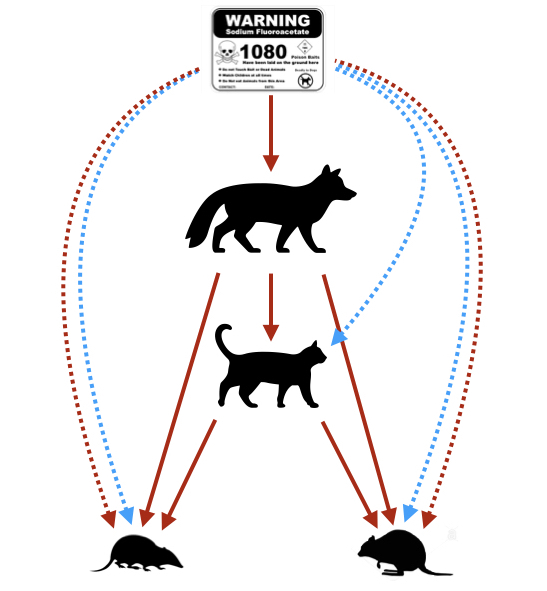
\includegraphics[width=0.7\linewidth]{figure/conceptual_diagram} 

}

\caption{Conceptual diagram of direct (solid line) and indirect (dashed line) positive (blue) and negative (red) interactions tested in this thesis. Fox control in Australia (in this case via 1080 poison-baiting) aims to suppress invasive red foxes, thereby benefiting two threatened prey species - the southern brown bandicoot and long-nosed potoroo. However, fox control may cause mesopredator release of feral cats (because foxes may exert top-down and competitive pressure on cats), which could lead to a net negative impact on their shared prey such as these two threatened native mammals.}\label{fig:intro-conceptual}
\end{figure}
\hypertarget{otways17}{%
\chapter{Unexpectedly high densities of feral cats in a rugged temperate forest}\label{otways17}}

\hypertarget{abstract}{%
\section*{Abstract}\label{abstract}}
\addcontentsline{toc}{section}{Abstract}

Effective invasive predator management requires accurate knowledge of population density. However, density can be difficult to estimate for wide-ranging, cryptic and trap-shy species, such as the feral cat \emph{Felis catus}. Consequently, few density estimates exist for this invasive predator of global significance, particularly from rugged, mesic or structurally complex habitats where detection is challenging. In this study, we estimated feral cat density in the wet forests and cool temperate rainforests of the Otway Ranges, south-eastern Australia, to (1) provide a density estimate for this rarely surveyed habitat type, and (2) verify predictions from a continental-scale model of feral cat density. We deployed 140 camera traps across two independent 49 km\textsuperscript{2} grids and identified individual feral cats based on unique pelage markings. Using spatially explicit mark-resight models, we estimated that there were 1.14 cats km\textsuperscript{-2} (95\% CI: 0.88 -- 1.47). This is more than three times the average cat density in natural environments across Australia, and at least five times higher than model-based predictions for the Otway Ranges. Such high densities of feral cats likely reflect the abundance of small native mammals and lack of apex predators in our study area. Our findings contradict the widespread assumption that feral cats occur at very low densities in mesic and rugged habitats. Underestimating the density of feral cats in these environments has significant implications for pest animal management and biodiversity conservation.

\newpage

\hypertarget{introduction}{%
\section{Introduction}\label{introduction}}

Accurate estimates of the distribution and abundance of invasive predators are essential to determine ecosystem impacts, inform effective management and target control efforts. However, this information is difficult to obtain as predators are often cryptic, trap-shy and occur at low densities (Royle \emph{et al.} 2008). A prominent example is the feral cat \emph{Felis catus}, which is implicated in the extinction or decline of 430 species globally (Doherty \emph{et al.} 2017). A better understanding of feral cat density has been highlighted as a priority for effective management of both this species and its threatened native prey (Woinarski \emph{et al.} 2014; Legge \emph{et al.} 2017; Moseby \emph{et al.} 2019).

Legge \emph{et al.} (2017) developed a continental-scale model of feral cat density for Australia which has had considerable implications for feral cat research and management. For instance, the model has been used to estimate the number of birds, reptiles and mammals killed annually across Australia by feral cats (Woinarski \emph{et al.} 2017, 2018; Murphy \emph{et al.} 2019). As the model estimated that there were considerably fewer feral cats in Australia than previously expected, it also casts doubt on the feasibility of Australian Federal Government's plan to cull two million feral cats between 2015 and 2020 (Doherty \emph{et al.} 2019). Given the importance of feral cat density estimates for policy, planning and management, it is vital to verify and refine the model's predictions.

The underlying data used by Legge \emph{et al.} (2017) had several limitations, including that feral cat density estimates were not available for any wetland, mangrove, dense heath or rainforest environments in Australia (Legge \emph{et al.} 2017). This likely reflects the difficulty of access and ineffectiveness of traditional feral cat monitoring methods (track counts and spotlight counts) in these structurally complex habitats (Denny \& Dickman 2010). Legge \emph{et al.} (2017) highlighted the need for more site-based density surveys, particularly in these under-studied environments. Further, nearly all of the density estimates collated by Legge \emph{et al.} (2017) were based on studies that did not identify individual cats or account for imperfect detection (i.e.~the possibility that some individuals were not detected). Such methods can be unreliable when inferring across sites, times, ecological contexts and different detection methods (Edwards \emph{et al.} 2000; Hayward \emph{et al.} 2015), particularly for species such as cats whose densities may fluctuate substantially over time in some regions (Legge \emph{et al.} 2017). Concurrent surveys of cats on Kangaroo Island and the adjacent Australian mainland suggests that the Legge \emph{et al.} (2017) model may substantially underestimate this variation in density (Taggart \emph{et al.} 2019).

Robust population density estimates for cryptic and wide-ranging species based on individual identification are now more feasible due to recent advances in technology and statistical models. Camera-traps that sense temperature-in-motion provide an efficient survey approach across diverse environments and are particularly beneficial for studies of trap-shy species with unique markings, such as feral cats (Bengsen \emph{et al.} 2011). Concurrently, spatial mark-resight (SMR) models, an extension of spatial capture-recapture models, enable population density estimates when a portion of the population can be individually identified (Royle \emph{et al.} 2013). These models consider both the distribution and movement of individuals across the landscape in relation to the placement of detectors, and account for imperfect detection (Royle \emph{et al.} 2013). The combination of camera-trap surveys to identify individuals and spatial capture-recapture methods to estimate density has shown promise for both feral and domestic cats (McGregor \emph{et al.} 2015b; Jiménez \emph{et al.} 2017; Robley \emph{et al.} 2017, 2018; Cove \emph{et al.} 2018).

The small number of studies that have estimated feral cat density in the mesic regions of south-eastern Australia indicate that these habitats support few feral cats relative to other regions (Legge \emph{et al.} 2017). However, survey effort for feral cats in these environments has been low compared to more arid regions. Our study therefore aimed to provide: (1) a density estimate for a rarely surveyed environment -- a matrix of wet forest and cool temperate rainforest, and (2) an independent verification of the prediction from the Legge \emph{et al.} (2017) continental-scale model of feral cat density for the Otway region. To achieve these aims, we undertook a camera-trap survey over 8,230 trap nights at 140 sites in the Otway Ranges, south-eastern Australia. We derived feral cat density estimates by applying SMR analysis to our camera survey data.

\newpage

\hypertarget{methods}{%
\section{Methods}\label{methods}}

\hypertarget{study-area}{%
\subsection{Study area}\label{study-area}}

Our study was conducted in the Great Otway National Park and Otway Forest Park, Victoria, Australia (38.42 °S, 142.24 °E). The locality is 90 -- 440 m above sea level. and has a cool-temperate climate: maximum daily temperatures average 19.3 °C in summer and 9.5 °C in winter; annual rainfall averages 1955 mm (Bureau of Meteorology 2021). The vegetation is a mosaic of old-growth shrubby wet forest, wet forest and cool temperate rainforest, with an overstorey of tall eucalyptus spp. (primarily \emph{Eucalyptus regnans}), \emph{Acacia melanoxylon} and \emph{Nothofagus cunninghamii}, and a midstorey dominated by tree ferns, \emph{Acacia verticillata}, \emph{Pomaderris aspera} and \emph{Olearia argophylla}. The understorey predominantly comprises a dense layer of ferns and graminoids, but is relatively open in steep gullies. The terrestrial predator guild is depauperate, with the introduced red fox \emph{Vulpes vulpes} being the only other significant competitor of feral cats. Our camera survey and other live-trapping surveys indicate an abundance of small native mammals within the study region, particularly native rats and antechinus (Banikos 2018).

\hypertarget{study-design}{%
\subsection{Study design}\label{study-design}}

We deployed camera traps in two grids, each approximately 49 km\textsuperscript{2} and separated by more than five kilometres (Fig. \ref{fig:otways17-map}). The northern grid comprised 67 survey sites, spaced an average of 526 m apart (86 -- 848 m). The southern grid comprised 73 survey sites, spaced an average of 547 m apart (352 -- 719 m). We deployed a Reconyx Hyperfire HC600 survey camera, with infrared flash and temperature-in-motion detector (Reconyx, Holmen, Wisconsin), at each site. Cameras functioned for 37 -- 68 days (mean 59) from 26 June to 2 September 2017, totalling 8230 trap nights. Each camera was placed on a tree approximately 30 cm above the ground and faced towards a lure 2 -- 2.5 m away. Vegetation in the camera's line of sight was cleared to prevent false triggers. The lure comprised an oil-absorbing cloth doused in tuna oil and placed inside a PVC pipe container with a mesh top. Ten to 30 small white feathers were also attached to the outside of the PVC pipe container. Each lure was fastened near the top of a one-metre wooden stake. Cameras took five immediately consecutive photographs when triggered, with no quiet period between trigger events.

\hypertarget{individual-cat-identification}{%
\subsection{Individual cat identification}\label{individual-cat-identification}}

Images of feral cats were first grouped as marked or unmarked (black) individuals. Although some black cats had small white neck/chest coat splotches, these were not always visible (cats often moved with their heads down), and so all black cats were considered unmarked to avoid double-counting. The marked portion were tabby cats with naturally unique coat markings. These were further classified into distinct groups: stripes \& spots, thick swirls, other markings (ginger, distinctive breeds etc.) and unknown (due to poor image quality). At least two independent observers identified individual cats from these groups based on matches in unique markings, predominantly on the front legs, torso and across both flanks. Observers collated folders of images of unique individuals for reference. Discrepancies between observers were reviewed together until consensus was reached. If no consensus was reached, the marked cat was considered unidentifiable.

\hypertarget{estimating-population-density}{%
\subsection{Estimating population density}\label{estimating-population-density}}

We used conventional SMR models for an unknown number of marked individuals (sighting-only) to estimate feral cat density. These models assume that uniquely marked cats are a random sample of the population, with the same movement ecology as unmarked cats. We fitted models using the `secr' R-package (v. 3.2.1; Efford 2021) in R (v. 3.5.2; R Core Team 2020), as per Efford \& Hunter (2018).

Capture histories were collapsed into 24-h occasions, beginning at midday each day (as this was the time of day with the lowest observed cat activity). We used a 3500 m buffer around the outermost coordinates of the trapping grids to ensure density was estimated over an area large enough to include the activity centres of all cats potentially exposed to our survey (Royle \emph{et al.} 2013); this distance is larger than the estimated average maximum width of home ranges of large, male cats close to this region (n = 3; B.A. Hradsky, unpublished data).

In SMR models, detectability is defined by two parameters: \emph{g}\textsubscript{0}, the probability of detecting an animal (per occasion) if a detector was to be placed in the part of its home range where most time is spent, and sigma, a spatial scale parameter relating to home range size. Animals are assumed to have approximately circular home ranges, with the probability of detection declining with distance from the home range centre. We tested three shapes of this decline in detection probability: half‐normal, hazard‐rate, and exponential, and used the detector function with the lowest Akaike's Information Criterion adjusted for small sample size (AICc; Burnham \& Anderson 2004) for subsequent model fitting.

As the lures may have decreased in potency over the sampling session, we tested for a linear trend in \emph{g}\textsubscript{0} over time. We also tested whether density differed between the two grids, with and without a linear time trend. We compared these models to the null model (where detection and density were kept constant across both grids) using AICc. Overdispersal in the unmarked sightings was adjusted for as per Efford \& Hunter (2018) and a spatial resolution of 0.6 of the sigma estimate was used for all models (Efford 2021).

\newpage

\(~\)

\(~\)

\(~\)
\begin{figure}

\hfill{}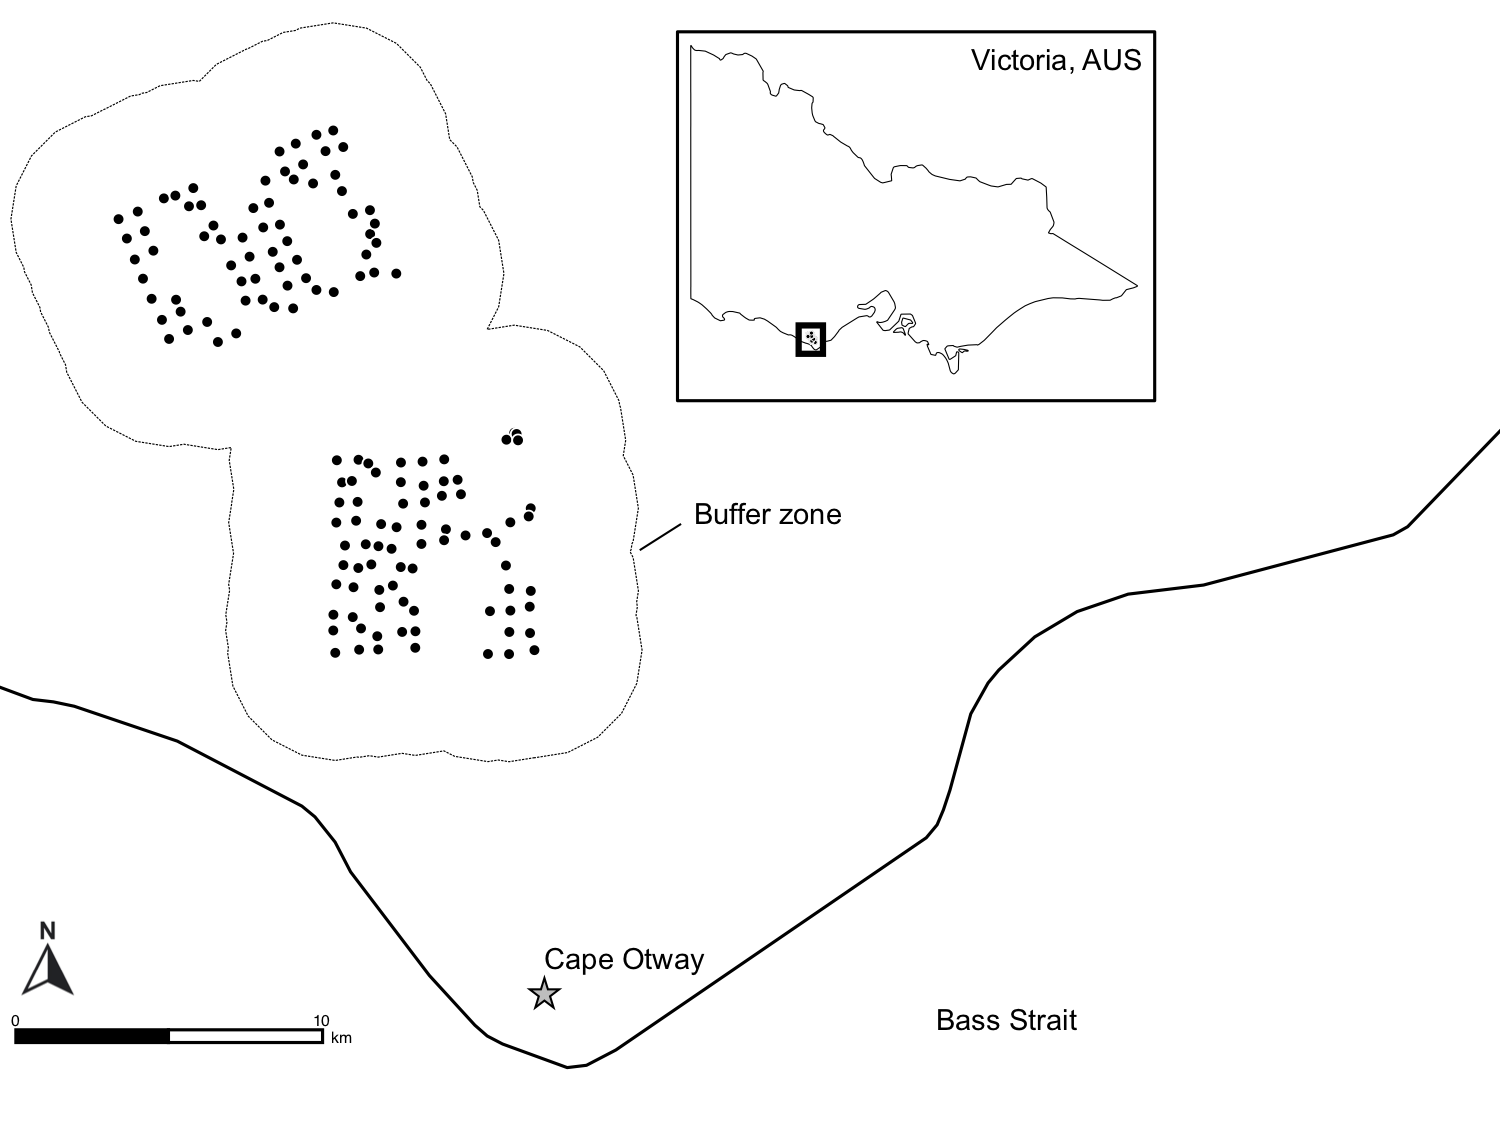
\includegraphics[width=1\linewidth]{figure/otways17_map} 

\caption{Study area, western Otway Ranges, Victoria, Australia, showing the location of the camera-trapping sites (black dots) within the 3500 m buffer zone (thin grey line).}\label{fig:otways17-map}
\end{figure}
\newpage

\hypertarget{results}{%
\section{Results}\label{results}}

We detected feral cats at 55\% of sites. Of these detections (1 detection = one or more visits of an individual/unidentifiable/unmarked cat to a camera-trap per 24-h occasion), 41\% were unmarked (black) cats. Of the marked cat detections, 89\% could be reliably identified to the individual-level -- 47 individuals were identified. The number of detections, number of identified individuals and mean distances moved were similar across the two camera-trapping grids (Table \ref{tab:otways17-stats}).

The top-ranked model estimated a density of 1.14 cats km\textsuperscript{-2} (95\% CI: 0.88 -- 1.47), with no difference in density between grids but a linear decrease in \emph{g}\textsubscript{0} over time (5.7\% decrease per week; Fig. \ref{fig:otways17-g0t}; Table \ref{tab:otways17-stats}). The second-ranked model (dAICc 1.74, Akaike weight 0.23) indicated that densities were slightly higher at the northern than southern grid, although confidence intervals overlapped substantially (Table \ref{tab:otways17-estimates}). The hazard-rate detector function best described the rate at which detection probability changed with the distance of the camera from the centre of a cat's home range (Table \ref{tab:otways17-detfn}). Estimates of feral cat density were robust to all model specifications, with the mean estimate varying by less than 0.2 cats km\textsuperscript{-2} between all models (Table \ref{tab:otways17-stats}).

\newpage

\(~\)

\(~\)

\(~\)
\begin{longtable}[]{@{}lccc@{}}
\caption{\label{tab:otways17-stats} Summary of raw camera survey data for feral cats in the Otway Ranges, Victoria, Australia, 2017.}\tabularnewline
\toprule
\begin{minipage}[b]{0.40\columnwidth}\raggedright
Summary statistic\strut
\end{minipage} & \begin{minipage}[b]{0.16\columnwidth}\centering
southern grid\strut
\end{minipage} & \begin{minipage}[b]{0.16\columnwidth}\centering
northern grid\strut
\end{minipage} & \begin{minipage}[b]{0.16\columnwidth}\centering
both grids\strut
\end{minipage}\tabularnewline
\midrule
\endfirsthead
\toprule
\begin{minipage}[b]{0.40\columnwidth}\raggedright
Summary statistic\strut
\end{minipage} & \begin{minipage}[b]{0.16\columnwidth}\centering
southern grid\strut
\end{minipage} & \begin{minipage}[b]{0.16\columnwidth}\centering
northern grid\strut
\end{minipage} & \begin{minipage}[b]{0.16\columnwidth}\centering
both grids\strut
\end{minipage}\tabularnewline
\midrule
\endhead
\begin{minipage}[t]{0.40\columnwidth}\raggedright
Number of camera sites\strut
\end{minipage} & \begin{minipage}[t]{0.16\columnwidth}\centering
73\strut
\end{minipage} & \begin{minipage}[t]{0.16\columnwidth}\centering
67\strut
\end{minipage} & \begin{minipage}[t]{0.16\columnwidth}\centering
140\strut
\end{minipage}\tabularnewline
\begin{minipage}[t]{0.40\columnwidth}\raggedright
Sites where cats detected (\%)\strut
\end{minipage} & \begin{minipage}[t]{0.16\columnwidth}\centering
51\strut
\end{minipage} & \begin{minipage}[t]{0.16\columnwidth}\centering
62\strut
\end{minipage} & \begin{minipage}[t]{0.16\columnwidth}\centering
55\strut
\end{minipage}\tabularnewline
\begin{minipage}[t]{0.40\columnwidth}\raggedright
Number of unmarked detection events\strut
\end{minipage} & \begin{minipage}[t]{0.16\columnwidth}\centering
47\strut
\end{minipage} & \begin{minipage}[t]{0.16\columnwidth}\centering
48\strut
\end{minipage} & \begin{minipage}[t]{0.16\columnwidth}\centering
95\strut
\end{minipage}\tabularnewline
\begin{minipage}[t]{0.40\columnwidth}\raggedright
Number of identifiable, marked detection events\strut
\end{minipage} & \begin{minipage}[t]{0.16\columnwidth}\centering
60\strut
\end{minipage} & \begin{minipage}[t]{0.16\columnwidth}\centering
59\strut
\end{minipage} & \begin{minipage}[t]{0.16\columnwidth}\centering
119\strut
\end{minipage}\tabularnewline
\begin{minipage}[t]{0.40\columnwidth}\raggedright
Number of unidentifiable, marked detection events\strut
\end{minipage} & \begin{minipage}[t]{0.16\columnwidth}\centering
10\strut
\end{minipage} & \begin{minipage}[t]{0.16\columnwidth}\centering
5\strut
\end{minipage} & \begin{minipage}[t]{0.16\columnwidth}\centering
15\strut
\end{minipage}\tabularnewline
\begin{minipage}[t]{0.40\columnwidth}\raggedright
Total number of identified individuals\strut
\end{minipage} & \begin{minipage}[t]{0.16\columnwidth}\centering
23\strut
\end{minipage} & \begin{minipage}[t]{0.16\columnwidth}\centering
24\strut
\end{minipage} & \begin{minipage}[t]{0.16\columnwidth}\centering
47\strut
\end{minipage}\tabularnewline
\begin{minipage}[t]{0.40\columnwidth}\raggedright
Number of cats resighted at different cameras\strut
\end{minipage} & \begin{minipage}[t]{0.16\columnwidth}\centering
8\strut
\end{minipage} & \begin{minipage}[t]{0.16\columnwidth}\centering
6\strut
\end{minipage} & \begin{minipage}[t]{0.16\columnwidth}\centering
14\strut
\end{minipage}\tabularnewline
\begin{minipage}[t]{0.40\columnwidth}\raggedright
Mean recapture distance (m)\strut
\end{minipage} & \begin{minipage}[t]{0.16\columnwidth}\centering
653\strut
\end{minipage} & \begin{minipage}[t]{0.16\columnwidth}\centering
774\strut
\end{minipage} & \begin{minipage}[t]{0.16\columnwidth}\centering
716\strut
\end{minipage}\tabularnewline
\begin{minipage}[t]{0.40\columnwidth}\raggedright
Maximum recapture distance (m)\strut
\end{minipage} & \begin{minipage}[t]{0.16\columnwidth}\centering
905\strut
\end{minipage} & \begin{minipage}[t]{0.16\columnwidth}\centering
1701\strut
\end{minipage} & \begin{minipage}[t]{0.16\columnwidth}\centering
1701\strut
\end{minipage}\tabularnewline
\bottomrule
\end{longtable}
\newpage

\(~\)

\(~\)

\(~\)
\begin{longtable}[t]{lllllllrrr}
\caption{\label{tab:otways17-estimates}Comparison of spatial mark-resight models and density estimates}\\
\toprule
\multicolumn{2}{c}{Model} & \multicolumn{4}{c}{Model comparison} & \multicolumn{4}{c}{Density estimate (cats km-2)} \\
\cmidrule(l{3pt}r{3pt}){1-2} \cmidrule(l{3pt}r{3pt}){3-6} \cmidrule(l{3pt}r{3pt}){7-10}
Density & g0 & K & AICc & dAICc & AICcwt & grid & estimate & lcl & ucl\\
\midrule
\endfirsthead
\caption[]{\label{tab:otways17-estimates}Comparison of spatial mark-resight models and density estimates \textit{(continued)}}\\
\toprule
\multicolumn{2}{c}{Model} & \multicolumn{4}{c}{Model comparison} & \multicolumn{4}{c}{Density estimate (cats km-2)} \\
\cmidrule(l{3pt}r{3pt}){1-2} \cmidrule(l{3pt}r{3pt}){3-6} \cmidrule(l{3pt}r{3pt}){7-10}
Density & g0 & K & AICc & dAICc & AICcwt & grid & estimate & lcl & ucl\\
\midrule
\endhead

\endfoot
\bottomrule
\endlastfoot
1 & T & 5 & 1568.84 & 0 & 0.71 & both & 1.14 & 0.88 & 1.47\\
grid & T & 6 & 1570.68 & 1.84 & 0.28 & north & 1.23 & 0.90 & 1.68\\
 &  &  &  &  &  & south & 1.05 & 0.78 & 1.42\\
1 & 1 & 4 & 1578.37 & 9.53 & 0.01 & both & 1.14 & 0.89 & 1.48\\
grid & 1 & 5 & 1579.66 & 10.82 & 0 & north & 1.25 & 0.91 & 1.72\\
\addlinespace
 &  &  &  &  &  & south & 1.04 & 0.77 & 1.40\\*
\end{longtable}
\emph{T = linear time trend}

\emph{K = number of parameters estimated}

\emph{AICc = Akaike's Information Criterion with small-sample adjustment}

\emph{dAICc = difference between AICc of this model and the model with smallest AICc}

\emph{AICcwt = AICc model weight}

\emph{lcl -- lower 95\% confidence limit}

\emph{ucl -- upper 95\% confidence limit}

\newpage

\hypertarget{discussion}{%
\section{Discussion}\label{discussion}}

Our work provides one of the first robust estimates of feral cat density for a temperate wet forest in Australia. Our estimate of 1.14 cats km\textsuperscript{-2} (95\% CI: 0.88 -- 1.47) is five times higher than that predicted by the Legge \emph{et al.} (2017) model for this location (0.17 - 0.23 cats km\textsuperscript{-2}), and more than three times higher than the predicted continental mean density for feral cats in `natural areas' (0.27 cats km\textsuperscript{-2}; 0.18 -- 0.45 cats km\textsuperscript{-2}; Legge \emph{et al.} 2017). The mesic coastal areas of Australia were previously thought to support the lowest densities of feral cats across the continent, particularly rugged and wet regions, such as rainforests (Dickman 1996; Johnson 2006; Legge \emph{et al.} 2017; McDonald \emph{et al.} 2017). Accordingly, feral cats were believed to have relatively less impact on native species in these environments (Burbidge \& Manly 2002; Doherty \emph{et al.} 2017; Woinarski \emph{et al.} 2017, 2018; Radford \emph{et al.} 2018; Murphy \emph{et al.} 2019). Our finding is therefore startling, and prompts a rethink about the threat that feral cats may pose to native fauna in mesic habitats.

The high density of feral cats in our study region likely reflects the high productivity of the landscape and abundant populations of some prey species. Our study region has the highest annual rainfall in Victoria (Bureau of Meteorology 2021), and live-trapping surveys in our study site show consistent, near saturation of small mammal traps, predominantly bush rats \emph{Rattus fuscipes} and \emph{Antechinus spp}. (Z. Banïkos, unpublished data). Several images from our study confirmed that feral cats prey upon these taxa. These small mammals may be relatively robust to introduced predators due to their high fecundity and generalist habitat requirements (e.g.~Banks 1999). However, by supporting high densities of feral cats, they may also facilitate high levels of predation on rarer and more vulnerable species (Smith \& Quin 1996), such as the now locally extinct smoky mouse \emph{Pseudomys fumeus} (Menkhorst \& Broome 2006). Significant declines and local extinctions of other small mammals have also been reported across the eastern Otways (Wayne \emph{et al.} 2017b). Understanding temporal trends in these predator-prey dynamics and the relationships between introduced predators and their native primary and alternative prey is a key priority for future research.

The lack of apex predators and competitors in the Otway Ranges may also facilitate high feral cat densities. Dingoes \emph{Canis familiaris}--higher order predators (Johnson \emph{et al.} 2007)--and tiger quolls \emph{Dasyurus maculatus}--key competitors (Glen \& Dickman 2005)--are functionally extinct in the Otway Ranges. We detected foxes at 25\% of sites (M. Rees, unpublished data) but the extent to which foxes exert top-down control on feral cats is unclear. Changes in feral cat abundance, behaviour and/or diet have been observed in response to fox control (Molsher \emph{et al.} 2017; Hunter \emph{et al.} 2018), and the relationship could be further clarified using robust density estimates under experimental manipulations of fox density.

The belief that feral cat densities in Australia are lower in mesic forests than open habitats stems partly from the lack of robust density estimates from forests, and partly from observations that cats have greater hunting success and are more detectable in open microhabitats (McGregor \emph{et al.} 2014, 2015b; Hohnen \emph{et al.} 2016; McDonald \emph{et al.} 2017) and select for savannah over rainforest (McGregor \emph{et al.} 2017). However, the variation in understorey structure (from extremely dense to relatively open) in our study region potentially creates ideal shelter and foraging habitat for feral cats, which often hunt along edges between dense and open vegetation (Doherty \emph{et al.} 2015a). Our findings challenge the belief that cat density is low in mesic forests, and instead concur with the global pattern that feral cats have smaller, overlapping home ranges in productive, low-seasonal environments, resulting in higher population densities (Bengsen \emph{et al.} 2016).

Our surveys clearly need replicating in other mesic environments before they can be generalised. Nonetheless, higher than expected densities of feral cats in mesic and complex environments would have serious implications for biodiversity conservation. Feral cats are thought to be a key driver of the recent declines of critical-weight-range mammals in northern Australia (Woinarski \emph{et al.} 2010; Fisher \emph{et al.} 2014; Davies \emph{et al.} 2018). Contemporary mammal declines are also occurring in temperate Australia, including the Otway Ranges (Bilney \emph{et al.} 2010; Wayne \emph{et al.} 2017a; Lindenmayer \emph{et al.} 2018). A better understanding of feral cat densities in these regions is essential for identifying key threatening processes and improving management outcomes.

In conclusion, our study shows that feral cats can occur at high densities in wet forests and cool temperate rainforests, contrary to previous expectations. Further research is needed to understand the impacts of this on native mammal populations, and the mechanisms that drive spatial variation in feral cat density, including the influence of habitat type, productivity, disturbance events and interactions with other predators. New spatial capture-recapture methods will likely play a powerful role in improving understanding of the ecology of this globally-significant predator. Our work provides a strong foundation for future investigations, as our methodology allows for robust evaluations of feral cat density, particularly under experimental manipulations and population comparisons.

\hypertarget{occ}{%
\chapter{Lethal fox control and fire influence the occurrence of invasive predators and threatened native prey}\label{occ}}

\hypertarget{abstract-1}{%
\section*{Abstract}\label{abstract-1}}
\addcontentsline{toc}{section}{Abstract}

Invasive predators and altered fire regimes are key, often overlapping biodiversity threats. Disentangling the impacts of multiple threats and management actions is challenging, particularly when species occur patchily across heterogeneous landscapes.

Here we assessed the effects of lethal control of an introduced apex predator, the red fox \emph{Vulpes vulpes}, on mammal communities in fire-prone and fragmented forests of south-eastern Australia. Our study synthesised data from multiple smaller-scale studies that used a combination of experimental and space-for-time approaches to monitor the effects of fox control and time since fire, giving a total of 3667 camera-traps deployments across 1232 sites (172,052 trap nights). We used occupancy-detection models to investigate species detectability, and generalised additive models to explore potentially nonlinear effects of multiple drivers and management actions on the distribution of two invasive mammalian predators and two threatened native prey species.

In one region with frequent, long-term (8 - 14 years) targeted poison-baiting of foxes, foxes were heavily suppressed in terms of both detectability and occupancy. There was some evidence feral cat \emph{Felis catus} occupancy was slightly higher in landscapes with fox control, potentially signalling mesopredator release. Fox control increased occupancy rates of long-nosed potoroos \emph{Potorous tridactylus}, but had little effect on occupancy rates of the southern brown bandicoot \emph{Isoodon obesulus}. In another region where fox control recently commenced (0 - 2 years), foxes were suppressed to a lesser extent, and no impacts were detected on subordinate predator or prey species. Fire history impacted the occurrence of each study species, however, invasive predators responded differently to time since fire (0 - 80 years) across each vegetation type.

Predator control and prescribed fire are important tools that can be used by land managers to manipulate mammalian communities. However, the effectiveness of lethal predator control depends on the intensity and duration of management, and optimal fire regimes differ between species and vegetation types.

\newpage

\hypertarget{introduction-1}{%
\section{Introduction}\label{introduction-1}}

Accurate and precise estimates of the effects of management are essential to inform conservation decision-making, ensure cost-effective allocation of resources and identify potential unintended consequences of interventions (Christie \emph{et al.} 2020). However, reliable inference about the effects of landscape-scale management, including identifying the cause of nil or perverse outcomes, is often difficult to achieve because target populations fluctuate naturally and are often subject to multiple co-occurring threats and management actions (Pressey \emph{et al.} 2007; Sugihara \emph{et al.} 2012). Separating management effects from other drivers is particularly difficult for species that occur patchily across broad distributions (Tulloch \emph{et al.} 2016).

Invasive predator management is a classic example of these challenges. Predators can have devastating impacts on native biodiversity when introduced beyond their native range, and so are often actively controlled using lethal methods (Sih \emph{et al.} 2010; Bellard \emph{et al.} 2016; Doherty \emph{et al.} 2016). Quantifying the degree of invasive predator suppression, the responses of their native prey and any unintended outcomes across gradients of predator control is key to designing effective, cost-efficient management programs (Baxter \emph{et al.} 2008; Walsh \emph{et al.} 2012; Cattarino \emph{et al.} 2016). However, the ability of associated monitoring programs to detect these signals is often limited by confounding from co-occurring threats, management actions or natural drivers. This is concerning because few or negative effects on native biodiversity are often observed following invasive predator control, particularly when multiple introduced species are present (Ballari \emph{et al.} 2016).

There are several explanations for why native prey species may not benefit from introduced predator control. Firstly, invasive predators may not be suppressed below tolerable thresholds--predators can be remarkably resilient to low-effort culling (Sinclair \emph{et al.} 1998; Sabo 2005; Lazenby \emph{et al.} 2015; Moseby \emph{et al.} 2019). Secondly, predation by introduced species may not be the primary limit on native prey populations (Banks 1999). Thirdly, invasive predator suppression may lead to a `release' of a subordinate predator (Courchamp \emph{et al.} 1999; Crooks \& Soulé 1999) or competitor species (Ruscoe \emph{et al.} 2011), which could potentially worsen outcomes (e.g., Rayner \emph{et al.} 2007). Hence, quantifying the degree of apex predator suppression and testing the mesopredator release hypothesis (Prugh \emph{et al.} 2009), are important steps toward understanding prey responses to lethal predator control.

Quantifying the impacts of planned fire on fauna is similarly complex. Fire can drive the persistence and abundance of fauna populations, primarily through its effects of vegetation structure (Monamy \& Fox 2000). These effects persist for decades or centuries, are nonlinear, and vary across environmental conditions (Haslem \emph{et al.} 2011). Fauna species can have variable responses to fire across heterogeneous landscapes because post-fire regeneration of habitat structure and quality varies across ecological communities and ecological conditions (Nimmo \emph{et al.} 2014; Swan \emph{et al.} 2015). Predicting the long-term ramifications of fire on predators and prey is a key challenge for managers who are tasked with stemming the decline of native fauna populations while simultaneously managing fuel loads to protect against the increasing threat of large wildfires (Clarke 2008; Hradsky 2020).

Disentangling the complex and potentially interacting effects of invasive predator and fire management on threatened native fauna is crucial for effective fauna conservation in Australia, which has experienced some of the worst biodiversity declines in recent world history (Doherty \emph{et al.} 2015c; Waldron \emph{et al.} 2017; Woinarski \emph{et al.} 2019). Predation by introduced species and altered fire regimes are clearly primary drivers of the declines and contemporary distributions of native mammals (Woinarski \emph{et al.} 2015), but other threatening processes such as habitat fragmentation, and natural drivers such vegetation type and rainfall dynamics also play an important role (May \& Norton 1996; Hale \emph{et al.} 2016). Lethal red fox \emph{Vulpes vulpes} (hereafter `fox') control and prescribed burning (primarily for asset protection) are among the most common management actions in protected areas, however, we have a poor understanding of effects on native fauna (Clarke 2008; McLeod \emph{et al.} 2008; Braysher 2017; Lindenmayer \emph{et al.} 2018; Hradsky 2020). This is partly because there is strong spatial overlap of these threats and management actions (Evans \emph{et al.} 2011) and potential unintended consequences often go unmeasured.

In this study we assessed the effect of two landscape-scale lethal management programs on foxes in fire-prone regions of south-eastern Australia. We quantified the effects of management on foxes (the managed species), feral cats \emph{Felis catus} (hereafter `cat'; unmanaged competitor), and two threatened species that are the primary focus of the conservation programs: the southern brown bandicoot \emph{Isoodon obesulus} (hereafter `SBB') and long-nosed potoroo \emph{Potorous tridactylus} (hereafter `LNP'). Our study dataset combined experimental and space-for-time approaches to support understanding of the effects of management and other drivers on invasive predator and threatened native prey populations in two regions of southeastern Australia; the Glenelg region and Otway Ranges. Monitoring of the outcomes of management was based on one-off and repeat deployments of 3667 camera-traps across 1232 sites over a period of seven years in protected conservation areas. In the Glenelg region, foxes had been continuously controlled for 8 - 14 years in approximately half of the region and another region where fox control recently commenced (monitored 1 year prior and 2 years following fox control which occurs in approximately 75\% of the surveyed region). Occupancy-detection models (MacKenzie \emph{et al.} 2002) were used to investigate the detectability of each species. Occurrence probabilities were also analysed for each species using Generalised Additive Models (hereafter ``GAMs''; Wood 2017), which did not account for imperfect detection, but allowed nonlinear responses and more complex interactions between predictor variables. We used GAMs to explore the potentially nonlinear responses of species to fox control effort (1080 poison-bait density), time since fire (0 - 80 years) across vegetation types and other environmental drivers (elevation, terrain ruggedness, recent rainfall, topographic wetness, fragmentation).

\newpage

\hypertarget{methods-1}{%
\section{Methods}\label{methods-1}}

\hypertarget{study-regions}{%
\subsection{Study regions}\label{study-regions}}

We compiled data from multiple camera-trap studies across two regions in south-west Victoria, Australia: the Glenelg region and Otway Ranges (Fig. \ref{fig:occ-map}). Introduced foxes and cats are the only medium-large functional mammalian terrestrial carnivores here: native dingoes \emph{Canis familiaris} are long-absent throughout, while tiger quolls \emph{Dasyurus maculatus} are long-absent in the Glenelg region and likely functionally extinct in the Otway Ranges (last confirmed sighting in 2014).

\hypertarget{glenelg-region}{%
\subsubsection{Glenelg region}\label{glenelg-region}}

In the Glenelg region (38°05'54``S 141°44'41''E), large patches of natural vegetation are fragmented mostly by pastoral farming and residential properties (Fig. \ref{fig:occ-map}). Here, the primary vegetation communities are heathy woodland, lowland forest, herb-rich woodland and wet heathland (Department of Environment, Land, Water \& Planning 2020a). The Glenelg region has an annual mean minimum temperature of 8.1 °C in winter, and 20.0 °C in Summer (Bureau of Meteorology 2021). Mean annual rainfall averages 835 mm (Bureau of Meteorology 2021). Terrain is gently undulating in the Glenelg region; our study sites range from 12 - 180 m above sea level.

\hypertarget{otway-ranges}{%
\subsubsection{Otway Ranges}\label{otway-ranges}}

The Otway Ranges (38°57'82``S 141°68'41''E) is a largely continuous patch of natural vegetation with a strong east-west rainfall gradient (Fig. \ref{fig:occ-map}). A matrix of cool temperate rainforest and wet forest at high-altitudes (up in the south-west descend into a large heathland directly north, and into dry forests and then heathlands to the north-east. Annual rainfall averages 1955 mm in the southwest, dropping to 627 mm in the eastern Otways (Bureau of Meteorology 2021). Mean minimum temperature in the Otway Ranges is 8° in winter and 13° in summer (Bureau of Meteorology 2021). Our study sites ranged from 23 - 617 m above sea level.

\hypertarget{fox-control-and-monitoring}{%
\subsection{Fox control and monitoring}\label{fox-control-and-monitoring}}

In broad sections of each region, government land managers conduct ongoing targeted lethal fox control for biodiversity conservation. Poison-baits containing 3 mg of sodium mono-fluroacetate (`1080') are buried at a depth of 12 - 15 cm at 1-km intervals along accessible forest tracks and roads. Different road densities result in spatially variable densities of poison-bait. Managers also frequently implement prescribed fire across both regions, primarily to reduce fuel loads.

\hypertarget{glenelg-region-1}{%
\subsubsection{Glenelg region}\label{glenelg-region-1}}

In the Glenelg region, foxes in three distinct forest blocks have been subject to poison-baiting since October 2005, with fortnightly bait replacements. These forest blocks, along with three similar, unbaited forest blocks to the north are simultaneously surveyed annually under the `Glenelg Ark' fox control program (40 camera-sites per block; Robley \emph{et al.} 2020). Hair-tubes were used to monitor small prey species from 2005 - 2013 (presented in Robley \emph{et al.} 2014), replaced by camera-traps from 2013 onwards (here we present camera-trap data from 2013 - 2019; Robley \emph{et al.} 2020). We also included a further 425 camera-trap deployments at unique locations from early 2018 (M.W.R., PhD surveys). This totals 2039 camera-trap deployments in the Glenelg region, collected in a control-impact experimental design (foxes had been continuously controlled for at 8 - 14 years in the treatment landscapes by the time of these surveys).

\hypertarget{otway-ranges-1}{%
\subsubsection{Otway Ranges}\label{otway-ranges-1}}

Fox-baiting commenced in small sections of the Otway Ranges in 2008 and large-scale systematic baiting began in 2016 - 2017 under the `Otway Ark' program (Robley \emph{et al.} 2019). For the first six weeks, poison-baits were replaced weekly, then changing to ongoing monthly bait-replacement. There was a pause in baiting for approximately six months during the second half of 2018. Fox control recommenced in late 2018 with four weeks of fortnightly bait-replacement, before returning to monthly bait-replacement. A large section of the Otway Ranges to the north-west remains unbaited, but is monitored as an experimental non-treatment site (Robley \emph{et al.} 2019). Otway Ark managers survey 372 camera-trap sites annually (sequentially across the region); we present one `before' baiting survey and two `after' baiting surveys of each site from 2016 - 2018, totalling 1113 camera-trap deployments (Robley \emph{et al.} 2019). We also include data from an additional before-after control-impact surveys (one `before' baiting survey and two `after' bating surveys) in the western section of the Otway Ranges, conducted annually 2017 - 2019 (M.W.R PhD surveys). This added a further 195 sites and 524 camera-trap deployments.

\hypertarget{camera-trap-set-ups}{%
\subsubsection{Camera-trap set-ups}\label{camera-trap-set-ups}}

All camera-trap deployments consisted of a Reconyx (Holmen, Wisconsin) brand camera-trap (white or infrared flash), attached to a tree or a metal picket, facing a lure. The Glenelg Ark and Otway Ark fox monitoring programs positioned camera-traps at least 40 cm above ground on a tree or a metal picket and angled more strongly downwards toward a lure approximately 1 - 1.5 m away (Robley \emph{et al.} 2019, 2020). The lures consisted of peanut butter, golden syrup and rolled oats mixed into a small ball, placed within a tea strainer or PVC pipe container and secured either to the ground, or 20 - 60 cm above ground on a wooden stake. The M.W.R. PhD surveys across both regions positioned camera-traps lower on a tree (around 15 - 30 cm above the ground) angled only slightly downwards towards a tuna oil lure approximately 2 - 2.5 m away (detailed in Rees \emph{et al.} 2019). Camera-traps were active for an average of 47 days (maximum 93 days), totalling 172,052 trap-nights.

\hypertarget{study-species-1}{%
\subsubsection{Study species}\label{study-species-1}}

Foxes and feral cats are both introduced to Australia and share a similar functional niche (Glen \& Dickman 2005), competing for many of the same prey species (Stobo-Wilson \emph{et al.} 2021a, b; Woinarski \emph{et al.} 2021). LNPs and SBBs are both solitary, medium-sized, ground-dwelling marsupials. They nest in dense understorey vegetation during the day and turn over large quantities of soil to feed on invertebrates, plant material and fungi at night (Van Dyck \& Strahan 2008).

\hypertarget{occupancy-detection-models}{%
\subsection{Occupancy-detection models}\label{occupancy-detection-models}}

We first modelled species occupancy probabilities using occupancy-detection models (MacKenzie \emph{et al.} 2002) implemented in a Bayesian framework using `stan' (Carpenter \emph{et al.} 2017) via the `ubms' R-package (Kellner 2021). For each species, we fit a `stacked' single-season model: repeat surveys were considered as additional sites and pseudoreplication accounted for by using a random-intercept for each unique site. We defined survey occasions as 24-hour periods commencing at midday. We modelled the effect of fox control (categorical: baited or unbaited) on species occupancy and detectability, and included an interaction term with region to account for potentially different responses in the Glenelg and Otway regions. This approach allowed combination of the regional datasets, increasing statistical power to detect smaller effects and precision of parameter estimates. We fit models with four MCMC chains each with 10,000 iterations (including a 5000-iteration warm-up phase). To determine whether detection probabilities for these surveys were high enough to justify analysis with generalised additive models (which do not account for imperfect detections), we calculated cumulative detection probabilities for camera-trap survey lengths (Garrard \emph{et al.} 2008) from one to 93 days (maximum survey duration).

\hypertarget{generalised-additive-models}{%
\subsection{Generalised additive models}\label{generalised-additive-models}}

We modelled species occurrence probabilities using binomial GAMs implemented in the `mgcv' R-package (Wood 2017). The use of GAMS has the advantage of allowing modelling of non-parametric and nonlinear relationships between occurrence and explanatory variables, which is particularly important for estimating time since fire responses (Haslem \emph{et al.} 2011). Relative to occurrence-detection models, GAMs allow more complex model structures to be fit in a computationally efficient framework, but assume perfect detection. For the most part, we considered this a reasonable assumption; the occurrence-detection models revealed high (\textgreater{} 75\%) cumulative detection probabilities based on our average camera-trap survey effort for each species across baited and unbaited landscapes for each region, except for cats in the Glenelg region (see results for details).

Our GAMs used a binary occupied-unoccupied response variable for each entire camera-trap deployment. To account for differences in survey duration, we specified a model offset for the log-transformed survey duration (number of days), as well as a random intercept for each unique camera-site to account for repeat sampling. We used the double penalty model selection approach, which penalises model complexity both in terms of the model structure (variables included) and the shapes (wiggliness) of the relationships between the dependent and independent variables included in the model (Marra \& Wood 2011). We used the same model structure and explanatory variables, for each species, as detailed in the sections below.

\hypertarget{poison-bait-density}{%
\subsubsection{1080 poison-bait density}\label{poison-bait-density}}

Poison-baits are deployed by land managers to suppress foxes with the aim of benefiting native prey. However, cats may also benefit from fox control as they are subordinate competitors to foxes (Marlow \emph{et al.} 2015b; Hunter \emph{et al.} 2018). The degree of fox suppression is a function of the spatial arrangement of poison baits (i.e., poison-bait density) relative to fox home-range size, as well as the frequency of bait replacement (Fleming 1996; Benshemesh \emph{et al.} 2020). In the Otway and Glenelg regions, adult foxes travel an average maximum distance of 2.3 km from their home-range centre (Hradsky \emph{et al.} 2017c). Therefore, to examine the effects of lethal control effort we summed the number of poison-bait stations within a 2.3 km radius around each camera-trap deployment. Densities ranged from 0 - 19 baits per 16.1 km\textsuperscript{2} circle (2.3 km radius): mean: 10 and eight baits per fox home-range in fox-baited landscapes in the Glenelg region and Otway Ranges, respectively. For an easier comparison to other studies, we converted these values to baits per square kilometre. We modelled a function of 1080 poison-bait density with separate responses per region. In wet weather conditions, some poison-bait stations become inaccessible and baits do not get replaced, but we did not account for this because we lacked specific information. There was also an approximate six month pause in bait replacements in the Otway Ranges that we did not account for because it would have ignored prior fox suppression.

\hypertarget{fire-and-vegetation-type}{%
\subsubsection{Fire and vegetation type}\label{fire-and-vegetation-type}}

We modelled an interaction between time since fire (in years; hereafter `TSF') and vegetation type as we expected species occurrence to (i) differ across vegetation types, (ii) respond to TSF, and (iii) have variable responses to TSF in each vegetation type (as post-fire regeneration occurs at different speeds; Swan \emph{et al.} 2015). We also expected species to respond to fire frequency, as this can have a strong effect on vegetation structure (Collins \emph{et al.} 2012).

We derived fire frequency (the number of previous fires) and time since last fire (in years) for each camera trap deployment using coarse fire scar mapping provided by government managers, dating back to 1939 when large wildfires burnt both regions extensively. The most frequently burnt sites (n = 2) had experienced eight fires since 1939 (mean 1.5 fires), 397 sites had not burnt since 1939. We identified the Ecological Vegetation Class group (hereafter ``vegetation type''; standard units for vegetation classification in Victoria; Department of Environment, Land, Water \& Planning 2020a) for each unique camera-trap site, totalling eight vegetation types. We only surveyed 20 unique sites in rainforests, which are interspersed (primarily in low lying gullies) throughout wet and damp forests in the south-eastern Otway Ranges. Given the similarity, fine-scale interspersion of these EVC groups, and that both rarely or never experience fire, we merged them together (hereafter referred to as `wet forests').

We specified the TSF and vegetation type interaction with a hierarchical model structure, which estimated an average TSF response along with separate responses to TSF in each vegetation type (model ``GS'' detailed in Pedersen \emph{et al.} 2019). This shares information on TSF responses and wiggliness across EVC groups, penalising functions which deviate strongly from the average response that are not substantially supported by the observation data. We initially fit a separate smooth for fire frequency, however, this had high concurvity with TSF (causing a lack of identifiability) and so we removed the fire frequency variable from all models.

\hypertarget{elevation-topographic-ruggedness-and-wetness}{%
\subsubsection{Elevation, topographic ruggedness and wetness}\label{elevation-topographic-ruggedness-and-wetness}}

We modelled the effect of elevation, as well as indexes of topographic ruggedness and wetness (both derived from a digital elevation model) on species occurrences. Elevation is a strong driver of rainfall, moisture and temperature gradients, likely indirectly impacting the distribution of study species through resource availability. High topographic complexity (i.e., `ruggedness') can limit predator movement and predation rates, thereby benefiting prey (McKenzie \emph{et al.} 2007; Hohnen \emph{et al.} 2016; McDonald \emph{et al.} 2017; Stobo-Wilson \emph{et al.} 2020b). Soil moisture (estimated by the topographic wetness index) impacts vegetation, as well as the availability of subterranean invertebrates and fungi - key food sources for the LNP and SBB (Lobert 1990; Nuske \emph{et al.} 2017).

We extracted the elevation above sea level (metres) of each site using a 10-m resolution digital elevation model (Department of Environment, Land, Water \& Planning 2020b). We also used this elevation layer to calculate the median terrain ruggedness index (calculates the difference in elevation between a central cell and eight adjacent cells; Riley \emph{et al.} 1999), taking the median value in a 30-m radius around each camera-trap site. The topographic wetness index estimates where water will accumulate by accounting for topographic influences on hydrological processes (Beven \& Kirkby 1979). We also took the median topographic wetness index in a 30-m radius around each camera-trap site, derived from a 30-m resolution layer (Gallant \& Austin 2012). We modelled the effect of elevation, topographic ruggedness and wetness on species occurrences across both regions.

\hypertarget{proximity-to-forest-edge}{%
\subsubsection{Proximity to forest edge}\label{proximity-to-forest-edge}}

Invasive predators are well-documented to prefer edges between forest and cleared land as they facilitate efficient movement and hunting (May \& Norton 1996; Hradsky \emph{et al.} 2017c; Nichols \emph{et al.} 2019). We therefore modelled the effect of the minimum distance from each camera-trap site to the nearest area of non-native vegetation. We calculated this by inverting the extent of native vegetation (Department of Environment, Land, Water \& Planning 2019) and removing cleared areas smaller than 30 ha (Geary \emph{et al.} 2020b).

\hypertarget{recent-rainfall}{%
\subsubsection{Recent rainfall}\label{recent-rainfall}}

Changes in short-term rainfall dynamics likely impact both invasive predator and native prey species (Arthur \emph{et al.} 2012; Wilson \emph{et al.} 2012; Paull \emph{et al.} 2013; Greenville \emph{et al.} 2014). We therefore calculated the percentage difference in rainfall from the long-term median that had occurred prior to the start of each camera-trap survey in six, 12, 18 and 24 month periods. We used rainfall data from the nearest weather station (n = 11; Bureau of Meteorology 2021) for each camera-trap. We modelled rainfall effects separately for each region. To identify the most appropriate rainfall window (six -- 24 months) for each species, we fit a separate model (including all explanatory variables previously mentioned) using each rainfall window and selected the top-ranked model using Akaike Information Criterion (hereafter `AIC') scores (Burnham \& Anderson 2004).

All analyses were conducted in R version 3.6.3 (R Core Team 2020).

\newpage

\(~\)

\(~\)

\(~\)
\begin{figure}

{\centering 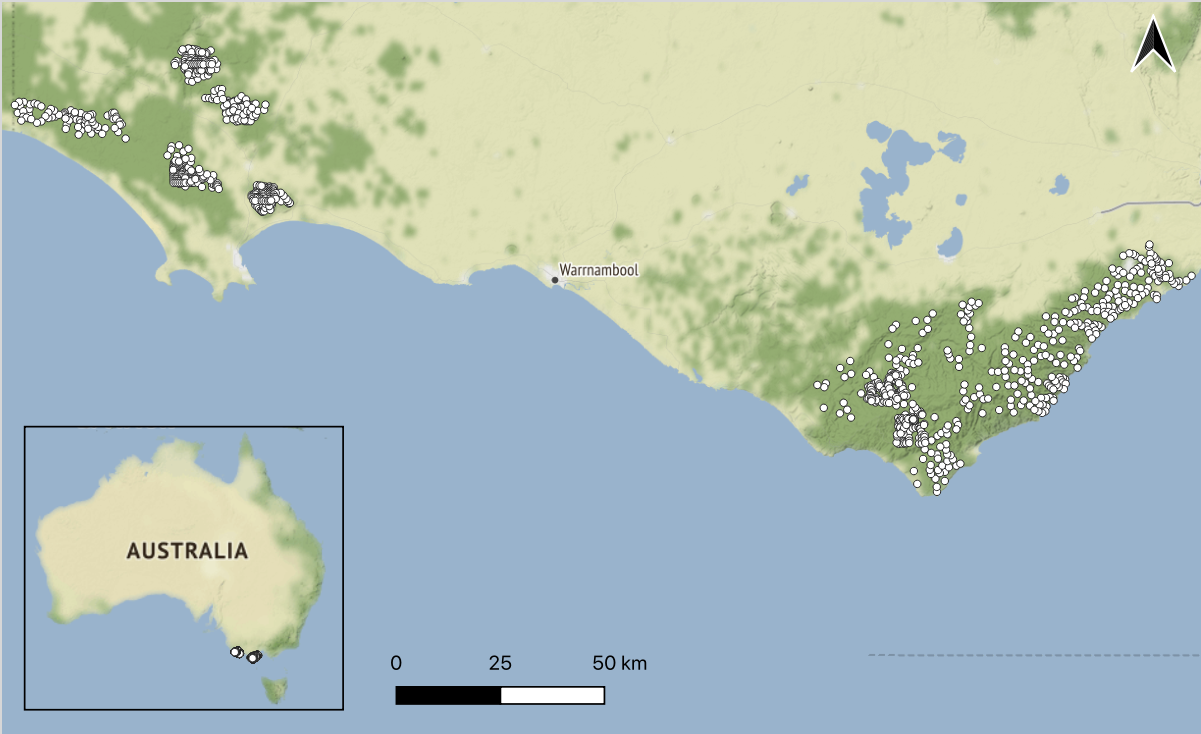
\includegraphics[width=1\linewidth]{figure/map_cams} 

}

\caption{Locations of study sites in south-west Victoria, Australia. The grids of camera-traps are denoted by white dots. The Glenelg region is to the west and Otway region to the east. Native vegetation is indicated by dark green, with hill shading. Map tiles by Stamen Design, under CC BY 3.0, map data by OpenStreetMap, under CC BY SA.}\label{fig:occ-map}
\end{figure}
\newpage

\hypertarget{results-1}{%
\section{Results}\label{results-1}}

\hypertarget{red-fox-1}{%
\subsection{Red fox}\label{red-fox-1}}

Foxes were detected on 1453 of the 3667 camera-traps surveys (39.6\%; Table \ref{tab:occ-naive}).

\hypertarget{occupancy-detection-models-1}{%
\subsubsection{Occupancy-detection models}\label{occupancy-detection-models-1}}

Fox detectability in unbaited landscapes was high, particularly in the Glenelg region (Fig. \ref{fig:occ-det}a) where 95\% detection probability was reached after a 30 day survey duration (relative to 64 days in the Otway Ranges; Fig. \ref{fig:occ-cumdet}). Fox control reduced fox detectability across both regions. Nonetheless, foxes in baited landscapes still had a high detection probability for the average survey duration (47 days): 76\% in the Glenelg region and 81\% in the Otway Ranges (Fig. \ref{fig:occ-cumdet}).

The occupancy-detection model estimated fox occupancy to be lower at sites in baited landscapes than unbaited landscapes; this effect was more than twice as strong in the Glenelg region than the Otway Ranges (Fig. \ref{fig:occ-det}b). For example, in heathy woodlands of the Glenelg region, fox occupancy probability was approximately three times lower in baited landscapes (0.19; 95\% CI 0.13 - 0.26) relative to unbaited landscapes (0.56; 95\% CI: 0.47 - 0.66). Whereas in the heathy woodlands of the Otway Ranges, fox occupancy was already low without fox control (0.33; 95\% CI: 0.25 - 0.43) and was approximately 1.4 times lower following fox control (0.24; 95\% CI 0.17 - 0.33). Foxes were ubiquitous across the study regions, but the probability of occupancy was nearly twice as high in dry forests, herb-rich woodlands and lowland forests than heathlands, heathy woodlands and wet forests (Fig. \ref{fig:occ-det}c).

\hypertarget{generalised-additive-models-1}{%
\subsubsection{Generalised additive models}\label{generalised-additive-models-1}}

The GAM showed that fox-bait density in the Glenelg region was the strongest driver of fox occurrence. Fox occurrence in the Glenelg region declined from a probability of 0.68 (95\% CI: 0.58 - 0.76) where fox-bait density was zero, to 0.04 (95\% CI: 0.02 - 0.11) where fox-bait density was highest (1.14 baits km\textsuperscript{-2}; Fig. \ref{fig:gams-occ-fox}a). The effect of fox-bait density on foxes in the Glenelg region was nonlinear: there was little difference in fox occurrence across the range of 0.4 to 0.8 baits km\textsuperscript{-2} in Glenelg, but a greater suppression was achieved at higher bait densities (Fig. \ref{fig:gams-occ-fox}a). Fox occurrence also declined with fox-bait density in the Otway Ranges, but this effect was linear, weaker and had higher uncertainty (Fig. \ref{fig:gams-occ-fox}a). Fox occurrence in the Otway Ranges declined from a probability of 0.4 (95\% CI: 0.32 - 0.48) where fox-bait density was zero, to 0.14 (95\% CI: 0.05 - 0.35) where fox-bait density was highest (1.1 baits km\textsuperscript{-2}; Fig. \ref{fig:gams-occ-fox}a).

Foxes declined linearly with increasing terrain ruggedness and distance to non-native vegetation for up to 1.5 - 2 km (Fig. \ref{fig:gams-occ-fox}d;f). Elevation had a nonlinear and uncertain effect on fox occurrence, which was estimated to peak around 450 m above sea level (Fig. \ref{fig:gams-occ-fox}c). The effect of topographic wetness on fox occurrence was removed from the model (Fig. \ref{fig:gams-occ-fox}e). There was no average TSF response on fox occurrence, however, fox occurrence declined linearly with TSF in dry forests and increased linearly with TSF in heathland, although there was considerable uncertainty in these estimates (Fig. \ref{fig:gams-occ-fox}g:h). The fox GAM that considered rainfall deviations in the previous 6 months was ranked highest relative to models with 18- (by only 1.4 AIC units), 12-, and 24-month periods (by at least 6.4 AIC units; Table. \ref{tab:occ-rain-aic}, however, this effect was weak with relatively high uncertainty (Fig. \ref{fig:gams-occ-fox}c). The top-ranked fox GAM had an adjusted R-square value of 0.27 and explained 26\% of the null deviance.

\hypertarget{feral-cat-1}{%
\subsection{Feral cat}\label{feral-cat-1}}

Cats were detected on 1010 camera-trap deployments (27.6\%; Table \ref{tab:occ-naive}).

\hypertarget{occupancy-detection-models-2}{%
\subsubsection{Occupancy-detection models}\label{occupancy-detection-models-2}}

Cats were relatively poorly detected in the Glenelg region, where they had a 59\% detection probability for the average survey duration, compared to 83\% in the Otway Ranges; Fig. \ref{fig:occ-cumdet}). There was no detectability difference between fox control treatment landscapes in the Glenelg region, however, cat detectability was slightly higher with fox control in the Otway Ranges (Fig. \ref{fig:occ-det}a).

The occupancy-detection models estimated that cat occupancy in the Glenelg region was higher in landscapes with fox control (0.25 in heathy woodlands; 95\% CI: 0.16 - 0.35 in heathy woodlands) relative to those without fox control (0.12 in heathy woodlands; 95\% CI: 0.07 - 0.19); but there was no association with baiting in the Otway Ranges (Fig. \ref{fig:occ-det}b). Cat occupancy was most strongly driven by vegetation type: highest in the wet forest, followed by heathland, swampy scrub, herb-rich woodland and dry forest, but very low in lowland forest and heathy woodland (Fig. \ref{fig:occ-det}c).

\hypertarget{generalised-additive-models-2}{%
\subsubsection{Generalised additive models}\label{generalised-additive-models-2}}

The cat GAM showed no effect of fox-bait density, elevation or topographic wetness on cat occurrence (Fig. \ref{fig:gams-occ-cat}a;c;e). Cats responded to TSF differently across each vegetation type, with the average TSF response removed from the model (Fig. \ref{fig:gams-occ-cat}g:h). Cat occurrence probability increased with terrain ruggedness, and declined with distance from the nearest area of non-native vegetation, although uncertainty was high (Fig. \ref{fig:gams-occ-cat}d;f). All cat GAMs were indistinguishable based on AIC scores. The model which considered rainfall deviations in the previous six months explained slightly more variation in cat occupancy (0.7 AIC units lower) than models considering rainfall over longer time periods (Table. \ref{tab:occ-rain-aic}), estimating that cat occurrence slightly increased as rainfall increased (relative to the long-term average; Fig. \ref{fig:gams-occ-cat}c). All other GAMs had the rainfall variable removed. The top-ranked cat GAM had an adjusted R-square value of 0.24 and explained 24\% of the null deviance.

\hypertarget{southern-brown-bandicoot-1}{%
\subsection{Southern brown bandicoot}\label{southern-brown-bandicoot-1}}

We detected SBBs on 394 of the 3667 camera-traps (10.7\%; Table \ref{tab:occ-naive}).

\hypertarget{occupancy-detection-models-3}{%
\subsubsection{Occupancy-detection models}\label{occupancy-detection-models-3}}

SBBs were highly detectable, with a greater than 95\% detection probability reached after 31 and 43 days in the Glenelg and Otway Ranges, respectively (Fig. \ref{fig:occ-cumdet}). Baiting was associated with a decrease in SBB detectability in Glenelg but an increase in detectability in the Otways (Fig. \ref{fig:occ-det}a).

There was no discernible effect of fox control on SBB occupancy in either region (Fig. \ref{fig:occ-det}b). SBB's were most likely to occupy heathy woodlands (Fig. \ref{fig:occ-det}c) and they were largely absent from the wet forests (Table \ref{tab:occ-naive}). The few SBB detections in wet forest occurred at sites adjacent to other vegetation types (SBBs are largely replaced by long-nosed bandicoots \emph{Perameles nasuta} in wet forest; M. Rees, unpublished data).

\hypertarget{generalised-additive-models-3}{%
\subsubsection{Generalised additive models}\label{generalised-additive-models-3}}

SBB occurrence probability was very low. There was some indication SBB occurrence slightly increased with fox-bait density in the Glenelg region, peaked around 150 m above sea level and 2 km from the nearest forest edge, declined with increasing terrain ruggedness and TSF, however, these explanatory variables had high uncertainty relative to the strength of the effects (Fig. \ref{fig:gams-occ-sbb}). There was no evidence that rainfall affected SBB occurrence -- the top-ranked models in terms of AIC scores (Table. \ref{tab:occ-rain-aic}) had the effects of rainfall completely removed. The top-ranked SBB GAMs had an adjusted R-square value of 0.31 and explained 41\% of the null deviance.

\hypertarget{long-nosed-potoroo-1}{%
\subsection{Long-nosed potoroo}\label{long-nosed-potoroo-1}}

We detected LNPs on 331 camera-trap deployments (9\%; Table \ref{tab:occ-naive}).

\hypertarget{occupancy-detection-models-4}{%
\subsubsection{Occupancy-detection models}\label{occupancy-detection-models-4}}

LNPs were the most detectable of our study species, reaching a 95\% detection probability with a 33 and 18 day survey duration in the unbaited landscapes of the Glenelg and Otway regions, respectively (Fig. \ref{fig:occ-cumdet}). In the Glenelg region, LNP detectability was twice as high in landscapes with fox control relative to those without (Fig. \ref{fig:occ-det}a). Occupancy of LNPs was highest in heathlands (Fig. \ref{fig:occ-det}c).

\hypertarget{generalised-additive-models-4}{%
\subsubsection{Generalised additive models}\label{generalised-additive-models-4}}

The GAM showed that LNP occupancy improved from a 0.05 occurrence probability (95\% CI: 0.02 - 0.11) to 0.33 (95\% CI: 0.16 - 0.55) across the fox-bait density gradient in the Glenelg region (Fig. \ref{fig:gams-occ-lnp}a). In contrast, LNP occupancy decreased slightly with poison-bait density in the Otway region (although confidence intervals were wide; Fig. \ref{fig:gams-occ-lnp}a). LNP occurrence probability increased linearly with elevation (Fig. \ref{fig:gams-occ-lnp}c) and peaked in the mid-range of topographic wetness (Fig. \ref{fig:gams-occ-lnp}e). LNP occurrence was low initially after fire, but peaked around 20 years and remained steady in the years afterwards, although there was considerably uncertainty (Fig. \ref{fig:gams-occ-lnp}e). There was no discernable differences in LNP TSF responses across the vegetation types (Fig. \ref{fig:gams-occ-lnp}f). The rainfall term was removed for the top-ranked model (at least 3.5 AIC units higher than the other rainfall periods), which had an adjusted R-square value of 0.47 and explained 53\% of the null deviance.

\newpage
\begin{figure}

{\centering 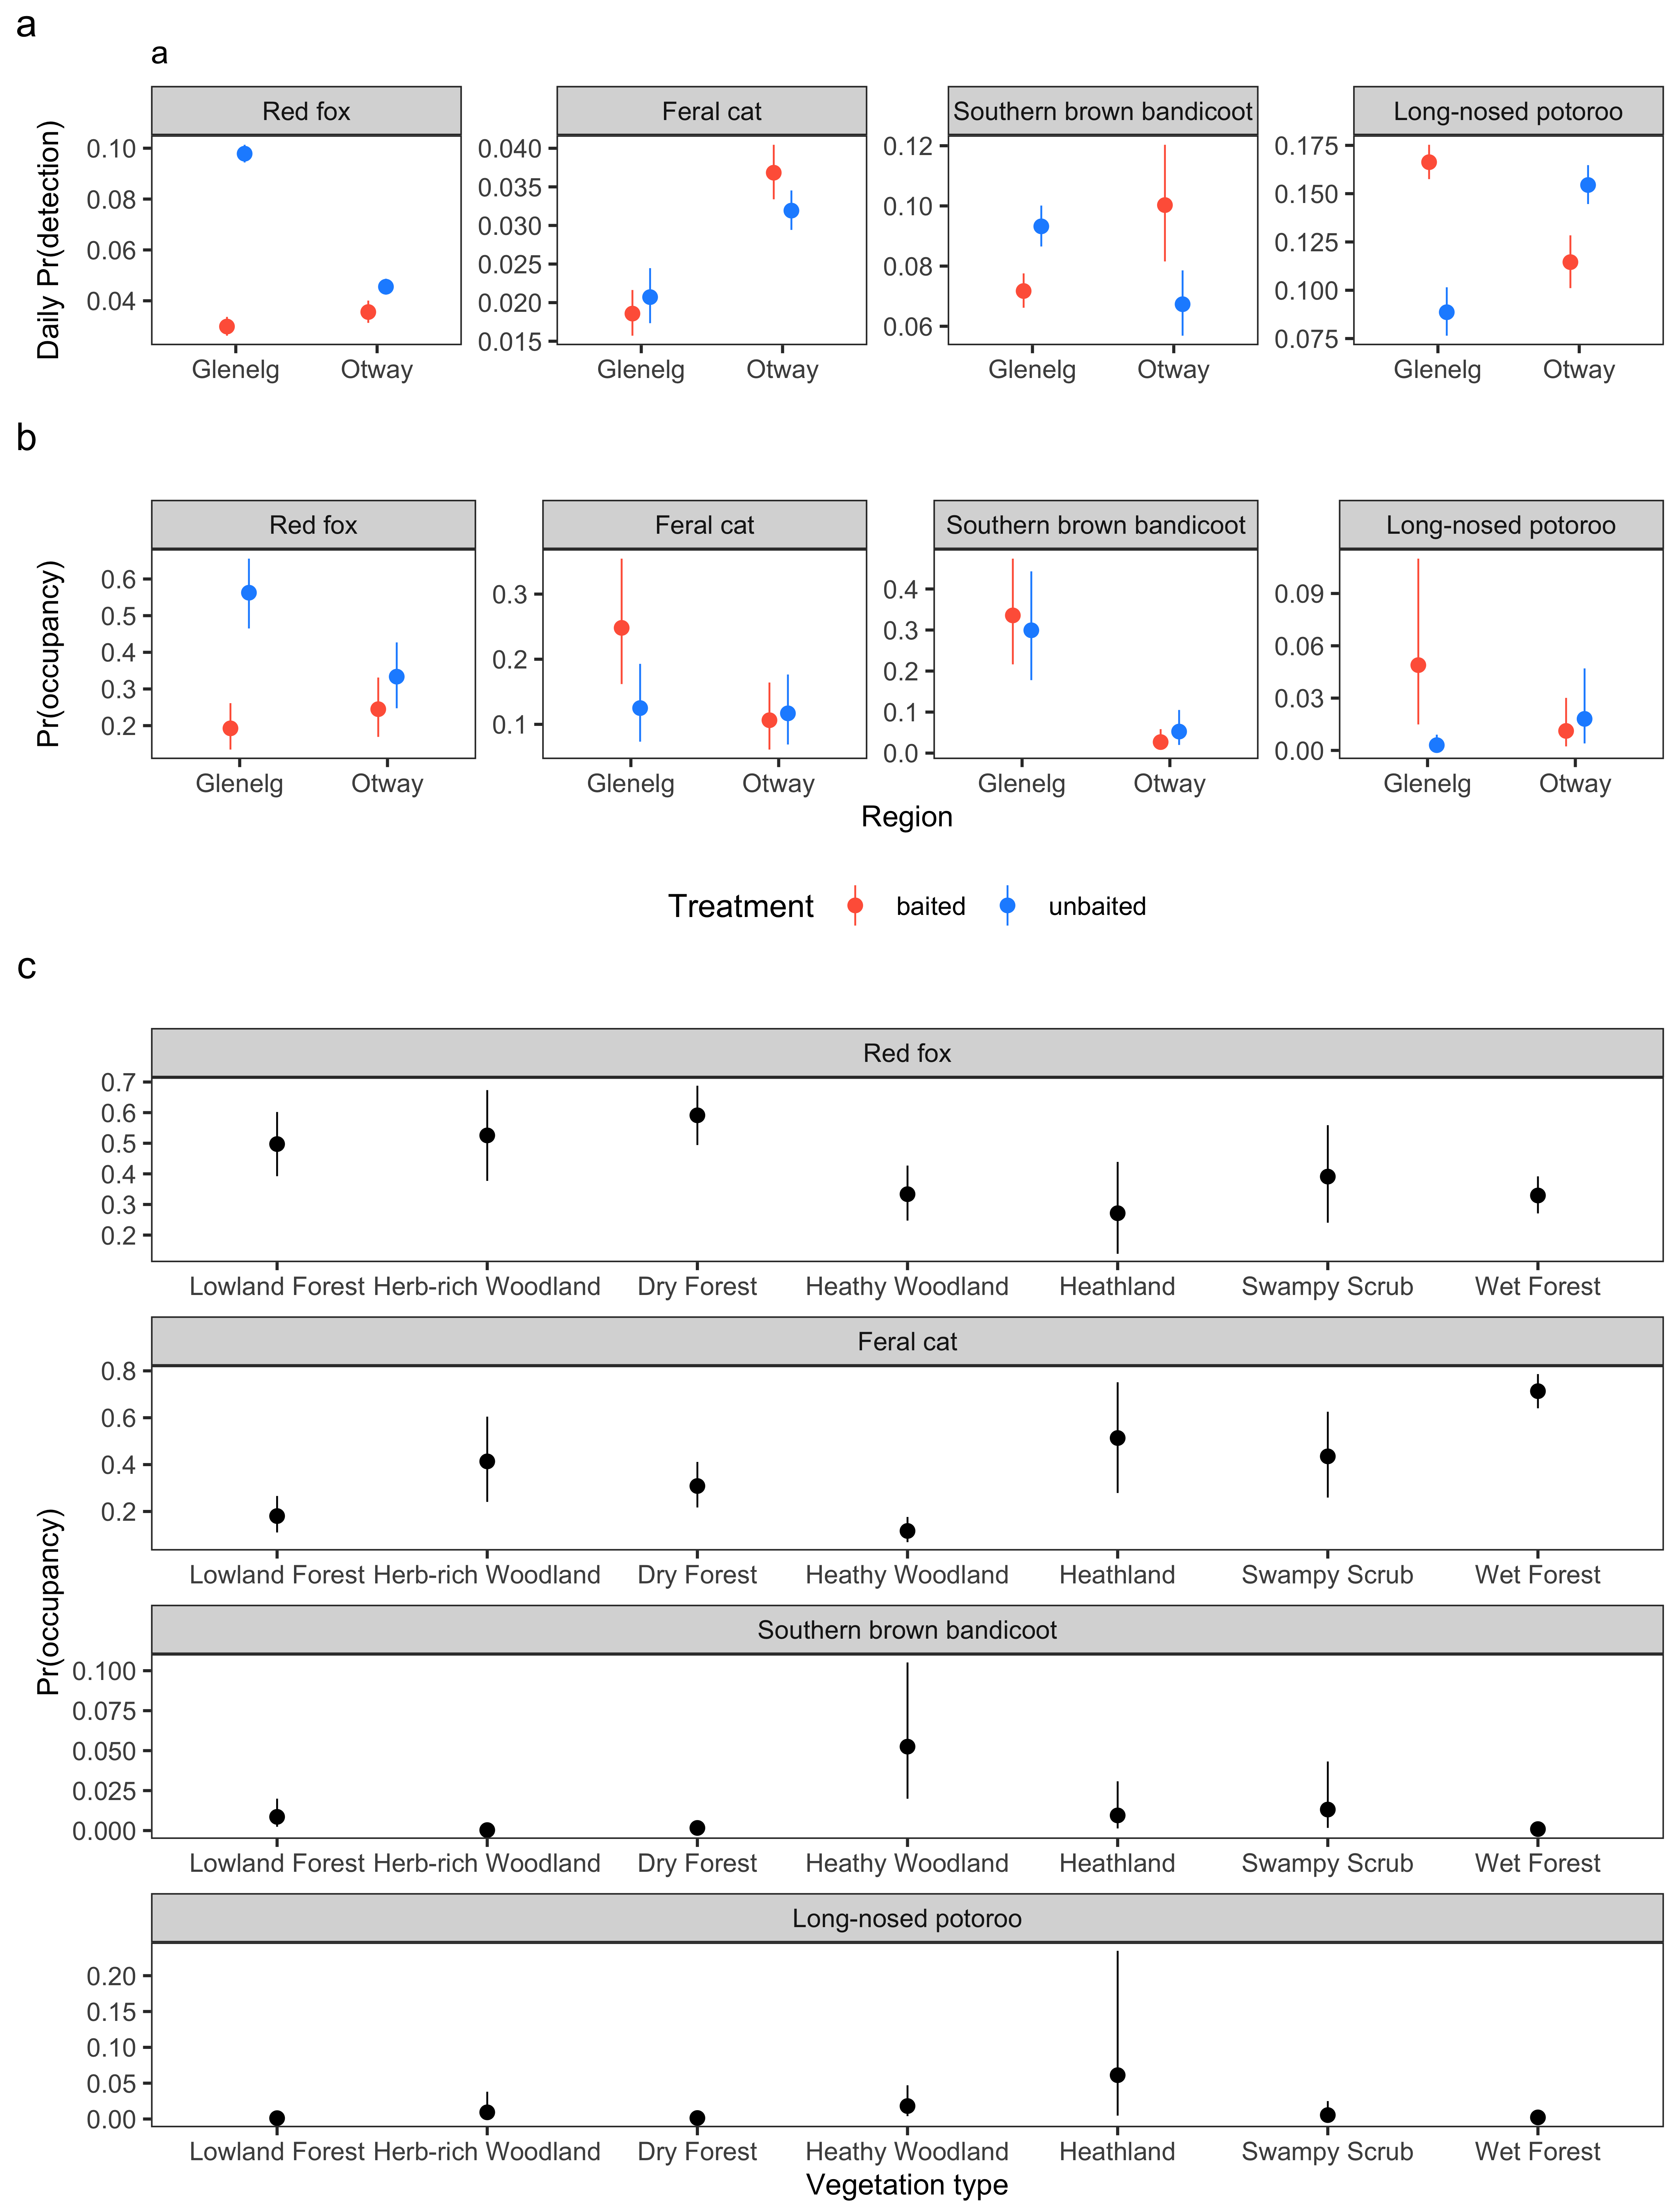
\includegraphics[width=1\linewidth]{figure/occ_det_ubms} 

}

\caption{Outputs from Bayesian occupancy-detection for each study species. Daily detection probabilities (a) and occupancy estimates (b) in landscapes with fox control (red) and without fox control (blue) in the Glenelg region and Otway Ranges, south-west Victoria, Australia (with Heathy Woodlands as a reference level). Fox control had occurred in The Glenelg region for 8 - 13 years and was monitored with a control-impact design. The Otway Ranges was monitored using a before-after-control-impact experimental design; surveyed approximately 1 year prior and 2 years following the commencement of fox-baiting. Occupancy was also modelled as a function of vegetation type (Ecological Vegetation Class groups; c). Error bars represent 95\% Bayesian credible intervals.}\label{fig:occ-det}
\end{figure}
\newpage
\begin{figure}

{\centering 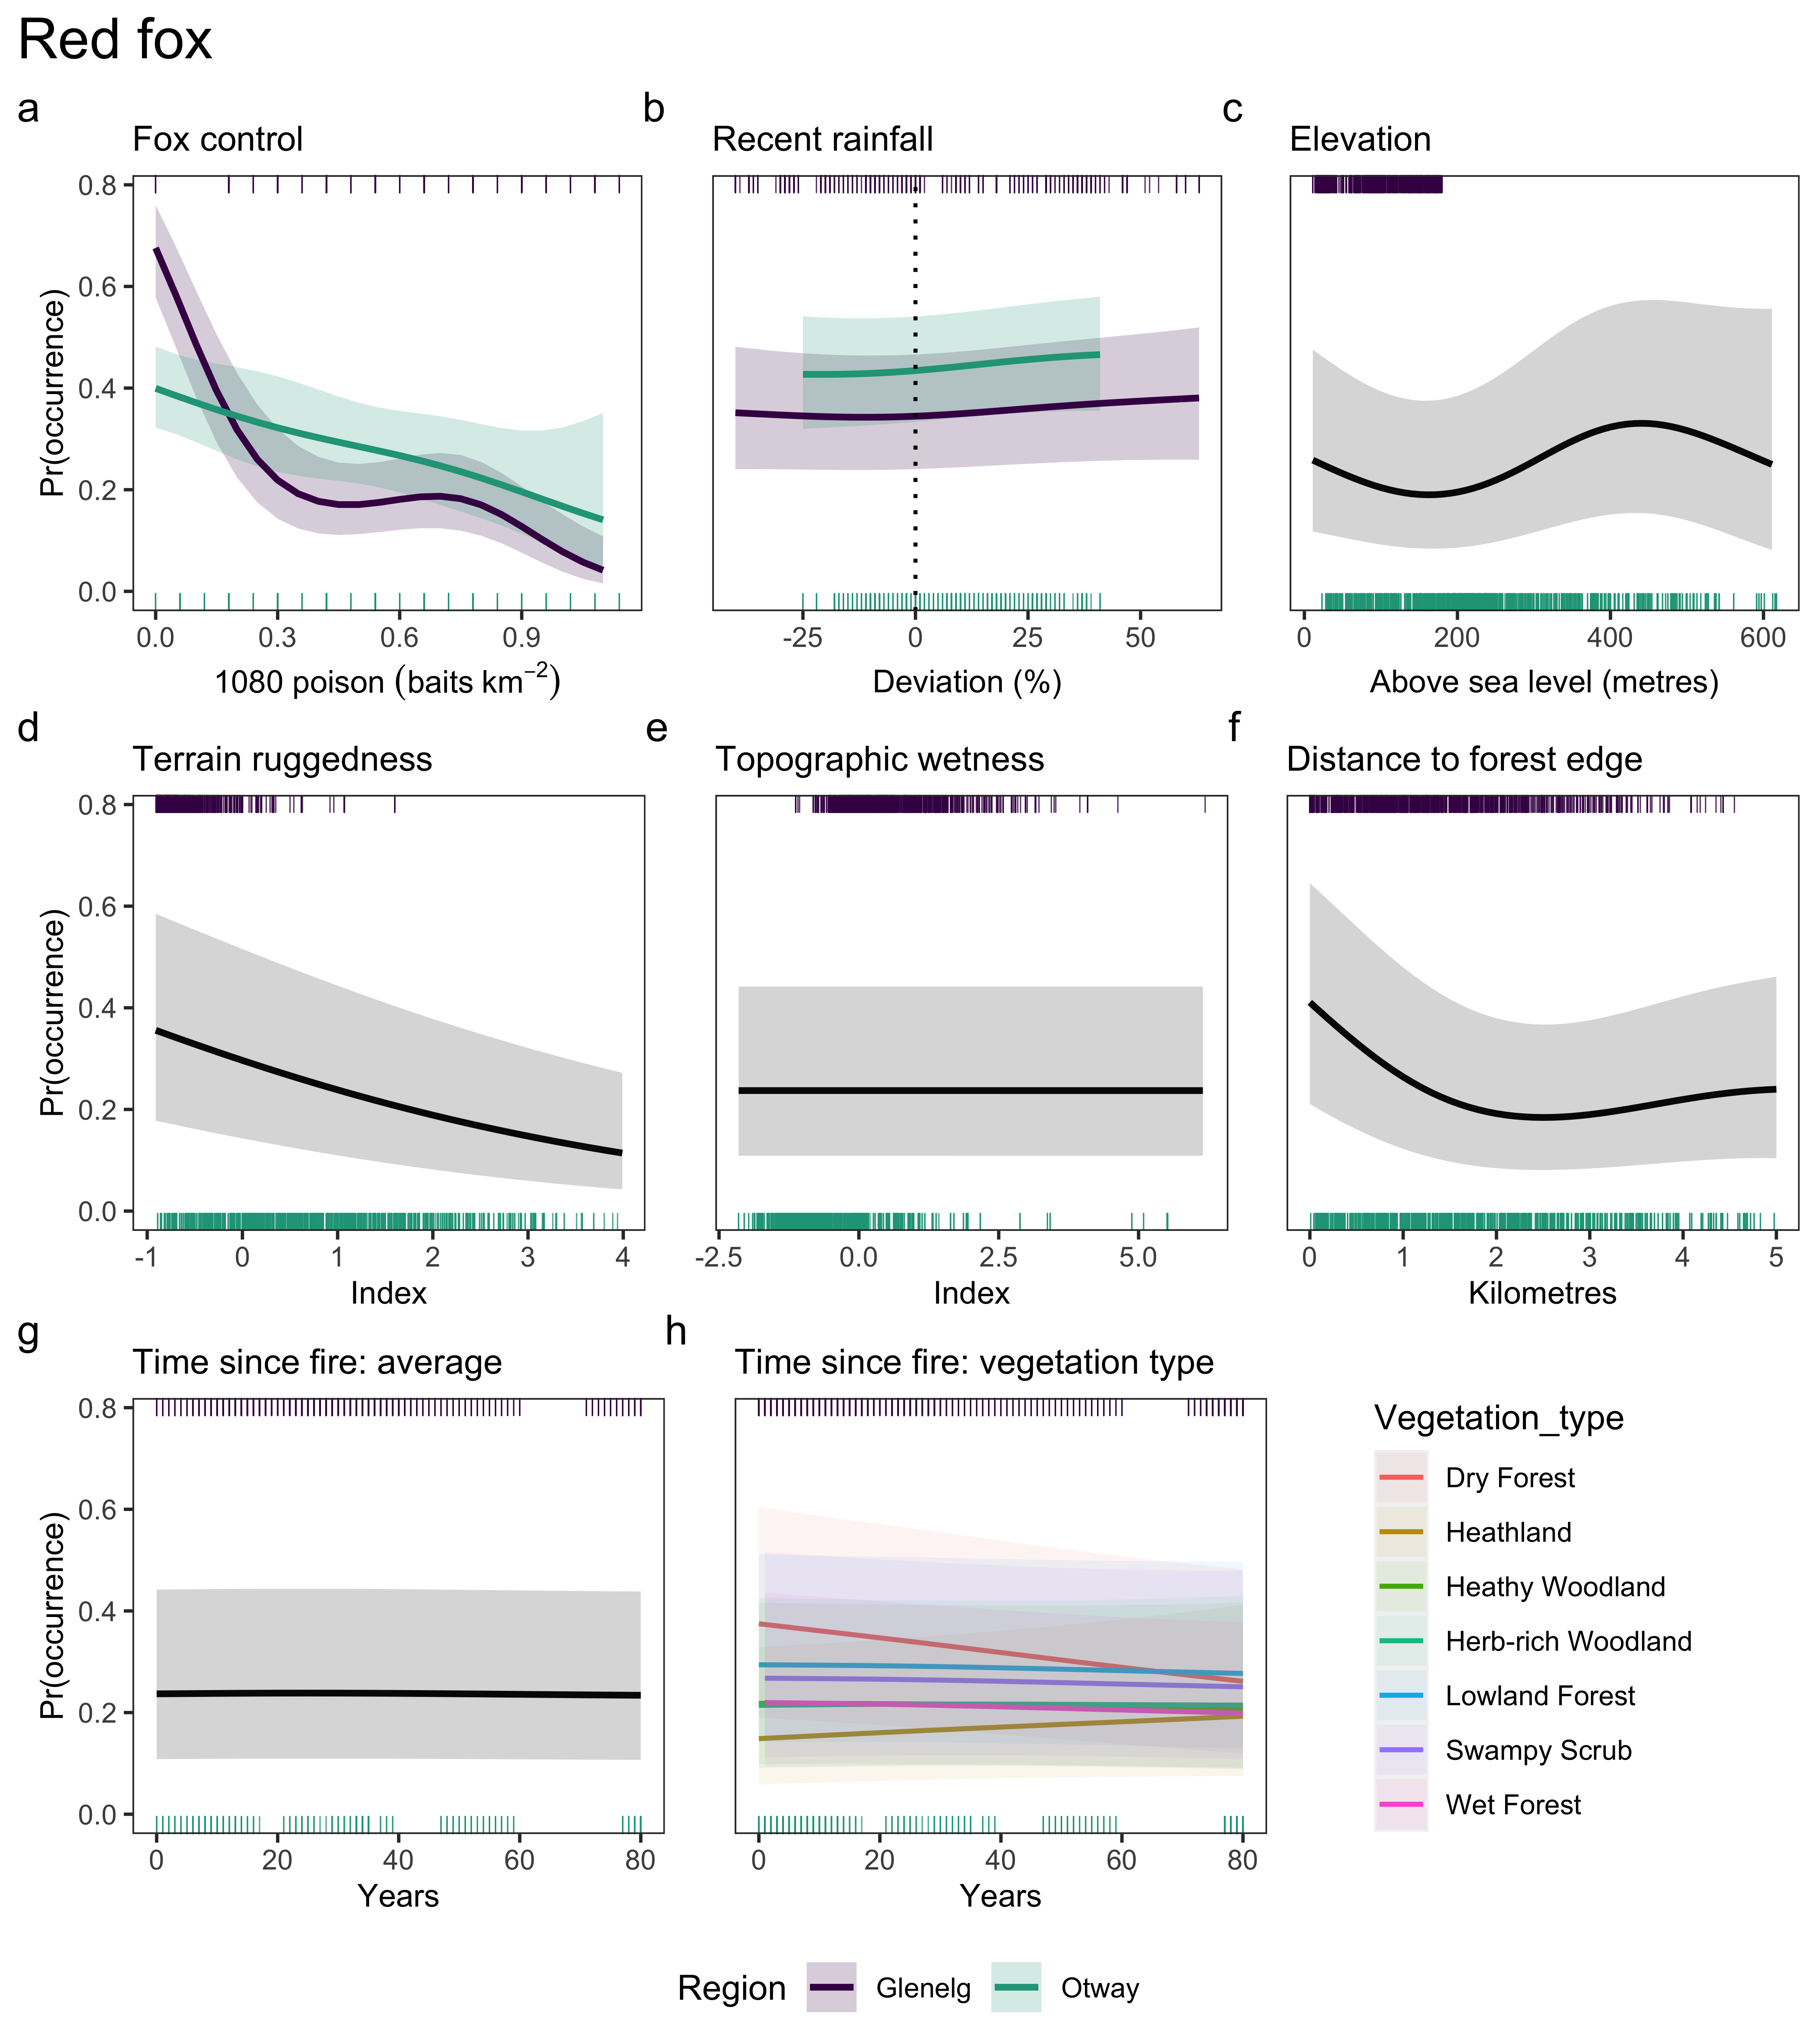
\includegraphics[width=1\linewidth]{figure/gams_fox} 

}

\caption{Generalised additive model estimates of the effect of each explanatory variable (columns) on red fox \textit{Vulpes vulpes} occurrence. Shaded bands indicate 95\% confidence intervals.}\label{fig:gams-occ-fox}
\end{figure}
\newpage
\begin{figure}

{\centering 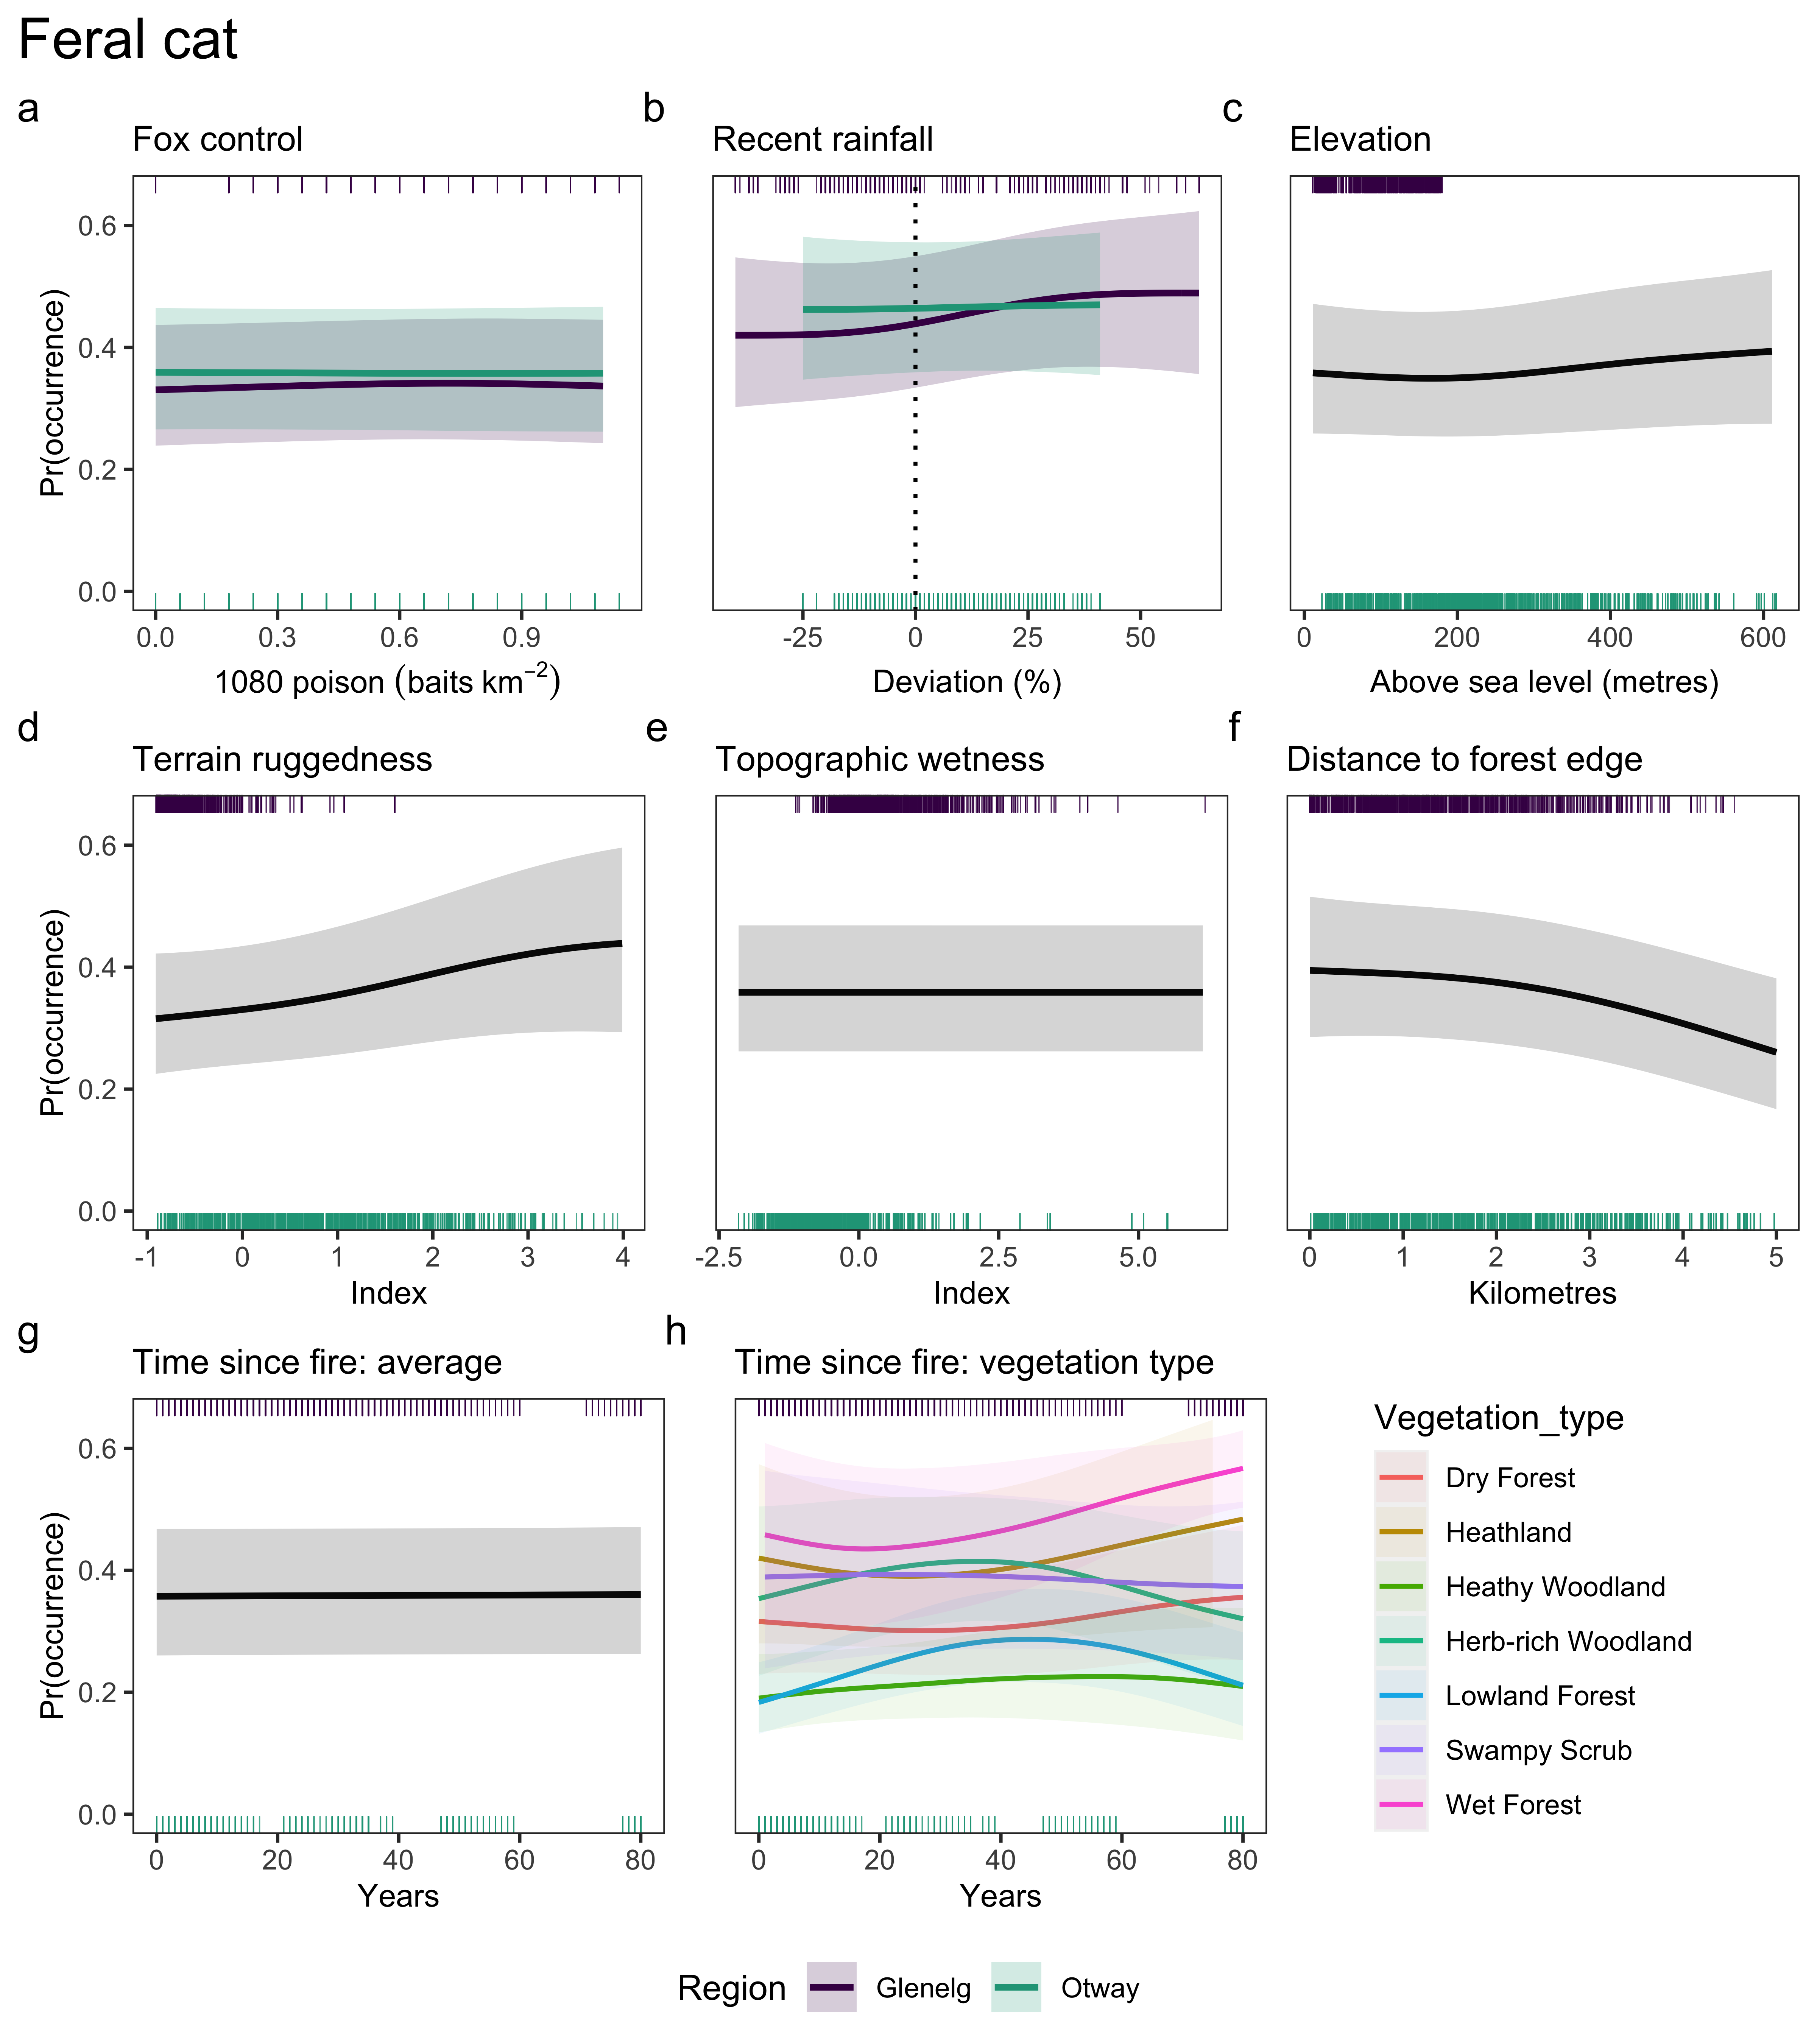
\includegraphics[width=1\linewidth]{figure/gams_cat} 

}

\caption{Generalised additive model estimates of the effect of each explanatory variable (columns) on feral cat \textit{Felis catus} occurrence. Shaded bands indicate 95\% confidence intervals.}\label{fig:gams-occ-cat}
\end{figure}
\newpage
\begin{figure}

{\centering 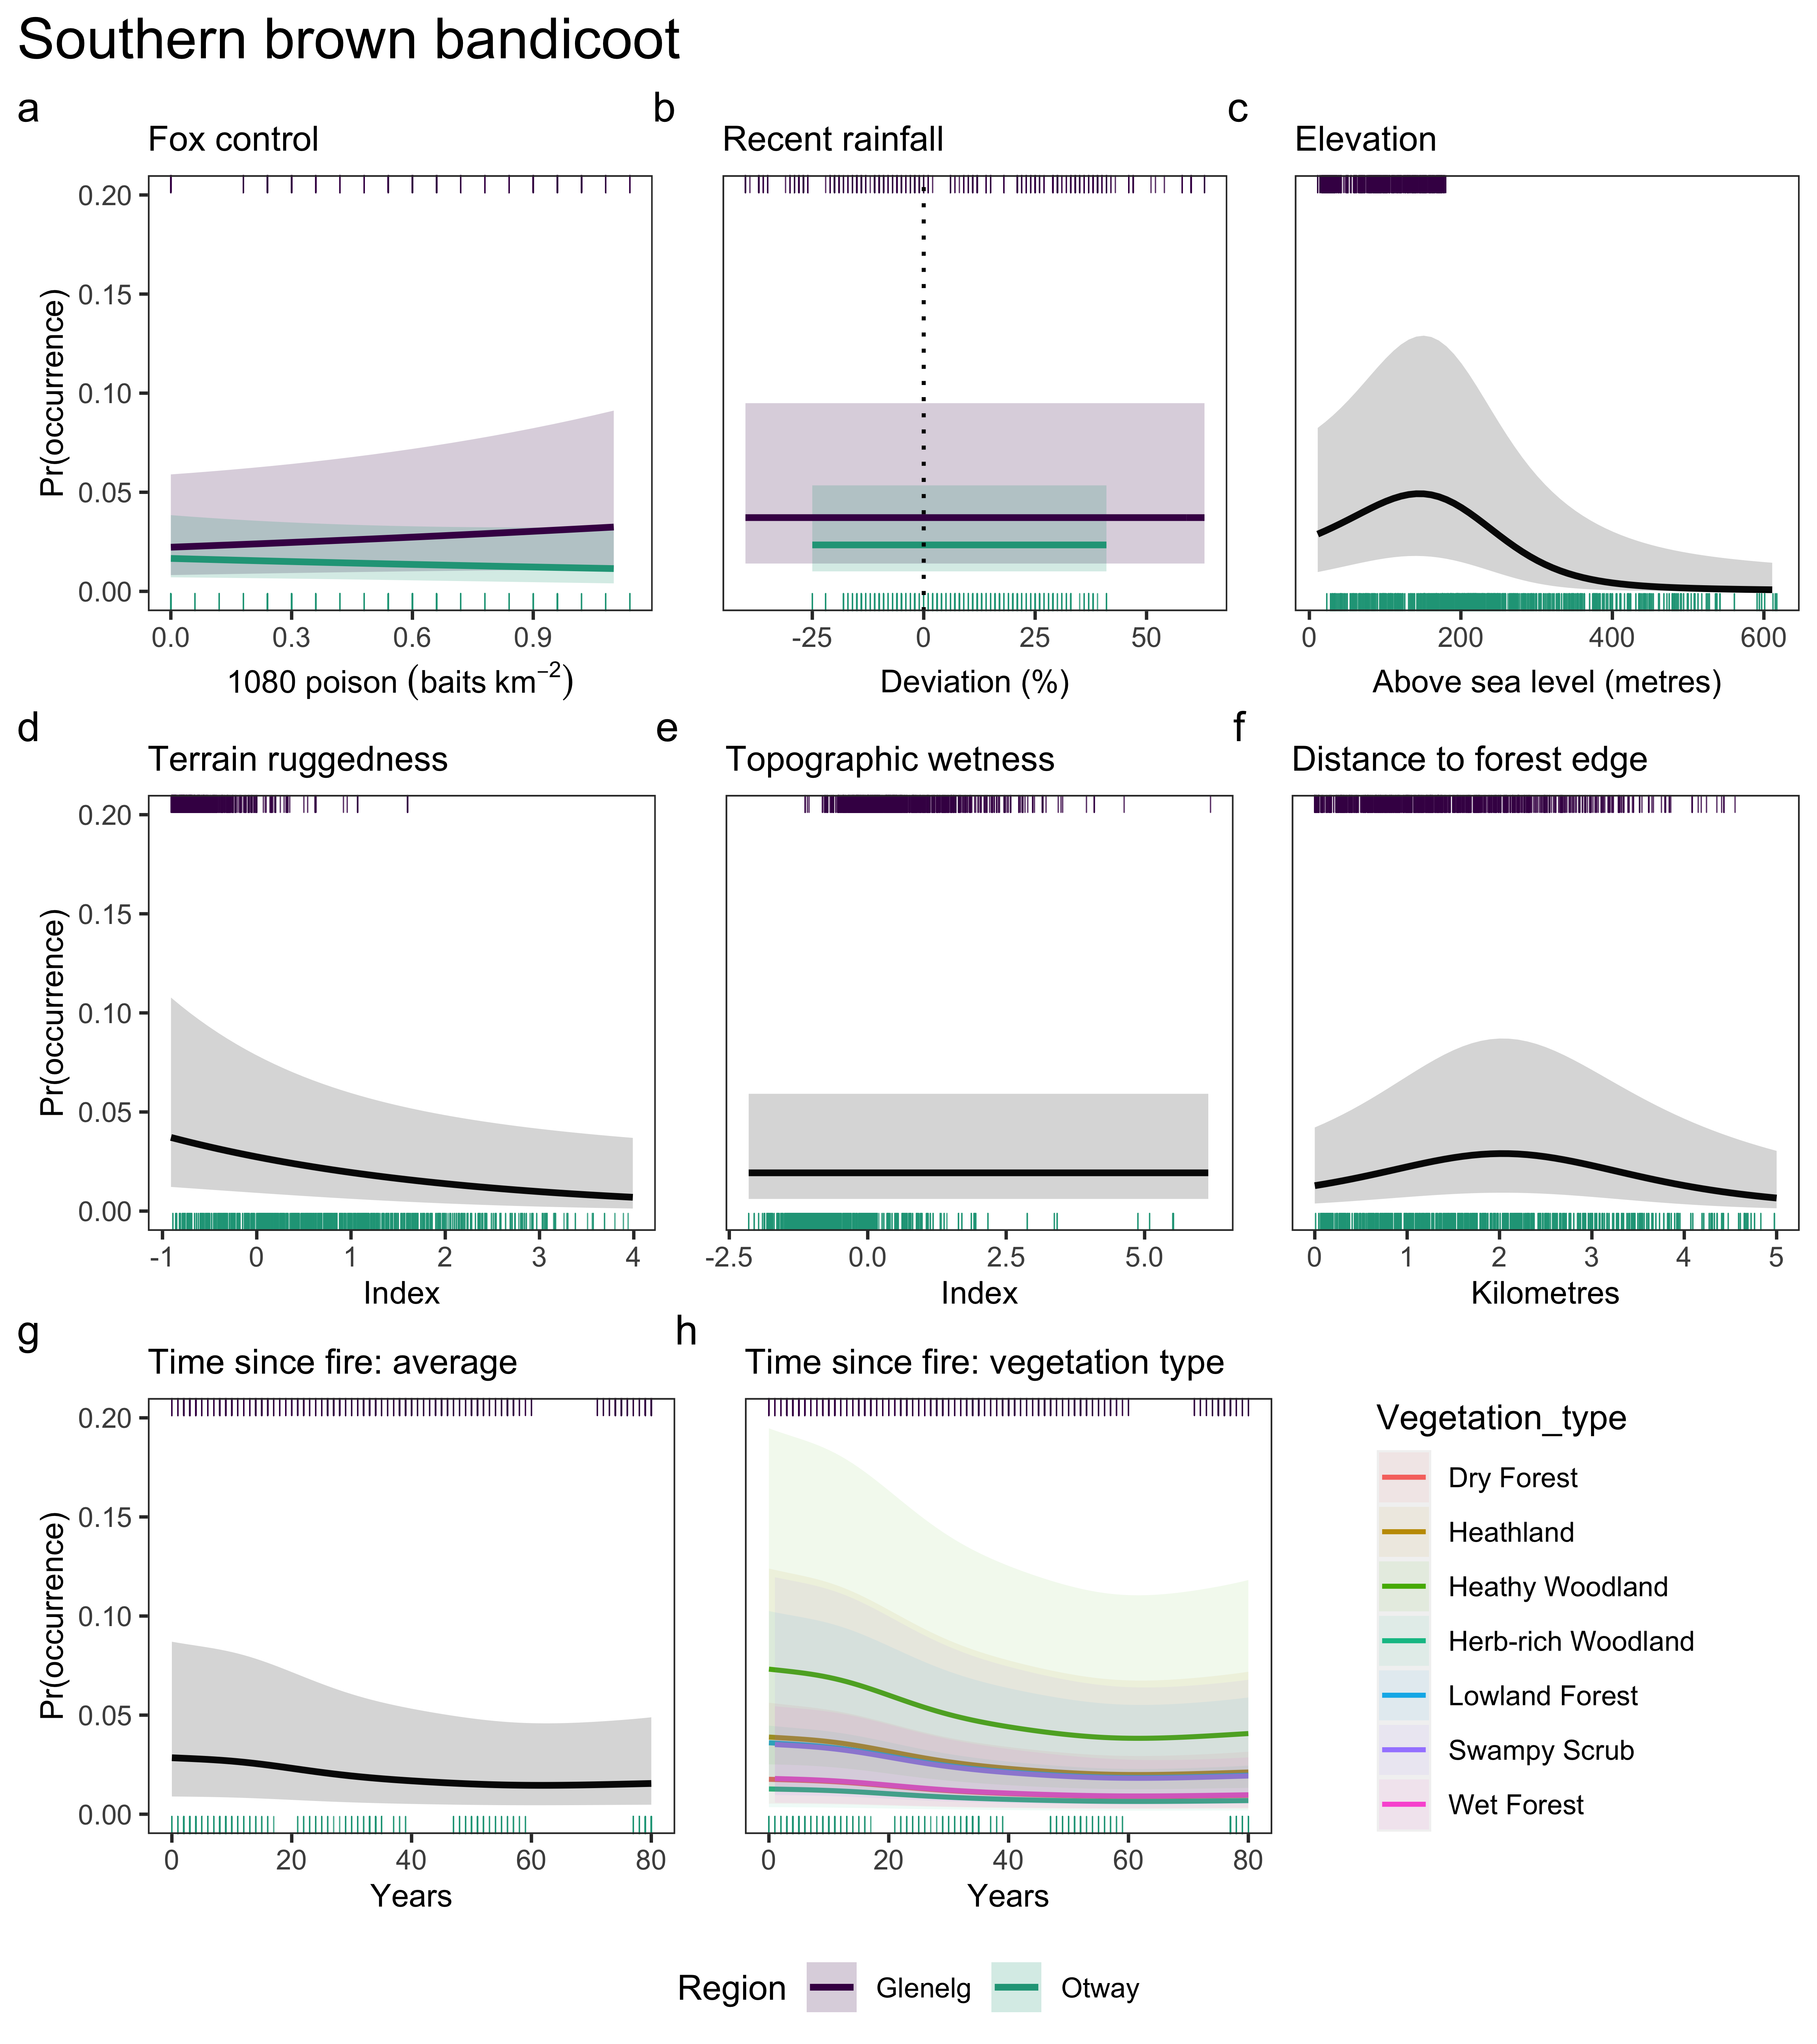
\includegraphics[width=1\linewidth]{figure/gams_sbb} 

}

\caption{Generalised additive model estimates of the effect of each explanatory variable (columns) on southern brown bandicoot \textit{Isoodon obesulus} occurrence. Shaded bands indicate 95\% confidence intervals.}\label{fig:gams-occ-sbb}
\end{figure}
\newpage
\begin{figure}

{\centering 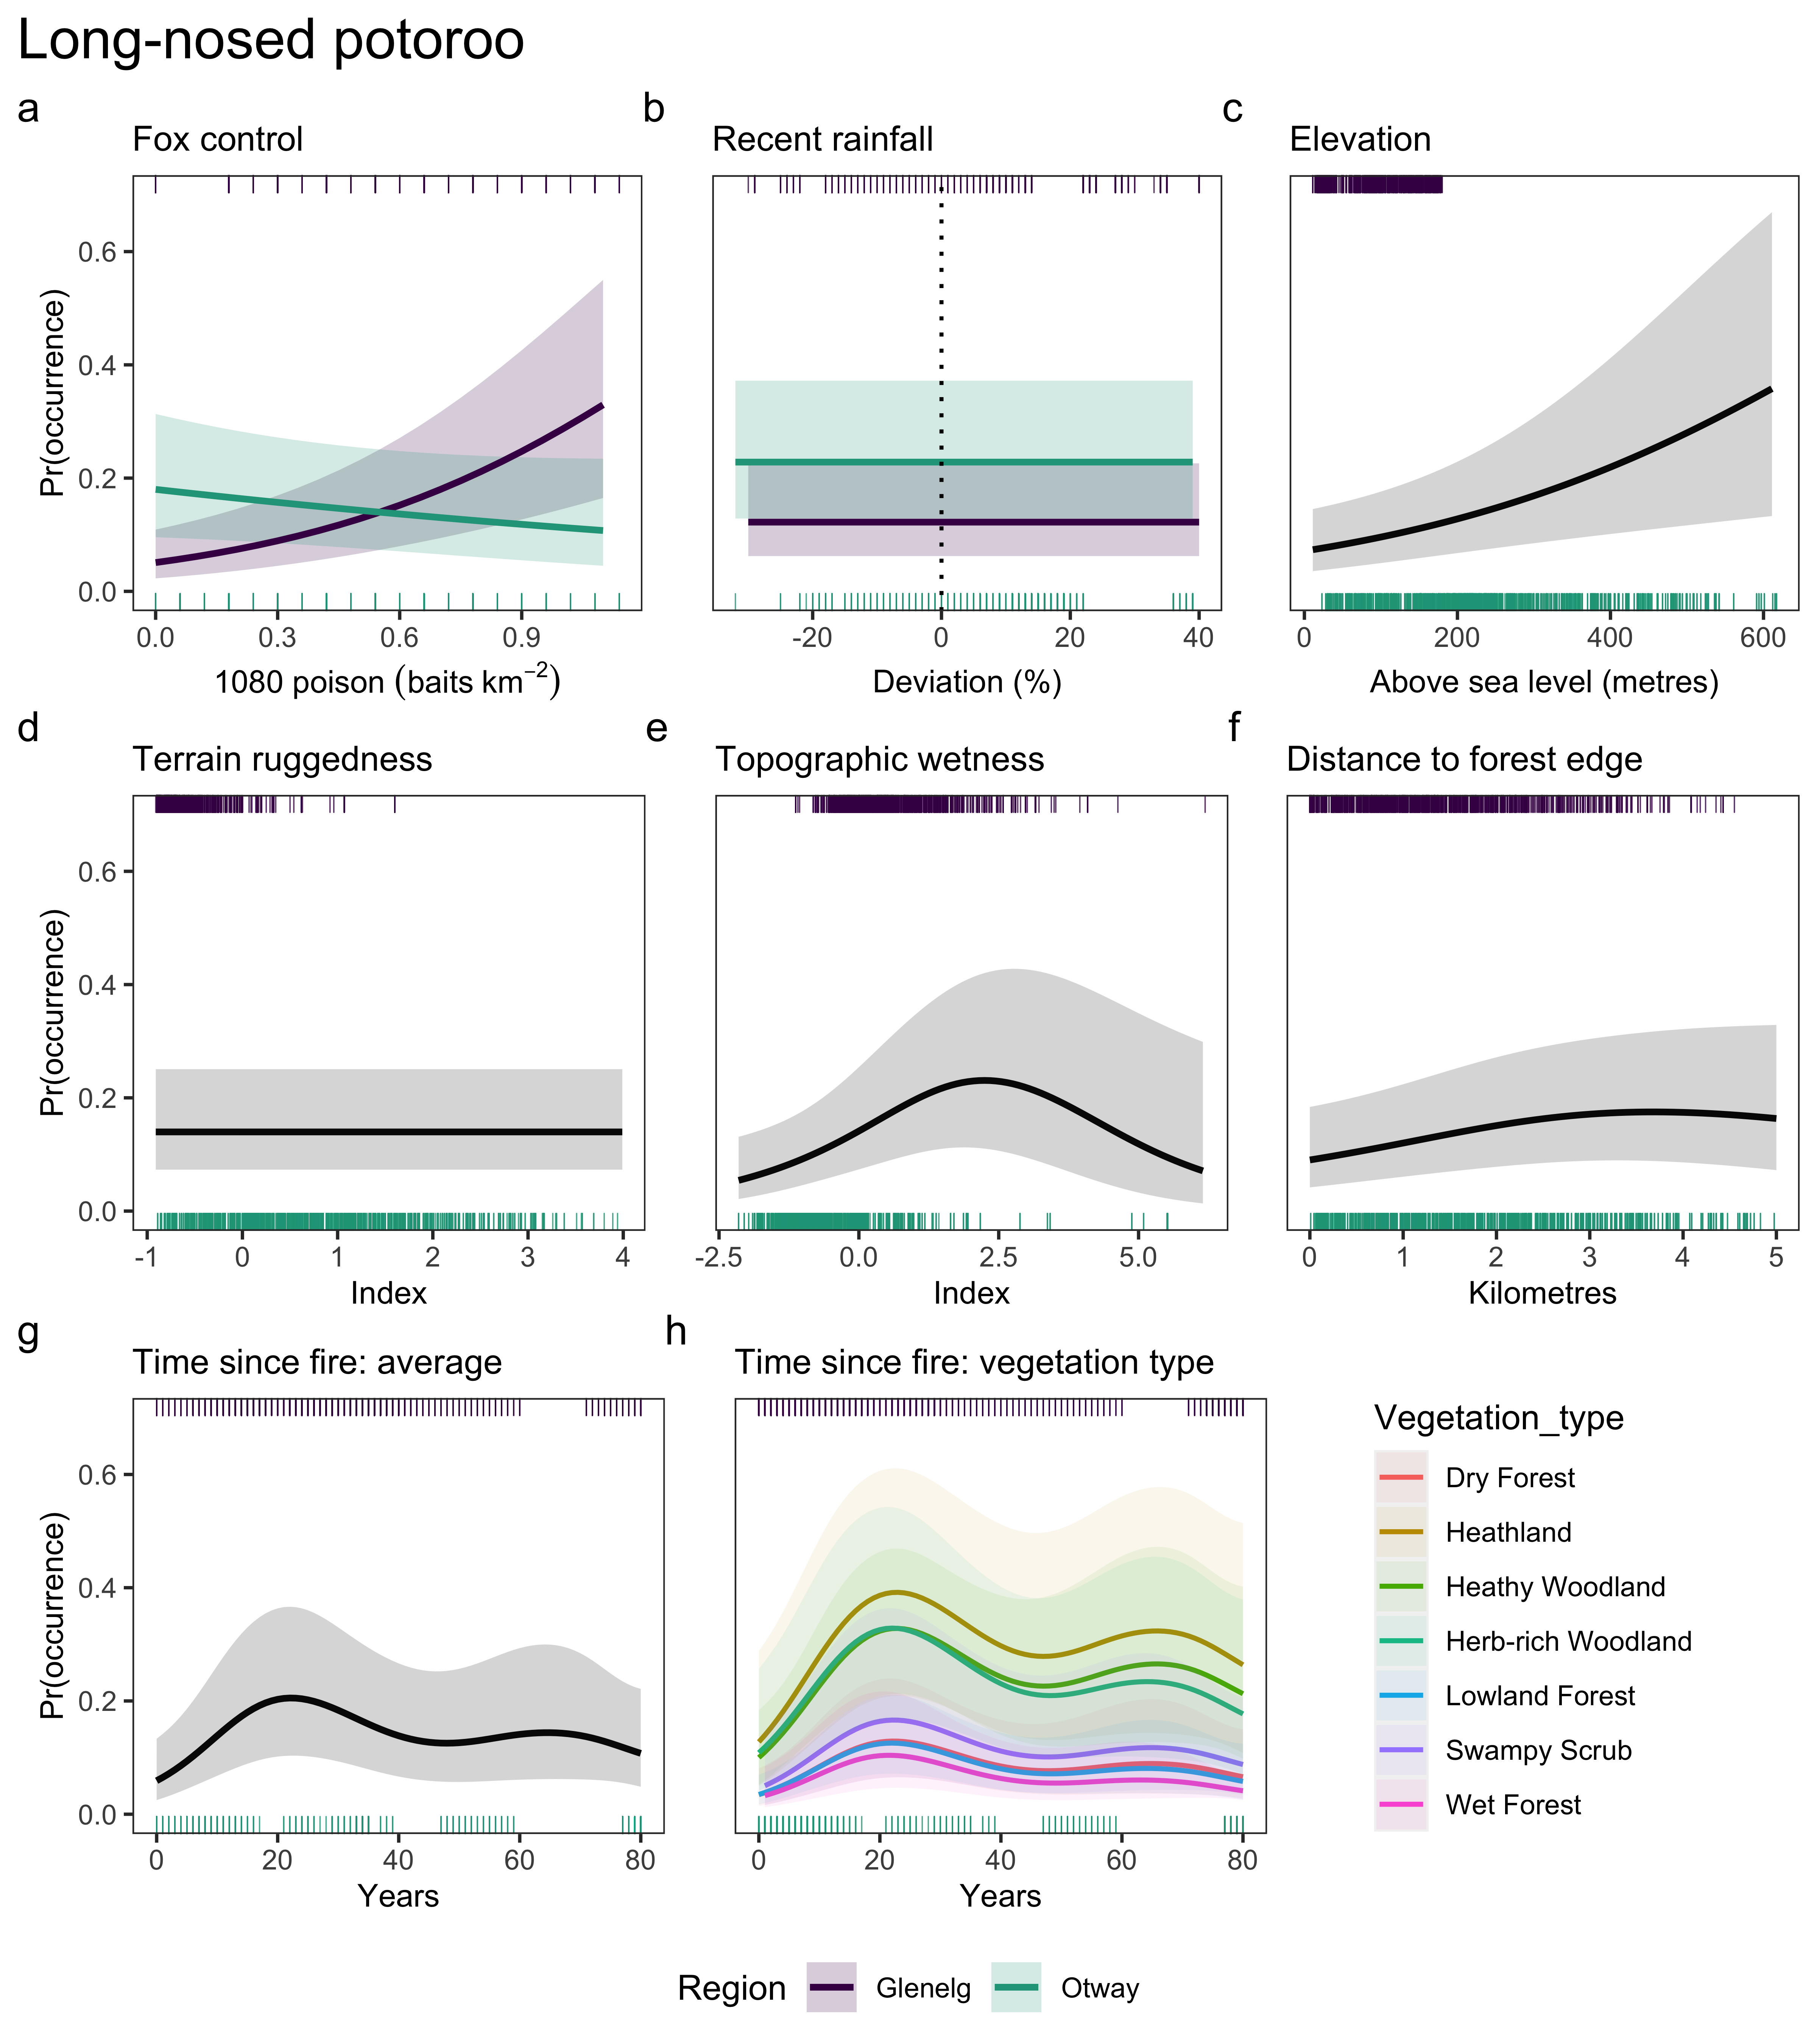
\includegraphics[width=1\linewidth]{figure/gams_lnp} 

}

\caption{Generalised additive model estimates of the effect of each explanatory variable (columns) on long-nosed potoroo \textit{Potorous tridactylus} occurrence. Shaded bands indicate 95\% confidence intervals.}\label{fig:gams-occ-lnp}
\end{figure}
\newpage

\hypertarget{discussion-1}{%
\section{Discussion}\label{discussion-1}}

Here we found that consistent and long-term lethal control can reduce a widespread invasive apex predator (fox) to a near-zero occurrence probability--and importantly--increase the occurrence probability of a threatened prey species (LNP) by more than 6-fold (Fig. \ref{fig:gams-occ-fox}a; Fig. \ref{fig:gams-occ-lnp}a). However, prey responses to predator suppression are not universal (Salo \emph{et al.} 2010; Hunter \emph{et al.} 2018; Duncan \emph{et al.} 2020). Despite initial signs of improvement in the Glenelg region (Robley \emph{et al.} 2014), SBB occupancy was mostly unaffected by fox control in our study (Fig. \ref{fig:occ-det}b; Fig. \ref{fig:gams-occ-lnp}a). This may have been because feral cat occupancy was twice as high in the landscapes with fox control relative to those without in the Glenelg region (Fig. \ref{fig:occ-det}b), potentially signalling mesopredator release. In another region where fox control recently commenced with less frequent baiting, foxes were suppressed to a lesser extent and neither threatened prey species showed signs of improvement (Fig. \ref{fig:occ-det}b; Fig. \ref{fig:gams-occ-fox}a; Fig. \ref{fig:gams-occ-sbb}a; Fig. \ref{fig:gams-occ-lnp}a). Our study demonstrates that lethal invasive predator control can be a highly effective conservation strategy, but only for some species and when sustained continuously over the long-term.

The Glenelg Ark program has continuously controlled foxes across approximately 100 000 ha of public land since 2005 (Robley \emph{et al.} 2014) and is one of the few fox control programs in Australia to demonstrate a sustained reduction in fox occupancy (see also Stobo-Wilson \emph{et al.} 2020a). A reduction in fox occupancy is a strong sign of management effectiveness because it means prey are less exposed to the threat of predation. Our study provides empirical evidence that the effectiveness of fox control from poison-baiting programs depends on the density of poison-baits deployed (Fig. \ref{fig:gams-occ-fox}a). This has only previously been inferred by comparing fox baiting programs across different regions (where fox ecology, environmental conditions and study designs differ). The densities of poison-baits in our study regions (maximum 1.14 baits km\textsuperscript{-2}) were far below the recommended 5 - 10 baits km\textsuperscript{-2} (mostly derived from studies in arid and semi-arid regions; Saunders \& McLeod 2007), but nonetheless effective at fox suppression in the Glenelg region (Fig. \ref{fig:occ-det}b). Controlling foxes with 0.1 - 0.3 baits km\textsuperscript{-2} was particularly effective in the Glenelg region, reducing fox occurrence by up to four-fold; higher poison-bait densities suppressed fox occurrence to a lesser extent (Fig. \ref{fig:gams-occ-fox}a). Increased bait caching at high bait densities may explain why fox suppression tapered off, which is likely to result in a sublethal dose when eventually consumed and potential bait aversion (Saunders \& McLeod 2007). Nonetheless, benefits to threatened native prey is the best metric of fox control effectiveness. The probability of LNP occurrence increased linearly with poison-bait density in the Glenelg region (Fig. \ref{fig:gams-occ-lnp}a), confirming that high fox control effort leads to improved conservation outcomes.

We slightly underestimated the effect of bait density across both regions because the models assumed all bait-stations were constantly active, despite some bait-replacements being missed due to accessibility issues following wet weather events or because of more pressing management concerns (namely wildfire). We more strongly underestimated the effect of bait density in the Otway Ranges because we also did not account for the near six month pause in bait replacement in 2018. We also expect fox-baits to be less effective in the Otway Ranges than the Glenelg region due to the high average rainfall which more quickly degrades the poison (Saunders \emph{et al.} 2000; Gentle \emph{et al.} 2007). Nonetheless, fox occupancy in the Otway Ranges was still negatively associated with fox-bait density (Fig. \ref{fig:gams-occ-fox}a), suggesting that intensified and sustained fox control is likely to be effective in that region. Future research will benefit from accounting for the role of environmental conditions and prey availability on baiting effectiveness (Saunders \& McLeod 2007; Carter \& Luck 2013), as well as interference with baits by non-target species (Fairbridge \emph{et al.} 2000; Glen \& Dickman 2003; Marlow \emph{et al.} 2015b).

Evidence that fox control caused a mesopredator release of feral cats in terms of detectability and occupancy was mixed. Cat detectability increased with fox control in the Otway Ranges, and cat occupancy was higher in sites with fox control in the Glenelg region (Fig. \ref{fig:occ-det}a:b). However, cat occurrence did not change across gradients of poison-bait density in either region (GAM; Fig. \ref{fig:gams-occ-cat}a). Cat detectability in the Glenelg region was very low (Fig. \ref{fig:occ-det}a), and so the model assumption of perfect detection in the cat GAM was likely problematic. This result could also signal that cats respond to fox suppression at the landscape level rather than at finer spatial scale. In addition, potential changes in population density and behaviour following mesopredator release (Brashares \emph{et al.} 2010), such as cats reducing their ranging behaviour following fox control (as found by Molsher \emph{et al.} 2017), could skew inference around occupancy estimates (Efford \& Dawson 2012; McCarthy \emph{et al.} 2013; Neilson \emph{et al.} 2018; Stewart \emph{et al.} 2018; Broadley \emph{et al.} 2019). Cats had weak associations with most explanatory variables, the poorest detection rates and worst model fits of our study species, further highlighting the challenges of monitoring this elusive, generalist predator (Fisher \emph{et al.} 2015; Stokeld \emph{et al.} 2015; Algar \emph{et al.} 2020).

In the Glenelg region, LNP--but not SBB--occupancy improved with fox control (Fig. \ref{fig:occ-det}b). Monitoring prey occupancy to measure the effectiveness of predator control rests on the assumption that there is suitable habitat for prey to expand into. While SBBs had a narrower distribution relative to LNPs across our study regions (largely absent from the wet forests), there was 34 heathy woodland sites in the Glenelg region where they were never observed (from 196 camera-trap deployments), suggesting there was suitable habitat for them to colonise. There may have been a variable which precluded SBB presence at these 34 sites, most likely habitat structure (Swan \emph{et al.} 2015), although Smith (2013) found no association between habitat structure and SBB occupancy in the 240 Glenelg Ark monitoring sites. Instead, the different prey responses in our study most likely reflect the relative vulnerability of these species to fox and cat predation: LNPs (and other small macropods) appear more strongly limited by fox predation, whereas SBBs tend to be more closely associated with cat populations (Arthur \emph{et al.} 2012; Hunter \emph{et al.} 2018) and so may have experienced negative consequences from higher cat occupancy in landscape with fox control. This would also help explain why SBB occupancy was highest in heathy woodlands, where cat occupancy is lowest (Fig. \ref{fig:occ-det}c). Formally testing whether invasive predator occupancy impacts the probability of prey occupancy using multispecies models (Rota \emph{et al.} 2016) is a priority for future research.

In the Otway Ranges, fox control did not improve SBB or LNP occupancy (Fig. \ref{fig:occ-det}b; Fig. \ref{fig:gams-occ-sbb}a); Fig. \ref{fig:gams-occ-lnp}a). This is unsurprising given fox suppression in the Otway Ranges was weak, likely because fox control had only recently commenced and bait replacements were inconsistent (relative to the Glenelg region). Despite the high fecundity of these prey species, two years was may have been insufficient time to measure an effect of fox control on prey occupancy. Additionally, we averaged fox control effects over a 0 - 2 year time period in the Otway ranges, although, our findings concur with those of Robley \emph{et al.} (2019), who estimated annual occupancy probabilities using a more traditional BACI analysis with a subset of this data. Fortunately, the ongoing broadscale monitoring of the Otway Ark fox control program and other local initiatives will shed light on occupancy trends over time.

Fire can have long-term impacts on the occurrence of small-medium sized native mammals (Claridge \& Barry 2000; Monamy \& Fox 2000; Arthur \emph{et al.} 2012). Previously, Smith (2013) found extinction probabilities for both LNPs and SBB's to be high for up to 18 months post-fire. Here we found that, for individuals which persisted through the initial burn period, LNP occurrence improved and peaked in 20 years post-fire (Fig. \ref{fig:gams-occ-lnp}g). However, seemingly contrary to Smith (2013), SBB occurrence declined with increasing TSF (Fig. \ref{fig:gams-occ-sbb}g). Given the uncertainty around our estimates and importance for managers implementing prescribed fire, further research is required to clarify and understand the mechanisms behind these responses to fire. A key question remaining in particular is whether fox control impacts prey responses to fire in the short and long-term.

Our work adds to the small body of evidence that fire patterns can impact the occurrence of predators (Geary \emph{et al.} 2020a). While there is now considerable research which has demonstrated that invasive predator impacts are heightened in recently burnt areas (Meek \& Saunders 2000; Green \& Sanecki 2006; McGregor \emph{et al.} 2014, 2016; Leahy \emph{et al.} 2016; Hradsky \emph{et al.} 2017a, c), we have a comparitively poor understanding of how long-term fire patterns impact invasive predators (reviewed in Hradsky 2020). Similar to previous studies, we found no average response to TSF for foxes or cats, however, both predators had varying responses to TSF across vegetation types (Fig. \ref{fig:gams-occ-fox}g:h; Fig. \ref{fig:gams-occ-cat}g:h;). This supports the `dynamic vegetation' hypothesis (Nimmo \emph{et al.} 2014); the first evidence of this kind for predators (although, uncertainty around these estimates was high). Studies often merge similar vegetation types due to some groups having small sample sizes, however, we found no clear way of grouping vegetation types that was relevant to multiple species. Our hierarchical specification of the TSF and vegetation type interaction was powerful in this regard as it allowed separate responses for each vegetation type, while sharing information across vegetation types (and providing confidence that there was data to back-up differently shaped responses given the penalisation to the average response; Pedersen \emph{et al.} 2019).

Accounting for other drivers of species in models that estimate responses to management is critical, but not often undertaken. For example, unexpected declines and local extinctions of small-medium sized mammals have occurred following 40 years of fox control in south-west Western Australia (thought to be the result of a mesopredator release of cats; Wayne \emph{et al.} 2017a), but the Intergovernmental Panel on Climate Change has identified this region as a `drying hotspot' (Kala \emph{et al.} 2021) and there are strong concerns around the intensity of prescribed fire operations (e.g., Bennett \& Edwards 2021), offering alternative explanations for prey declines. Mammal communities have also collapsed following long-term fox-control in Booderee National Park (Lindenmayer \emph{et al.} 2018), although a severe wildlife burnt through approximately half the region in the same year fox control commenced (leaving greater than 73\% of park burnt within the last decade; Foster \emph{et al.} 2017). Similarly, recent fire events have, by chance, been skewed towards the baited landscapes of the Glenelg region since fox control began, with the majority of long-unburnt vegetation occurring in unbaited landscapes (Fig. \ref{fig:veg-tsf-violin}). We were able to compensate for this confounding by also including an additional 424 sites in the Glenelg region, as well as the Otway Ranges datasets--providing a wider range of fire history patterns in each vegetation type with and without fox control (Fig. \ref{fig:veg-tsf-violin}). Our study demonstrates the value of bringing together multiple smaller datasets to compare management effectiveness.

Occurrence models are powerful tools to predict species distributions but less useful for explaining fine-scale site-use for wide-ranging, generalist species in continuous habitat (Efford \& Dawson 2012; Guillera-Arroita \emph{et al.} 2015). Despite our large dataset, uncertainty for most explanatory variables was high. Our study offers little additional clarity about the `natural' drivers of occurrence for invasive predators and medium-sized mammalian prey within their distributions other than clarifying the importance of broad vegetation type. While we did seek to provide inference on drivers these species, our key aim was to account for confounding variables while testing fox control effects. Nevertheless, testing the predictive performance of distribution models for these species, in particular whether region-specific or across-region models predict more accurately will aid the management of these species.

Fox control is a major expenditure of Australian conservation and agricultural programs (approximately AUD 16 million annually; McLeod \& Norris 2004). It is critical to ensure cost-effectiveness from both a monetary and ethical standpoint. Here we demonstrate that effectiveness in terms of fox suppression is a function of control effort, although evidence of benefits to native prey species were mixed in this study. Prey may not benefit from predator control if mesopredator release of other invasive predators occurs or if prey are constrained by other factors such as lack of suitable habitat. Species vulnerable to fox predation are also sensitive to fire-induced changes in habitat structure (Woinarski \emph{et al.} 2015), and so integrating conservation strategies which consider habitat and invasive predator management in concert is a future priority. Our work highlights the importance of fine-scale monitoring, considering multiple drivers and tailoring conservation strategies to local contexts.

\hypertarget{density}{%
\chapter{Quantifying mesopredator release: lethal control of an invasive apex predator alters feral cat density and detectability}\label{density}}

\hypertarget{abstract-2}{%
\section*{Abstract}\label{abstract-2}}
\addcontentsline{toc}{section}{Abstract}
\begin{enumerate}
\def\labelenumi{\arabic{enumi}.}
\item
  The mesopredator release hypothesis predicts that subordinate predator density will increase as apex predators decline. Persistent debate around mesopredator release in part reflects the lack of robust, replicated experiments to test this theory, and the use of population indices which confound changes in mesopredator density and detectability. This uncertainty has immediate impacts for conservationists who are faced with managing sympatric invasive predators.
\item
  We used replicating experimental designs and spatially explicit detection modelling to examine whether mesopredator release of the feral cat \emph{Felis catus} occurs in response to targeted control of the introduced red fox \emph{Vulpes vulpes}. We surveyed three Control-Impact paired landscapes in a region with long-term fox control (1080 poison-baiting), and conducted a Before-After-Control-Impact Paired Series experiment in another region. We identified 160 individual feral cats from 68,504 camera-trap nights to estimate feral cat density with spatial mark-resight models.
\item
  At a landscape scale (mean size: 169 km\textsuperscript{2}), lethal fox control was associated with a range of responses from a negligible to 3.7-fold increase in feral cat density. Consistent with the mesopredator release hypothesis, the degree of increase corresponded with variation in the duration and intensity of fox suppression. At a fine spatial scale (200 m), feral cat density had a consistent negative association with fox activity across both regions.
\item
  Feral cat detectability also varied across the (artificially manipulated) fox activity gradient. In one region, nonlinear models indicated that feral cats exhibited avoidance behaviours when foxes were rare, giving way to density suppression at high fox activity.
\item
  \emph{Synthesis and applications.} Our study provides replicated, experimental evidence that that apex predator suppression is associated with an increase in the density of a mesopredator. Mesopredator release can manifest as changes in both behaviour and density, distorting inference if these processes are not distinguished. Our results help explain why fox control does not consistently improve native prey persistence, suggesting integrated pest management may be necessary to improve conservation outcomes.
\end{enumerate}
\newpage

\hypertarget{introduction-2}{%
\section{Introduction}\label{introduction-2}}

Understanding species interactions is critical for effective invasive species management (Zavaleta \emph{et al.} 2001). When several invasive species co-occur, management actions that suppress the dominant invasive species may inadvertently benefit subordinate invasive species (Jackson 2015; Kuebbing \& Nuñez 2015). For example, the removal of a dominant invasive predator may increase the abundance of a subordinate invasive species directly by reducing top-down pressure, or indirectly by increasing the availability of shared resources; these are often referred to as mesopredator or competitor release, respectively (Crooks \& Soulé 1999; Ruscoe \emph{et al.} 2011; Doherty \& Ritchie 2017). The release of subordinate invasive species, particularly predators, can have serious negative implications for native taxa and ecosystem function (Courchamp \emph{et al.} 1999; Ballari \emph{et al.} 2016). However, integrated invasive predator management is often far more costly and less feasible than single species control, and so it is important to identify when the extra cost is justified (Bode \emph{et al.} 2015).

Most knowledge of mesopredator release stems from unreplicated `natural experiments' (e.g.~range contractions - Crooks \& Soulé 1999) or ad-hoc management interventions (e.g.~invasive species eradications - Rayner \emph{et al.} 2007). Does mesopredator release still occur when apex predators are suppressed but not completely removed? The occurrence, nature (positive or negative, direct or indirect) and strength of predator interactions can vary among species assemblages, predation risk, environmental productivity, management regimes and other landscape contexts (Hastings 2001; Finke \& Denno 2004; Elmhagen \& Rushton 2007; Newsome \emph{et al.} 2017; Alston \emph{et al.} 2019). Replicating management programs in an experimental framework is logistically challenging, but important for understanding these complexities, discriminating between plausible hypotheses and producing generalisable results to inform effective pest management (Glen \& Dickman 2005; Hayward \emph{et al.} 2015; Christie \emph{et al.} 2019; Smith \emph{et al.} 2020).

Another source of uncertainty around the mesopredator release hypothesis stems from the inability of traditional survey and modelling approaches to distinguish behavioural from numerical population processes (Hayward \emph{et al.} 2015; Stephens \emph{et al.} 2015). Suppression of an apex predator may simultaneously change the behaviour and the density of a mesopredator, both of which influence detection rates (Broadley \emph{et al.} 2019; Rogan \emph{et al.} 2019). This makes it difficult to interpret observed changes in naive indices of mesopredator activity or occupancy in relation to changes in apex predator populations, even if the study has an experimental design. Unbiased estimates of invasive predator density are also important for setting meaningful control targets and inferring impacts on native prey (Moseby \emph{et al.} 2019). Spatial capture-recapture methods offer a solution by separating behavioural and observational processes from population density, which is estimated within a defined spatial resolution (Borchers \& Efford 2008).

Predation by two invasive species, the red fox \emph{Vulpes vulpes} (hereafter `fox') and feral cat \emph{Felis catus} (hereafter `cat'), has played a major role in Australia's high rates of mammalian extinction (Woinarski \emph{et al.} 2015). Integrated pest management programs are rare; instead, foxes are far more commonly controlled than cats, as they are more susceptible to poison-baiting, have greater direct economic impacts and fewer legal impediments to control (Reddiex \emph{et al.} 2007; McLeod \& Saunders 2014). Nonetheless, cats are one of the most widespread and damaging vertebrate predator species (Medina \emph{et al.} 2011; Doherty \& Ritchie 2017; Legge \emph{et al.} 2020). As foxes are larger-bodied (\textasciitilde2 kg difference) and have high dietary overlap with cats (Stobo-Wilson \emph{et al.} 2021a, b), the mesopredator release hypothesis (Soulé \emph{et al.} 1988) predicts that the impacts of cats on shared prey species will increase as fox populations are suppressed. This is alarming because feral cats are extremely difficult to manage in open populations (Fisher \emph{et al.} 2015; Lazenby \emph{et al.} 2015).

Evidence that foxes suppress cats is inconclusive (Hunter \emph{et al.} 2018). In parts of Australia where the native apex mammalian predator (the dingo \emph{Canis familiaris}) is functionally extinct and introduced foxes are the largest terrestrial mammalian predator, four studies have observed an increase in cat detections following fox control (Risbey \emph{et al.} 2000; Marlow \emph{et al.} 2015a; Stobo-Wilson \emph{et al.} 2020a). However, two other studies in similar systems did not see any change (Towerton \emph{et al.} 2011; Molsher \emph{et al.} 2017). A further study with spatial replication detected an increase at one site but not another (Davey \emph{et al.} 2006), and another observed a decrease in cat activity (Claridge \emph{et al.} 2010). No prior studies have directly estimated cat density in response to fox control.

We experimentally investigated the role of introduced foxes in top-down suppression of cat density in two regions of south-eastern Australia. Our experiments had a replicated Control-Impact design in the region with long-term fox control, and a Before-After Control-Impact Paired Series (BACIPS) design in the region with newly implemented fox control. Foxes and cats are the only functional terrestrial mammalian predators in these regions, and each region included at least one area in which foxes were subject to continuous lethal poison-baiting (hereafter `impact landscape'), and a paired area where foxes were not controlled (hereafter `non-impact landscape'). This allowed a sharp focus on the interactions between the two invasive predators, across a gradient of apex predator (fox) occurrence. In accordance with the mesopredator release hypothesis, we predicted that: (1) cat density would be negatively correlated with fox occurrence at a fine spatial scale, and (2) fox control would increase cat density at a landscape scale. We based inference on direct estimates of cat density using spatially explicit mark-resight models.

\newpage

\hypertarget{methods-2}{%
\section{Methods}\label{methods-2}}

\hypertarget{study-area-1}{%
\subsection{Study area}\label{study-area-1}}

We conducted our study across two regions of south-west Victoria, Australia (Fig. \ref{fig:density-map}). The native temperate forests in both regions are fragmented to varying degrees, primarily by livestock farming and tree plantations. Although once widespread, native dingoes are now absent throughout, and a native mesopredator, the tiger quoll \emph{Dasyurus maculatus} is long absent from the Glenelg region and extremely rare in the Otway Ranges (last sighted in 2014 despite extensive camera-trapping). The terrestrial mammalian predator guild is therefore depauperate, with foxes and cats being the primary functional mammalian terrestrial predators; birds of prey and snakes are the only other medium-large carnivores present.

Our study landscapes in the Glenelg region, Gunditjmara country, were primarily lowland forest and heathy woodland. The area receives an average annual rainfall of 700 mm (Bureau of Meteorology 2021) and has gently undulating terrain. The region frequently experiences prescribed burns and wildfires, creating a mosaic of fire histories and vegetation complexity. Our study landscapes in the Otway region were in the western section of the Otway Ranges on Gadubanud country. Rainfall here is more than twice as high as the Glenelg region. The vegetation is a mosaic of shrubby wet forest and cool temperate rainforest, with the northern landscape bordering on a large heathy woodland. This region rarely experiences fire and is nearly ten times more rugged than the Glenelg region (based on the terrain ruggedness index; Riley \emph{et al.} 1999).

Government land managers conduct ongoing targeted fox control for biodiversity conservation across broad sections of each region. In these sections, manufactured poison baits (FoxOff, Animal Control Technologies, Somerton) containing 3 mg of sodium mono-fluroacetate (1080) are buried at a depth of 12-15 cm at 1-km intervals along accessible forest tracks and roads (Fig. \ref{fig:density-map}). Different road densities across the two regions result in variable poison-bait densities. Other large sections within each region are maintained without fox control.

\hypertarget{study-design-and-camera-trapping}{%
\subsection{Study design and camera-trapping}\label{study-design-and-camera-trapping}}

We designed experiments around the implementation of fox-baiting in each region. We simultaneously surveyed one impact and one non-impact landscape within a region at a time. Each pair of impact and non-impact landscapes was chosen based on similarity in vegetation groups, with the aim of maintaining spatial independence with respect to predator daily movements.

In the Glenelg region, we used a replicated control-impact design to compare three impact landscapes that have been poison-baited for foxes at fortnightly intervals for more than 13 years with three paired non-impact landscapes. We surveyed Cobboboonee National Park (impact) and Annya State Forest (non-impact) in January -- April 2018 (`replicate 1'), Mt Clay State Forest/Narrawong Flora Reserve (hereafter `Mt Clay'; impact) and Hotspur State Forest (non-impact) in April -- June 2018 (`replicate 2'), and Lower Glenelg National Park (LGNP) South (impact) and LGNP North (non-impact) in March -- May 2021 (`replicate 3'). For replicates 1 and 2, the paired landscapes were separated by at least 8 km, a distance very unlikely to be traversed regularly by these invasive predators (Hradsky \emph{et al.} 2017c). LGNP South and North are separated by the Glenelg river, which is impassable by terrestrial animals.

In the Otway region, we used a before-after control-impact paired series (BACIPS) design to assess changes related to the introduction of a fox control program. We deployed camera-trap grids in a pair of impact -- non-impact landscapes from June to September in three years (2017, 2018, 2019), in the Great Otway National Park and Otway Forest Park. Our first survey occurred approximately three months before fox-baiting began. Fox-baiting commenced in the impact landscape in November 2017. Poison baits were replaced weekly for six weeks until December 2017, before changing to monthly bait replacement until July 2018. The second survey was conducted six months after fox-baiting commenced, however poison bait replacement lapsed from near the beginning of the survey until nearly three months afterwards. Fox-baiting at monthly intervals recommenced in December 2018, six months prior to the start of the final survey (Fig. \ref{fig:density-camop}). The impact and non-impact landscapes were at least 4.2 km apart through dense forest, a distance unlikely to be regularly traversed by these invasive predators, although possible (Hradsky \emph{et al.} 2017c). In this study, and a concurrent study which identified individual foxes through genetic sampling (M. Le Pla et al., in review), we found no evidence that either foxes or cats moved between the impact and non-impact landscapes.

In each landscape, we established a grid of 49 -- 110 sites (mean = 88), averaging 448 m apart (range: 194 -- 770 m). At each site, we set up a Reconyx trail camera (Reconyx, Holmen, Wisconsin) with an infrared flash and temperature-in-motion detector on a tree, facing a tuna oil lure; see Appendix C section \ref{density-app-field} for details. Overall, we deployed 1051 functional camera-traps, which operated for an average of 65 days (range: 12 -- 93 days), totalling 68,504 trap nights (Table \ref{tab:density-stats}).

\hypertarget{individual-feral-cat-identification}{%
\subsection{Individual feral cat identification}\label{individual-feral-cat-identification}}

We sorted the camera-trap images of cats into five categories based on coat type: black, mackerel tabby, classic tabby, ginger and other; Fig. \ref{fig:density-cat-photo}, and identified individual feral cats within each category; see Appendix C section \ref{density-app-id} for details. In the Otway region, 40\% of cat detections were of black cats with few identifiable markings, so we did not attempt to identify any black cats here. In the Glenelg region, black cats were rarer (not detected at two landscapes) and often more distinctive, and so we could identify some individuals (Table \ref{tab:density-stats}).

\hypertarget{density-methods-fox}{%
\subsection{Spatial fox occurrence}\label{density-methods-fox}}

We could not use raw fox presence-absence data from the camera-traps to predict cat density, as spatial mark-resight models require covariate values for each grid cell in which density is estimated (see Section \ref{density-methods-smr}). Instead, we generated a spatially-interpolated layer of the probability of fox occurrence for each study landscape, using fox presence-absence data for each camera-trap site and binomial generalised additive mixed-effects models (Wood 2017). These models allow efficient nonlinear spatial estimates, but do not account for imperfect detection.

We built the fox occurrence models using the `mgcv' R-package (version 1.3.1; Wood 2011). We modelled fox presences and absences (response variable) across space (explanatory variable) separately for each region, with a duchon spline spatial smooth; these provide better predictions at the edge of surveyed space than other splines (Miller \& Wood 2014). In the Otway region, we included a random intercept for each camera-trap site to account for repeat sampling and did not share spatial information across years. Differences in camera-trap deployment lengths were accounted for using a model offset.

\hypertarget{density-methods-smr}{%
\subsection{Spatial mark-resight models of feral cat density}\label{density-methods-smr}}

We used a spatial capture-recapture approach to estimate cat density (Borchers \& Efford 2008). These models use counts of detections and non-detections of individual animals at trap locations (accounting for trap-specific survey effort) to estimate the location of each individual's activity centre. They commonly assume that individuals have approximately circular home ranges, spend the majority of time in the centre of their range (`activity centre'), and that the probability of observing an individual decreases with distance from the activity centre. Two detectability parameters govern this process: \emph{g}\textsubscript{0}, the probability of detecting an individual per occasion in their activity centre, and sigma: a spatial scale parameter which relates to home range size. Multiple candidate shapes for the decline in detectability with distance from the activity centre (`detection function') can be modelled. Spatial capture-recapture models have been extended to consider situations where not all individuals in a population are identifiable (i.e., some are unmarked; Chandler \& Royle 2013). These models typically assume unmarked individuals to be a random sample of the population, sharing the same detection process as marked individuals, allowing density to be estimated for the entire population.

We used closed population, sighting-only, spatial mark-resight models to estimate cat density using the maximum likelihood `secr' R-package (Efford 2021). Detections of the `mark status uncertain' category (unidentifiable cats), cannot be handled in the `secr' R package; we added them to as `unmarked' detections (black cats) rather than discard them (following Moseby \emph{et al.} 2020). We condensed unmarked detection histories to a binary presence-absence record per each camera-trap for a 24-hour length duration (`occasion'), beginning at midday. We ran separate models for each region and treated each camera-trap grid deployment as a `session'. We created a 4000-m buffer zone around each site (which was truncated by the river in LGNP), and estimated cat density at a 200-m grid cell resolution within this area. These habitat mask specifications were based on initial model trials and our knowledge of cat behaviour in these regions; the aim was to ensure density was estimated over a large enough area to encompass the activity centres of all cats exposed to our camera-traps, at a fine enough spatial scale to minimise bias in density estimates.

For each region, we ran four sets of models. We chose (1) between half-normal and exponential detection functions and (2) `base model' covariates to carry through to subsequent model sets, (3) tested for associations between fox occurrence and cat density at a fine spatial scale, and (4) experimentally evaluated the effect of fox control on cat density at the landscape scale. Each step is described in more detail below. We compared competing models using small-sample corrected Akaike Information Criterion (hereafter `AIC\textsubscript{c}') scores (Burnham \& Anderson 2004) and examined the confidence intervals around estimated model coefficients. Each step is described in more detail below.

The second set of models established the base covariates for each region. We hypothesised that cat detectability might decrease over each survey due to the scent of the tuna oil lure fading. To account for this, we modelled a linear trend in \emph{g}\textsubscript{0} over the survey duration for each camera-trap. We further hypothesised that cat density might differ between vegetation types. We classed the vegetation into three dominant types for each region: cleared land, heathy vegetation, and either dry forest (Glenelg region) or wet forest (Otway region); see see Appendix C section \ref{density-app-veg} for details. We compared these covariates as single and additive models, as well as to a `null model' (density and detectability constant) - carrying supported covariates forward to subsequent model fits.

The third set of models directly tested the associations between fox occurrence and cats within each region. We tested three hypotheses for each region: (i) fox occurrence only affects cat density, (ii) fox occurrence only affects cat detectability (both \emph{g}\textsubscript{0} and sigma concurrently; Efford \& Mowat 2014), (iii) fox occurrence affects the density and the detectability of cats, against (iv) the null hypothesis that there was no association between fox occurrence and cats. We used the spatial fox occurrence estimates (detailed in Section \ref{density-methods-fox}) as the explanatory variable. As predator associations may be nonlinear (Johnson \& VanDerWal 2009), we tested these effects as linear and non-linear terms using regression splines (generalised additive models called within the `secr' R-package). We included year as a cat density covariate in all the Otway region models to account for repeat sampling and compared to a null model without any fox occurrence effects using AIC\textsubscript{c} scores.

The fourth set of models examined the effects of fox-baiting at a landscape scale within each region. We fitted a model that estimated cat density separately for each landscape, and used AIC\textsubscript{c} scores to choose whether to model detectability as a function of predicted fox occurrence (as per hypothesis ii in the second set of models above) or constant. We then derived the response ratio (estimated difference in cat density in the impact landscape relative to the paired non-impact landscape, back-transformed to the response scale) for the top-ranked model. We used visual inspection of the 95\% confidence intervals around the density estimates to evaluate whether fox control increased cat density at a landscape level (Cumming \& Finch 2005). For the Glenelg region (replicated control-impact design), we assessed whether each confidence interval around the relative difference in cat density in the impact landscape to the paired non-impact landscape (i.e., `response-ratio') overlapped one; overlap would indicate no difference in cat density. For the Otway region (BACIPS design), we assessed how much the confidence intervals around the estimated difference between impact and non-impact landscapes overlapped between years; we expected that the response-ratio would increase over the years, indicating an increase in cat density following the introduction of fox control.

\newpage

\(~\)

\(~\)

\(~\)
\begin{figure}

{\centering 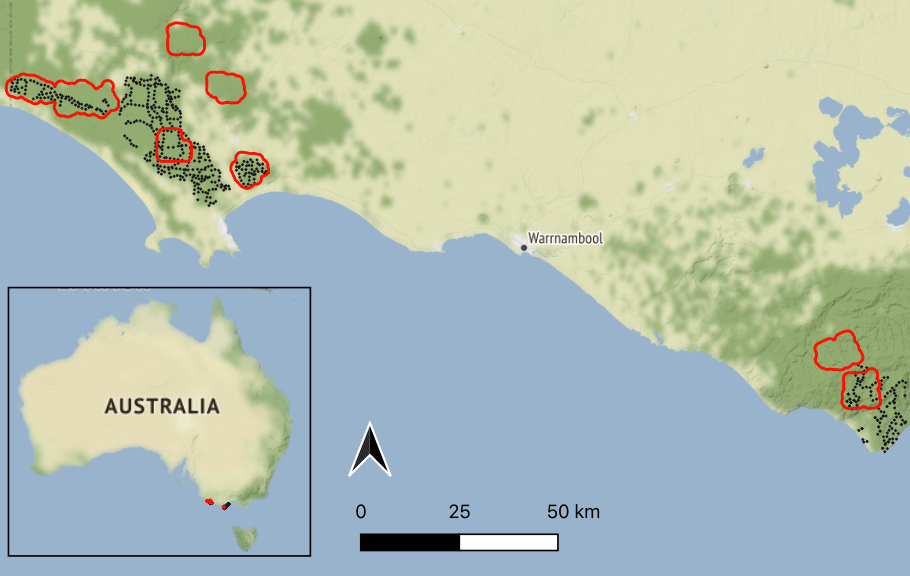
\includegraphics[width=1\linewidth]{figure/map_density} 

}

\caption{Locations of our eight study landscapes in south-west Victoria, Australia (red outlines). Note the two Lower Glenelg National Park landscapes in the far west are shown as one but are separated by a river. Locations of fox poison-bait stations are denoted by black dots. The Glenelg region is to the west and Otway region to the east. Native vegetation is indicated by dark green, with hill shading. \textit{Map tiles by Stamen Design, under CC BY 3.0, map data by OpenStreetMap, under CC BY SA.}}\label{fig:density-map}
\end{figure}
\newpage

\hypertarget{results-2}{%
\section{Results}\label{results-2}}

\hypertarget{fox-occurrence}{%
\subsection{Fox occurrence}\label{fox-occurrence}}

In the Glenelg region, there was a clear difference in fox occurrence between paired impact (poison-baited) and non-impact landscapes for replicates 1 and 3, but only a marginal difference for replicate 2 (Fig. \ref{fig:foxplot}). In the Otway region, fox occurrence increased by 22\% in the non-impact landscape, and decreased by 43\% in the impact landscape over the three years (occurrence probability averaged at each camera-trap in the landscape). Fox occurrence in the Otway region was generally lower than the Glenelg region, with less fine-scale spatial variation. For example, fox occurrence was predicted to be spatially consistent across the entire Otway region in 2018 (Fig. \ref{fig:foxplot}). Fox model summaries and spatial standard error estimates are presented in Appendix C section \ref{density-app-fox}.

\hypertarget{feral-cats-in-the-glenelg-region}{%
\subsection{Feral cats in the Glenelg region}\label{feral-cats-in-the-glenelg-region}}

Across the six landscapes in the Glenelg region, we recorded 251 cat detections from 32,232 camera-trap nights (Table \ref{tab:density-stats}). We were able to identify 64\% of cat detections to the individual level; a total of 67 cats (6 -- 13 individuals per landscape). The exponential detector function was supported over the half-normal function (Table \ref{tab:density-aic-g-1}). The null model was more strongly supported than models with vegetation impacts on cat density and/or linear time trends on \emph{g}\textsubscript{0} (Table \ref{tab:density-aic-g-2}).

At a fine spatial scale, the model with a linear relationship between fox occurrence and cat density was strongly supported (AIC\textsubscript{c} 2.76 better than the null; Table \ref{tab:density-aic-g-3}). It indicated that cat density declined as fox occurrence increased (-0.32; 95\% CI: -0.57 - -0.07; Fig. \ref{fig:dcor}). There was no evidence of an impact of fox occurrence on cat detectability (Table \ref{tab:density-aic-g-3}). Regression splines added additional model parameters without changing predictions (Fig. \ref{fig:dcor}), and so, all nonlinear models ranked below their linear counterparts (Table \ref{tab:density-aic-g-3}).

Our hypothesis that cat density would be higher in landscapes with fox control was supported for the first and third replicate pairs: estimated cat densities were 2.5 (95\% CI: 1.5 - 4.2) and 3.7 (95\% CI: 1.4 - 9.5) times higher in the impact landscape than the paired non-impact landscape, respectively (Fig. \ref{fig:diffg}). For the second landscape pair, however, the estimated difference was positive but negligible (1.1; 95\% CI: 0.69 - 1.69). At the landscape level, there was some evidence that cat detectability was affected by fox occurrence; however the AIC\textsubscript{c} score was only 0.95 units better than the constant detectability model (Table \ref{tab:density-aic-g-4}) and the estimated effects were weak with high uncertainty. The detectability of cats in their activity centre (\emph{g}\textsubscript{0}) tended to increase with the probability of fox occurrence (0.24; 95\% CI: -0.32 - 0.80), as did sigma (0.13; 95\% CI: -0.14 - 0.41).

\hypertarget{feral-cats-in-the-otway-region}{%
\subsection{Feral cats in the Otway region}\label{feral-cats-in-the-otway-region}}

In the Otway region, we recorded 970 cat detections from 36,272 camera-trap nights (Table \ref{tab:density-stats}). We were able to identify 53\% of cat detections to the individual level; a total of 93 cats (20 -- 30 individuals per landscape). The exponential detector function was strongly supported over the half-normal function (Table \ref{tab:density-aic-o-1}). The null model was more strongly supported than the models with vegetation impacts on cat density and/or linear time trends on \emph{g}\textsubscript{0} (Table \ref{tab:density-aic-o-2}).

There was some evidence that cat density was negatively correlated with fox occurrence at a fine spatial scale: the two top-ranked models included a linear and a non-linear effect of fox occurrence on cat density, respectively; however, a model without a fox occurrence term received similar support (dAIC\textsubscript{c} = 0.80; Table \ref{tab:density-aic-o-3}). The 95\% confidence interval around the linear coefficient from the top-ranked model marginally overlapped zero (-0.26; 95\% CI: -0.55 - 0.02) indicating that cat density declined as fox occurrence increased in the Otways at a similar rate to Glenelg, but with slightly greater uncertainty (Fig. \ref{fig:dcor}). However, the equivalent nonlinear model predicted that cat density only declined (at a steeper rate) in the mid-high range of fox occurrence probability (Fig. \ref{fig:dcor}). Equivalent pairs of linear model and nonlinear models were indistinguishable based on AIC\textsubscript{c} scores (Table \ref{tab:density-aic-o-3}).
There was also strong support for an effect of fox occurrence on cat detectability at a fine spatial scale (Fig. \ref{fig:detcor}; Table \ref{tab:density-aic-o-4}). Where fox occurrence was higher, cats were less detectable in their activity centres (i.e., negative association with \emph{g}\textsubscript{0}; -0.69; 95\% CI: -1.11 - -0.27; Fig. \ref{fig:detcor}A) and ranged further (i.e., positive association with sigma; coefficient 0.30; 95\% CI: 0.13 - 0.47; Fig. \ref{fig:detcor}B). The equivalent nonlinear model predicted detectability changes to have occurred only in the low-mid range of fox occurrence (Fig. \ref{fig:detcor}).

Our hypothesis that cat density in the impact landscape would increase relative to the non-impact landscape with fox control was supported, however there was considerable uncertainty. Cat density tended to be lower in the impact than non-impact landscape prior to fox-baiting (i.e., in 2017), although the confidence intervals for the two density estimates overlapped substantially (Fig. \ref{fig:diffo}). In 2018, cat density decreased in the non-impact landscape and increased in the impact landscape, converging to near-identical density estimates. These patterns continued into 2019, with cat density now somewhat higher in the impact landscape than non-impact landscape. Overlap in the response ratio confidence intervals for successive years was high, but the comparison between 2017 to 2019 suggests a meaningful increase in cat density at the impact landscape relative to the non-impact landscape (Fig. \ref{fig:diffo}B). Like the fine scale model, there was strong evidence that cat detectability was impacted by fox occurrence (Table \ref{tab:density-aic-o-4}).

\newpage

\(~\)

\(~\)

\(~\)
\begin{figure}

{\centering 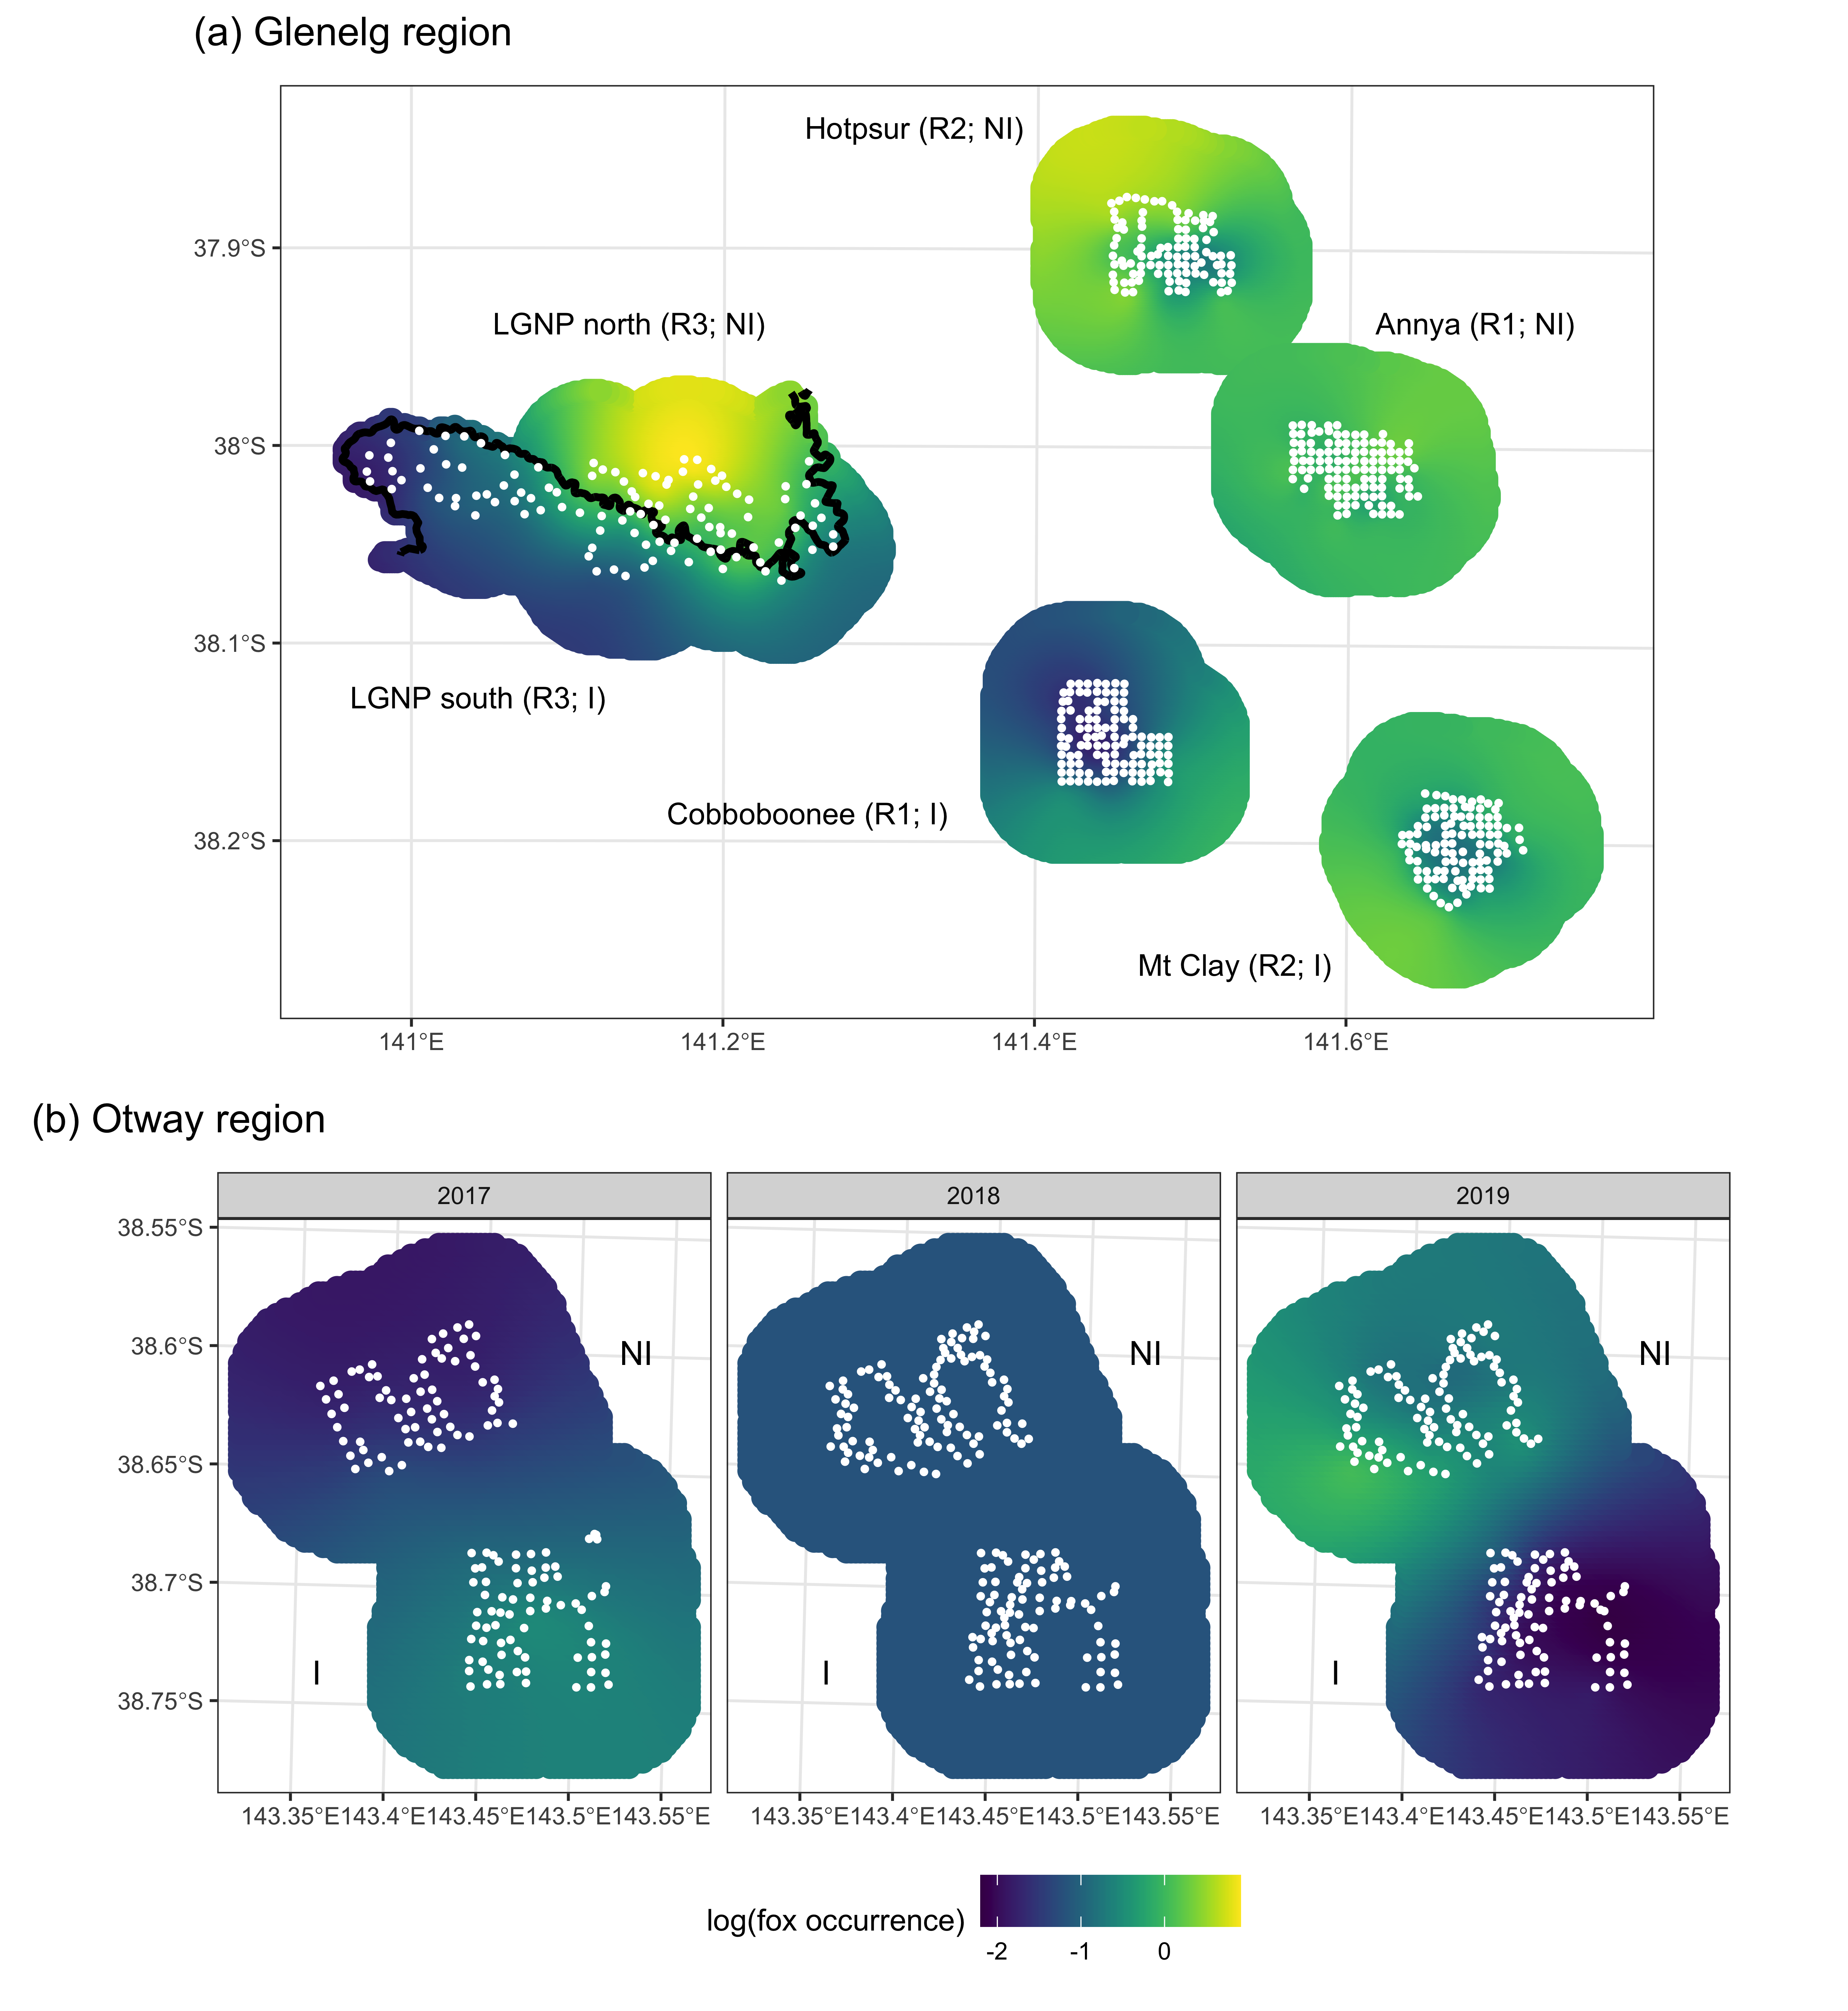
\includegraphics[width=1\linewidth]{figure/fox_occ_map} 

}

\caption{Predicted red fox \textit{Vulpes vulpes} occurrence derived from generalised additive models within each impact (I) and paired non-impact (NI) landscape in the Glenelg (a) and Otway (b) regions, Australia. White dots represent camera-trap sites. Predicted fox occurrence was used as a predictor of feral cat Felis catus density in the spatial mark-resight models.}\label{fig:foxplot}
\end{figure}
\newpage

\(~\)

\(~\)

\(~\)
\begin{figure}

{\centering 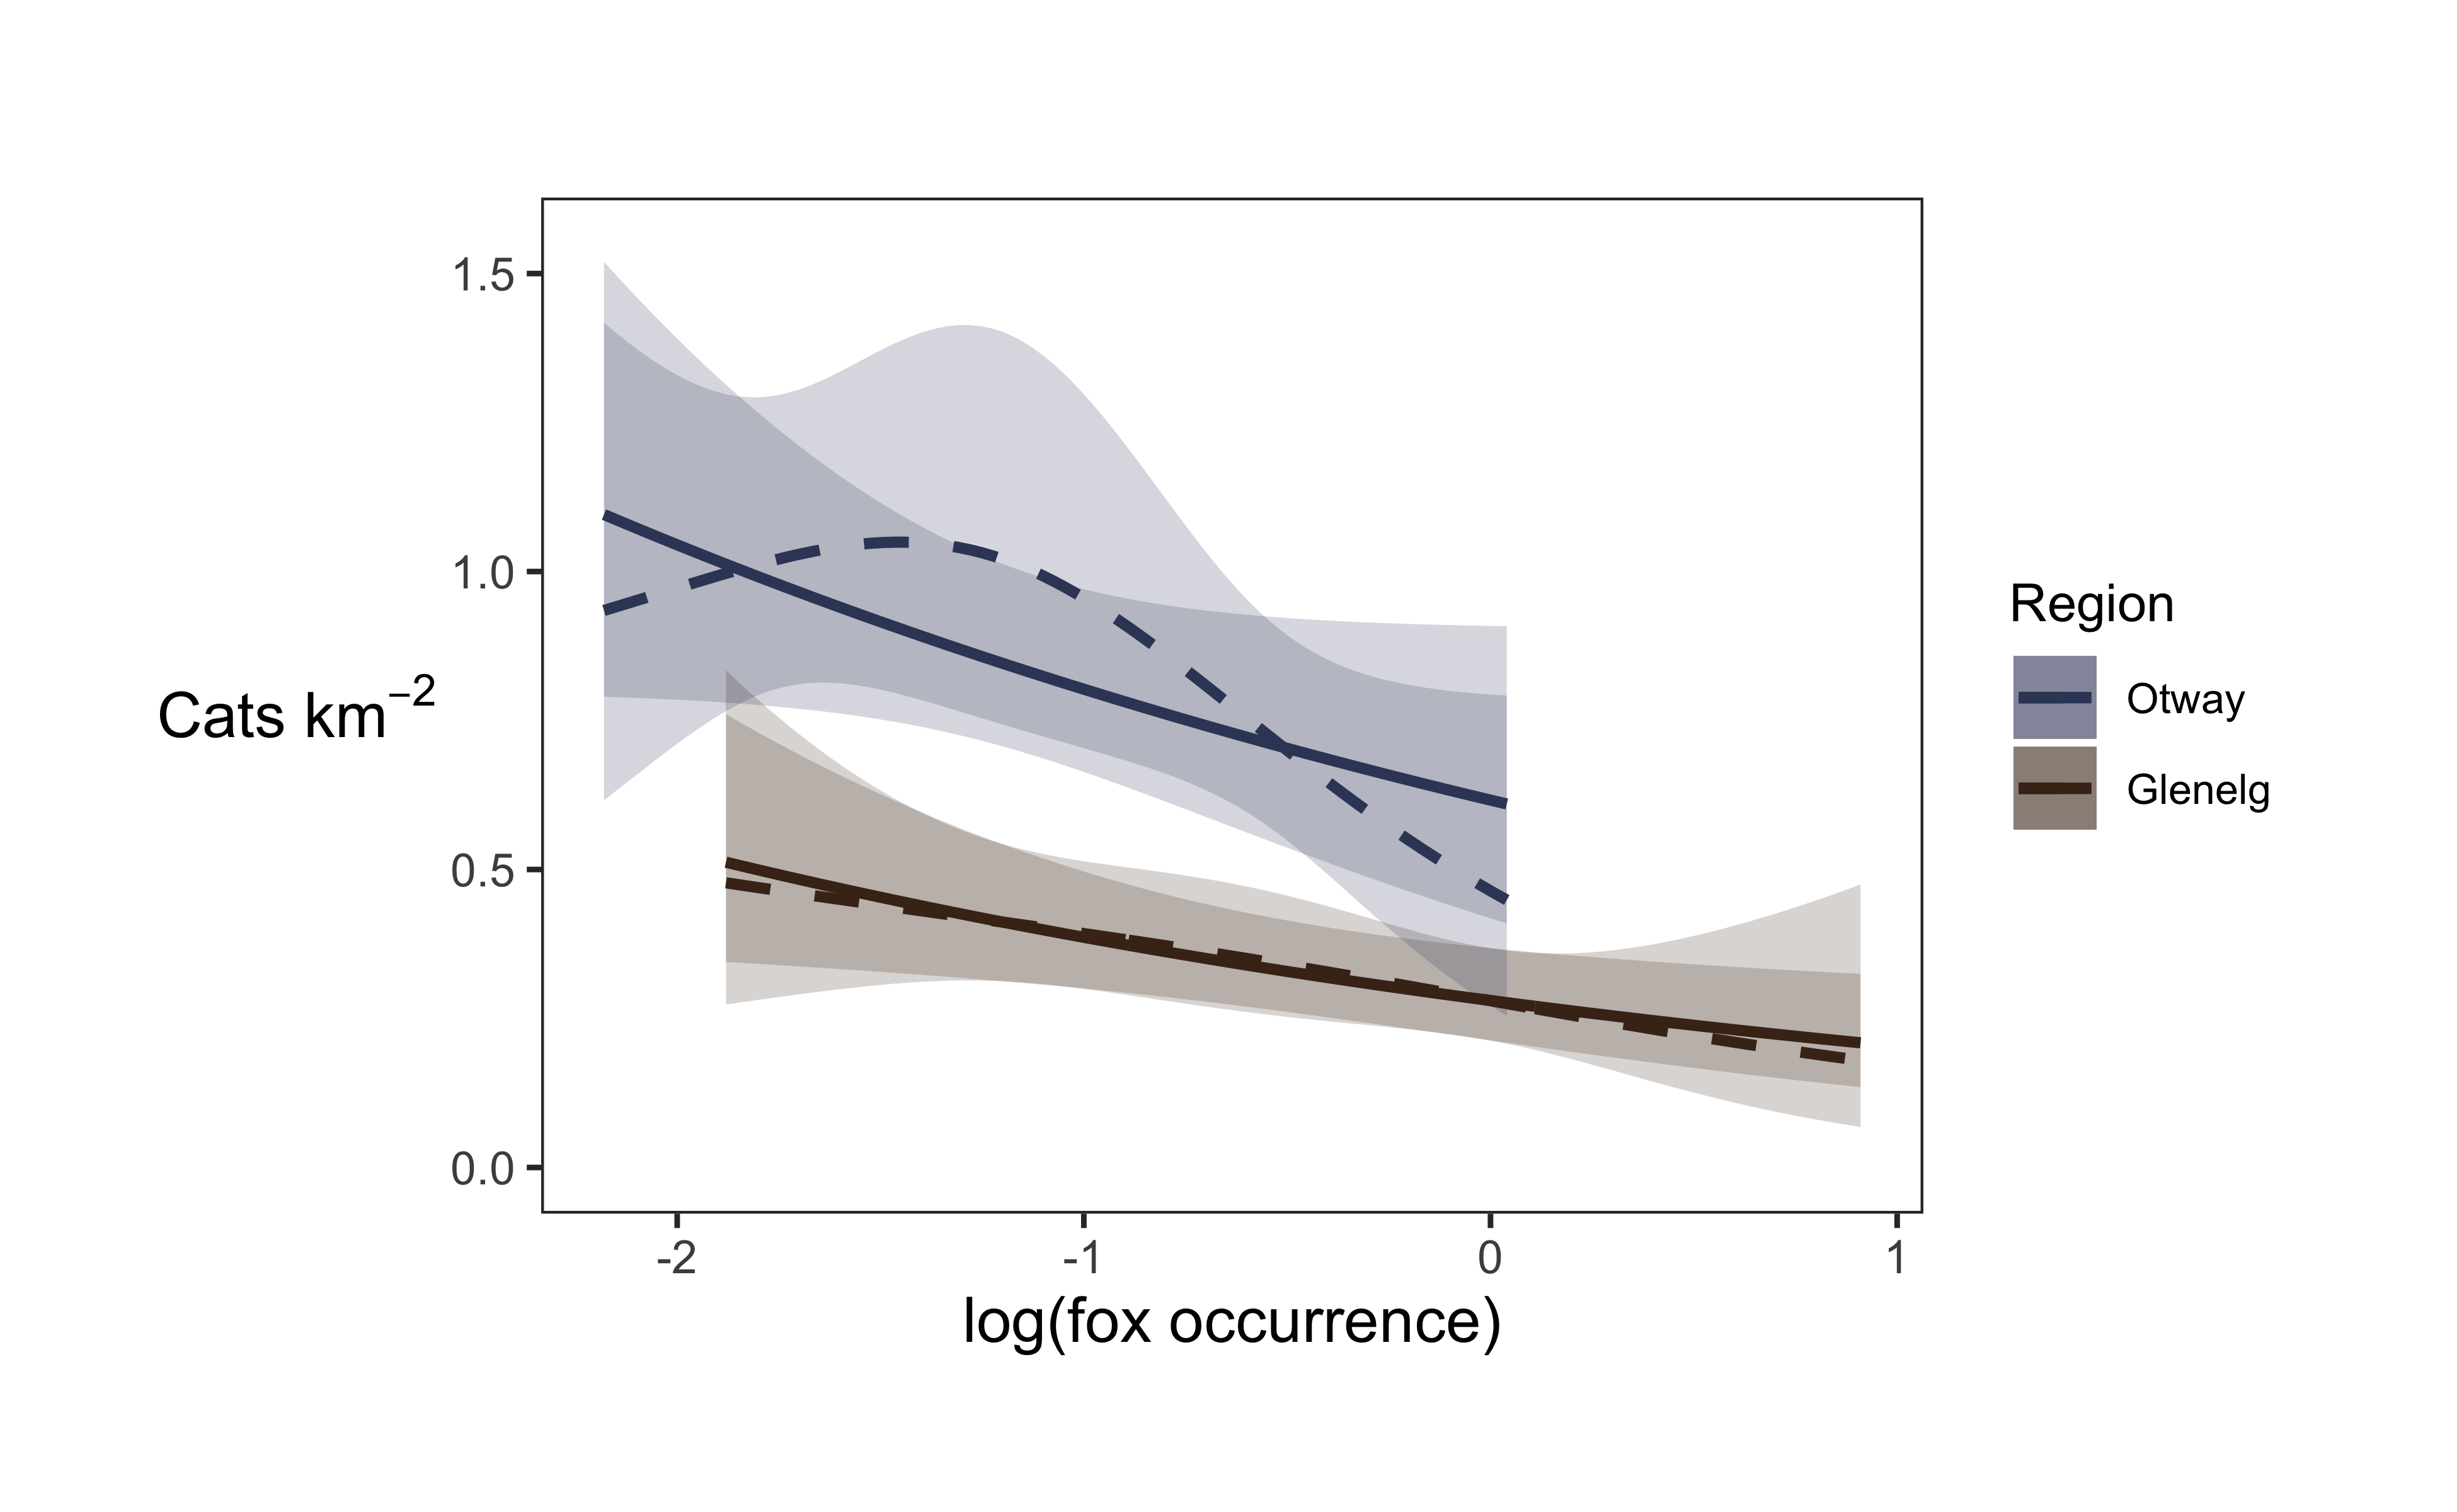
\includegraphics[width=1\linewidth]{figure/foxD_600dpi} 

}

\caption{Linear (solid lines) and nonlinear (dashed lines) models predicted that feral cat \textit{Felis catus} density increased with declining probability of red fox \textit{Vulpes vulpes} occurrence (log-transformed) in the Glenelg and Otway regions, Australia. Shaded areas indicate 95\% confidence intervals.}\label{fig:dcor}
\end{figure}
\newpage

\(~\)

\(~\)

\(~\)
\begin{figure}

{\centering 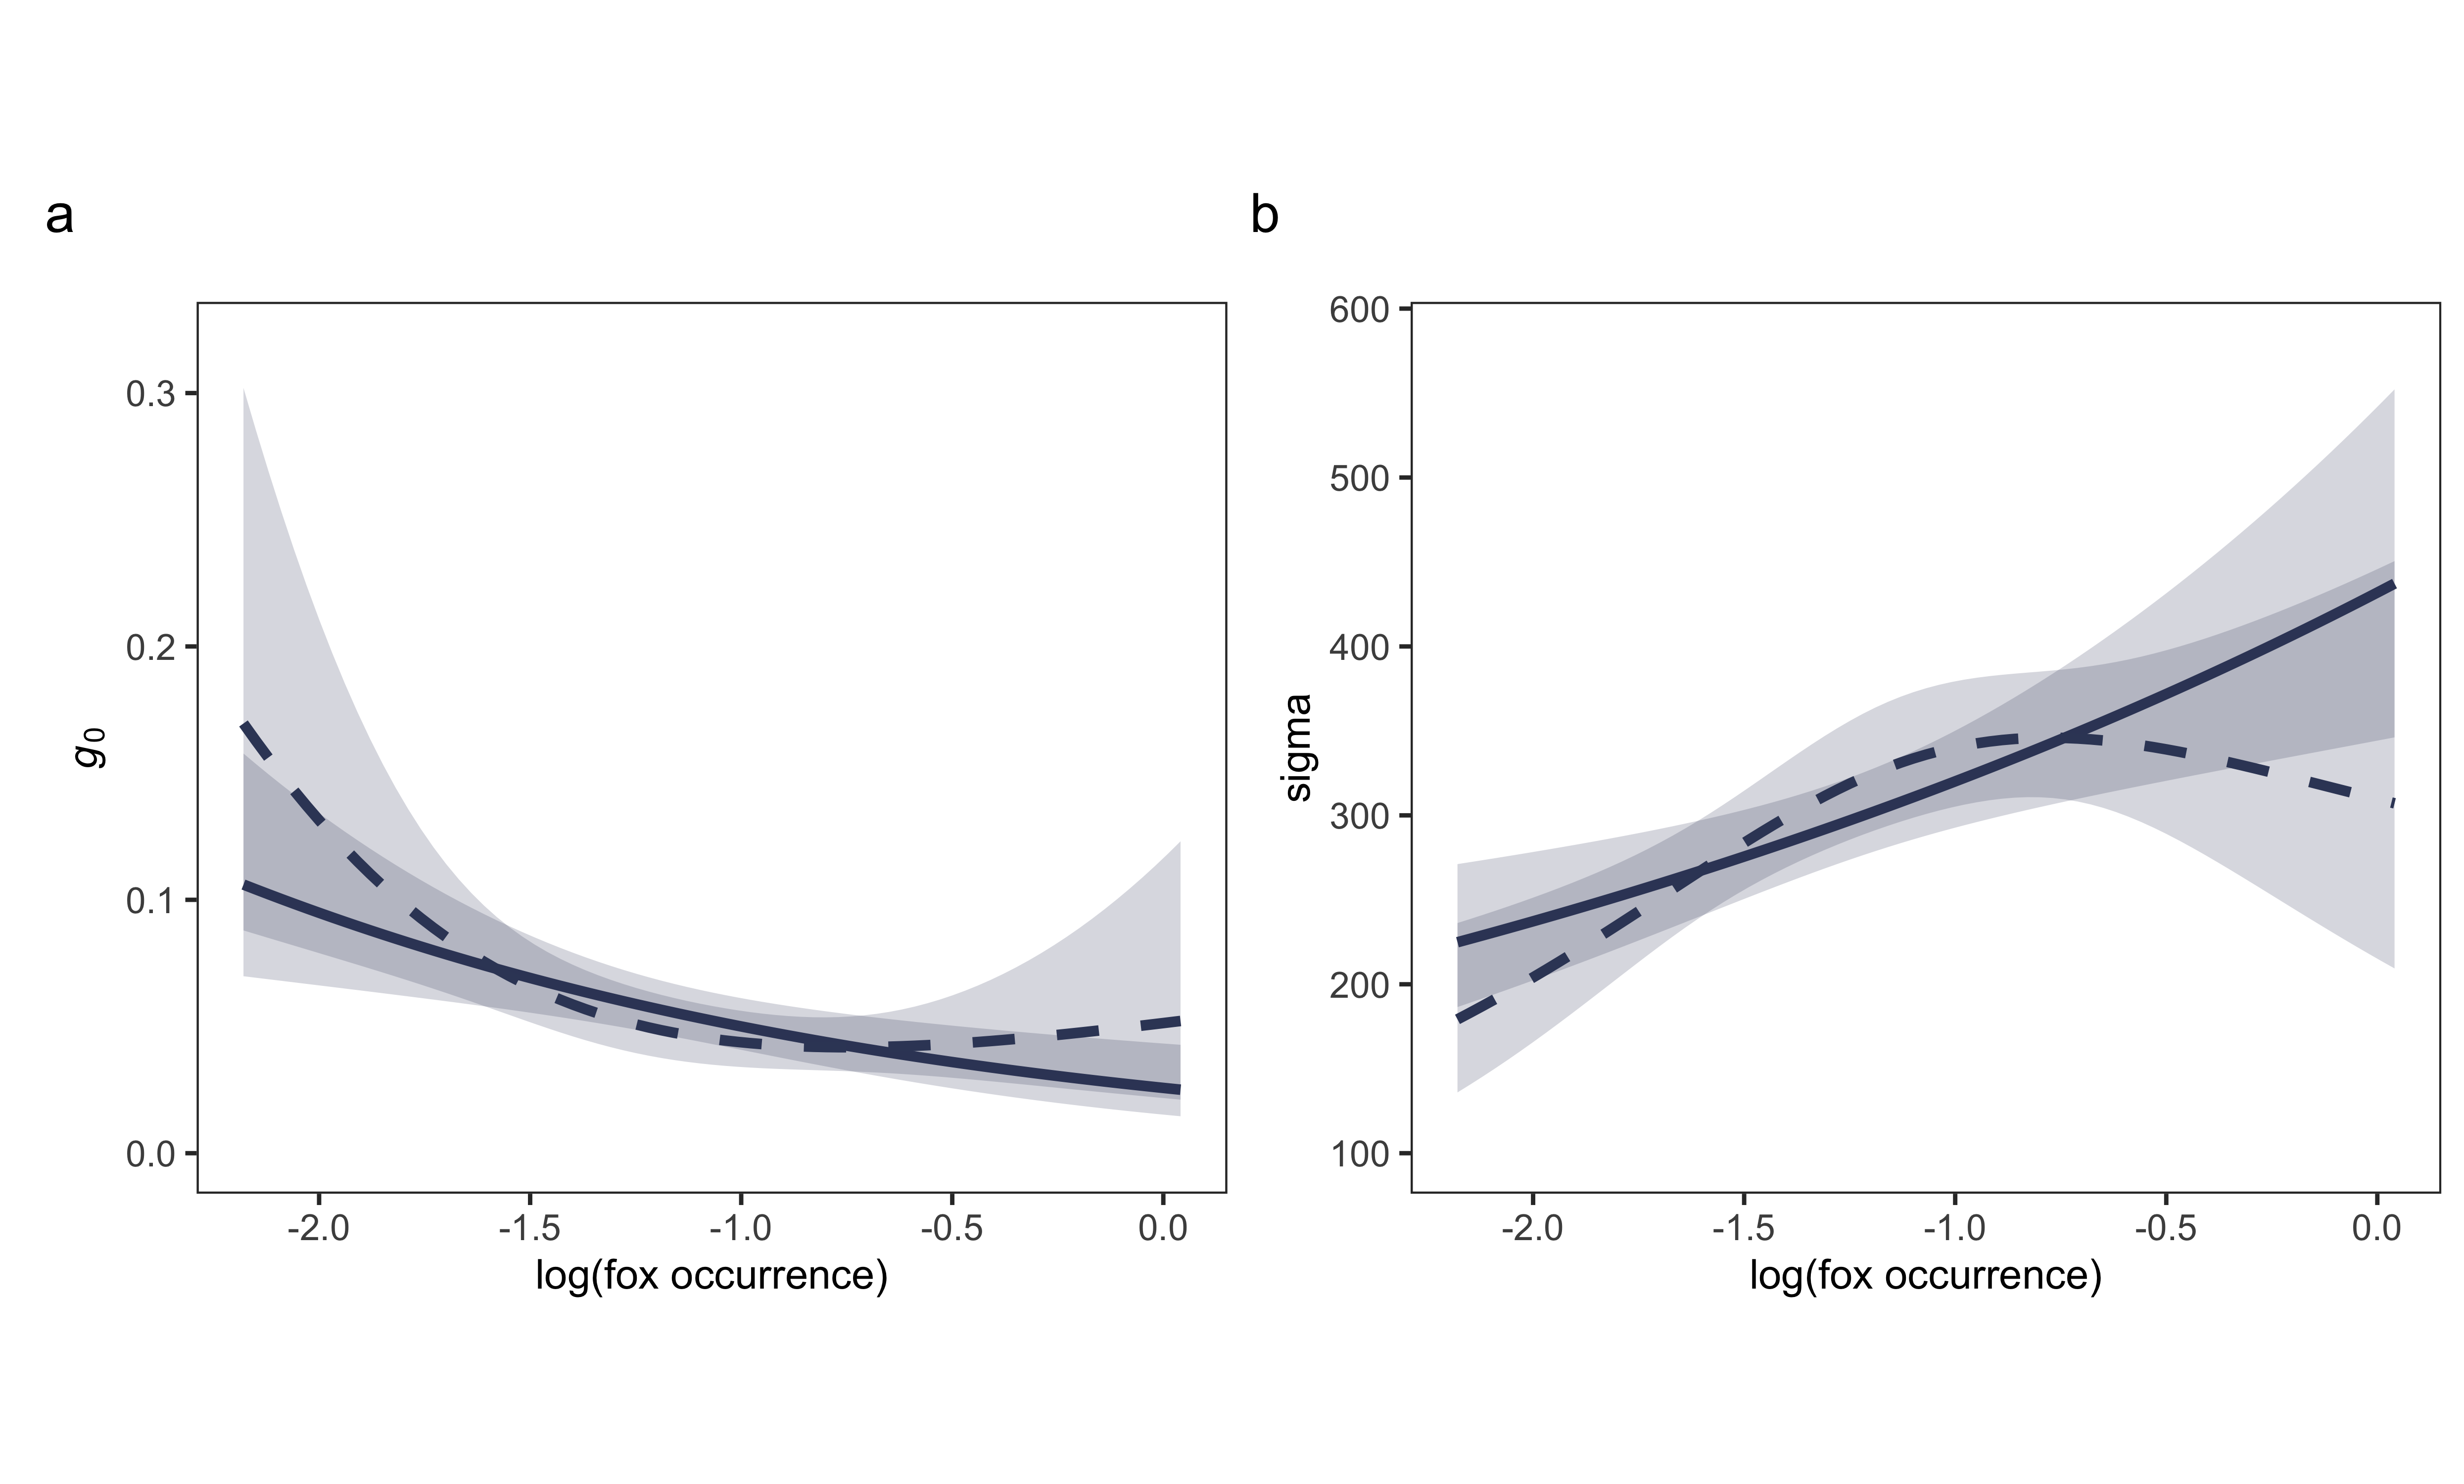
\includegraphics[width=1\linewidth]{figure/foxDet_otways_600dpi} 

}

\caption{Linear (solid lines) and nonlinear (dashed lines) models of feral cat \textit{Felis catus} detectability as a function of log-transformed red fox \textit{Vulpes vulpes} occurrence in the Otway Ranges, Australia. The probability of detecting a feral cat in its activity centre per 24-hour occasion (\textit{g}\textsubscript{0}) decreased with the probability of fox occurrence (a), while sigma (which is related to home range size; exponential detection function) increased (b). Shaded areas indicate 95\% confidence intervals.}\label{fig:detcor}
\end{figure}
\newpage

\(~\)

\(~\)

\(~\)
\begin{figure}

{\centering 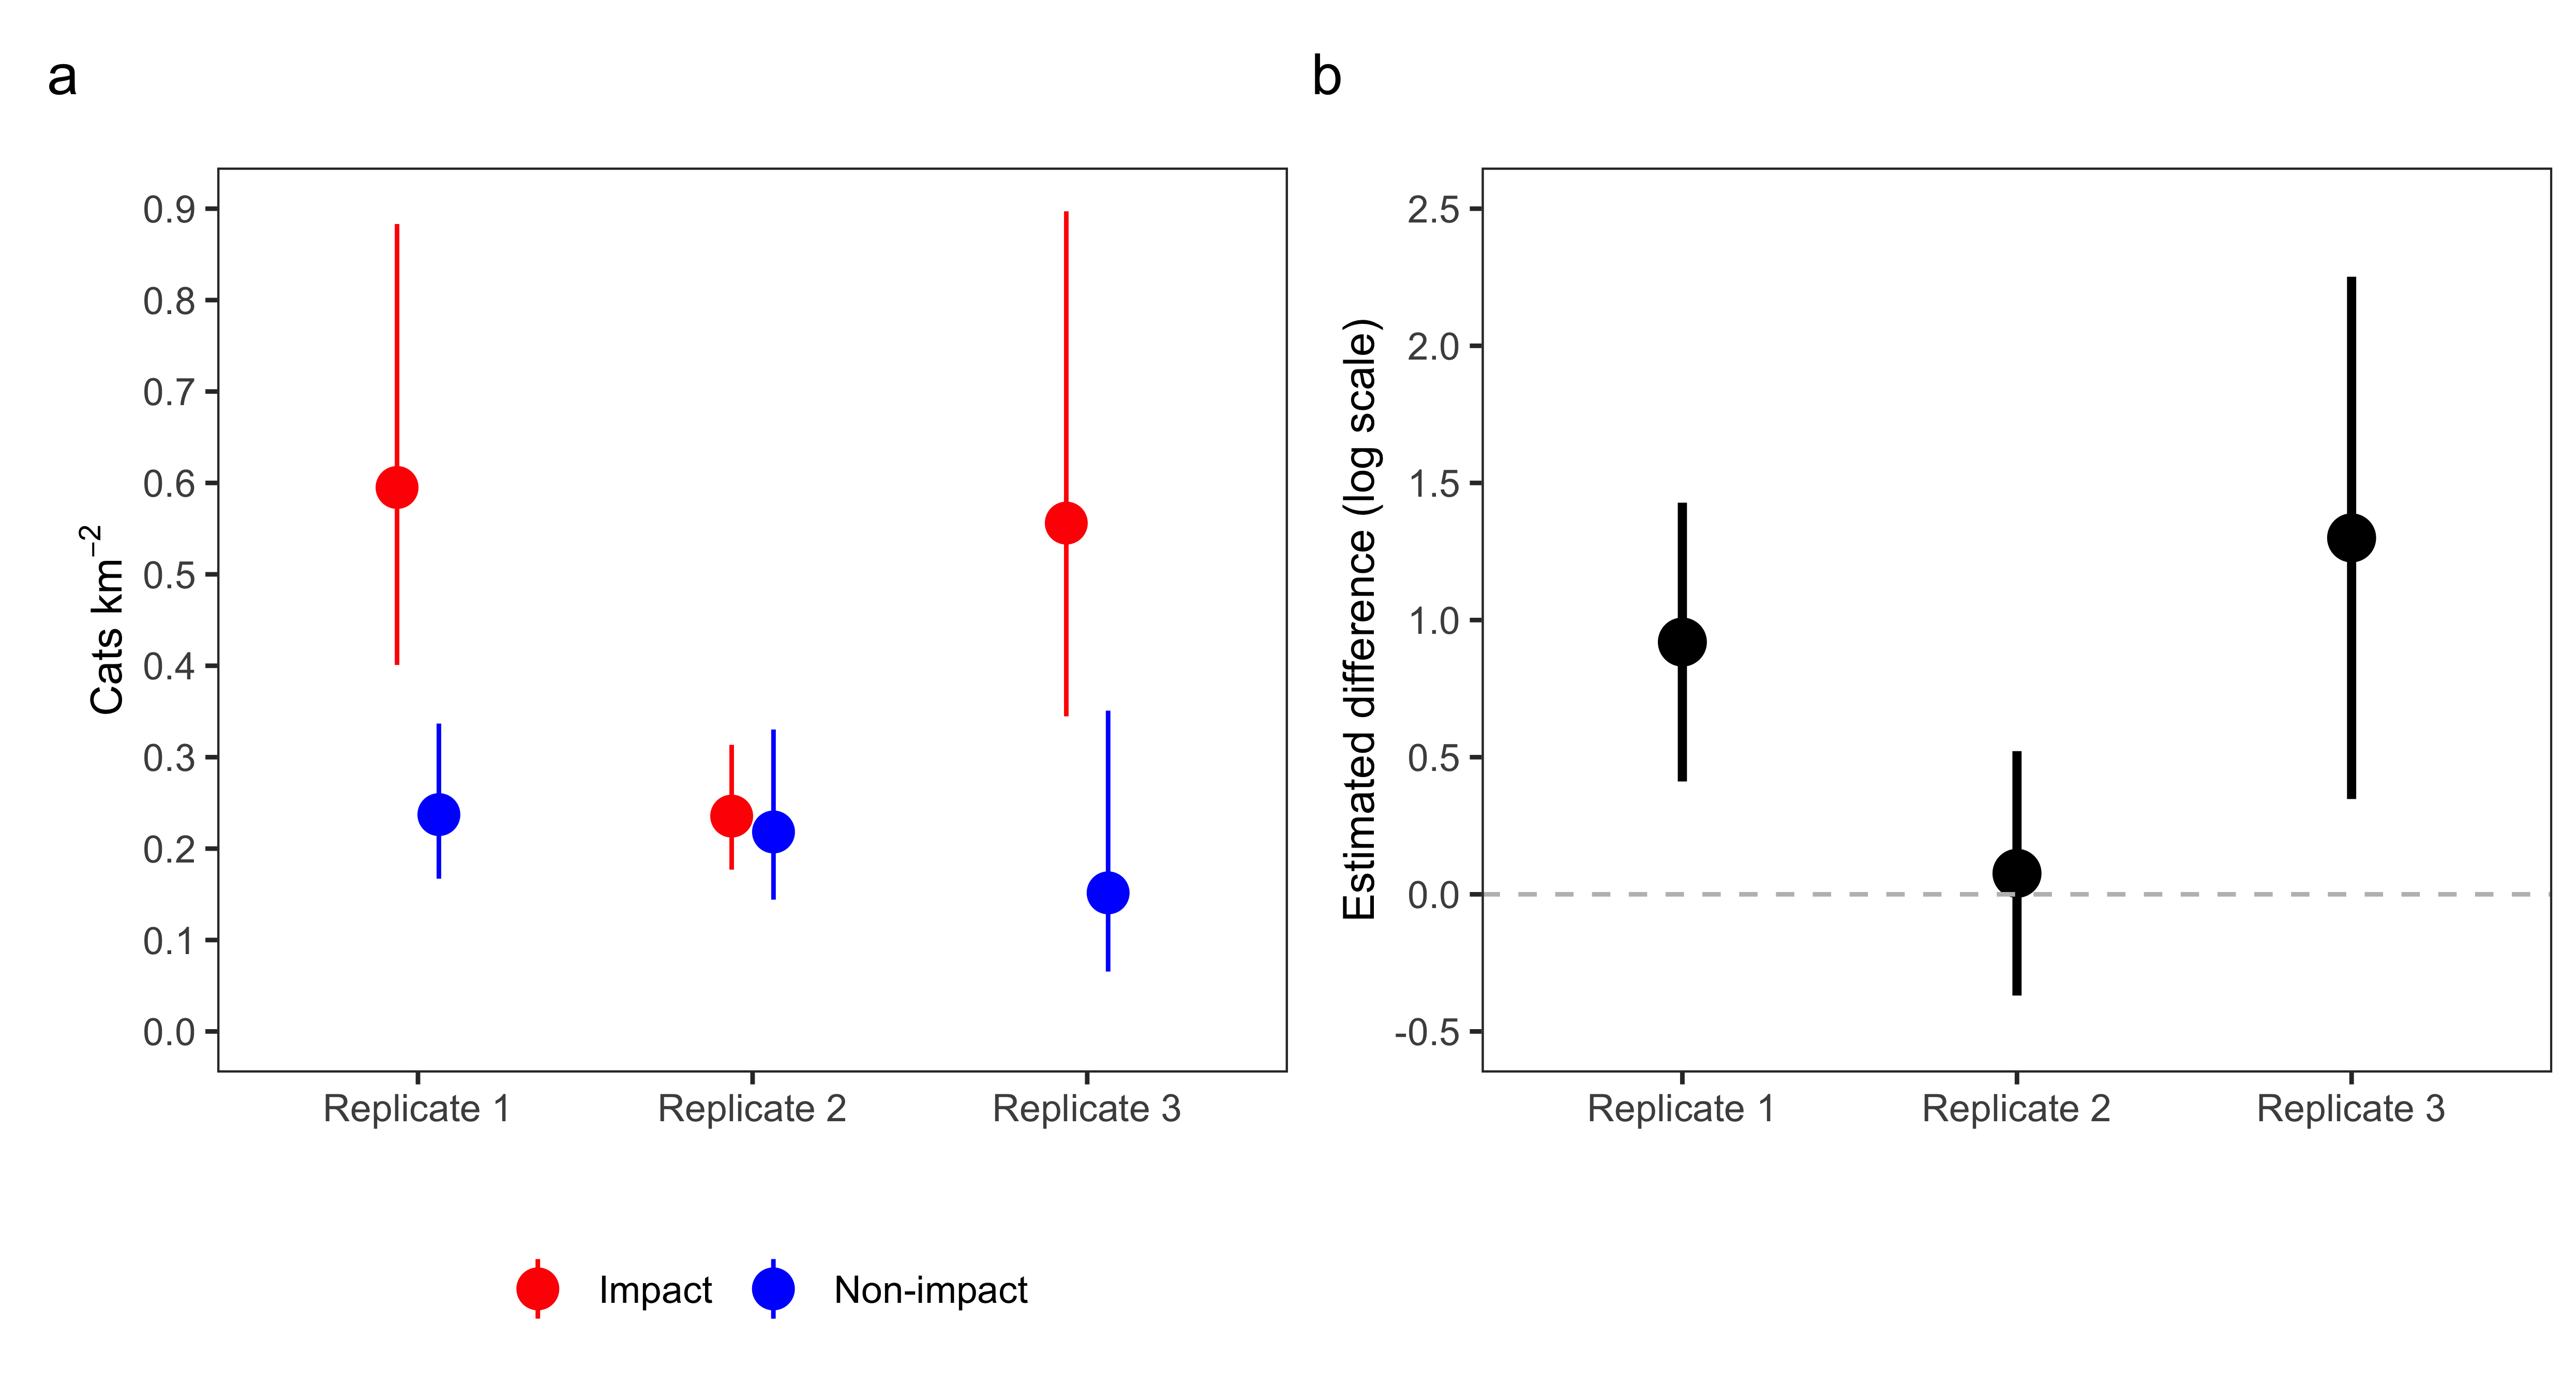
\includegraphics[width=1\linewidth]{figure/glenelg_estimates_600dpi} 

}

\caption{Landscape-scale feral cat \textit{Felis catus} density estimates (a) and response ratio of cat density in the impact landscape relative to the paired non-impact landscape for each replicate (b) in the Glenelg region, Australia. Poison-baiting for foxes \textit{Vulpes vulpes} has been conducted in the impact landscapes for more than 13 years. Grey dashed line represents no difference between the paired landscapes. Error bars represent 95\% confidence intervals.}\label{fig:diffg}
\end{figure}
\newpage

\(~\)

\(~\)

\(~\)
\begin{figure}

{\centering 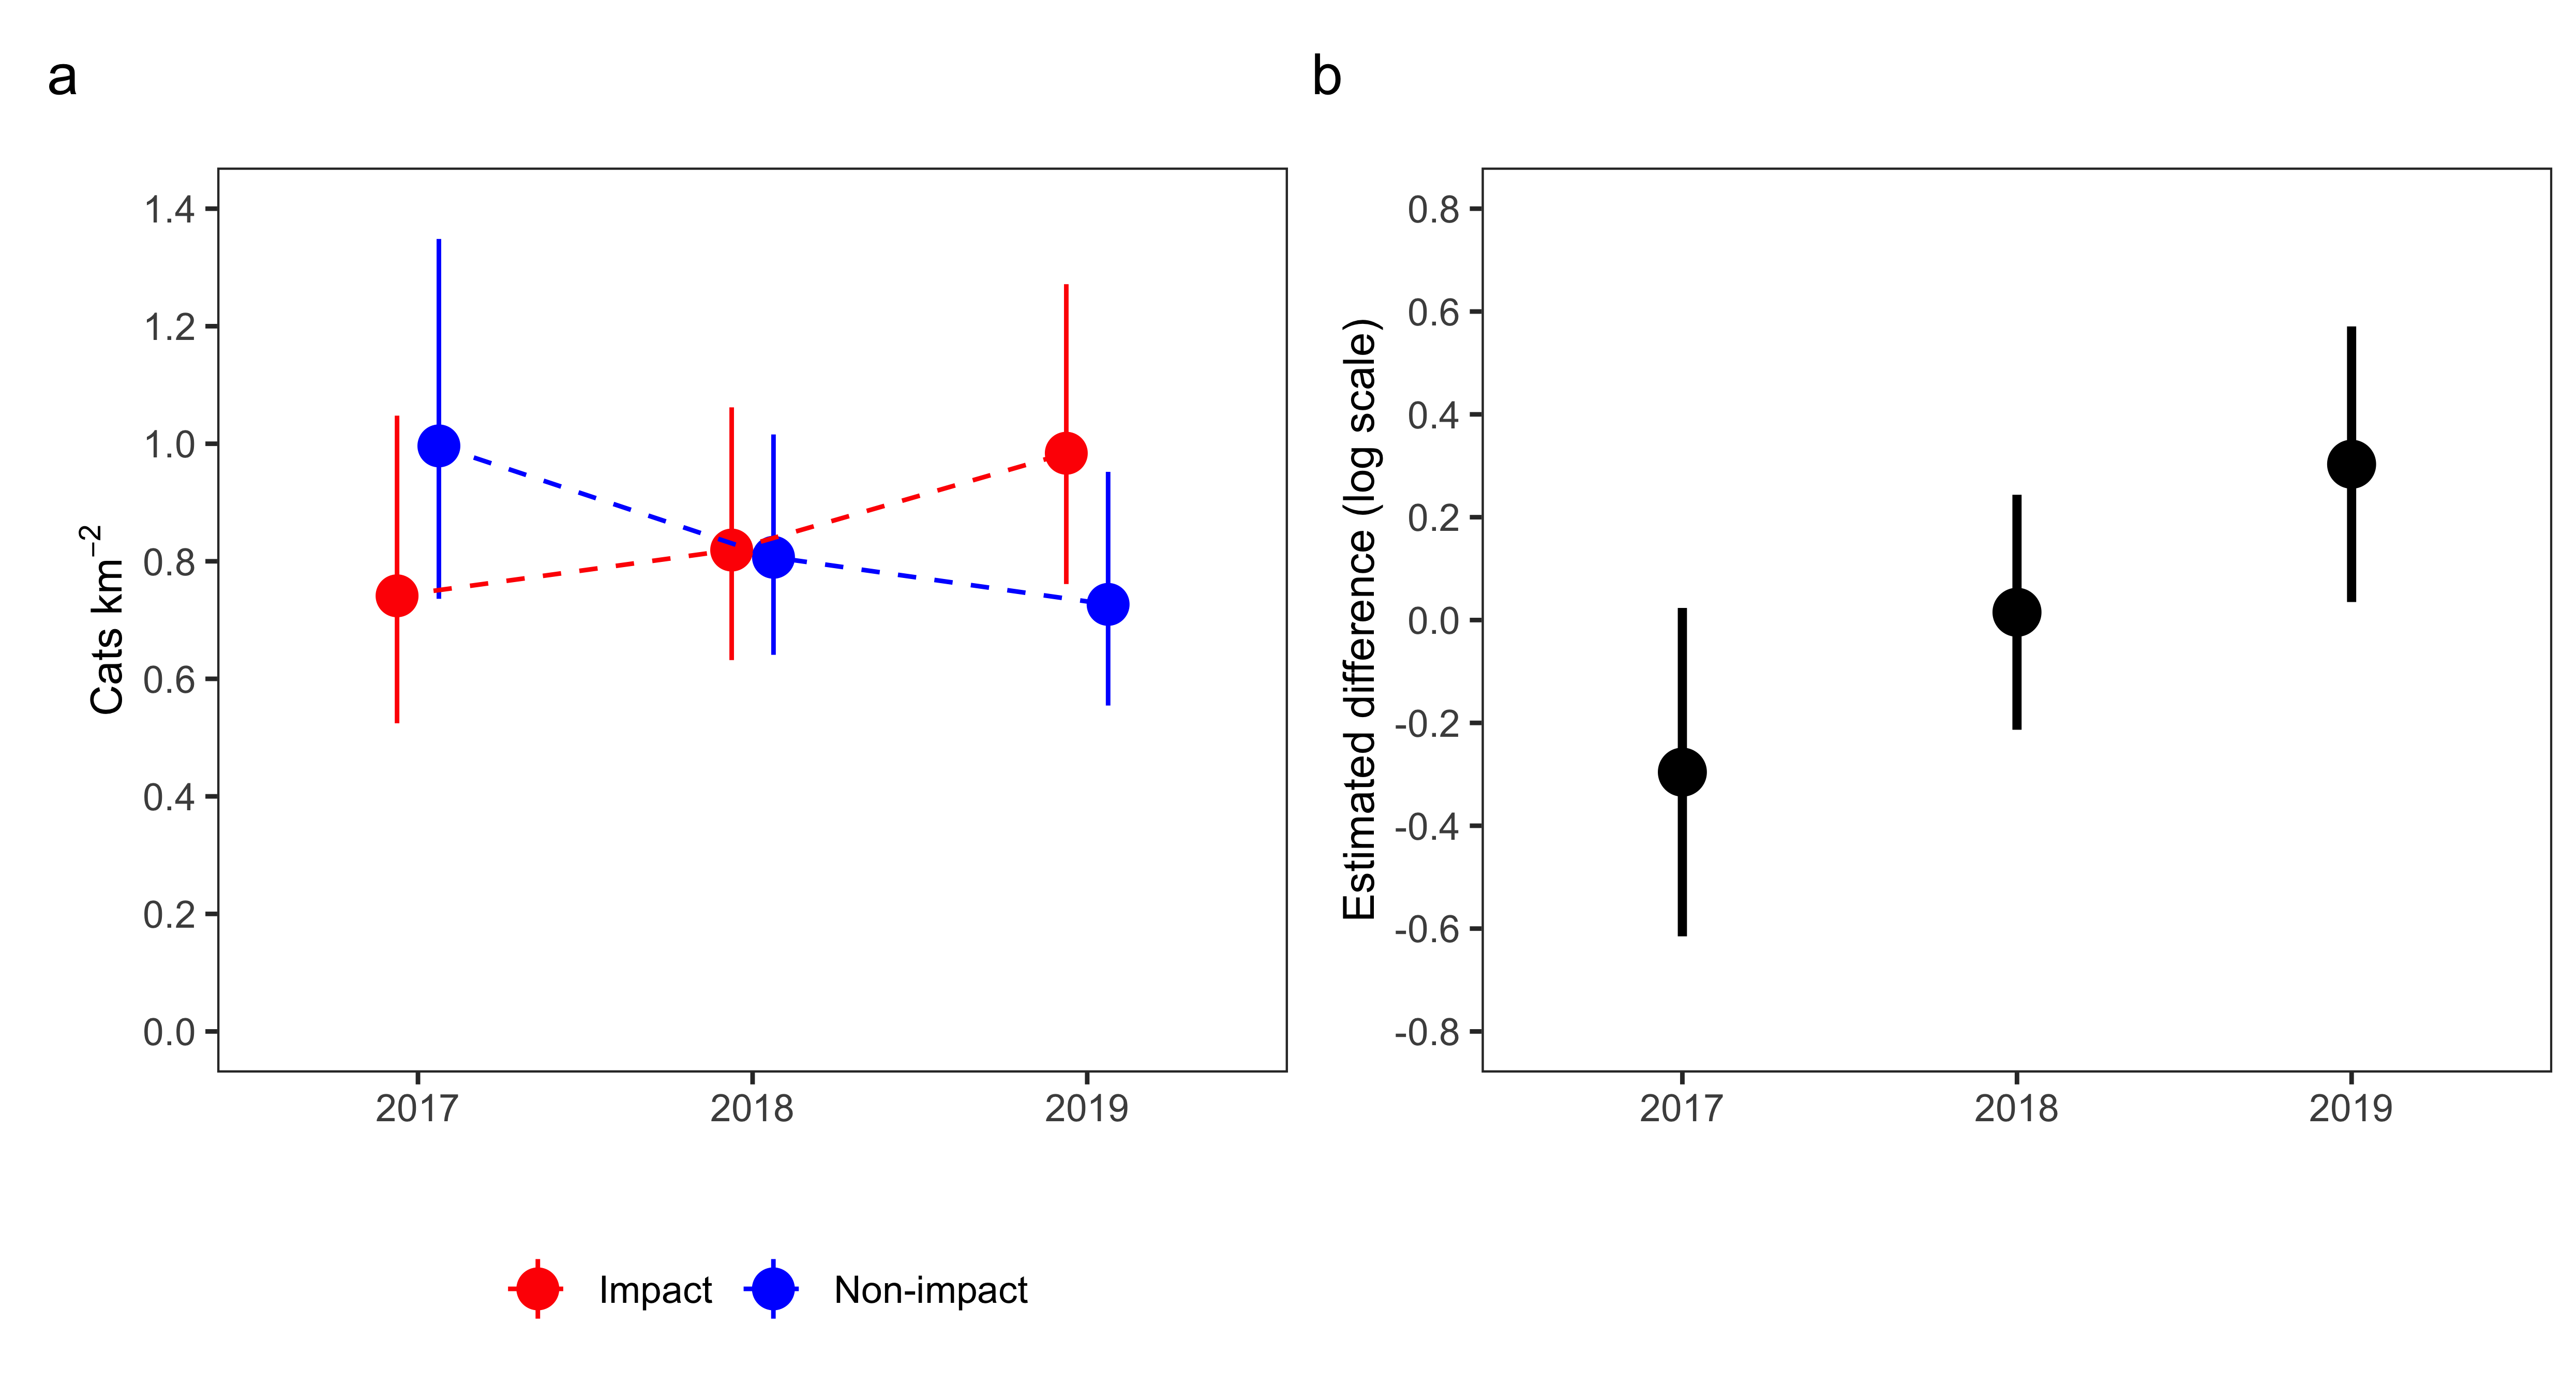
\includegraphics[width=1\linewidth]{figure/otways_estimates_600dpi} 

}

\caption{Landscape-scale feral cat \textit{Felis catus} density estimates (a) and response ratio of cat density in the impact landscape relative to the non-impact landscape for each survey year (b) in the Otway region, Australia. In 2017, surveys were conducted approximately two months before lethal red fox \textit{Vulpes vulpes} control commenced in the impact landscape; control lapsed for six months prior to the 2018 survey. Error bars represent 95\% confidence intervals. Overlap with the grey dashed line in (b) represents no difference in density between the paired landscapes for that year; the proportion overlap between response ratio confidence intervals across years provides evidence for a change in difference.}\label{fig:diffo}
\end{figure}
\newpage

\hypertarget{discussion-2}{%
\section{Discussion}\label{discussion-2}}

Our study is one of the first to provide replicated, experimental evidence that apex predator suppression can increase mesopredator population density. Our study provides two lines of evidence that foxes can exert top-down control on feral cats in the forests of south-eastern Australia: feral cat density was (1) higher where fine-scale fox occurrence probability was lowest, and (2) commonly higher in landscapes where fox control occurred. This is alarming because targeted fox control is a widely used conservation strategy; this unintended consequence could dampen benefits to native prey and even further threaten these species. However, as our findings highlight, mesopredator release of cats following fox control is unlikely to occur universally; the degree of fox suppression varies and fox-cat interactions are likely to be context and scale-dependent. More broadly, our study illustrates how correlative and experimental approaches provide complementary lines of evidence when investigating interactions between predator species, and the importance of disentangling changes in population density from changes in detectability.

We were able to exploit a gradient in fox occurrence caused by lethal control to investigate associations between cat density and fox occurrence at a fine spatial scale across two separate regions. At this scale, we observed a consistently negative association between cat density and fox occurrence, supporting our first hypothesis, although there was more uncertainty around the relationship in the Otway region. We acknowledge that it could also simply reflect differences in niche preference, rather than foxes excluding cats or cats avoiding foxes. However, we consider this unlikely given we observed the relationship across an artificial gradient of fox occurrence caused by lethal control.

There is contention around whether linear regression is appropriate for investigating correlations between different predator species, as subordinate predators may only be suppressed when apex predator abundance is high (Johnson \& VanDerWal 2009). We found no evidence of non-linear associations between foxes and cats in the Glenelg region, while linear and non-linear models performed equally well in the Otway region. Non-linear models in the Otway region predicted that cat density declined only in the mid-high range of fox occurrence, while behavioural changes were seen in the low-mid range of fox occurrence. Perhaps cats can successfully avoid foxes through behavioural change where foxes are rare, but this is ineffective where foxes are common. This could explain the lack of evidence for foxes impacting cat detectability in the Glenelg region where fox occupancy is relatively high. Alternatively, behavioural changes may be untenable for cats in the Glenelg region because small mammal abundance is relatively low and fox avoidance strategies likely come at the expense of hunting success (Sih 1980; Wilson \emph{et al.} 2010).

Where fox occurrence was higher in the Otway Ranges, cats were less detectable in their activity centres and ranged further (Fig. \ref{fig:detcor}). Low detectability is likely to correlate with fewer apex predator encounters, and has been observed in other predator interaction studies (e.g.~Lombardi \emph{et al.} 2017). An increase in cat ranging behaviour (sigma) with fox control supports observations made by Molsher \emph{et al.} (2017), and may reflect a direct avoidance strategy. Animal movement rates are expected to increase in response to unpredictable threats (Riotte-Lambert \& Matthiopoulos 2020). Alternatively, cats may consider foxes predictable and avoid locations they frequent, thus having to range further to obtain the same amount of food resources. In a similar forest habitat, Buckmaster (2012) observed large `holes' in the home range of each GPS-collared cat; they confirmed that this was not due to an absence of prey and hypothesised that it could be due to apex predator avoidance. Regardless of the cause, variation in mesopredator detectability and movement rates with apex predator populations has serious implications for the interpretation of studies that compare relative abundance indices and spatial overlap of predator species without disentangling behaviour and detectability from density (Efford \& Dawson 2012; Neilson \emph{et al.} 2018; Stewart \emph{et al.} 2018; Broadley \emph{et al.} 2019).

In the Glenelg region where fox-baiting had occurred for more than 13 years, feral cat density was considerably higher in two out of three distinct landscapes than in similar, unbaited landscapes. The outlier is most likely due to limited suppression of foxes at Mt Clay despite ongoing fox control (Fig. \ref{fig:foxplot}). Mt Clay is a small forest block surrounded entirely by unbaited farmland. Simulation modelling indicates that the size of the baited area is a key driver of the degree of reduction in the fox population (Hradsky \emph{et al.} 2019; Francis \emph{et al.} 2020). Studies of fox-cat (and other predator-predator) interactions often use the presence of a management program as a proxy for lower apex predator abundance and distribution (e.g.~Hunter \emph{et al.} 2018). Our findings strongly indicate the need to directly measure the apex predator population in order to reliably interpret the responses of subordinate species (Salo \emph{et al.} 2010).

In the Otway region, we observed a weaker--but increasing--effect of fox control on cat density, to be expected from a recently commenced and less intensive fox-baiting program. The short duration of baiting in the Otway region may mean that changes in adult cat density are yet to fully manifest as foxes potentially suppress cats by reducing recruitment rates. Cats may also respond to an increase in shared prey availability following fox suppression (Stobo-Wilson \emph{et al.} 2020a). A time-lagged release of cats following fox control would explain eruptions and subsequent crashes commonly observed in shared mammalian prey populations two to ten years following fox control commencement (Duncan \emph{et al.} 2020). Alternatively, top-down suppression by foxes and competition may be weaker in this highly productive environment where prey abundance was relatively high, fox occurrence was already relatively low, and overall cat densities were consistently high (Johnson \& VanDerWal 2009; Greenville \emph{et al.} 2014; Newsome \emph{et al.} 2017). Our surveys provide important baselines against which to compare future changes in predator populations as the fox-baiting program continues.

Our study is among the very few which have used a direct measure of density to test mesopredator release. Previous studies have mostly used live capture-rates to infer population density, without accounting for behavioural or detectability changes (e.g.~Arjo \emph{et al.} 2007; Karki \emph{et al.} 2007; Thompson \& Gese 2007; Berger \emph{et al.} 2008; Jones \emph{et al.} 2008). Contention about mesopredator release has centred on such methods (Hayward \emph{et al.} 2015); as well as unaccounted species interactions in complex predator guilds (Levi \& Wilmers 2012; Jachowski \emph{et al.} 2020). In contrast, our study tests the mesopredator release theory using a combined behavioural and numerical approach, in a system with a simplified carnivore guild. One limitation of our approach is that uncertainty from our fox occurrence models was not propagated into the spatial mark-resight models. A full Bayesian integration of the fox occurrence analysis and the spatial mark-resight model to address this is not yet implemented. The development of open population spatial mark-resight models would also improve parameter estimates for multi-season surveys.

The results of our study may explain why pest management that only targets foxes--one of the most prevalent conservation actions in Australia--does not consistently improve native prey persistence (Dexter \& Murray 2009; Robley \emph{et al.} 2014; Wayne \emph{et al.} 2017a; Lindenmayer \emph{et al.} 2018; Duncan \emph{et al.} 2020). More evidence is required to understand the circumstances in which lethal fox control increases cat density, particularly the role of baseline fox and prey densities. A more integrated approach to invasive predator management, where foxes and cats are simultaneously or otherwise optimally controlled could substantially improve biodiversity outcomes (Risbey \emph{et al.} 2000; Comer \emph{et al.} 2020). If this is not feasible, changes in invasive mesopredator density and the outcomes for native prey species should be closely monitored as part of any control program for invasive apex predators, with triggers for ceasing apex predator control or commencing integrated management if single-species control proves counterproductive for the conservation of threatened prey species.

\hypertarget{diel}{%
\chapter{Spatial variation in predator diel activity patterns -- feral cats avoid red foxes in time, not space}\label{diel}}

\hypertarget{abstract-3}{%
\section*{Abstract}\label{abstract-3}}
\addcontentsline{toc}{section}{Abstract}

Understanding the constraints that apex predators impose on subordinate species is important for anticipating the outcomes of predator management. Subordinate predators may avoid dominant predators in time or space, making it difficult to quantify changes in antipredator behaviours unless joint spatiotemporal analyses are used.

In this study, we tested whether an invasive apex predator (red fox \emph{Vulpes vulpes}) suppresses or alters the spatiotemporal activity of an invasive mesopredator (feral cat \emph{Felis catus}). We surveyed these predators using 3667 camera-trap deployments across two regions of south-eastern Australia; foxes were poison-baited in some landscapes within each region. The simplified predator guild in these regions allowed sharp focus on the interactions between these species across experimental gradients of fox (apex predator) activity. We used generalised additive models to quantify predator overall activity across space and fluctuations in activity throughout the daily cycle (i.e., diel activity patterns).

When averaged across the study region, red foxes and feral cats had very similar diel activity patterns; however, there was important differentiation at a finer scale. Feral cats did not reduce their overall activity when fox counts at the camera-trap were high but shifted diel activity patterns to less risky times of the day. In dry habitats of both regions, cats shifted from being nocturnal-crepuscular to mostly diurnal. In wet forests, diel activity patterns were absent for foxes; cats became more nocturnal - avoiding dawn in particular - when fox counts were high. These changes in diel activity patterns may facilitate spatial coexistence between these two invasive predators, potentially shifting impacts onto different native prey species.

It is well-appreciated that overall predator activity varies spatially and fluctuates throughout the daily cycle, however, our study demonstrates that diel activity patterns also vary across space, likely mediated by both landscape context and fear. Apex predator avoidance appears to be dynamic across landscapes of fear--- this key nuance is overlooked when simply comparing the average activity overlap between two species or the spatial overlap of species occurrence in isolation.

\newpage

\hypertarget{introduction-3}{%
\section{Introduction}\label{introduction-3}}

Predators shape ecosystems through both predation and the fear of predation (Creel \& Christianson 2008; Ritchie \& Johnson 2009). Fear-induced behavioural suppression could be as detrimental to populations of subordinate species than predation itself (Schmitz \emph{et al.} 2004; Preisser \emph{et al.} 2005). These non-consumptive apex predator effects are expected to be strong drivers of mesopredator behaviour, particularly when resource competition is high (Ritchie \& Johnson 2009). Strengthening or relaxing antipredator behaviours can have cascading effects across the entire ecosystem: altering population demographics, species interactions, ecological function and human-wildlife coexistence (Brown \emph{et al.} 1999; Ripple \& Beschta 2004; Estes \emph{et al.} 2011; Gaynor \emph{et al.} 2019; Lamb \emph{et al.} 2020). Understanding how top predators constrain the behaviour of subordinate species is important in accurately predicting the ecosystem-wide consequences of predator management, such as reintroductions and lethal control (Gaynor \emph{et al.} 2021).

Spatial and/or temporal niche partitioning may allow predators to coexist by reducing both encounter-rates and resource overlap (Kronfeld-Schor \& Dayan 2003). However, avoidance behaviours may not be constantly employed by subordinate predators because perceived predation risk is temporally and spatially variable, and antipredator behaviours are traded-off against resource acquisition - limiting or relegating activity to suboptimal places or times (Lima \& Dill 1990; Lima \& Bednekoff 1999). And so, optimal predator avoidance strategies are also likely to vary across heterogeneous landscapes where resource availability (e.g., shelter, food) and perceived predation risks differ (Kauffman \emph{et al.} 2007; Willems \& Hill 2009; Wirsing \emph{et al.} 2021). For example, temporal predator avoidance may be preferable over spatial avoidance if food is constantly available throughout the day, and vice versa. These concepts are unified under the `ecology of fear' (Brown \emph{et al.} 1999) concept, which has gained increasing attention in recent times. Notably, the mesopredator release hypothesis has recently been expanded from increases in mesopredator abundance (Soulé \emph{et al.} 1988) to also include changes in mesopredator behaviour (Brashares \emph{et al.} 2010), following apex predator decline.

To accurately quantify avoidance within a predator guild, we first need to understand how the overall activity and diel activity patterns of each species varies `naturally' across landscapes, particularly for species with broad distributions. We generally consider how the overall activity of different predator species varies across their distributions, but often assume diel activity patterns to be constant across heterogeneous landscapes. In this paper, we use the term `overall activity' to refer to the number of `independent' predator detections (offset to account for different survey durations; analogous to activity and abundance indices), and `diel activity patterns' to refer to fluctuations in relative activity throughout the 24-hour daily cycle. Overall activity is a combined function of predator behaviour, population density and the detection process (disentangling these processes requires individual predator identification), whereas diel activity patterns are a behavioural trait (less likely to be affected by the detection process depending on survey methodology).

Despite modern predator survey technologies time-stamping detections, this information is commonly scrapped from analyses of predator avoidance, probably because joint modelling of overall activity and diel activity patterns is more complicated. When temporal avoidance is tested, it is usually considered in an ad-hoc fashion, by fitting separate models for spatial and temporal avoidance, or by repeating spatial analyses (e.g., resource selection functions) at different time periods (e.g., Smith \emph{et al.} 2019; Basille \emph{et al.} 2015; Kohl \emph{et al.} 2019). However, discretising the daily cycle into categorical periods (mostly day and night) introduces bias, assuming animals have complete step-changes in behaviour rather than progressive shifts across the daily cycle. Further, dawn and dusk are particularly important times for many predator species.

Generalised Additive Models (hereafter `GAMs') are increasingly being used to estimate animal diel activity patterns ( \emph{et al.} 2014) and offer a flexible framework to jointly consider overall activity. GAMs also have other benefits, including smoothing penalties to reduce overfitting, the ability to capture nonlinear interactions between multiple variables with different units and the ability to share information across categorical variables through hierarchical specifications (Wood 2017; Pedersen \emph{et al.} 2019). However, we are only aware of one study which allowed animal diel activity to interact with predation risk as a continuous variable (although without considering overall activity; Cunningham \emph{et al.} 2019).

The red fox \emph{Vulpes vulpes} (hereafter `fox'; \textasciitilde6 kg) and feral cat \emph{Felis catus} (hereafter `cat'; \textasciitilde4 kg) have devastating impacts on native prey throughout their introduced range, implicated in the extinction of \textasciitilde10 and 63 species, respectively (Doherty \emph{et al.} 2016). Cats are more difficult to manage, and so predator control programs often target only foxes (particularly through poison-baiting; Reddiex \emph{et al.} 2007). As foxes and cats compete for many of the same resources, there is concern that lethal fox control could cause a mesopredator (Soulé \emph{et al.} 1988) or competitor (Ruscoe \emph{et al.} 2011) release of feral cats (Glen \& Dickman 2005; Robley \emph{et al.} 2014; Marlow \emph{et al.} 2015a; Doherty \& Ritchie 2017; Wayne \emph{et al.} 2017a; Comer \emph{et al.} 2020). There is some evidence that feral cats increase in activity (although highly uncertain; Hunter \emph{et al.} 2018), density (Chapter \ref{density}) and alter their diets and use of space (Chapter \ref{density}; Molsher \emph{et al.} 2017) in response to fox control. Other studies have investigated potential spatial and temporal interactions between these invasive predators (e.g., Roshier \& Carter 2021), but not in response to fox control, or in a joint spatiotemporal framework that allows flexibility in cat avoidance behaviours in respect to differences in fox activity.

In this study, we explore how the overall activity and diel activity patterns of two competing invasive predators varies across heterogeneous landscapes, in response to (1) space and (2) vegetation types. We then investigated (3) whether cat diel activity patterns change in response to the overall level of fox activity. Our study was conducted in a simple predator system where foxes and cats are the only mammalian carnivores, and fox activity is manipulated using lethal control in some landscapes. This allowed sole focus on the interactions between these two predators, across an experimental gradient of apex predator (fox) activity. We illustrate how GAMs can provide a simple framework to jointly assess spatial and temporal animal activity patterns, as well as avoidance behaviours.

\newpage

\hypertarget{methods-3}{%
\section{Methods}\label{methods-3}}

\hypertarget{study-area-and-camera-trapping}{%
\subsection{Study area and camera-trapping}\label{study-area-and-camera-trapping}}

We compiled data from multiple smaller-scale camera-trap studies across two regions in south-west Victoria, Australia: the Glenelg region and Otway Ranges (Fig. \ref{fig:diel-map}). Introduced foxes and cats are the only medium-large functional mammalian terrestrial carnivores here: native dingoes \emph{Canis familiaris} are long-absent throughout, while tiger quolls \emph{Dasyurus maculatus} are long-absent in the Glenelg region and likely functionally extinct in the Otway Ranges (last confirmed sighting in 2014). In broad sections of each region, government land managers conduct ongoing targeted lethal fox control for biodiversity conservation. Poison-baits containing 3 mg of sodium mono-fluroacetate (`1080') are buried at a depth of 12 - 15 cm at 1-km intervals along accessible forest tracks and roads. Different road densities result in variable densities of poison-baits. Managers also frequently implement prescribed fire across both regions, primarily to reduce fuel loads to prevent large wildfires.

\hypertarget{glenelg-region-2}{%
\subsubsection{Glenelg region}\label{glenelg-region-2}}

In the Glenelg region, large patches of natural vegetation are fragmented by pastoral farming and residential properties (Fig. \ref{fig:diel-map}). Foxes in three distinct forest blocks in this region have been subject to poison-baiting since October 2005, with fortnightly bait replacements (Robley \emph{et al.} 2014). These forest blocks, along with three similar, unbaited forest blocks to the north are simultaneously surveyed annually under the `Glenelg Ark' fox control program since 2005, (40 camera-sites per block; Robley \emph{et al.} 2020). Hair-tubes were used to monitor small prey species from 2005 - 2013 (presented in Robley \emph{et al.} 2014), replaced by camera-traps from 2013 onwards (here we present camera-trap data from 2013 - 2019; Robley \emph{et al.} 2020). We also included a further 425 camera-trap deployments at unique locations from early 2018 (M.W.R., PhD surveys). This totals 2039 camera-trap deployments in the Glenelg region, collected in a control-impact experimental design (foxes had been continuously controlled for at 8 - 14 years in the treatment landscapes by the time of these surveys).

\hypertarget{otway-ranges-2}{%
\subsubsection{Otway Ranges}\label{otway-ranges-2}}

The Otway Ranges is a largely continuous patch of natural vegetation with a strong east-west rainfall gradient (Fig. \ref{fig:occ-map}). A matrix of cool temperate rainforest and wet forest at high-altitudes (up in the south-west descend into a large heathland directly north, and into dry forests and then heathlands to the north-east. Fox-baiting commenced in small sections of the Otway Ranges in 2008 and large-scale systematic baiting began in 2016 - 2017 under the `Otway Ark' program (Robley \emph{et al.} 2019). For the first six weeks, poison-baits were replaced weekly, then changing to ongoing monthly bait-replacement. There was a pause in baiting for approximately six months during the second half of 2018. Fox control recommenced in late 2018 with four weeks of fortnightly bait-replacement, before returning to monthly bait-replacement. A large section of the Otway Ranges to the north-west remains unbaited, but is monitored as an experimental non-treatment site (Robley \emph{et al.} 2019). Otway Ark managers survey 372 camera-trap sites annually (sequentially across the region); we present one `before' baiting survey and two `after' baiting surveys of each site from 2016 - 2018, totalling 1113 camera-trap deployments (Robley \emph{et al.} 2019). We also include data from an additional before-after control-impact surveys (one `before' baiting survey and two `after' bating surveys) in the western section of the Otway Ranges, conducted annually 2017 - 2019 (M.W.R PhD surveys). This added a further 195 sites and 524 camera-trap deployments.

\hypertarget{camera-trap-set-ups-1}{%
\subsubsection{Camera-trap set-ups}\label{camera-trap-set-ups-1}}

All camera-trap deployments consisted of a Reconyx (Holmen, Wisconsin) brand camera-trap (white or infrared flash), attached to a tree or a metal picket, facing a lure. The Glenelg Ark and Otway Ark fox monitoring programs positioned camera-traps at least 40 cm above ground on a tree or a metal picket and angled more strongly downwards toward a lure approximately 1 - 1.5 m away (Robley \emph{et al.} 2019, 2020). The lures consisted of peanut butter, golden syrup and rolled oats mixed into a small ball, placed within a tea strainer or PVC pipe container and secured either to the ground, or 20 - 60 cm above ground on a wooden stake. The M.W.R. PhD surveys across both regions positioned camera-traps lower on a tree (around 15 - 30 cm above the ground) angled only slightly downwards towards a tuna oil lure approximately 2 - 2.5 m away (detailed in Rees \emph{et al.} 2019). Camera-traps were active for an average of 47 days (maximum 93 days), totalling 172,052 trap-nights.

\hypertarget{data-preparation}{%
\subsection{Data preparation}\label{data-preparation}}

All data analysis was conducted in R version 3.6.3 (R Core Team 2020). We first used lorelograms to identify the minimum interval to approximate independence (Iannarilli \emph{et al.} 2019); this indicated discarding repeat detections of a species within 30 minutes was sufficient to reduce temporal autocorrelation. To account for day length variation across space and time, we extracted sunrise and sunset times for each camera-trap deployment using the `maptools' R-package (Bivand \& Lewin-Koh 2021) and adjusted detection times to be relative to sunrise and sunset using the average double anchoring approach described by Vazquez \emph{et al.} (2019). We then built a dataframe consisting of a row for each hour of the day (0 -- 23), for every camera-trap deployment (n = 3667), recording the total number of `independent' fox and feral cat detections within each hour across the camera-trap survey.

\hypertarget{generalised-additive-models-5}{%
\subsection{Generalised additive models}\label{generalised-additive-models-5}}

We modelled the total number of independent detections of each predator per hour for each camera-trap deployment (response variable) with generalised additive mixed-effect models implemented in the `mgcv' R-package (Wood 2017). We used the negative binomial family as overdispersion, but not zero-inflation, was detected with a poisson distribution using the `DHARMa' R-package (Hartig 2020). We specified the number of survey days as a model offset to account for differences in camera-trap survey duration, and a random intercept for each site to account for repeat sampling. For fox models, we also included a smooth effect of poison-bait density with separate responses per region to account for the effect of fox control (all figures in this manuscript are derived from fox models predicted to a no fox-baiting scenario). This formed the base model specification for each model we fitted; models differed in their specification of the cyclical hour smooth to provide inference on variations of predator diel activity across the four questions of interest; this is detailed in the sections below.

\hypertarget{how-does-predator-overall-activity-and-diel-activity-patterns-vary-across-space-model-1}{%
\subsubsection{How does predator overall activity and diel activity patterns vary across space? (model 1)}\label{how-does-predator-overall-activity-and-diel-activity-patterns-vary-across-space-model-1}}

To examine how the overall activity and diel activity patterns of each predator varied across space, we fit a model for each predator which included a tensor product interaction between a spatial smooth and hourly smooth. This allowed predators to have different activity levels across space (static across the years surveyed), as well as a variation in diel activity pattern across space. Space was modelled using camera-trap coordinates and a duchon spline basis (Miller \& Wood 2014). To examine how the relative strength of diel activity patterns changed across space, we plotted the percentage increase from the minimum to maximum activity estimate within the daily cycle for every predicted location (hereafter referred to as `diel activity pattern strength').

\hypertarget{how-does-predator-overall-activity-and-diel-activity-patterns-vary-across-vegetation-types-model-2}{%
\subsubsection{How does predator overall activity and diel activity patterns vary across vegetation types? (model 2)}\label{how-does-predator-overall-activity-and-diel-activity-patterns-vary-across-vegetation-types-model-2}}

Predator activity varied across space; we hypothesised that this was partly due to differences in vegetation type, based both on the observed spatial patterns and because vegetation type is a major driver of understorey habitat structure used as shelter and prey occurrence in these regions (Swan \emph{et al.} 2015; Hradsky \emph{et al.} 2017b). To test whether the diel activity pattern of each predator patterns varied among vegetation types, we identified the Ecological Vegetation Class group (hereafter ``vegetation type''; standard units for vegetation classification in Victoria; Department of Environment, Land, Water \& Planning 2020a) for each unique camera-trap site, totalling eight vegetation types. As rainforests are interspersed (primarily in low lying gullies) at fine-scales throughout wet and damp forests in the south-eastern Otway Ranges, we merged them together (hereafter referred to as `wet forests'). We then estimated predator activity across vegetation types using a hierarchical model specification: a global smoother for hour (i.e., average response) and group-level smoothers with shared wiggliness for the seven vegetation types (``model GS'' detailed in Pedersen \emph{et al.} 2019). We also included a random effect to account for differences in overall activity levels between the two regions.

\hypertarget{do-feral-cats-avoid-foxes-in-space-or-time-model-3}{%
\subsubsection{Do feral cats avoid foxes in space or time? (model 3)}\label{do-feral-cats-avoid-foxes-in-space-or-time-model-3}}

Fox diel activity across vegetation types showed strong similarity between all vegetation types except wet forests. To examine whether cats avoid foxes in space or time, we therefore modelled fox-induced changes in feral cat diel activity separately for wet forest and dry vegetation types. We further split dry vegetation types by region for replication. We refer to the resulting variable as `habitat type', which had three levels: (i) wet forests and rainforests in the western Otway Ranges (`wet\_otways'), (ii) dry EVC groups of the Otway Ranges (`dry\_otways') and (iii) the Glenelg region (`dry\_glenelg'). We hypothesised that cats would avoid foxes in time by becoming more diurnal in dry vegetation types where foxes were mostly nocturnal, but not in wet forests where fox activity had little variation across the daily cycle.

To investigate changes in feral cat diel activity across the range of observed fox activity, we calculated the total number of fox detections for each camera-trap deployment, adjusted by the survey duration by dividing by the log of the number of survey days (hereafter `adjusted fox counts'). We modelled an interaction between hour (cyclical spine) and adjusted fox counts (thin plate regression spline with shrinkage - meaning fox effects could be entirely removed from the model if not supported by sufficient data), allowing cats to have nonlinear responses to both hour and adjusted fox counts. We fit separate tensor product interactions for each habitat type (using a `by-variable' term). For a direct visual comparison to fox activity, we fit another fox model where a diel curve was estimated separately across each of the three habitat types.

\newpage
\begin{figure}

{\centering 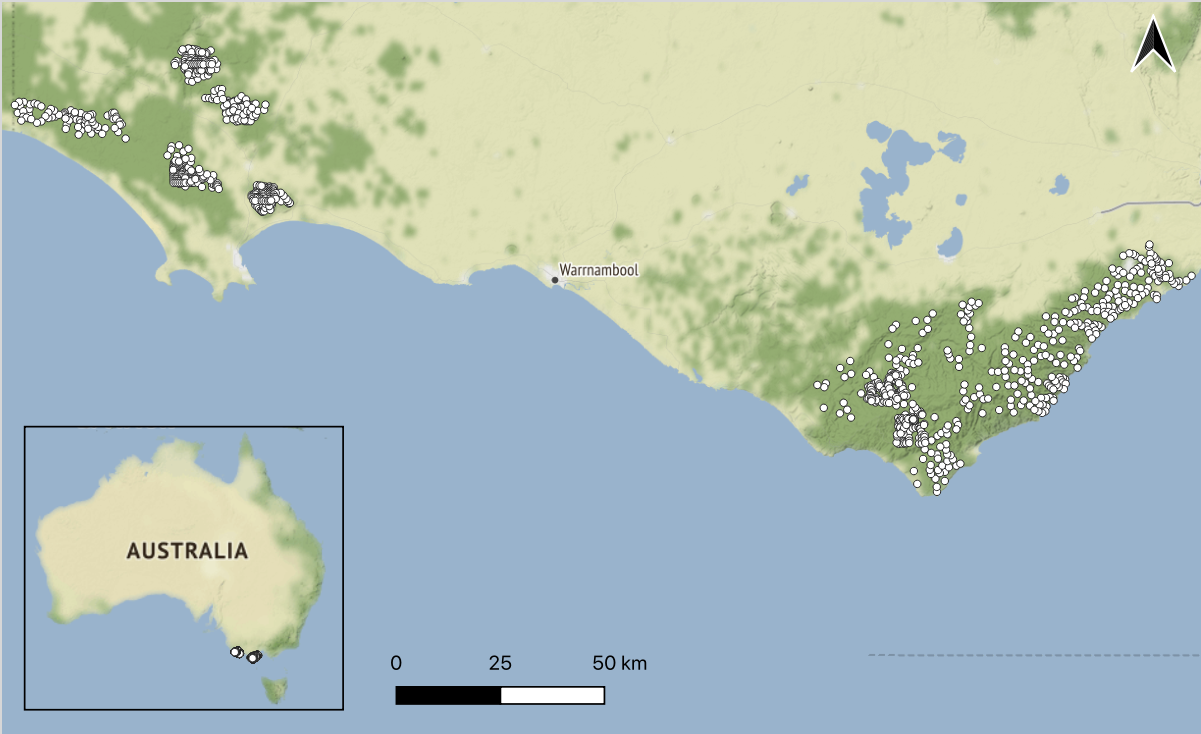
\includegraphics[width=1\linewidth]{figure/map_cams} 

}

\caption{Locations of our study regions in south-west Victoria, Australia. The grids of camera-traps are denoted by white dots. The Glenelg region is to the west and Otway region to the east. Native vegetation is indicated by dark green, with hill shading. \textit{Map tiles by Stamen Design, under CC BY 3.0, map data by OpenStreetMap, under CC BY SA.}}\label{fig:diel-map}
\end{figure}
\newpage

\hypertarget{results-3}{%
\section{Results}\label{results-3}}

Overall, we collated 5449 and 2202 independent detections of foxes and cats, respectively (separated by at least 30 minutes) from 172,052 camera-trap nights (Table \ref{tab:diel-tab1}).

\hypertarget{how-does-predator-overall-activity-and-diel-activity-patterns-vary-across-space-model-1-1}{%
\subsection{How does predator overall activity and diel activity patterns vary across space? (model 1)}\label{how-does-predator-overall-activity-and-diel-activity-patterns-vary-across-space-model-1-1}}

Predator activity varied considerably across space and throughout the 24-hour daily cycle, and there was some variation in the predator diel activity patterns across space. On average, both predators showed similar diel activity patterns: mostly nocturnal with peaks in activity around sunrise and sunset (i.e., crepuscular; Fig. \ref{fig:diel-veg}i). The main difference between the species was that fox activity peaked just after sunset and they were less likely to be active during the day than cats. Cats also tended to be more active at sunset relative to sunrise.

Diel activity pattern strength also differed between the species. Fox activity was concentrated strongly at particular times of the day, especially in the Glenelg region where activity varied by up to 371\% throughout the daily cycle (Fig. \ref{fig:diel-space}a). Feral cats had relatively more consistent activity throughout the daily cycle and across regions; the maximum difference in cat activity throughout the daily cycle for any given location was 185\%.

Variation in diel activity patterns across space, as well as differences in overall activity between the predators, was strongest in the Otway Ranges. For example, overall fox activity (Fig. \ref{fig:diel-space-o-fox}) and diel activity pattern strength(Fig. \ref{fig:diel-space}b) were lowest in the south-west Otway Ranges, while feral cat overall activity (Fig. \ref{fig:diel-space-o-cat}) and diel activity pattern strength (Fig. \ref{fig:diel-space}b) were highest in that subregion.

\hypertarget{how-does-predator-overall-activity-and-diel-activity-patterns-vary-across-vegetation-types-model-2-1}{%
\subsection{How does predator overall activity and diel activity patterns vary across vegetation types? (model 2)}\label{how-does-predator-overall-activity-and-diel-activity-patterns-vary-across-vegetation-types-model-2-1}}

For foxes, little variation in diel activity patterns occurred across any vegetation types except wet forests, where foxes were consistently active throughout the daily cycle (Fig. \ref{fig:diel-veg}a). On the other hand, cats were nocturnal (and most active) in wet forests, but largely crepuscular in all other vegetation types (Fig. \ref{fig:diel-veg}b). For both predators, the random effect for region (Glenelg or Otways) in the vegetation models shrank to near-zero effect, indicating all variation between the regions was explained by the vegetation covariate and site random intercept. Overall levels of fox activity were similar across all EVC groups, except wet forests where fox activity was considerably lower. Relative to foxes, overall cat activity (ignoring diel activity patterns) was more variable across EVC groups; lowest in heathy woodlands and highest in wet forests (Fig. \ref{fig:diel-veg}b).

\hypertarget{do-feral-cats-avoid-foxes-in-space-or-time-model-3-1}{%
\subsection{Do feral cats avoid foxes in space or time? (model 3)}\label{do-feral-cats-avoid-foxes-in-space-or-time-model-3-1}}

Across all habitat type replicates, feral cat diel activity patterns changed across the gradient of fox activity (Fig. \ref{fig:diel-cat-fox}). In the Glenelg region and Otway dry habitat types, feral cats had a nocturnal-crepuscular diel activity pattern where fox activity was low, but were most active during the day where fox activity was high. In contrast, in the wet forests of the Otway Ranges, feral cats were more strongly nocturnal when fox activity was high. Cat spatial activity was relatively unaffected by the fox activity in both habitat types of the Otway Ranges; and, if anything, increased with increasing adjusted fox counts in the Glenelg region (Fig. \ref{fig:diel-cat-fox}), indicating cats did not avoid foxes spatially.

\newpage
\begin{figure}

{\centering 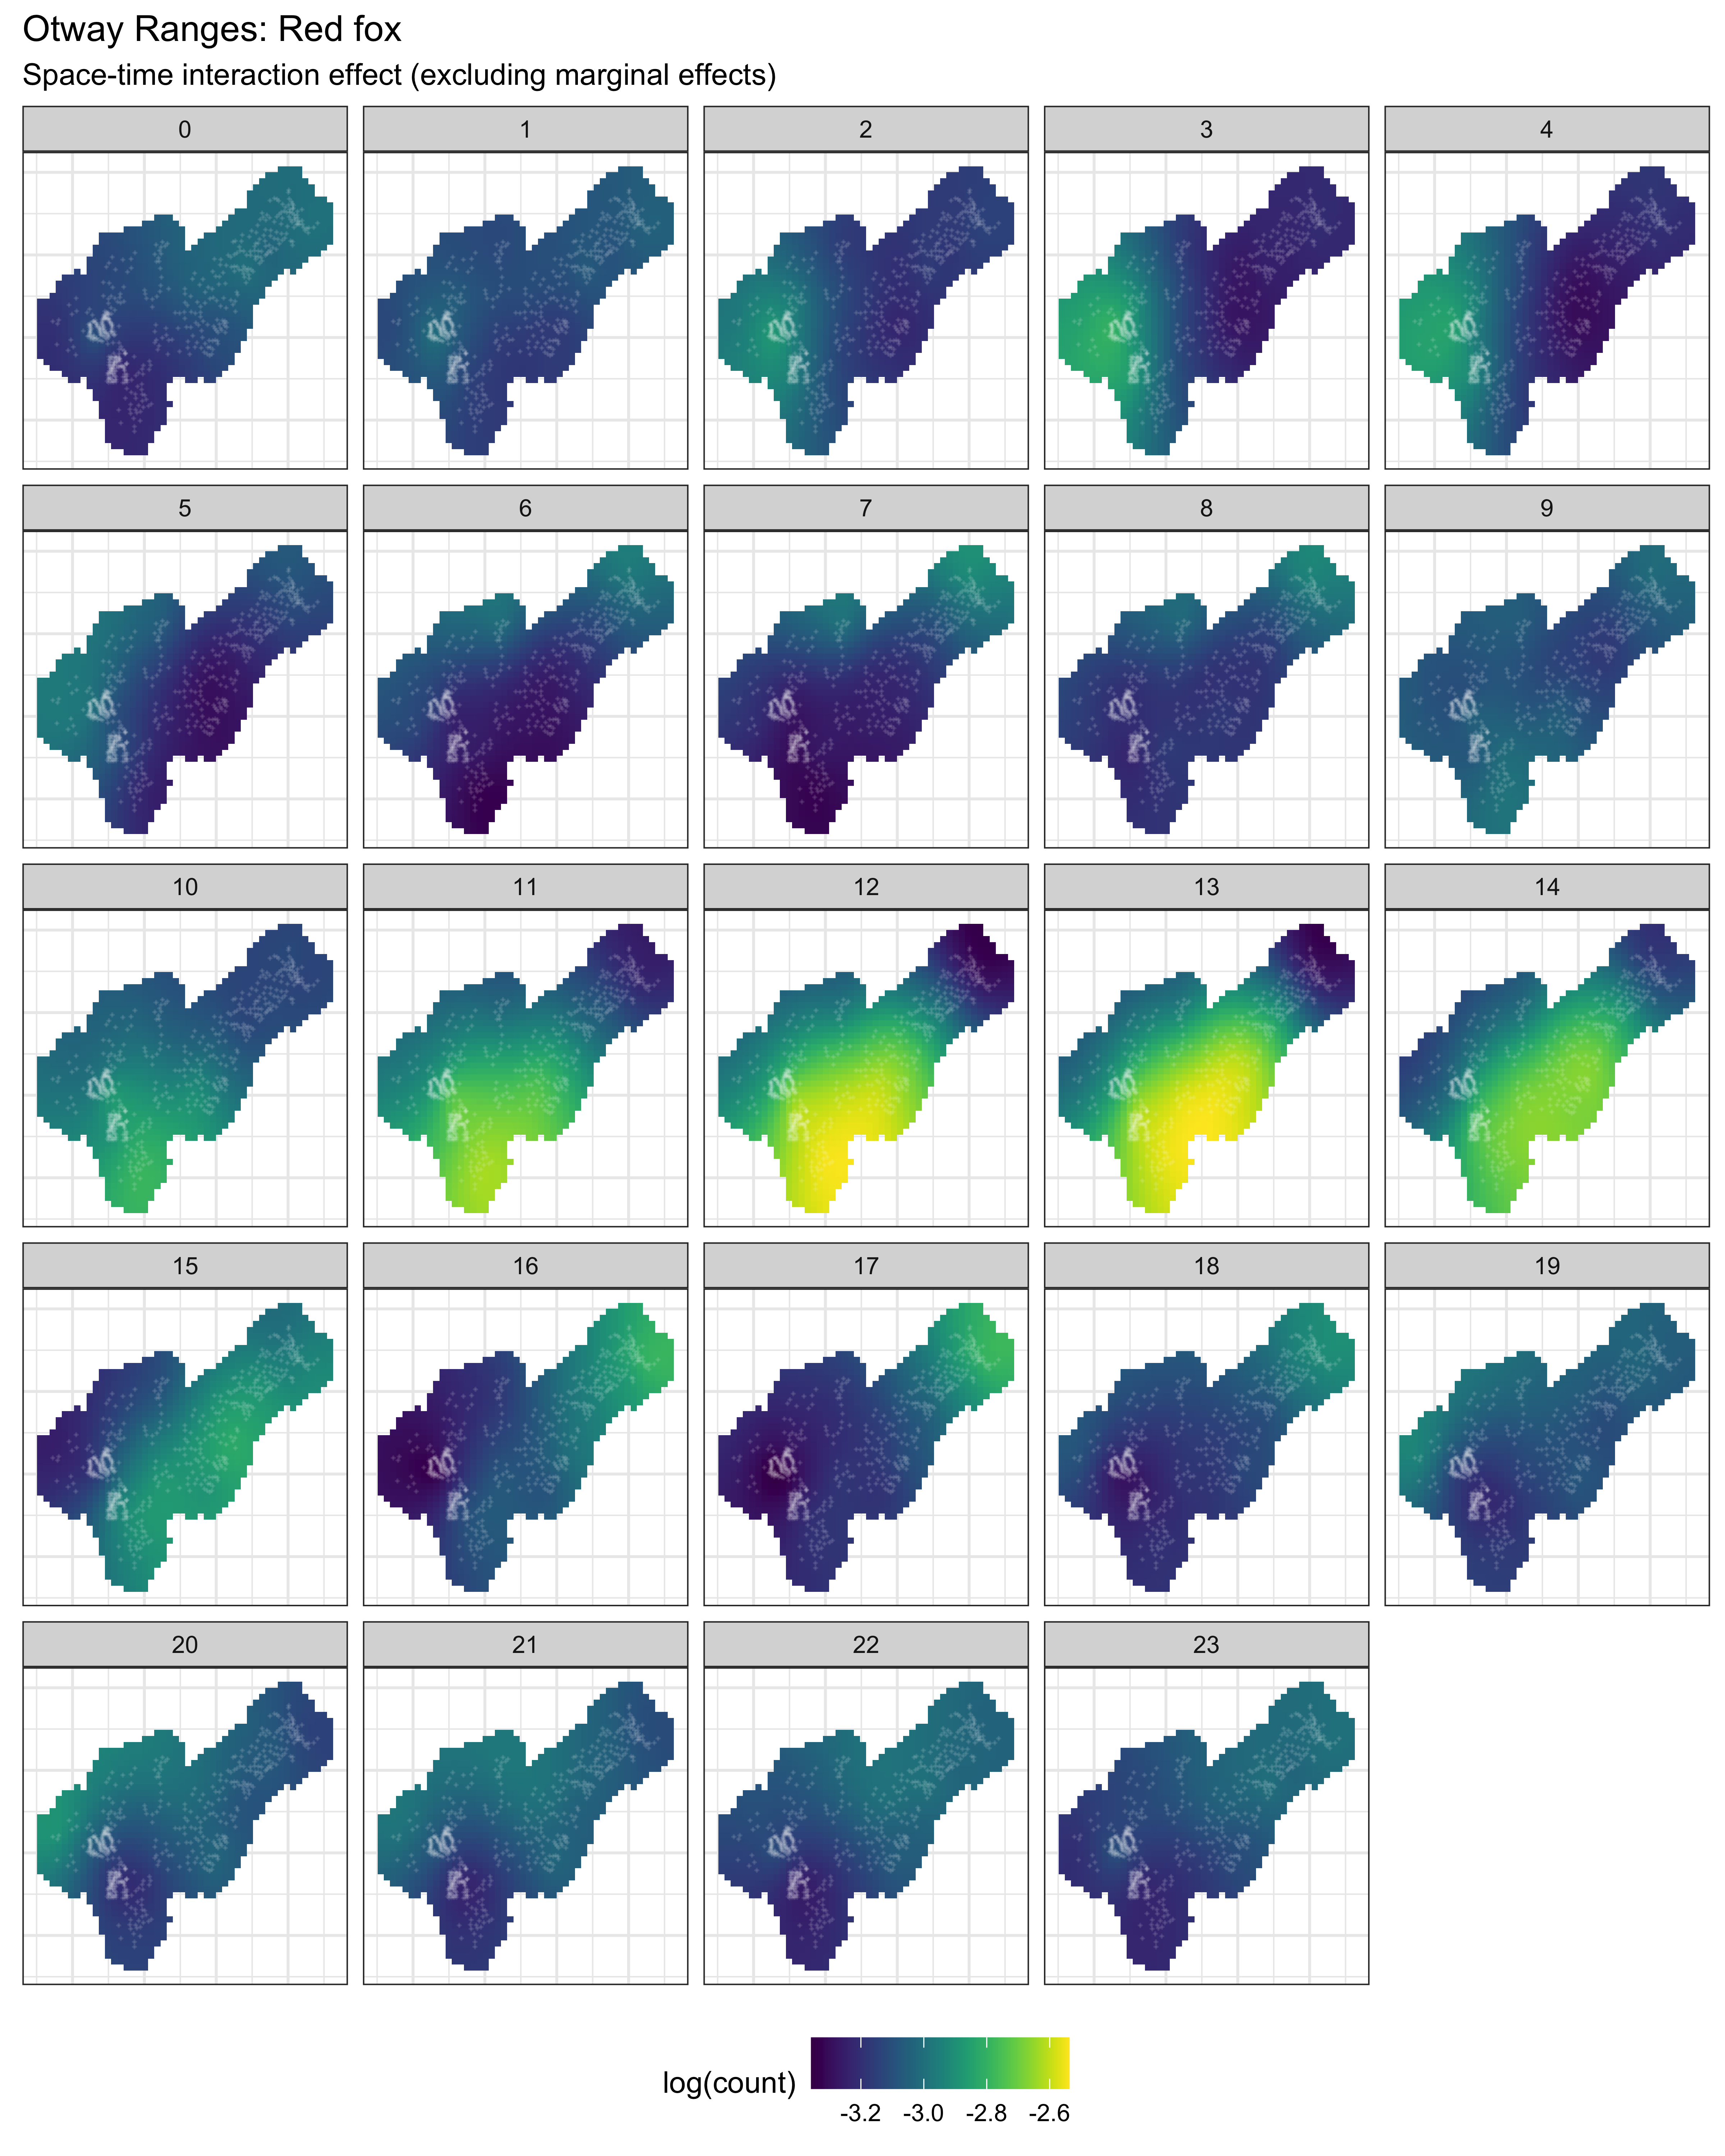
\includegraphics[width=1\linewidth]{figure/spte_diff_avg_o_fox} 

}

\caption{Interaction effect of space-time on red fox \textit{Vulpes vulpes} activity across each hour of the day (0 - 23) in the Otway Ranges, Australia (model 1), as an example. Corresponding plots for feral cats \textit{Felis catus} in this region, as well as both predators in the Glenelg region are provided in the Supporting Information, as are the marginal effects of space and time. White crosses depict unique camera-trap sites.}\label{fig:diel-st-int-o-fox}
\end{figure}
\begin{figure}

{\centering 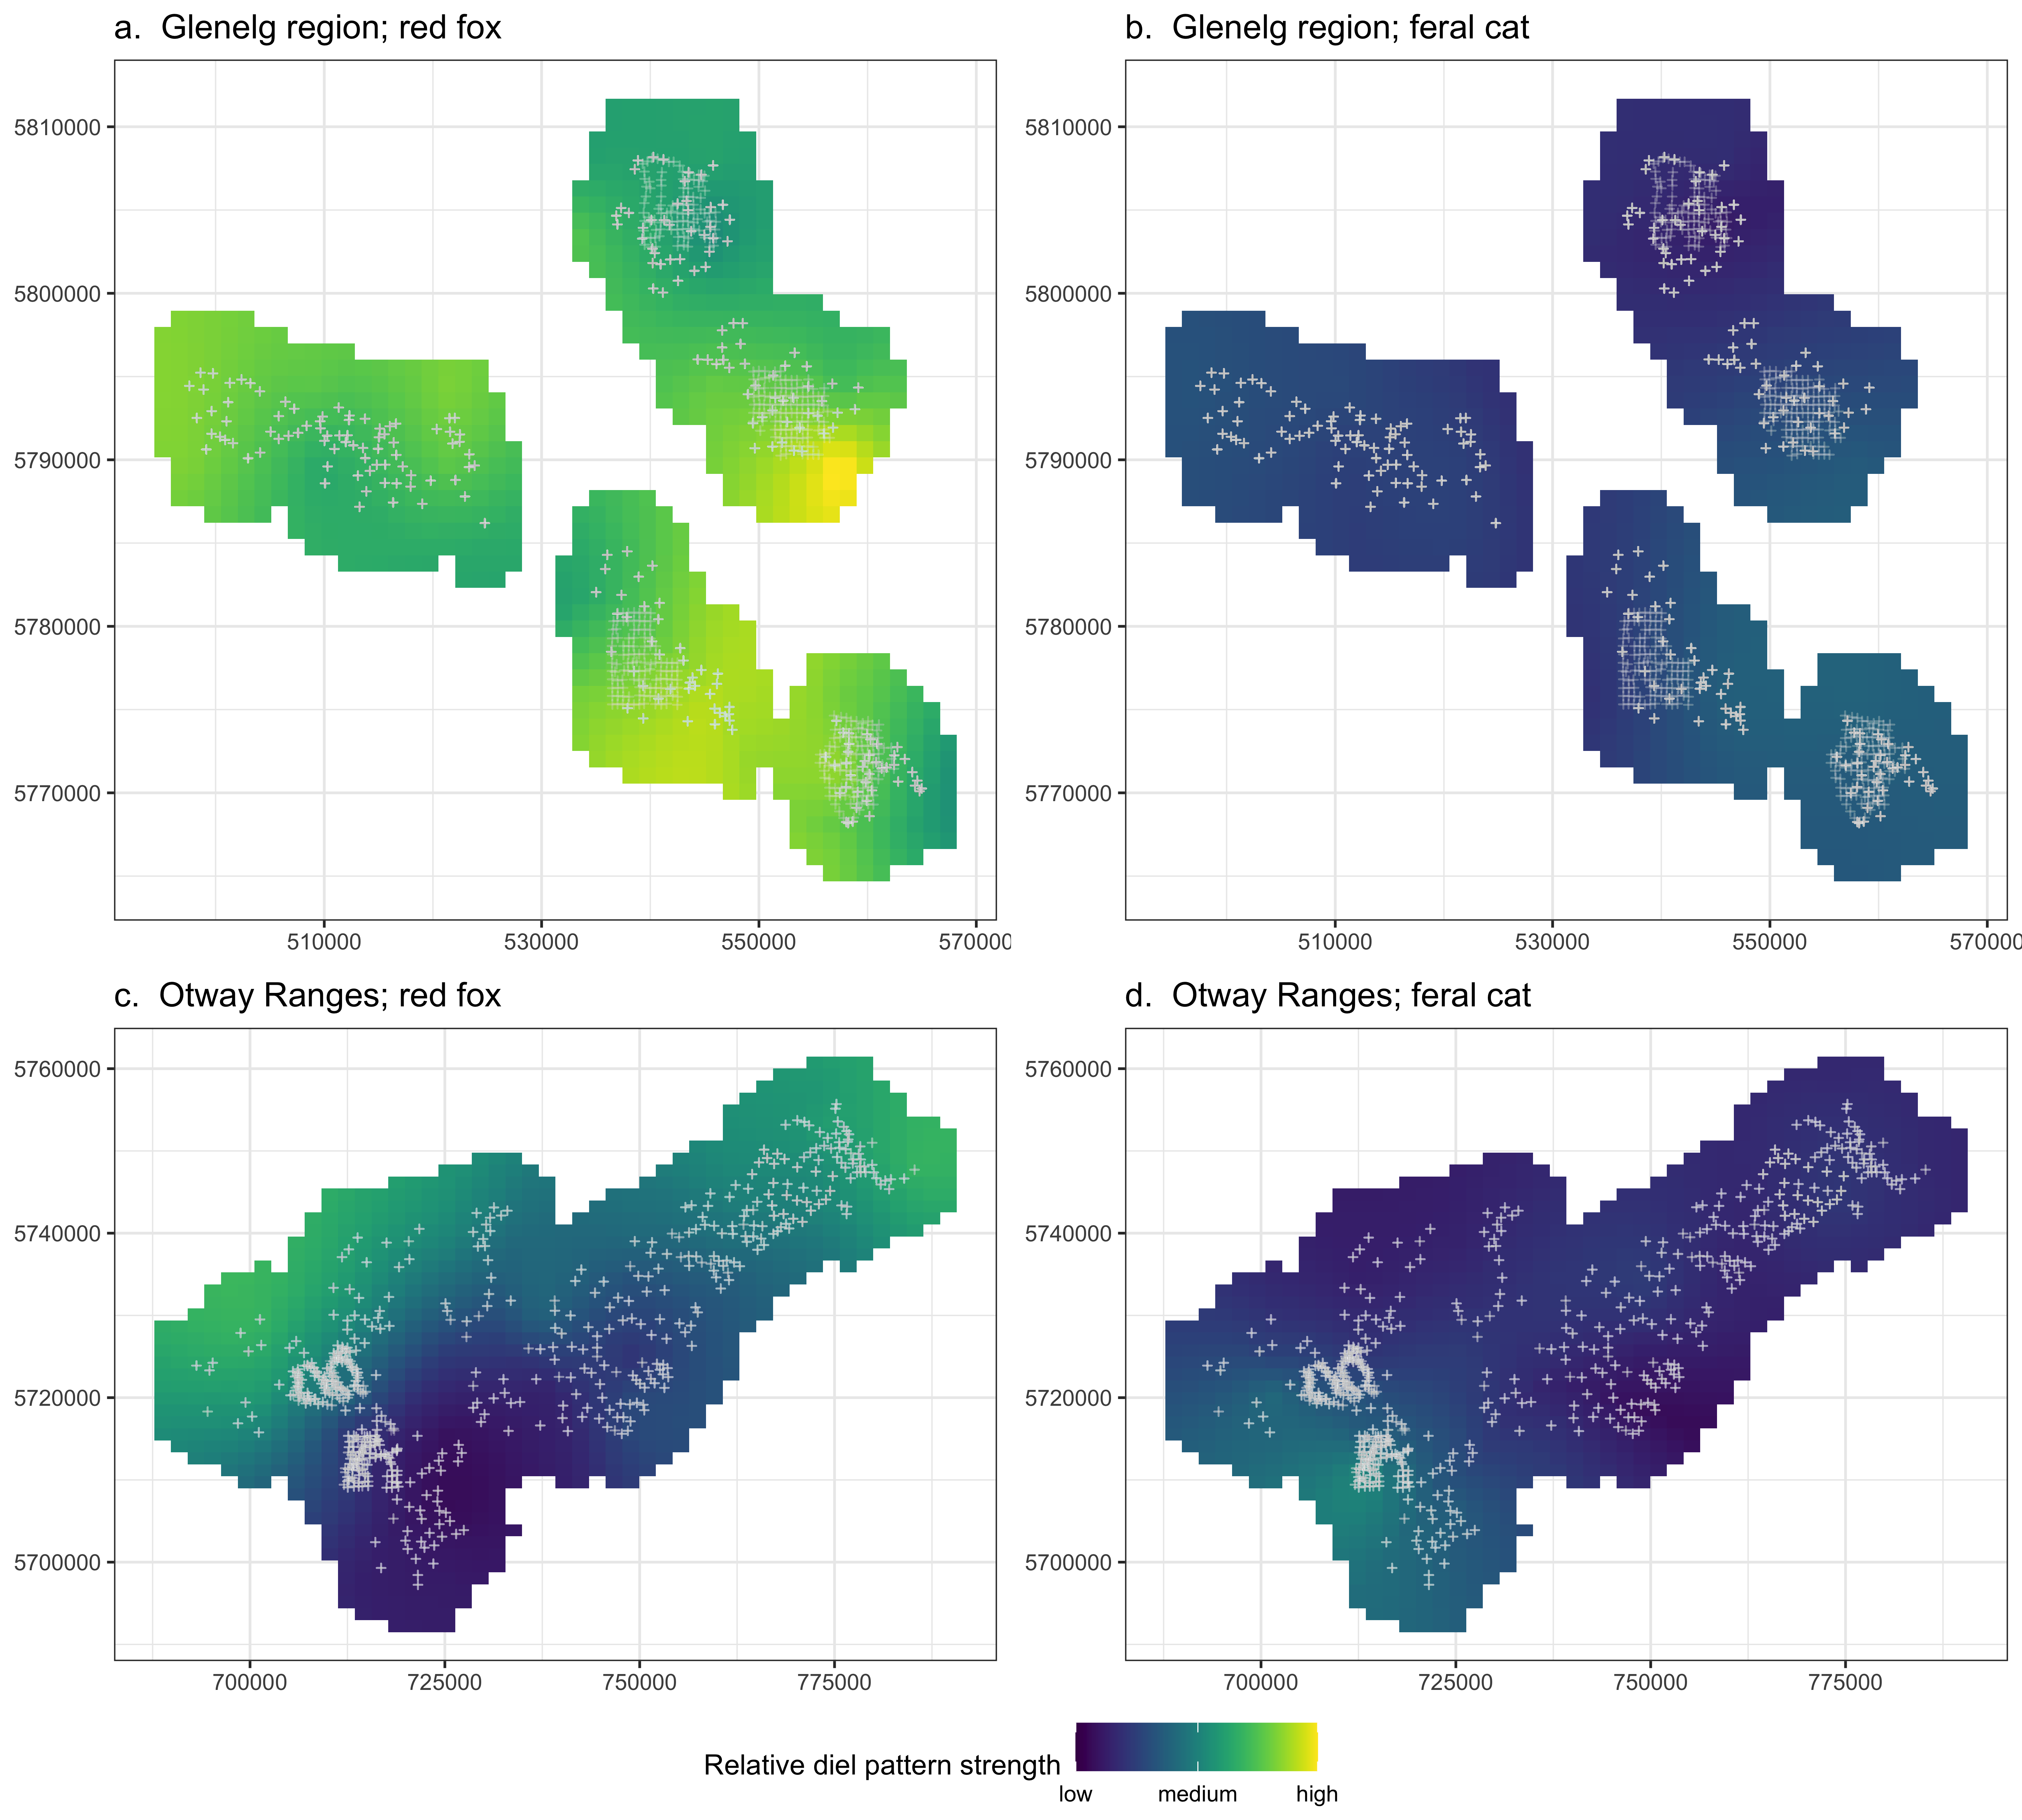
\includegraphics[width=1\linewidth]{figure/diel_strength_600dpi} 

}

\caption{The strength of diel activity patterns of two invasive predators varied within the two study regions in south-west Victoria, Australia (model 1). White crosses depict unique camera-trap sites; colour brightness scales with increasing percentage difference between the minimum and maximum activity estimate over the 24-hour cycle for each location. Red foxes \textit{Vulpes vulpes} (a, c) concentrated their activity during particular times of the day, especially in the Glenelg region (a) and the drier parts of the Otways (c), whereas feral cat \textit{Felis catus} activity was relatively consistent activity throughout the daily cycle (b, d).}\label{fig:diel-space}
\end{figure}
\newpage
\begin{figure}

{\centering 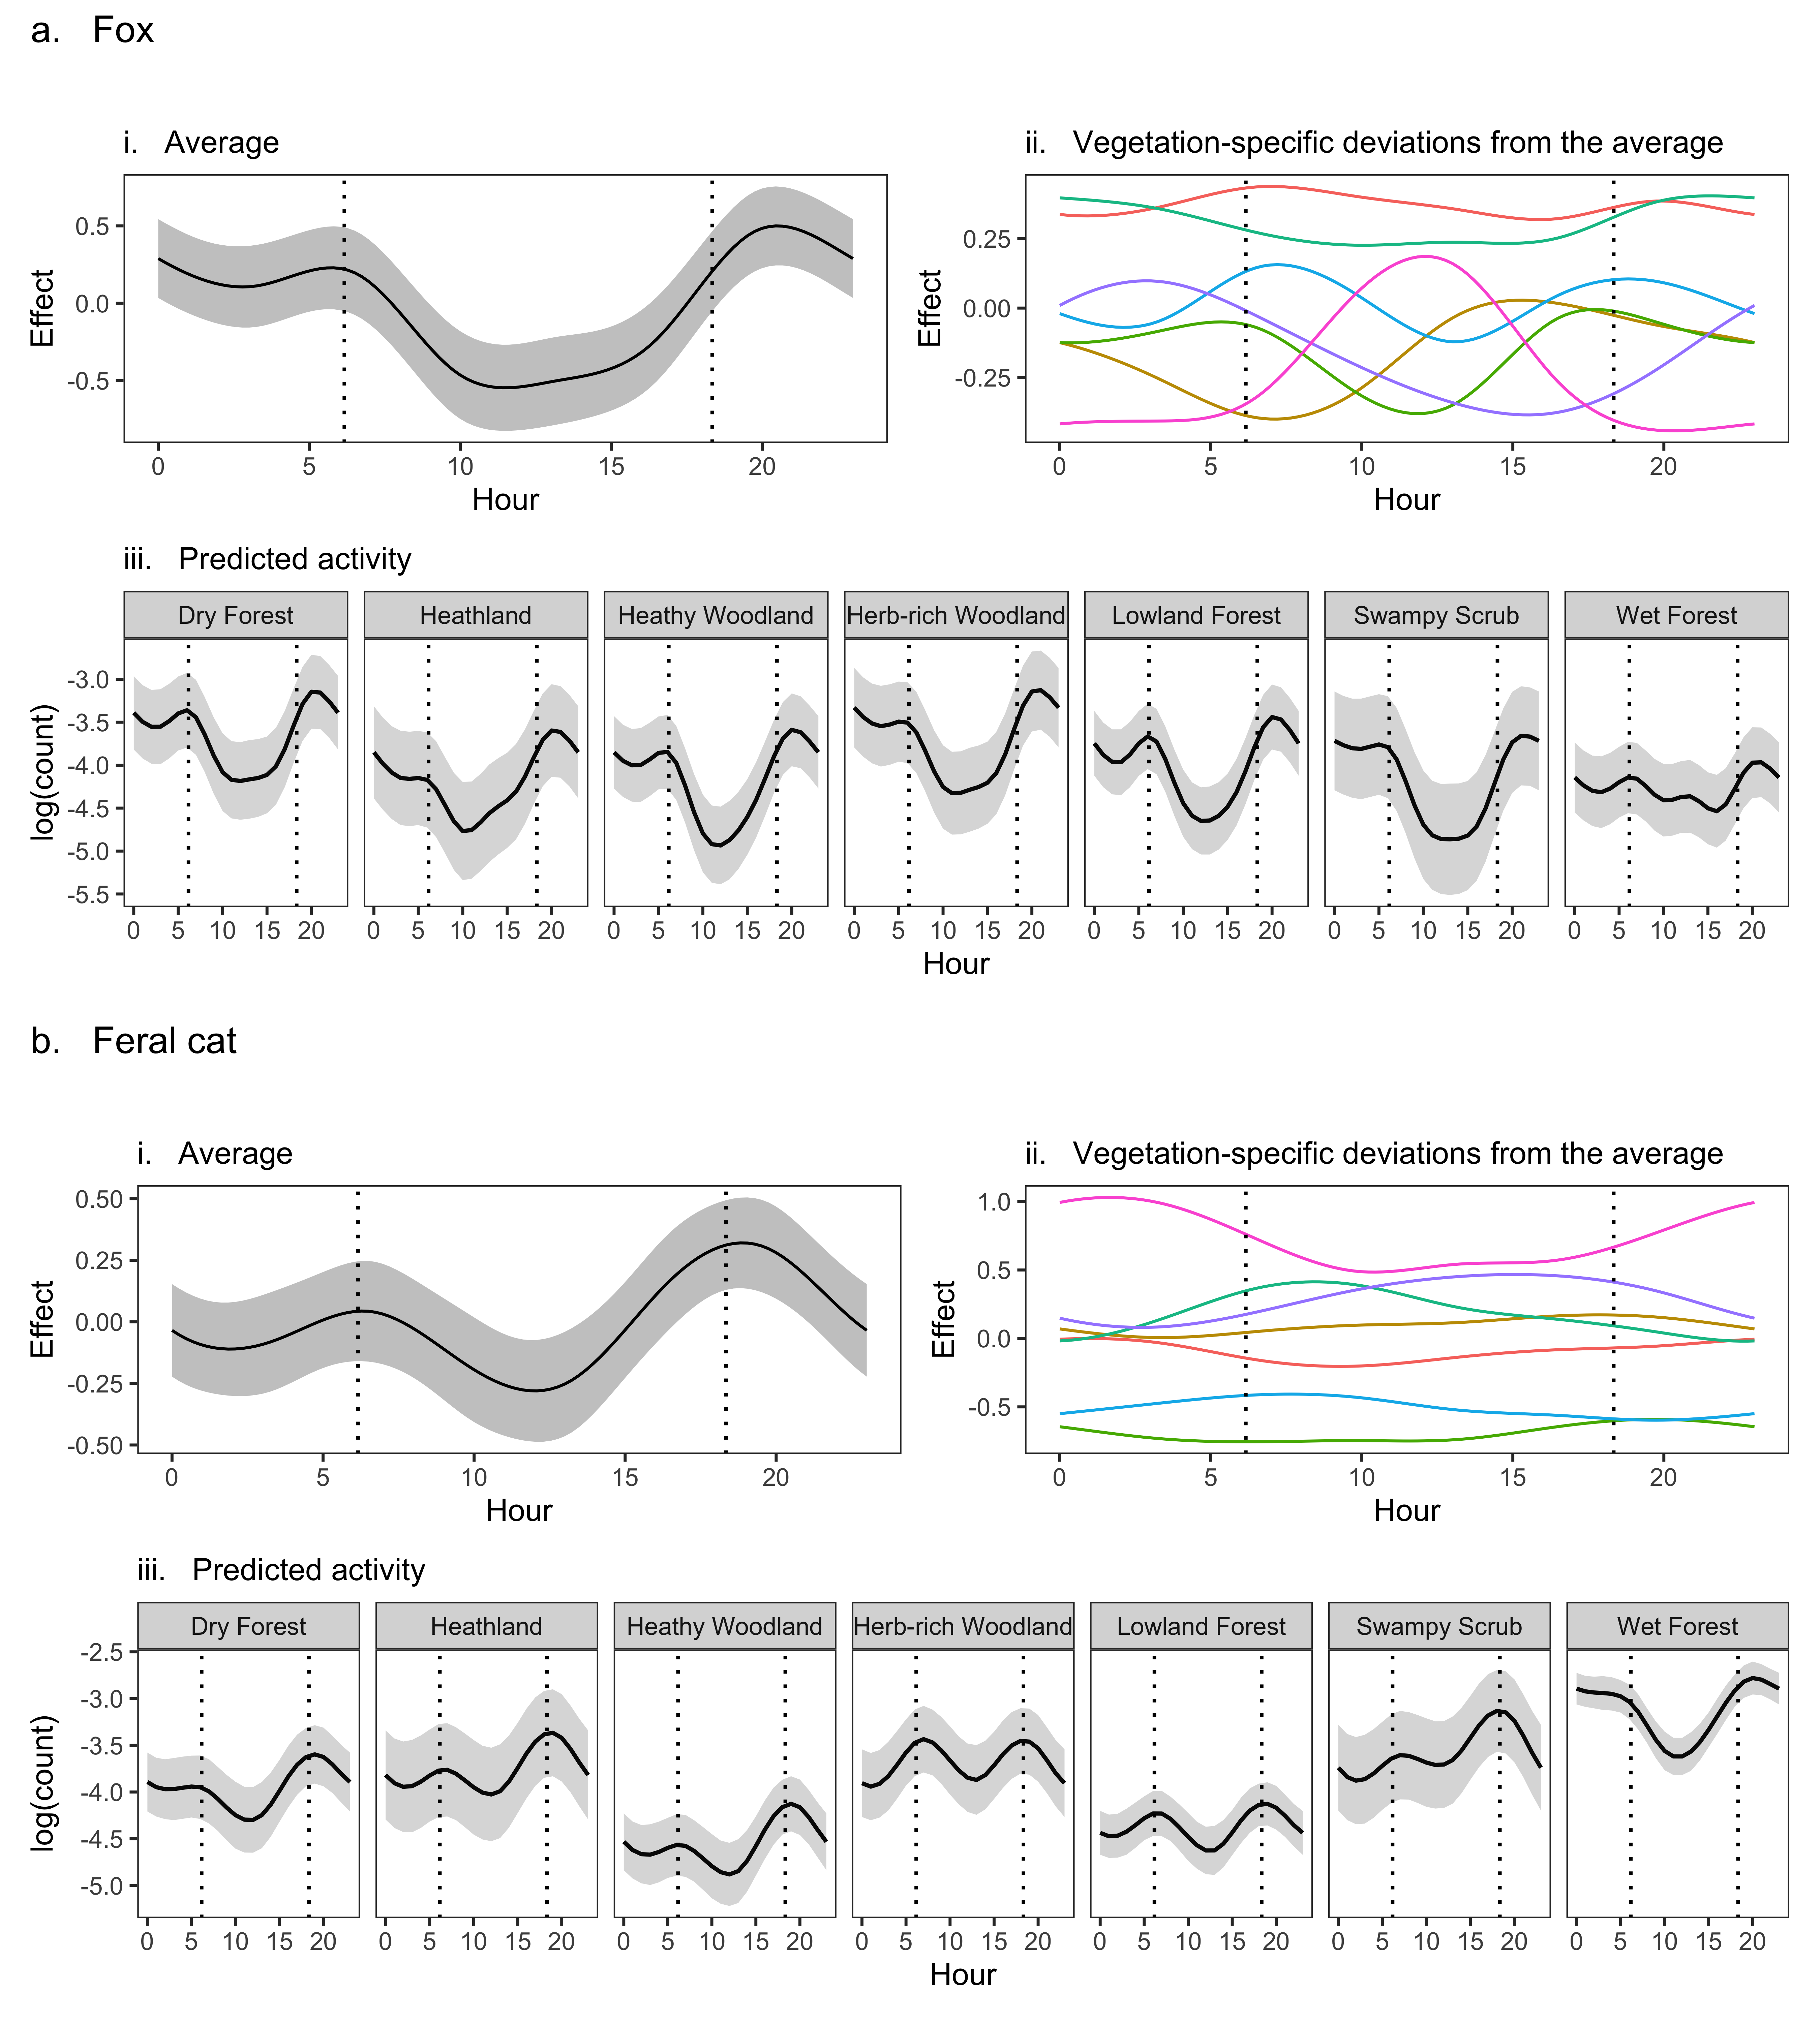
\includegraphics[width=1\linewidth]{figure/predator_veg} 

}

\caption{Red foxes \textit{Vulpes vulpes} (a) and feral cat \textit{Felis catus} (B) diel activity patterns overall (i) and across different Ecological Vegetation Class (EVC) groups (ii, iii) in south-west Victoria, Australia (model 2). Dotted, vertical lines represent average sunrise and sunset times. Shaded areas indicate 95\% confidence intervals. Both invasive predators had a crepuscular to nocturnal diel activity pattern on average, with slight deviations across the drier EVC groups and large deviations in wet forests (ii; wet forests shown as pink line). The overall level of activity was relatively consistent across EVC groups for foxes (a – iii), whereas it differed substantially for feral cats (b - iii).}\label{fig:diel-veg}
\end{figure}
\newpage
\begin{figure}

{\centering 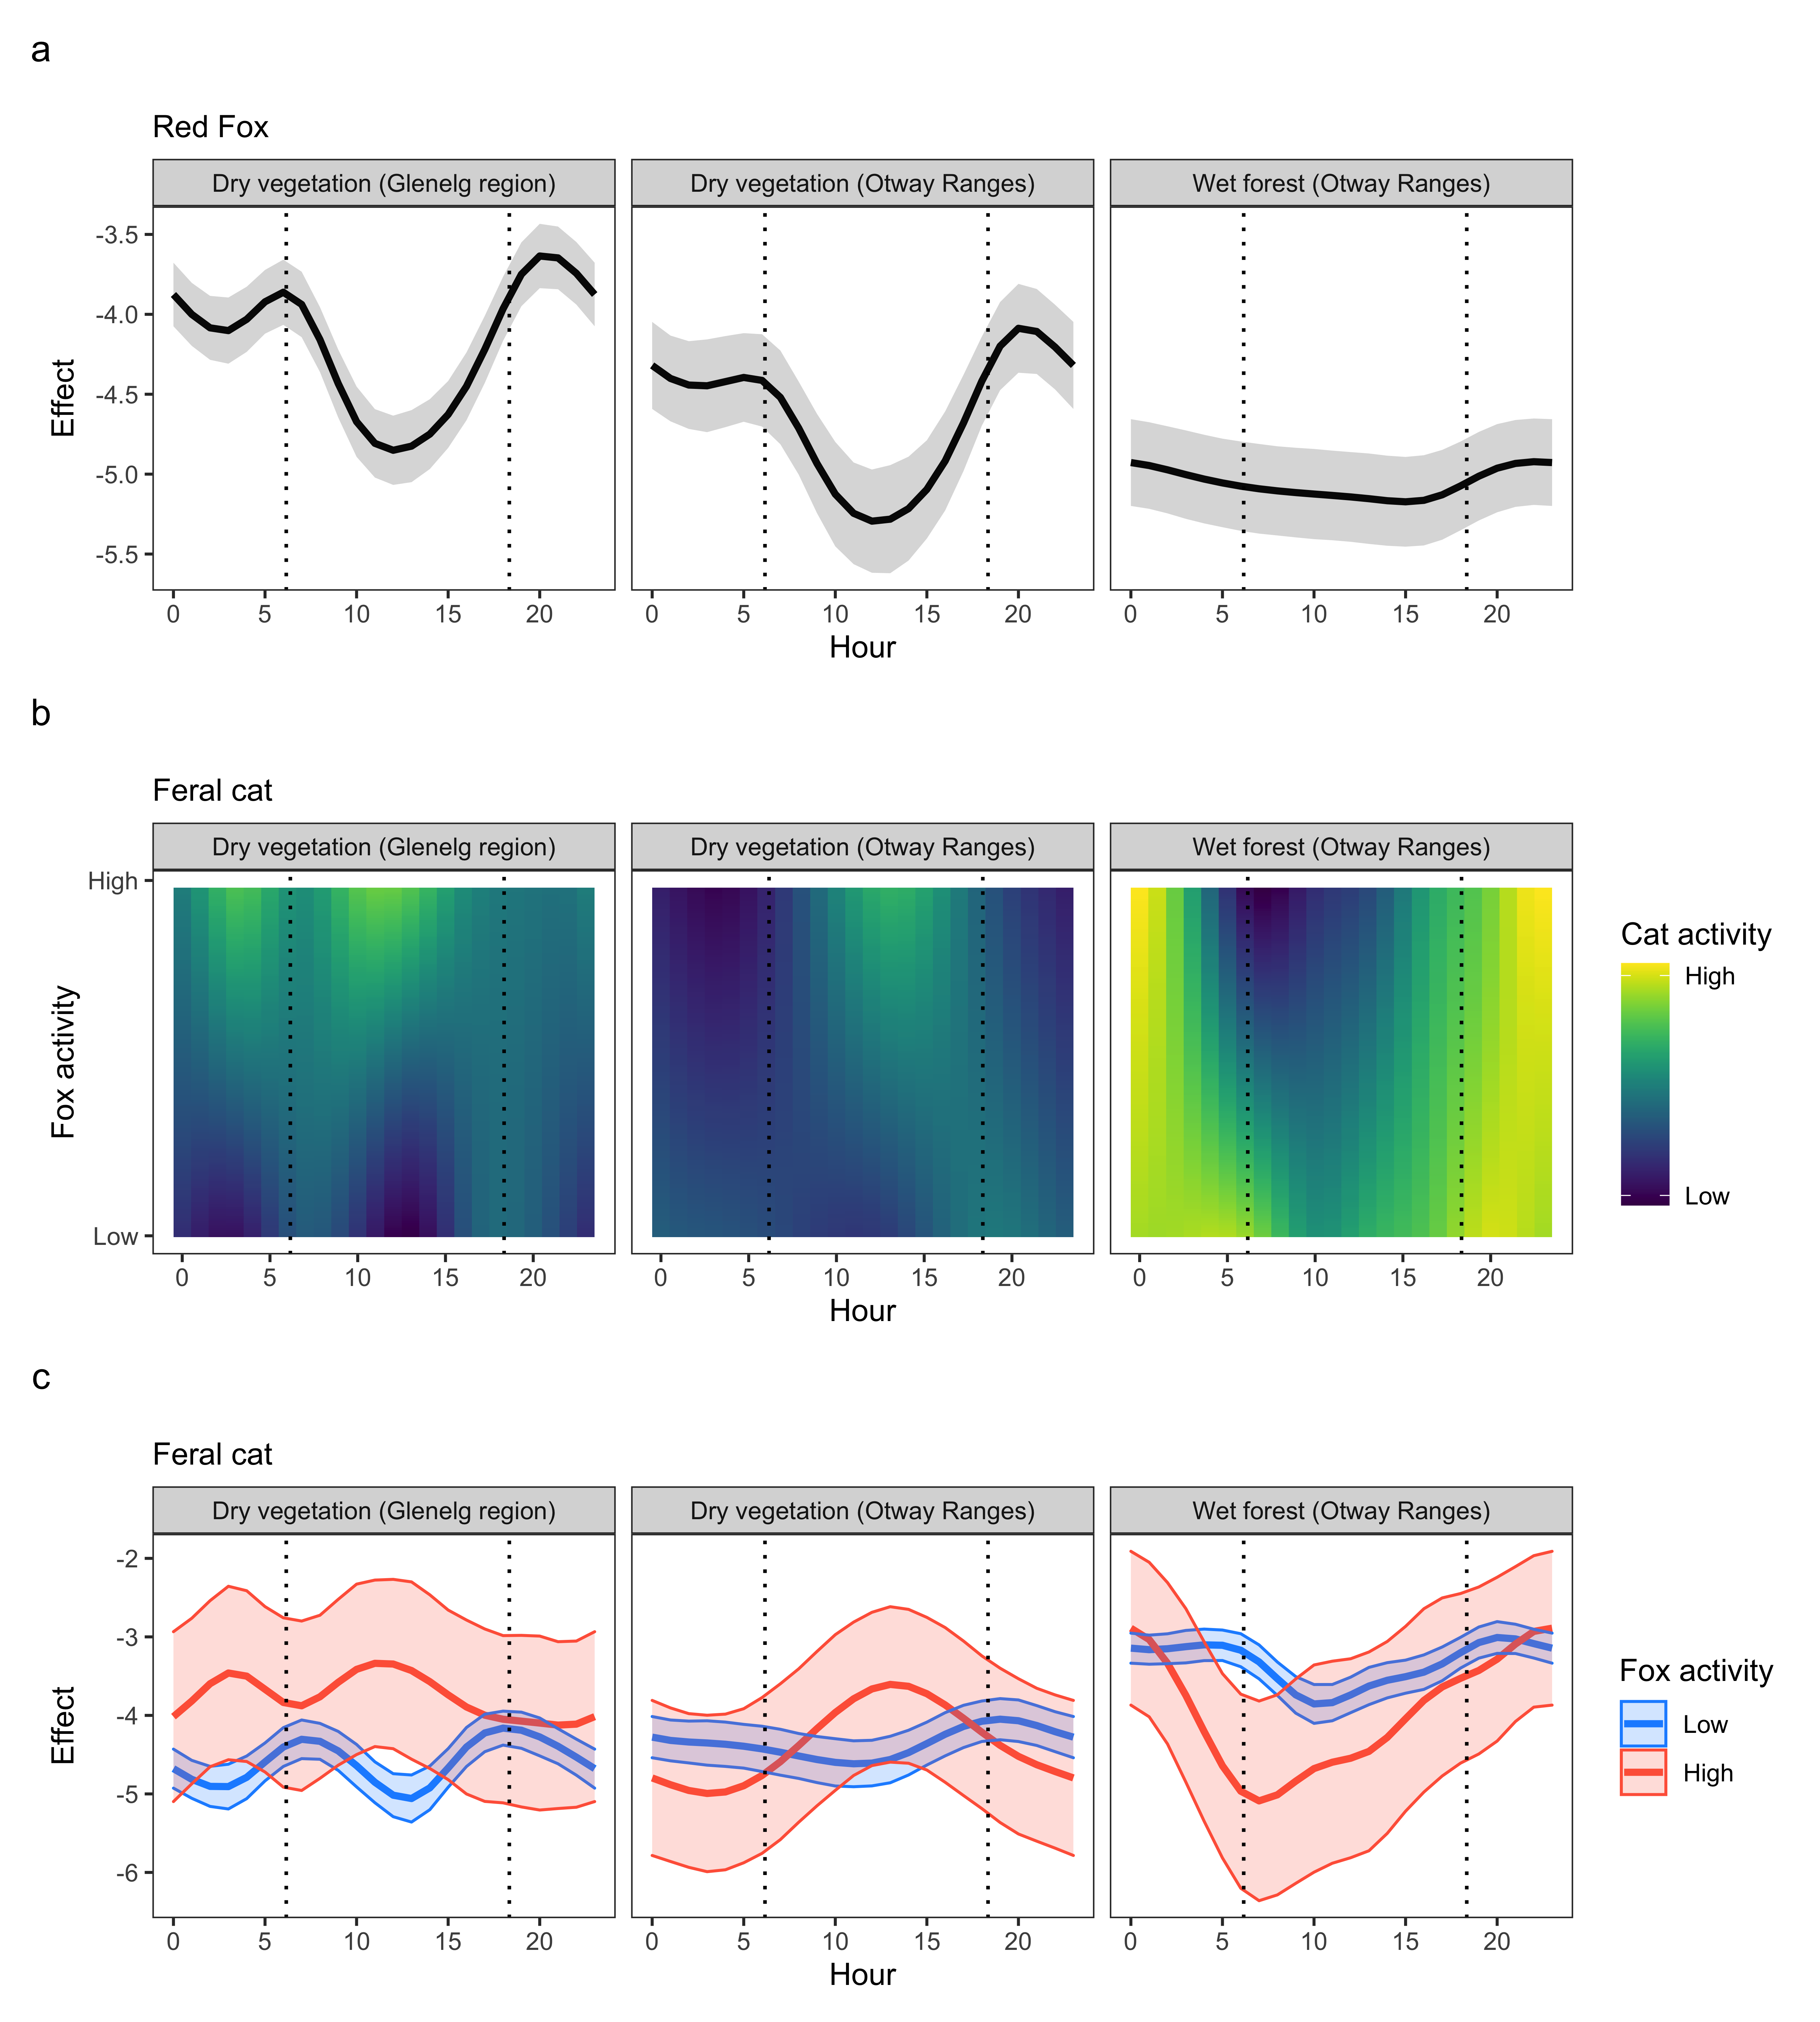
\includegraphics[width=1\linewidth]{figure/cat_fox_count} 

}

\caption{Variation in mean feral cat \textit{Felis catus} activity (a) and associated uncertainty estimates (b) in response to count of ’independent’ red fox Vulpes vulpes detections (log-transformed and survey effort adjusted) across each ’habitat type’ in south-west Victoria, Australia (model 3). Grey vertical lines represent average sunrise and sunset times. In the Glenelg region, there were more feral cat detections where there were more fox detections, but cat peak diel activity shifted from crepuscular night to pre-dawn and midday (a). In the Otway Ranges, feral cat activity also peaked during the day where fox activity was high in dry vegetation types (b), but was more nocturnal where fox activity was high in the rainforests and wet forests (c).}\label{fig:diel-cat-fox}
\end{figure}
\newpage

\hypertarget{discussion-3}{%
\section{Discussion}\label{discussion-3}}

A key question in ecological theory is whether animals are evolutionary hardwired to occupy particular temporal niches, or have circadian rhythms that are responsive to changing environmental conditions and interactions with other species (Schoener 1974; Daan 1981; Lima \& Dill 1990). Here we demonstrate that diel activity patterns are not fixed, but vary across space based on landscape context and fear. In our study, sympatric invasive predators had similar diel activity patterns when averaged across broad regions (i.e., high circular overlap; Fig. \ref{fig:diel-space-time-marginal}; as did Roshier \& Carter 2021), but behaviours varied considerably within landscapes. Fox activity was most strongly tied to the daily cycle in dry habitat types, but showed little diel activity pattern in the wet forests (Fig. \ref{fig:diel-veg}a). In contrast, cats were mostly nocturnal in wet forests and crepuscular in dry vegetation types (Fig. \ref{fig:diel-veg}b). Cats altered diel activity patterns at sites with high fox activity (Fig. \ref{fig:diel-cat-fox}). Reducing invasive fox activity through broadscale lethal control is therefore likely to change cat diel activity patterns, which may shift impacts onto different native prey species. Quantifying changes in diel activity patterns provides important context for understanding species interactions, which is key for effective ecosystem management (Gaynor \emph{et al.} 2021).

Shifting diel activity patterns may allow the spatial coexistence of dominant and subordinate species (Carothers \& Jaksić 1984). For cats, altering preferred diel activity patterns may be worthwhile to persist in high-quality habitat. Few studies have demonstrated predator-induced shifts in diel activity such as these (Kronfeld-Schor \& Dayan 2003), but notably, ship rats \emph{Rattus norvegicus} were also found to switch from nocturnal to diurnal behaviour in response to fox activity (Fenn \& Macdonald 1995). For cats, a switch to diurnal behaviour when fox activity was high in the dry vegetation types in our study regions may have been facilitated by the higher abundance of reptiles relative to wet forests (which are mostly diurnal; Woinarski \emph{et al.} 2018). In the wet forests of the Otway Ranges, cats exposed to high fox activity levels concentrated their activity away from sunrise (mainly) and sunset towards midnight, despite a diurnal shift appearing to similarly reduce the risk of a fox encounter. In this situation, we expect becoming more nocturnal to be favourable over a diurnal shift because this is when the likely preferred prey source (small mammals) are active and cats would be least visible to foxes (as cats here mostly had black or grey coats; Graipel \emph{et al.} 2014). Overall fox activity was also considerably lower in the wet forests relative to dry vegetation types, and so cats were likely under less pressure to radically alter their diel activity patterns. It is unclear why overall fox activity is low in the wet forests and foxes have little diel activity pattern here (Fig. \ref{fig:diel-cat-fox}a). Understanding how these potential behavioural impacts native prey is a key future research priority to improve invasive predator management.

Cats may have avoided foxes in time, but we saw no signs of a fine-scale negative association between fox and cat overall activity (spatial avoidance; (Fig. \ref{fig:diel-cat-fox}b:c). Overlap in spatial activity at fine scales (i.e, at the camera-trap sites) may have been facilitated by temporal avoidance (Kronfeld-Schor \& Dayan 2003). However, we considered spatial avoidance across the entire survey duration (averaging 47 days). Cats may indeed avoid foxes spatially, but transiently on the scale of hours -- days---after all, how is a cat to know where to avoid a fox without encountering signs of one? Short-term spatial avoidance is quite plausible given foxes mark territories using scats and odours, which cats could tangibly associate with high risk shortly after. Temporary spatial avoidance could be tested using decay curves in future research (e.g., Niedballa \emph{et al.} 2019). No sign of spatial avoidance between these invasive predators could also be an artefact of the quality of camera set-up and hence detectability. The 3667 camera-traps were deployed by a range of people, and the quality of set-ups differed considerably in terms of detecting predators. Camera-traps that angled only slightly downwards, rather than upwards or strongly downwards, seemed most effective at detecting both species (M.W Rees, personal observation). Predator interactions are routinely inferred through spatial associations between species, however such analyses are subject to numerous pitfalls which can make inference unreliable (reviewed in Blanchet \emph{et al.} 2020).

A distinction of our study from others is that we modelled potential avoidance behaviours in a simple predator guild, where apex predator activity was artificially manipulated, reducing bias from differences in niche preferences and the unmodelled impacts of other predators in the system. We also included replication across different habitat types, revealing dynamic behavioural responses to apex predators (Fig. \ref{fig:diel-cat-fox}). However, because our study did not consider associations with prey species, we cannot distinguish whether changes in cat diel activity patterns were the result of direct fox avoidance or indirect associations with shared prey. For example, low fox activity may promote the availability of a preferred shared prey species with a diel pattern which differs from those of cats on average, and as a result, cats might shift diel activity patterns at sites with low fox activity to more closely match those of the more abundant prey species. We would expect introduced European rabbits \emph{Oryctolagus cuniculus} (which are diurnal) to be particularly likely to induce such a response in dry vegetation types (McGregor \emph{et al.} 2020; Stobo-Wilson \emph{et al.} 2020a), however, Leporidae species are rare within the natural vegetation landscapes we surveyed (only ever being detected at 40 of 1232 sites) and there is little evidence that predation by foxes suppresses rabbit populations (Norbury \& Jones 2015; Scroggie \emph{et al.} 2018). While of particular interest, whether temporal fox-cat interactions are direct or indirect does not change the resulting impact on native prey, and hence outcome of predator management (fox control).

Flexible antipredator behaviours make evolutionary sense, but have been rarely demonstrated in terms of spatiotemporal predator avoidance (although, see Relyea 2003; Brown \emph{et al.} 2013; Cunningham \emph{et al.} 2019), because this often requires manipulative experiments or at least more complicated models (Kronfeld-Schor \& Dayan 2003). Our study demonstrates that GAMs offer a powerful tool for modelling continuous shifts in animal activity across both space and time, capable of capturing complex interactions and sharing information across categorical variables. The inbuilt smoothing penalties are another benefit of GAMs over kernel density estimation (Ridout \& Linkie 2009), in which noisy data can produce spurious estimates (Frey \emph{et al.} 2017; Iannarilli \emph{et al.} 2019). The alternative approach of simply comparing average diel activity overlap between two species (Ridout \& Linkie 2009) would have been misleading for two reasons. Firstly, predator diel activity patterns varied `naturally' across heterogeneous landscapes (requiring avoidance to be tested in wet forests and dry vegetation types separately; Fig. \ref{fig:diel-veg}). Secondly, apex predator temporal avoidance strategies were not consistently employed, but depended on overall apex predator activity and vegetation type (Fig. \ref{fig:diel-cat-fox}). Despite their underlying statistical complexity, GAMs in the `mgcv' R-package are straightforward to fit. Our GAM framework for modelling spatiotemporal activity can be used on any species with time-stamped detections, including datasets with categorical or continuous covariates and hierarchical groupings.

Animal diel activity patterns can be complex, varying across space, habitat types and threat-levels. Despite telling an important story about how animals interact with each other and the environment, detection times are commonly discarded from statistical analyses of camera-trap data. In the rare instances that they are considered, diel activity patterns are predominantly estimated at the population-level, overlooking finer-scale behaviours that can affect fitness, survival and ecosystem-impacts. Our results demonstrate the importance of (a) considering diel activity in regards to species interactions, (b) modelling \emph{changes} in animal behaviour rather than overlap with other species, and (c) testing avoidance behaviours within a joint spatiotemporal framework. Our study adds to the limited body of evidence that top predators can produce a landscape of fear which is powerful enough to reverse the diel activity patterns of subordinate species (Kronfeld-Schor \& Dayan 2003). Changes in the populations of apex predators may therefore cause a behaviourally mediated trophic cascade.

\hypertarget{synthesis}{%
\chapter{Synthesis}\label{synthesis}}

Does fox control cause mesopredator release of feral cats? This was the central question of my thesis, which I investigated from several different angles. So how do my findings from different population metrics and statistical methods fit together? What should land managers do with this information? And what are the priorities for future research?

\hypertarget{weighing-up-the-evidence-for-mesopredator-release}{%
\section{Weighing up the evidence for mesopredator release}\label{weighing-up-the-evidence-for-mesopredator-release}}

\textbf{The classic definition of the mesopredator release hypothesis (hereafter `MRH') is that an apex predator population decline leads to an increase in the density of mesopredators (Soulé \emph{et al.} 1988), but few studies have tested or demonstrated this}. This is partly due to the difficulty of estimating predator density robustly. By using recently developed spatially explicit capture-recapture methods which allowed for flexible detection rates (Efford 2004), my thesis provides the first evidence that fox control can increase the density of cats. High cat densities were consistently associated with fox control and cat density was negatively associated with fine-scale fox occurrence (Chapter \ref{density}).

The strongest evidence of mesopredator release in terms of population density came from the Glenelg region (Chapter \ref{density}). Fox control in the Glenelg region had occurred for more than a decade, having a strong suppressive effect on fox occupancy (Chapter \ref{occ}). Cat density increased to a smaller extent following fox control commencement in the Otway Ranges, unsurprising given fox control had only recently commenced with less consistent bait replacements. The impact of fox control on cats--ranging from no effect to a nearly four-fold increase in cat density--depended on the degree of fox suppression (Chapter \ref{density}). We confirmed this with regressions between cat density and fox occupancy estimates at fine spatial scales (Fig. \ref{fig:dcor}). Visual inspection of raw estimates suggest cats may respond more closely to foxes at the landscape level--testing predator interactions at different spatial scales would assist in designing future MRH studies (Sivy \emph{et al.} 2017). It is reassuring that fox control was never associated with an estimated decline in cat density (although, 95\% confidence intervals indicates this was possible in some replicates).

While our study provides evidence for the MRH in terms of population density, there are several key limitations. In the Glenelg region, we cannot be sure that feral cat density was not already higher in these landscapes prior to fox control commencing (because there is no available data). I overcame this limitation by using a Before-After-Control-Impact-Paired-Series (BACIPS) design in the western Otway Ranges. However, there was some overlapping of confidence intervals for cat density estimates between treatments in the Otway Ranges experiment, and no spatial replication of the BACIPS design which increasing the vulnerability to type 1 error (i.e., falsely inferring there was an effect of fox control on cats; Conquest 2000).

It would be easy to recommend that managers of new fox control programs conduct spatially replicated, randomised, BACIPS spatial capture-recapture surveys over longer time periods to quantify potential mesopredator release of cats, but difficult to imagine the resources being available to do so. To address the most time-consuming part of this process, collaborators and I have been trialling machine learning methods to automatically identify species and individual cats from camera-trap images; these show promise and are likely to increase the feasibility of such studies by management agencies. Still, reliable estimates from spatial mark-resight models require large sample sizes, which was difficult to obtain for one of the highest density populations of cats on the Australian mainland (Chapter \ref{otways17}). For lower density cat populations, sufficient sample sizes may be more feasibly achieved using clustered spacing of camera-trap over larger areas rather than the grid designs we used (Sun \emph{et al.} 2014; Clark 2019). A key benefit of spatial capture-recapture studies is that differences in study designs can be accounted for, allowing feral cat density estimates to be collated across different landscapes, regions and fox control programs to improve our understanding of fox-cat interactions. This will be particularly important to uncover how different management regimes and landscape contexts impact the strength and occurrence of mesopredator release.

\textbf{Recently, the definition of the MRH has been expanded to also capture changes in mesopredator distribution and behaviour following apex predator decline (Brashares \emph{et al.} 2010)}. I was able to explore these angles using density (Chapter \ref{density}), occupancy (Chapter \ref{occ}) and spatiotemporal activity (Chapter \ref{diel}) models. While changes in cat density in response to fox control were consistent across replicates and regions, changes in cat behaviour and detectability were relatively inconsistent.

The impact of foxes on cat detectability was more reliably observed in the Otway Ranges than the Glenelg region. In the Glenelg region, there was little evidence that cat spatial detection rates changed with fox control or across fox occurrence probability gradients (Chapter \ref{density}). In the Otway Ranges, spatial capture-recapture models revealed that cats did not range as far and were more detectable in their activity centre when fox occurrence was low (Fig. \ref{fig:detcor}); the occupancy-detection model estimated cats to be slightly more detectable with fox control (Fig. \ref{fig:occ-det}a). We also found evidence suggesting cats used behavioural avoidance strategies at low fox occupancy probabilities in the Otway Ranges, which was replaced by reductions in population densities at high fox occurrence probabilities (Fig. \ref{fig:detcor}; Fig. \ref{fig:dcor}. This could explain the lack of avoidance behaviours observed in the Glenelg region, as average fox occurrence probabilities in landscapes with fox control were comparable to the western Otways prior to fox control (Fig. \ref{fig:foxplot}). There is growing recognition of the impact nonconsumptive predator effects can have on ecosystems, a better understanding of what can drive the occurrence and strength of predator avoidance behaviours will be key to accurately predicting the outcomes of predator management (Preisser \emph{et al.} 2005; Wirsing \emph{et al.} 2021).

Differences in landscape context also likely mediate antipredator strategies (Lima \& Dill 1990). Responses vary because of differences in shelter and prey availability, as well as predator density and ecology (Lima \& Bednekoff 1999; Wirsing \emph{et al.} 2021). This was highlighted in Chapter \ref{diel}, which suggested cats avoid foxes in time by becoming more diurnal in dry vegetation types, and more nocturnal in wet forests (Fig. \ref{fig:diel-cat-fox}). These complexities make it difficult to hypothesise how mesopredators will respond to apex predator declines in terms of behaviour--a concern given studies increasingly use behaviour and predator co-occurrences to infer mesopredator release (Jachowski \emph{et al.} 2020). These results demonstrate the importance of comparing responses across a range of contexts, as well as separating out changes in density from behaviour where possible to better understand how mesopredator release manifests.

\textbf{Like many mesopredator release studies that have been conducted using multiple methods across several landscapes (Jachowski \emph{et al.} 2020), I found conflicting inference around predator interactions and the MRH}. The aims of my PhD thesis were similar to those of Molsher (1999), who also found fox control to impact cats in some ways, but not others. Both Molsher (1999) and I found no evidence that fox control increases cat activity indices and evidence that cats may reduce ranging distance following fox control. Coupling telemetry and diet analyses, Molsher (1999) also found cats to increase their use of more open habitat types and consumed more carrion and invertebrates following fox control (Molsher \emph{et al.} 2017). Mesopredator release can manifest in different ways, it is therefore important not to judge mesopredator release on one metric or approach alone.

In my thesis, the most commonly used methods - occurrence models, activity indices, circular overlap in diel patterns (although we did not explicitly test this) - inferred little-no impact of foxes or fox control on cats. Nonetheless, feral cat density increased with fox control (Chapter \ref{density}) and cats shifted diel activity patterns in response to fox activity (Fig. \ref{fig:diel-cat-fox}). There are likely to be several reasons (which I have discussed throughout my chapters) why a higher density of cats did not lead to more sites clearly occupied (Chapter \ref{occ}), and more cat detections (Chapter \ref{diel}), such as changes in behaviour impacting detection rates and facilitating spatial coexistence. Taken together, my results caution the use of simplistic indices to infer density and averaging species responses across broad, heterogeneous regions, and highlight the importance of accounting for changes in detectability when testing the mesopredator release hypothesis.

\textbf{A key source of contention around the MRH is the use of associative rather than causal inference (e.g., Allen \emph{et al.} 2013)}. I used traditional experimental designs as well as (linear and nonlinear) regression methods to test the MRH. Both approaches provided causal inference because foxes were artificially manipulated and fox control was not confounded with other variables (for example, some control programs target effort where predator or prey activity is highest, or only control foxes seasonally). Binary treatments (e.g., fox control) are considered the gold standard in experimental design, but are often imperfect in large scale ecological in-site experiments (Kimmel \emph{et al.} 2021). Testing responses across experimental gradients (e.g., fox occurrence) may be more reliable in certain circumstances, such as when responses are nonlinear (Kreyling \emph{et al.} 2018). I found this to be particularly useful in the Otway Ranges where fox control effort was inconsistent; simplifying fox control into a binary treatment variable overlooked important nuances (e.g., bait density and replacement schedules), which were somewhat irrelevant when fitting a regression between estimated cat density and fox occurrence probabilities. However, the line between causal and associative inference was blurry given I averaged landscapes where foxes were and weren't controlled. Fitting separate regressions to test if inference were consistent across replicates would have been more informative (however I opted against this in my thesis to reduce complexity). Traditional experimental designs are often called for in testing the MRH (e.g., Glen \emph{et al.} 2007; Hayward \emph{et al.} 2015), but are not the only means to provide robust causative inference--a range of experimental approaches can provide complementary inference on management interventions (Kimmel \emph{et al.} 2021).

\textbf{Because we did not compare associations between cats and foxes relative to prey species, we cannot distinguish whether mesopredator release was a result of top-down suppressive or indirect competitive effects}. This is difficult to tease apart, particularly considering direct and indirect mesopredator suppression are both expected to be stronger when intraguild competition is high {[}particularly in depauperate predator guilds; Brashares \emph{et al.} (2010); Prugh \emph{et al.} (2009); Prugh \& Sivy (2020). We did find evidence for direct top-down suppressive effects of foxes on cats through negative correlations between finescale cat density and fox occurrence. Evidence for competitor release would require a negative association between foxes and prey, but would a positive or negative association with cats and prey signal competitor release? A positive association could infer cats track the prey, or be interpreted as coexistence. We currently have a poor understanding of how prey availability impacts cat density (Legge \emph{et al.} 2017), particularly in temperate regions relative to the arid and semiarid (e.g., {\textbf{???}}).

My thesis provides evidence that foxes can constrain the population density and temporal activity patterns of feral cats in temperate, meeting the definitions of mesopredator release (Prugh \emph{et al.} 2009; Brashares \emph{et al.} 2010; Jachowski \emph{et al.} 2020). We found signs of other behavioural changes, such as differences in movement and detection rates, but these were observed relatively inconsistently. Predicting behavioural changes in mesopredator behaviour following apex predator decline will be a key challenge for future research. Advancing the MRH will require surveying mesopredator responses a range of landscape contexts, with the use of different experimental and analytical methods.

My thesis provides evidence that fox control can cause a mesopredator release of feral cats, a result which should encourage integrated invasive predator control. However, where simultaneous or staggered control of foxes and cats is not feasible, managers need to weigh up the benefits of reducing fox predation against potentially increasing cat predation of vulnerable fauna to accurately assess the net benefit of fox control for biodiversity conservation.

\hypertarget{does-a-mesopredator-release-of-feral-cats-matter}{%
\section{Does a mesopredator release of feral cats matter?}\label{does-a-mesopredator-release-of-feral-cats-matter}}

Based on cat density estimates (Legge \emph{et al.} 2017) and diet analyses, Australian feral cats are estimated to kill 1.4 billion native Australian animals each year (Woinarski \emph{et al.} 2017, 2018; Murphy \emph{et al.} 2019). However, predation rates of particular species may not necessarily increase with cat population density. This is because predation rate depends on cat demographics (Moseby \emph{et al.} 2015), individual specialisation (Dickman \& Newsome 2015), as well as predator and prey behaviour (Abrams 1993) and microhabitat context (McGregor \emph{et al.} 2015a). Only a small number of cats are required to inflict large damage to local populations (Greenwell \emph{et al.} 2019; Moseby \emph{et al.} 2019; Tuft \emph{et al.} 2021).

Cats have been implicated in the extinction of many Australian species, most notably in northern Australia (where foxes are absent; Woinarski \emph{et al.} 2015; Davies \emph{et al.} 2018; Stobo-Wilson \emph{et al.} 2020c). However, cat densities in northern Australia are low (Stokeld \emph{et al.} 2016; Legge \emph{et al.} 2017; McGregor \emph{et al.} 2017; Davies \emph{et al.} 2021). The prevailing hypothesis to explain this is that fire and large herbivore grazing have reduced understorey habitat structure, thereby increasing cat predation rates (Ziembicki \emph{et al.} 2015). However, perhaps feral cats did reach unsustainably high densities in northern Australia, enabled by the once-abundant fauna populations and lack of suppression from foxes, leading to prey population crashes and subsequently their own. The possibility of this boom-bust cat-prey dynamic is a concern for the Otway Ranges, where cat density is among the highest in Australia (Chapter 2) and small mammal species have declined in recent times (Menkhorst \& Broome 2006; Lock \& Wilson 2017; Wayne \emph{et al.} 2017b; Wilson \emph{et al.} 2017; Wilson \& Garkaklis 2020). There is extremely limited information on temporal trends in cat densities, my three-year study in the Otway Ranges offers an important baseline for future comparison. Understanding how cat density fluctuates over time and how this relates to prey populations is a priority for future research.

Behavioural traits are likely strong drivers of predation, although more difficult to understand relative to predator density (Abrams 1993).

The primary aim of this thesis was to understand whether mesopredator release occurring rather than its implications for native fauna. Nonetheless, fox control has now been shown to alter the density, diel activity patterns, movement-rates, habitat preferences and diets of cats (Molsher \emph{et al.} 2017). It is therefore plausible to expect that fox control will increase the impact of feral cats, but also potentially also shift impacts onto different species or individuals which have previously had less exposure cat predation. Furthermore, I was able to examine the responses of two shared native prey. These potential impacts of a mesopredator release may explain why southern brown bandicoots showed no increase in sites occupied following fox control. However, long-nosed potoroos have strongly benefited from fox control in the Glenelg region (but not the Otway Ranges).

Some native prey, particularly larger species, are more more susceptible to foxes than cats (Stobo-Wilson \emph{et al.} 2021a, b; Woinarski \emph{et al.} 2021). For example, a density of 0.03 foxes km\textsuperscript{-2} drove a reintroduced population of burrowing bettongs \emph{Bettongia lesueur} to extinction within 12 months, but another population persisted with no foxes and up to 0.46 cats km\textsuperscript{-2} (Moseby \emph{et al.} 2019). There is not statistical evidence that prey weight on which species benefit from fox control, although species such as rodents and small dasyurids have been far less often monitored (Hunter \emph{et al.} 2018), and are most likely to be impacted from a mesopredator release of cats. For example, bush rats \emph{Rattus fuscipes} have been reported as receiving no benefit (Banks 1999) as well as becoming locally extinct following fox control (Wayne \emph{et al.} 2017a). Further, prey can be driven by both bottom-up and top-down effects and the relative importance of these processes can vary geographical and temporally, making it difficult to predict how changes in predator populations will impact prey (Sinclair \emph{et al.} 1998; Oksanen \& Oksanen 2000; Sinclair \& Krebs 2002; Meserve \emph{et al.} 2003). More work is needed to examine the responses of different prey species to fox control, particularly smaller species which are more likely sensitive to cat predation.

Threats can act in synergy. If fox control leads to both a release of cats and herbivores, this could reduce habitat structure which would increasing vulnerability of prey to cats and any surviving foxes. There is concern that large macropods (kangaroos and wallabies) may become overabundant following fox control (as foxes are their primary terrestrial predators where dingoes are absent), thereby increasing their grazing pressure which could reduce the habitat structure smaller prey species require to shelter in (Doherty \& Ritchie 2017). There is some evidence for this (Banks \emph{et al.} 2000). Additionally, there is concern in the Glenelg region that an increase in common brush-tailed possums has potentially excluded threatened native prey from sites (such as tree hollows). However, Geary \emph{et al.} (2020b) modelled the effect of fox control of medium-large herbivore with the Glenelg Ark dataset and found no effect of fox control on herbivore occurrence. Nonetheless, herbivore release could still manifest from changes in herbivore density, recruitment rates and behaviour, therefore worth further investigation.

These factors make it difficult to predict what impact a mesopredator release of feral cats will have on native prey of concern. Even with mesopredator release of feral cats, fox control has value as a conservation action (Hunter \emph{et al.} 2018). However, fox control programs are rarely monitored in ways which can reliably detect which species are responding positive, neutrally or negatively to fox control. I hope my thesis does not discourage the use of targeted fox control but encourages the careful monitoring of feral cats and a wider range of shared prey taxa (particularly species that might be highly vulnerable to cats). If cat density increases considerably, or particularly species show signs of decline, lethal cat control should be integrated (e.g., Comer \emph{et al.} 2020). Indirect predator management {[}e.g.~rabbit control{]} or more targeted species-specific conservation actions {[}e.g.~tailored fire management{]} could also be employed. In dire situations, fox control could be ceased, however this would lose the earlier value of fox control -- and fox control needs to be sustained over the longer-term.

\hypertarget{references}{%
\chapter*{References}\label{references}}
\addcontentsline{toc}{chapter}{References}

\markboth{References}{References}

\noindent

\setlength{\parindent}{-0.20in}
\setlength{\leftskip}{0.20in}

\hypertarget{refs}{}
\leavevmode\hypertarget{ref-abbott2008spread}{}%
Abbott, I. (2008). The spread of the cat, \emph{felis catus}, in Australia: Re-examination of the current conceptual model with additional information. \emph{Conservation Science Western Australia}, 7.

\leavevmode\hypertarget{ref-abrams1993predation}{}%
Abrams, P.A. (1993). Why predation rate should not be proportional to predator density. \emph{Ecology}, 74, 726--733.

\leavevmode\hypertarget{ref-algar2020feral}{}%
Algar, D., Johnston, M., Tiller, C., Onus, M., Fletcher, J. \& Desmond, G. \emph{et al.} (2020). Feral cat eradication on Dirk Hartog Island, Western Australia. \emph{Biological Invasions}, 22, 1037--1054.

\leavevmode\hypertarget{ref-allen2017can}{}%
Allen, B.L., Allen, L.R., Andrén, H., Ballard, G., Boitani, L. \& Engeman, R.M. \emph{et al.} (2017). Can we save large carnivores without losing large carnivore science? \emph{Food Webs}, 12, 64--75.

\leavevmode\hypertarget{ref-allen2013clear}{}%
Allen, B.L., Fleming, P.J.S., Allen, L.R., Engeman, R.M., Ballard, G. \& Leung, L.K.-P. (2013). As clear as mud: A critical review of evidence for the ecological roles of Australian dingoes. \emph{Biological Conservation}, 159, 158--174.

\leavevmode\hypertarget{ref-alston2019reciprocity}{}%
Alston, J., Maitland, B., Brito, B., Esmaeili, S., Ford, A. \& Hays, B. \emph{et al.} (2019). Reciprocity in restoration ecology: When might large carnivore reintroduction restore ecosystems? \emph{Biological conservation}, 234, 82--89.

\leavevmode\hypertarget{ref-arjo2007changes}{}%
Arjo, W.M., Gese, E.M., Bennett, T.J. \& Kozlowski, A.J. (2007). Changes in kit fox--coyote--prey relationships in the Great Basin Desert, Utah. \emph{Western North American Naturalist}, 67, 389--401.

\leavevmode\hypertarget{ref-arthur2012relative}{}%
Arthur, A.D., Catling, P.C. \& Reid, A. (2012). Relative influence of habitat structure, species interactions and rainfall on the post-fire population dynamics of ground-dwelling vertebrates. \emph{Austral Ecology}, 37, 958--970.

\leavevmode\hypertarget{ref-baker2017ensemble}{}%
Baker, C.M., Gordon, A. \& Bode, M. (2017). Ensemble ecosystem modeling for predicting ecosystem response to predator reintroduction. \emph{Conservation Biology}, 31, 376--384.

\leavevmode\hypertarget{ref-baker2004polygynandry}{}%
Baker, P.J., Funk, S.M., Bruford, M.W. \& Harris, S. (2004). Polygynandry in a red fox population: Implications for the evolution of group living in canids? \emph{Behavioral Ecology}, 15, 766--778.

\leavevmode\hypertarget{ref-ballari2016potential}{}%
Ballari, S.A., Kuebbing, S.E. \& Nuñez, M.A. (2016). Potential problems of removing one invasive species at a time: A meta-analysis of the interactions between invasive vertebrates and unexpected effects of removal programs. \emph{PeerJ}, 4, e2029.

\leavevmode\hypertarget{ref-banikos2018responses}{}%
Banikos, Z. (2018). Responses of critical weight range digging mammals to a fox control program in south-eastern Australia. Master's thesis. University of Melbourne; School of BioSciences.

\leavevmode\hypertarget{ref-banks1999predation}{}%
Banks, P.B. (1999). Predation by introduced foxes on native bush rats in Australia: Do foxes take the doomed surplus? \emph{Journal of Applied Ecology}, 36, 1063--1071.

\leavevmode\hypertarget{ref-banks2000predation}{}%
Banks, P.B., Newsome, A.E. \& Dickman, C.R. (2000). Predation by red foxes limits recruitment in populations of eastern grey kangaroos. \emph{Austral Ecology}, 25, 283--291.

\leavevmode\hypertarget{ref-basille2015plastic}{}%
Basille, M., Fortin, D., Dussault, C., Bastille-Rousseau, G., Ouellet, J.-P. \& Courtois, R. (2015). Plastic response of fearful prey to the spatiotemporal dynamics of predator distribution. \emph{Ecology}, 96, 2622--2631.

\leavevmode\hypertarget{ref-baum2009cascading}{}%
Baum, J.K. \& Worm, B. (2009). Cascading top-down effects of changing oceanic predator abundances. \emph{Journal of Animal Ecology}, 78, 699--714.

\leavevmode\hypertarget{ref-baxter2008cost}{}%
Baxter, P.W., Sabo, J.L., Wilcox, C., McCarthy, M.A. \& Possingham, H.P. (2008). Cost-effective suppression and eradication of invasive predators. \emph{Conservation Biology}, 22, 89--98.

\leavevmode\hypertarget{ref-bellard2016global}{}%
Bellard, C., Genovesi, P. \& Jeschke, J. (2016). Global patterns in threats to vertebrates by biological invasions. \emph{Proceedings of the Royal Society B: Biological Sciences}, 283, 20152454.

\leavevmode\hypertarget{ref-bengsen2011estimating}{}%
Bengsen, A., Butler, J. \& Masters, P. (2011). Estimating and indexing feral cat population abundances using camera traps. \emph{Wildlife Research}, 38, 732--739.

\leavevmode\hypertarget{ref-bengsen2016feral}{}%
Bengsen, A.J., Algar, D., Ballard, G., Buckmaster, T., Comer, S. \& Fleming, P.J.S. \emph{et al.} (2016). Feral cat home-range size varies predictably with landscape productivity and population density. \emph{Journal of Zoology}, 298, 112--120.

\leavevmode\hypertarget{ref-bennett1987conservation}{}%
Bennett, A. (1987). Conservation of mammals within a fragmented forest environment: The contributions of insular biogeography and autecology. \emph{Nature conservation: the role of remnants of native vegetation}, 41--52.

\leavevmode\hypertarget{ref-bennett2021prescribed}{}%
Bennett, M. \& Edwards, T. (2021). \emph{Prescribed burn devastates one of WA's last two endangered numbat habitats}. \emph{Australian Broadcasting Company}. Available at: \url{https://www.abc.net.au/news/2021-05-02/prescribed-burn-decimates-numbat-habitat-wa/100110960}. Last accessed.

\leavevmode\hypertarget{ref-benshemesh2020citizen}{}%
Benshemesh, J., Southwell, D., Barker, R. \& McCarthy, M. (2020). Citizen scientists reveal nationwide trends and drivers in the breeding activity of a threatened bird, the malleefowl \emph{(Leipoa ocellata)}. \emph{Biological Conservation}, 246, 108573.

\leavevmode\hypertarget{ref-berger2008indirect}{}%
Berger, K.M., Gese, E.M. \& Berger, J. (2008). Indirect effects and traditional trophic cascades: A test involving wolves, coyotes, and pronghorn. \emph{Ecology}, 89, 818--828.

\leavevmode\hypertarget{ref-beven1979physically}{}%
Beven, K.J. \& Kirkby, M.J. (1979). A physically based, variable contributing area model of basin hydrology. \emph{Hydrological Sciences Journal}, 24, 43--69.

\leavevmode\hypertarget{ref-bilney2010underestimated}{}%
Bilney, R.J., Cooke, R. \& White, J.G. (2010). Underestimated and severe: Small mammal decline from the forests of south-eastern Australia since European settlement, as revealed by a top-order predator. \emph{Biological Conservation}, 143, 52--59.

\leavevmode\hypertarget{ref-maptools}{}%
Bivand, R. \& Lewin-Koh, N. (2021). \emph{Maptools: Tools for handling spatial objects}.

\leavevmode\hypertarget{ref-guillaume2020co}{}%
Blanchet, F.G., Cazelles, K. \& Gravel, D. (2020). Co-occurrence is not evidence of ecological interactions. \emph{Ecology Letters}, 23, 1050--1063.

\leavevmode\hypertarget{ref-bode2015eradicating}{}%
Bode, M., Baker, C.M. \& Plein, M. (2015). Eradicating down the food chain: Optimal multispecies eradication schedules for a commonly encountered invaded island ecosystem. \emph{Journal of Applied Ecology}, 52, 571--579.

\leavevmode\hypertarget{ref-borchers2008spatially}{}%
Borchers, D.L. \& Efford, M.G. (2008). Spatially explicit maximum likelihood methods for capture--recapture studies. \emph{Biometrics}, 64, 377--385.

\leavevmode\hypertarget{ref-braastad1993maternal}{}%
Braastad, B.O. \& Bakken, M. (1993). Maternal infanticide and periparturient behaviour in farmed silver foxes Vulpes vulpes. \emph{Applied Animal Behaviour Science}, 36, 347--361.

\leavevmode\hypertarget{ref-brashares2010ecological}{}%
Brashares, J.S., Prugh, L.R., Stoner, C.J. \& Epps, C.W. (2010). Ecological and conservation implications of mesopredator release. \emph{Trophic cascades: predators, prey, and the changing dynamics of nature}, 221--240.

\leavevmode\hypertarget{ref-braysher2017managing}{}%
Braysher, M. (2017). \emph{Managing Australia's pest animals: A guide to strategic planning and effective management}. CSIRO Publishing.

\leavevmode\hypertarget{ref-broadley2019density}{}%
Broadley, K., Burton, A.C., Avgar, T. \& Boutin, S. (2019). Density-dependent space use affects interpretation of camera trap detection rates. \emph{Ecology and Evolution}, 9, 14031--14041.

\leavevmode\hypertarget{ref-brown2013phenotypically}{}%
Brown, G.E., Ferrari, M.C., Elvidge, C.K., Ramnarine, I. \& Chivers, D.P. (2013). Phenotypically plastic neophobia: A response to variable predation risk. \emph{Proceedings of the Royal Society B: Biological Sciences}, 280, 20122712.

\leavevmode\hypertarget{ref-brown2010national}{}%
Brown, G.W. \& Main, M.L. (2010). National recovery plan for the southern brown bandicoot \emph{(Isoodon obesulus obesulus)}. \emph{Victorian Government Department of Sustainability and Environment (DSE): Melbourne, Australia}.

\leavevmode\hypertarget{ref-brown1999ecology}{}%
Brown, J.S., Laundré, J.W. \& Gurung, M. (1999). The ecology of fear: Optimal foraging, game theory, and trophic interactions. \emph{Journal of Mammalogy}, 80, 385--399.

\leavevmode\hypertarget{ref-buckmaster2012ecology}{}%
Buckmaster, A.J. (2012). Ecology of the feral cat \emph{(Felis catus)} in the tall forests of far east gippsland. PhD thesis. University of Sydney.; School of Biological Sciences; University of Sydney.; School of Biological Sciences.

\leavevmode\hypertarget{ref-burbidge2002mammal}{}%
Burbidge, A.A. \& Manly, B.F.J. (2002). Mammal extinctions on Australian islands: Causes and conservation implications. \emph{Journal of Biogeography}, 29, 465--473.

\leavevmode\hypertarget{ref-BOM2021}{}%
Bureau of Meteorology. (2021). Climate data online.

\leavevmode\hypertarget{ref-burnham2004multimodel}{}%
Burnham, K.P. \& Anderson, D.R. (2004). Multimodel inference: Understanding AIC and BIC in model selection. \emph{Sociological Methods \& Research}, 33, 261--304.

\leavevmode\hypertarget{ref-carothers1984time}{}%
Carothers, J.H. \& Jaksić, F.M. (1984). Time as a niche difference: The role of interference competition. \emph{Oikos}, 403--406.

\leavevmode\hypertarget{ref-carpenter2017stan}{}%
Carpenter, B., Gelman, A., Hoffman, M.D., Lee, D., Goodrich, B. \& Betancourt, M. \emph{et al.} (2017). Stan: A probabilistic programming language. \emph{Journal of Statistical Software}, 76, 1--32.

\leavevmode\hypertarget{ref-carter2013fox}{}%
Carter, A. \& Luck, G.W. (2013). Fox baiting in agricultural landscapes: Preliminary findings on the importance of bait-site selection. \emph{Wildlife Research}, 40, 184--195.

\leavevmode\hypertarget{ref-cattarino2016accounting}{}%
Cattarino, L., Hermoso, V., Bradford, L.W., Carwardine, J., Wilson, K.A. \& Kennard, M.J. \emph{et al.} (2016). Accounting for continuous species' responses to management effort enhances cost-effectiveness of conservation decisions. \emph{Biological Conservation}, 197, 116--123.

\leavevmode\hypertarget{ref-cavallini1996variation}{}%
Cavallini, P. (1996). Variation in the social system of the red fox. \emph{Ethology Ecology \& Evolution}, 8, 323--342.

\leavevmode\hypertarget{ref-chandler2013spatially}{}%
Chandler, R.B. \& Royle, J.A. (2013). Spatially explicit models for inference about density in unmarked or partially marked populations. \emph{The Annals of Applied Statistics}, 7, 936--954.

\leavevmode\hypertarget{ref-chapron2014recovery}{}%
Chapron, G., Kaczensky, P., Linnell, J.D., Von Arx, M., Huber, D. \& Andrén, H. \emph{et al.} (2014). Recovery of large carnivores in Europe's modern human-dominated landscapes. \emph{Science}, 346, 1517--1519.

\leavevmode\hypertarget{ref-christie2020poor}{}%
Christie, A.P., Amano, T., Martin, P.A., Petrovan, S.O., Shackelford, G.E. \& Simmons, B.I. \emph{et al.} (2020). Poor availability of context-specific evidence hampers decision-making in conservation. \emph{Biological Conservation}, 248, 108666.

\leavevmode\hypertarget{ref-christie2019simple}{}%
Christie, A.P., Amano, T., Martin, P.A., Shackelford, G.E., Simmons, B.I. \& Sutherland, W.J. (2019). Simple study designs in ecology produce inaccurate estimates of biodiversity responses. \emph{Journal of Applied Ecology}, 56, 2742--2754.

\leavevmode\hypertarget{ref-claridge2000factors}{}%
Claridge, A.W. \& Barry, S.C. (2000). Factors influencing the distribution of medium-sized ground-dwelling mammals in southeastern mainland Australia. \emph{Austral Ecology}, 25, 676--688.

\leavevmode\hypertarget{ref-claridge2010trends}{}%
Claridge, A.W., Cunningham, R.B., Catling, P.C. \& Reid, A.M. (2010). Trends in the activity levels of forest-dwelling vertebrate fauna against a background of intensive baiting for foxes. \emph{Forest Ecology and Management}, 260, 822--832.

\leavevmode\hypertarget{ref-clark2019comparing}{}%
Clark, J.D. (2019). Comparing clustered sampling designs for spatially explicit estimation of population density. \emph{Population Ecology}, 61, 93--101.

\leavevmode\hypertarget{ref-clarke2008catering}{}%
Clarke, M.F. (2008). Catering for the needs of fauna in fire management: Science or just wishful thinking? \emph{Wildlife Research}, 35, 385--394.

\leavevmode\hypertarget{ref-collins2012can}{}%
Collins, L., Bradstock, R.A., Tasker, E.M. \& Whelan, R.J. (2012). Can gullies preserve complex forest structure in frequently burnt landscapes? \emph{Biological Conservation}, 153, 177--186.

\leavevmode\hypertarget{ref-comer2020integrating}{}%
Comer, S., Clausen, L., Cowen, S., Pinder, J., Thomas, A. \& Burbidge, A.H. \emph{et al.} (2020). Integrating feral cat \emph{(Felis catus)} control into landscape-scale introduced predator management to improve conservation prospects for threatened fauna: A case study from the south coast of Western Australia. \emph{Wildlife Research}, 47, 762--778.

\leavevmode\hypertarget{ref-conquest2000analysis}{}%
Conquest, L.L. (2000). Analysis and interpretation of ecological field data using baci designs: Discussion. \emph{Journal of Agricultural, Biological, and Environmental Statistics}, 293--296.

\leavevmode\hypertarget{ref-courchamp1999cats}{}%
Courchamp, F., Langlais, M. \& Sugihara, G. (1999). Cats protecting birds: Modelling the mesopredator release effect. \emph{Journal of Animal Ecology}, 68, 282--292.

\leavevmode\hypertarget{ref-cove2018free}{}%
Cove, M.V., Gardner, B., Simons, T.R., Kays, R. \& O'Connell, A.F. (2018). Free-ranging domestic cats \emph{(Felis catus)} on public lands: Estimating density, activity, and diet in the florida keys. \emph{Biological Invasions}, 20, 333--344.

\leavevmode\hypertarget{ref-creel2008relationships}{}%
Creel, S. \& Christianson, D. (2008). Relationships between direct predation and risk effects. \emph{Trends in Ecology \& Evolution}, 23, 194--201.

\leavevmode\hypertarget{ref-crooks1999mesopredator}{}%
Crooks, K.R. \& Soulé, M.E. (1999). Mesopredator release and avifaunal extinctions in a fragmented system. \emph{Nature}, 400, 563--566.

\leavevmode\hypertarget{ref-cumming2005inference}{}%
Cumming, G. \& Finch, S. (2005). Inference by eye: Confidence intervals and how to read pictures of data. \emph{American Psychologist}, 60, 170.

\leavevmode\hypertarget{ref-cunningham2019temporal}{}%
Cunningham, C.X., Scoleri, V., Johnson, C.N., Barmuta, L.A. \& Jones, M.E. (2019). Temporal partitioning of activity: Rising and falling top-predator abundance triggers community-wide shifts in diel activity. \emph{Ecography}, 42, 2157--2168.

\leavevmode\hypertarget{ref-daan1981adaptive}{}%
Daan, S. (1981). Adaptive daily strategies in behavior. In: \emph{Biological rhythms} (ed. Aschoff, J.). Springer US, Boston, MA, pp. 275--298.

\leavevmode\hypertarget{ref-davey2006exotic}{}%
Davey, C., Sinclair, A., Pech, R.P., Arthur, A.D., Krebs, C.J. \& Newsome, A. \emph{et al.} (2006). Do exotic vertebrates structure the biota of Australia? An experimental test in New South Wales. \emph{Ecosystems}, 9, 992--1008.

\leavevmode\hypertarget{ref-davies2018declining}{}%
Davies, H.F., McCarthy, M.A., Firth, R.S., Woinarski, J.C., Gillespie, G.R. \& Andersen, A.N. \emph{et al.} (2018). Declining populations in one of the last refuges for threatened mammal species in northern Australia. \emph{Austral Ecology}, 43, 602--612.

\leavevmode\hypertarget{ref-davies2021variation}{}%
Davies, H.F., Rangers, T.L., Rees, M.W., Stokeld, D., Miller, A.C. \& Gillespie, G.R. \emph{et al.} (2021). Variation in feral cat density between two large adjacent islands in Australia's monsoon tropics. \emph{Pacific Conservation Biology}.

\leavevmode\hypertarget{ref-denny2010review}{}%
Denny, E.A. \& Dickman, C. (2010). Review of cat ecology and management strategies in Australia. \emph{Invasive Animals Cooperative Research Centre, Canberra}.

\leavevmode\hypertarget{ref-denny2002social}{}%
Denny, E., Yakovlevich, P., Eldridge, M.D. \& Dickman, C. (2002). Social and genetic analysis of a population of free-living cats \emph{(Felis catus L.)} exploiting a resource-rich habitat. \emph{Wildlife Research}, 29, 405--413.

\leavevmode\hypertarget{ref-NV2005_EVCBCS}{}%
Department of Environment, Land, Water \& Planning. (2019). \emph{Native vegetation - modelled 2005 ecological vegetation classes (with bioregional conservation status)}. Available at: \url{http://services.land.vic.gov.au/catalogue/metadata?anzlicId=ANZVI0803003495\&publicId=guest\&extractionProviderId=1}. Last accessed.

\leavevmode\hypertarget{ref-delwp2020bioregions}{}%
Department of Environment, Land, Water \& Planning. (2020a). \emph{Bioregions and EVC Benchmarks}. Available at: \url{https://www.environment.vic.gov.au/biodiversity/bioregions-and-evc-benchmarks}. Last accessed.

\leavevmode\hypertarget{ref-delwp2020elevation}{}%
Department of Environment, Land, Water \& Planning. (2020b). \emph{Vicmap elevation DEM 10m}. Available at: \url{https://www.land.vic.gov.au/maps-and-spatial/spatial-data/vicmap-catalogue/vicmap-elevation}. Last accessed.

\leavevmode\hypertarget{ref-dexter2013unintended}{}%
Dexter, N., Hudson, M., James, S., MacGregor, C. \& Lindenmayer, D.B. (2013). Unintended consequences of invasive predator control in an Australian forest: Overabundant wallabies and vegetation change. \emph{PLoS One}, 8, e69087.

\leavevmode\hypertarget{ref-dexter2009impact}{}%
Dexter, N. \& Murray, A. (2009). The impact of fox control on the relative abundance of forest mammals in East Gippsland, Victoria. \emph{Wildlife Research}, 36, 252--261.

\leavevmode\hypertarget{ref-dickman1996overview}{}%
Dickman, C.R. (1996). \emph{Overview of the impacts of feral cats on Australian native fauna}. Australian Nature Conservation Agency Canberra.

\leavevmode\hypertarget{ref-dickman2015individual}{}%
Dickman, C.R. \& Newsome, T.M. (2015). Individual hunting behaviour and prey specialisation in the house cat \emph{felis catus}: Implications for conservation and management. \emph{Applied Animal Behaviour Science}, 173, 76--87.

\leavevmode\hypertarget{ref-doherty2015critical}{}%
Doherty, T.S., Bengsen, A.J. \& Davis, R.A. (2015a). A critical review of habitat use by feral cats and key directions for future research and management. \emph{Wildlife Research}, 41, 435--446.

\leavevmode\hypertarget{ref-doherty2015continental}{}%
Doherty, T.S., Davis, R.A., Etten, E.J. van, Algar, D., Collier, N. \& Dickman, C.R. \emph{et al.} (2015b). A continental-scale analysis of feral cat diet in Australia. \emph{Journal of Biogeography}, 42, 964--975.

\leavevmode\hypertarget{ref-doherty2017impacts}{}%
Doherty, T.S., Dickman, C.R., Johnson, C.N., Legge, S.M., Ritchie, E.G. \& Woinarski, J.C. (2017). Impacts and management of feral cats \emph{(Felis catus)} in Australia. \emph{Mammal Review}, 47, 83--97.

\leavevmode\hypertarget{ref-doherty2015multiple}{}%
Doherty, T.S., Dickman, C.R., Nimmo, D.G. \& Ritchie, E.G. (2015c). Multiple threats, or multiplying the threats? Interactions between invasive predators and other ecological disturbances. \emph{Biological Conservation}, 190, 60--68.

\leavevmode\hypertarget{ref-doherty2019conservation}{}%
Doherty, T.S., Driscoll, D.A., Nimmo, D.G., Ritchie, E.G. \& Spencer, R.-J. (2019). Conservation or politics? Australia's target to kill 2 million cats. \emph{Conservation Letters}, 12, e12633.

\leavevmode\hypertarget{ref-doherty2016invasive}{}%
Doherty, T.S., Glen, A.S., Nimmo, D.G., Ritchie, E.G. \& Dickman, C.R. (2016). Invasive predators and global biodiversity loss. \emph{Proceedings of the National Academy of Sciences}, 113, 11261--11265.

\leavevmode\hypertarget{ref-doherty2017stop}{}%
Doherty, T.S. \& Ritchie, E.G. (2017). Stop jumping the gun: A call for evidence-based invasive predator management. \emph{Conservation Letters}, 10, 15--22.

\leavevmode\hypertarget{ref-duncan2020eruptive}{}%
Duncan, R.P., Dexter, N., Wayne, A. \& Hone, J. (2020). Eruptive dynamics are common in managed mammal populations. \emph{Ecology}, 101, e03175.

\leavevmode\hypertarget{ref-edwards2000evaluation}{}%
Edwards, G., De Preu, N., Shakeshaft, B. \& Crealy, I. (2000). An evaluation of two methods of assessing feral cat and dingo abundance in central Australia. \emph{Wildlife Research}, 27, 143--149.

\leavevmode\hypertarget{ref-efford2004density}{}%
Efford, M. (2004). Density estimation in live-trapping studies. \emph{Oikos}, 106, 598--610.

\leavevmode\hypertarget{ref-efford2021secr}{}%
Efford, M.G. (2021). \emph{secr: spatially explicit capture-recapture models. R package version 4.4.4}. Available at: \url{http://CRAN.R-project.org/package=secr}. Last accessed.

\leavevmode\hypertarget{ref-efford2012occupancy}{}%
Efford, M.G. \& Dawson, D.K. (2012). Occupancy in continuous habitat. \emph{Ecosphere}, 3, 1--15.

\leavevmode\hypertarget{ref-efford2018spatial}{}%
Efford, M.G. \& Hunter, C.M. (2018). Spatial capture--mark--resight estimation of animal population density. \emph{Biometrics}, 74, 411--420.

\leavevmode\hypertarget{ref-efford2014compensatory}{}%
Efford, M.G. \& Mowat, G. (2014). Compensatory heterogeneity in spatially explicit capture--recapture data. \emph{Ecology}, 95, 1341--1348.

\leavevmode\hypertarget{ref-elmhagen2007trophic}{}%
Elmhagen, B. \& Rushton, S.P. (2007). Trophic control of mesopredators in terrestrial ecosystems: Top-down or bottom-up? \emph{Ecology Letters}, 10, 197--206.

\leavevmode\hypertarget{ref-estes2011trophic}{}%
Estes, J.A., Terborgh, J., Brashares, J.S., Power, M.E., Berger, J. \& Bond, W.J. \emph{et al.} (2011). Trophic downgrading of planet earth. \emph{Science}, 333, 301--306.

\leavevmode\hypertarget{ref-evans2011spatial}{}%
Evans, M.C., Watson, J.E., Fuller, R.A., Venter, O., Bennett, S.C. \& Marsack, P.R. \emph{et al.} (2011). The spatial distribution of threats to species in Australia. \emph{Bioscience}, 61, 281--289.

\leavevmode\hypertarget{ref-fairbridge2000observations}{}%
Fairbridge, D., Fisher, P., Busana, F., Pontin, K. \& Edwards, A. (2000). Observations of the behaviour of free living bush rat, \emph{Rattus fuscipes} and southern brown bandicoot, \emph{Isoodon obesulus} at buried bait stations. \emph{Australian Mammalogy}, 22, 125--127.

\leavevmode\hypertarget{ref-fairfax2019dispersal}{}%
Fairfax, R.J. (2019). Dispersal of the introduced red fox (vulpes vulpes) across Australia. \emph{Biological Invasions}, 21, 1259--1268.

\leavevmode\hypertarget{ref-fenn1995use}{}%
Fenn, M.G. \& Macdonald, D.W. (1995). Use of middens by red foxes: Risk reverses rhythms of rats. \emph{Journal of Mammalogy}, 76, 130--136.

\leavevmode\hypertarget{ref-finke2004predator}{}%
Finke, D.L. \& Denno, R.F. (2004). Predator diversity dampens trophic cascades. \emph{Nature}, 429, 407--410.

\leavevmode\hypertarget{ref-fisher2014current}{}%
Fisher, D.O., Johnson, C.N., Lawes, M.J., Fritz, S.A., McCallum, H. \& Blomberg, S.P. \emph{et al.} (2014). The current decline of tropical marsupials in Australia: Is history repeating? \emph{Global Ecology and Biogeography}, 23, 181--190.

\leavevmode\hypertarget{ref-fisher2015cat}{}%
Fisher, P., Algar, D., Murphy, E., Johnston, M. \& Eason, C. (2015). How does cat behaviour influence the development and implementation of monitoring techniques and lethal control methods for feral cats? \emph{Applied Animal Behaviour Science}, 173, 88--96.

\leavevmode\hypertarget{ref-fleming2014loss}{}%
Fleming, P.A., Anderson, H., Prendergast, A.S., Bretz, M.R., Valentine, L.E. \& Hardy, G.E.S. (2014). Is the loss of Australian digging mammals contributing to a deterioration in ecosystem function? \emph{Mammal Review}, 44, 94--108.

\leavevmode\hypertarget{ref-fleming2021diet}{}%
Fleming, P.A., Crawford, H.M., Stobo-Wilson, A.M., Dawson, S.J., Dickman, C.R. \& Dundas, S.J. \emph{et al.} (2021). Diet of the introduced red fox vulpes vulpes in Australia: Analysis of temporal and spatial patterns. \emph{Mammal Review}, 51, 508--527.

\leavevmode\hypertarget{ref-fleming1996ground}{}%
Fleming, P.J. (1996). Ground-placed baits for the control of wild dogs: evaluation of a replacement-baiting strategy in north-eastern New South Wales. \emph{Wildlife Research}, 23, 729--740.

\leavevmode\hypertarget{ref-foster2017effects}{}%
Foster, C., Barton, P., Robinson, N., MacGregor, C. \& Lindenmayer, D.B. (2017). Effects of a large wildfire on vegetation structure in a variable fire mosaic. \emph{Ecological applications}, 27, 2369--2381.

\leavevmode\hypertarget{ref-francis2020evaluating}{}%
Francis, L., Robley, A. \& Hradsky, B. (2020). \emph{Evaluating fox management strategies using a spatially explicit population}. Arthur Rylah Institute for Environmental Research Technical Report Series No. 304. Department of Environment, Land, Water; Planning, Heidelberg, Victoria.

\leavevmode\hypertarget{ref-frankham2011population}{}%
Frankham, G.J., Reed, R.L., Fletcher, T.P. \& Handasyde, K.A. (2011). Population ecology of the long-nosed potoroo \emph{(Potorous tridactylus)} on French Island, Victoria. \emph{Australian Mammalogy}, 33, 73--81.

\leavevmode\hypertarget{ref-frey2017investigating}{}%
Frey, S., Fisher, J.T., Burton, A.C. \& Volpe, J.P. (2017). Investigating animal activity patterns and temporal niche partitioning using camera-trap data: Challenges and opportunities. \emph{Remote Sensing in Ecology and Conservation}, 3, 123--132.

\leavevmode\hypertarget{ref-gallant2012topographic}{}%
Gallant, J. \& Austin, J. (2012). Topographic Wetness Index derived from 1'' SRTM DEM-H. V2. 11 CSIRO. Data Collection.

\leavevmode\hypertarget{ref-garrard2008when}{}%
Garrard, G.E., Bekkessy, S.A., McCarthy, M.A. \& Wintle, B.A. (2008). When have we looked hard enough? A novel method for setting minimum survey effort protocols for flora surveys. \emph{Austral Ecology}, 33, 986--998.

\leavevmode\hypertarget{ref-gaynor2019landscapes}{}%
Gaynor, K.M., Brown, J.S., Middleton, A.D., Power, M.E. \& Brashares, J.S. (2019). Landscapes of fear: Spatial patterns of risk perception and response. \emph{Trends in Ecology \& Evolution}, 34, 355--368.

\leavevmode\hypertarget{ref-gaynor2021applied}{}%
Gaynor, K.M., Cherry, M.J., Gilbert, S.L., Kohl, M.T., Larson, C.L. \& Newsome, T.M. \emph{et al.} (2021). An applied ecology of fear framework: Linking theory to conservation practice. \emph{Animal Conservation}, 24, 308--321.

\leavevmode\hypertarget{ref-geary2020predator}{}%
Geary, W.L., Doherty, T.S., Nimmo, D.G., Tulloch, A.I.T. \& Ritchie, E.G. (2020a). Predator responses to fire: A global systematic review and meta-analysis. \emph{Journal of Animal Ecology}, 89, 955--971.

\leavevmode\hypertarget{ref-geary2020predators}{}%
Geary, W.L., Hradsky, B.A., Robley, A. \& Wintle, B.A. (2020b). Predators, fire or resources: What drives the distribution of herbivores in fragmented mesic forests? \emph{Austral Ecology}, 45, 329--339.

\leavevmode\hypertarget{ref-gentle2007persistence}{}%
Gentle, M., Saunders, G. \& Dickman, C. (2007). Persistence of sodium monofluoroacetate (1080) in fox baits and implications for fox management in south-eastern Australia. \emph{Wildlife Research}, 34, 325--333.

\leavevmode\hypertarget{ref-glen2003monitoring}{}%
Glen, A.S. \& Dickman, C.R. (2003). Monitoring bait removal in vertebrate pest control: A comparison using track identification and remote photography. \emph{Wildlife Research}, 30, 29--33.

\leavevmode\hypertarget{ref-glen2005complex}{}%
Glen, A.S. \& Dickman, C.R. (2005). Complex interactions among mammalian carnivores in Australia, and their implications for wildlife management. \emph{Biological Reviews}, 80, 387--401.

\leavevmode\hypertarget{ref-glen2007evaluating}{}%
Glen, A.S., Dickman, C.R., Soule, M.E. \& Mackey, B. (2007). Evaluating the role of the dingo as a trophic regulator in Australian ecosystems. \emph{Austral Ecology}, 32, 492--501.

\leavevmode\hypertarget{ref-gorman1998high}{}%
Gorman, M.L., Mills, M.G., Raath, J.P. \& Speakman, J.R. (1998). High hunting costs make african wild dogs vulnerable to kleptoparasitism by hyaenas. \emph{Nature}, 391, 479--481.

\leavevmode\hypertarget{ref-graipel2014role}{}%
Graipel, M., Oliveira-Santos, L., Goulart, F., Tortato, M., Miller, P. \& Cáceres, N. (2014). The role of melanism in oncillas on the temporal segregation of nocturnal activity. \emph{Brazilian Journal of Biology}, 74, S142--S145.

\leavevmode\hypertarget{ref-green2006immediate}{}%
Green, K. \& Sanecki, G. (2006). Immediate and short-term responses of bird and mammal assemblages to a subalpine wildfire in the snowy mountains, Australia. \emph{Austral Ecology}, 31, 673--681.

\leavevmode\hypertarget{ref-greenville2014bottom}{}%
Greenville, A.C., Wardle, G.M., Tamayo, B. \& Dickman, C.R. (2014). Bottom-up and top-down processes interact to modify intraguild interactions in resource-pulse environments. \emph{Oecologia}, 175, 1349--1358.

\leavevmode\hypertarget{ref-greenwell2019cat}{}%
Greenwell, C.N., Calver, M.C. \& Loneragan, N.R. (2019). Cat gets its tern: A case study of predation on a threatened coastal seabird. \emph{Animals}, 9, 445.

\leavevmode\hypertarget{ref-guillera2015my}{}%
Guillera-Arroita, G., Lahoz-Monfort, J.J., Elith, J., Gordon, A., Kujala, H. \& Lentini, P.E. \emph{et al.} (2015). Is my species distribution model fit for purpose? Matching data and models to applications. \emph{Global Ecology and Biogeography}, 24, 276--292.

\leavevmode\hypertarget{ref-hale2016fire}{}%
Hale, S., Nimmo, D.G., Cooke, R., Holland, G., James, S. \& Stevens, M. \emph{et al.} (2016). Fire and climatic extremes shape mammal distributions in a fire-prone landscape. \emph{Diversity and Distributions}, 22, 1127--1138.

\leavevmode\hypertarget{ref-hamer2021differing}{}%
Hamer, R.P., Andersen, G.E., Hradsky, B.A., Troy, S.N., Gardiner, R.Z. \& Johnson, C.N. \emph{et al.} (2021). Differing effects of productivity on home-range size and population density of a native and an invasive mammalian carnivore. \emph{Wildlife Research}.

\leavevmode\hypertarget{ref-DHARMa}{}%
Hartig, F. (2020). \emph{DHARMa: Residual diagnostics for hierarchical (multi-level / mixed) regression models}.

\leavevmode\hypertarget{ref-haslem2011habitat}{}%
Haslem, A., Kelly, L.T., Nimmo, D.G., Watson, S.J., Kenny, S.A. \& Taylor, R.S. \emph{et al.} (2011). Habitat or fuel? Implications of long-term, post-fire dynamics for the development of key resources for fauna and fire. \emph{Journal of Applied Ecology}, 48, 247--256.

\leavevmode\hypertarget{ref-hastings2001transient}{}%
Hastings, A. (2001). Transient dynamics and persistence of ecological systems. \emph{Ecology Letters}, 4, 215--220.

\leavevmode\hypertarget{ref-haswell2017large}{}%
Haswell, P.M., Kusak, J. \& Hayward, M.W. (2017). Large carnivore impacts are context-dependent. \emph{Food Webs}, 12, 3--13.

\leavevmode\hypertarget{ref-hayward2015ecologists}{}%
Hayward, M.W., Boitani, L., Burrows, N.D., Funston, P.J., Karanth, K.U. \& MacKenzie, D.I. \emph{et al.} (2015). Ecologists need robust survey designs, sampling and analytical methods. \emph{Journal of Applied Ecology}, 52, 286--290.

\leavevmode\hypertarget{ref-heithaus2008predicting}{}%
Heithaus, M.R., Frid, A., Wirsing, A.J. \& Worm, B. (2008). Predicting ecological consequences of marine top predator declines. \emph{Trends in Ecology \& Evolution}, 23, 202--210.

\leavevmode\hypertarget{ref-hohnen2016occupancy}{}%
Hohnen, R., Tuft, K., McGregor, H.W., Legge, S., Radford, I.J. \& Johnson, C.N. (2016). Occupancy of the invasive feral cat varies with habitat complexity. \emph{PLoS One}, 11, e0152520.

\leavevmode\hypertarget{ref-holt1997theoretical}{}%
Holt, R.D. \& Polis, G.A. (1997). A theoretical framework for intraguild predation. \emph{The American Naturalist}, 149, 745--764.

\leavevmode\hypertarget{ref-hradsky2020conserving}{}%
Hradsky, B.A. (2020). Conserving Australia's threatened native mammals in predator-invaded, fire-prone landscapes. \emph{Wildlife Research}, 47, 1--15.

\leavevmode\hypertarget{ref-hradsky2019foxnet}{}%
Hradsky, B.A., Kelly, L.T., Robley, A. \& Wintle, B.A. (2019). FoxNet: An individual-based model framework to support management of an invasive predator, the red fox. \emph{Journal of Applied Ecology}, 56, 1460--1470.

\leavevmode\hypertarget{ref-hradsky2017responses}{}%
Hradsky, B.A., Mildwaters, C., Ritchie, E.G., Christie, F. \& Di Stefano, J. (2017a). Responses of invasive predators and native prey to a prescribed forest fire. \emph{Journal of Mammalogy}, 98, 835--847.

\leavevmode\hypertarget{ref-hradsky2017bayesian}{}%
Hradsky, B.A., Penman, T.D., Ababei, D., Hanea, A., Ritchie, E.G. \& York, A. \emph{et al.} (2017b). Bayesian networks elucidate interactions between fire and other drivers of terrestrial fauna distributions. \emph{Ecosphere}, 8, e01926.

\leavevmode\hypertarget{ref-hradsky2017human}{}%
Hradsky, B.A., Robley, A., Alexander, R., Ritchie, E.G., York, A. \& Di Stefano, J. (2017c). Human-modified habitats facilitate forest-dwelling populations of an invasive predator, \emph{(Vulpes vulpes)}. \emph{Scientific Reports}, 7, 1--12.

\leavevmode\hypertarget{ref-hunter2018not}{}%
Hunter, D.O., Lagisz, M., Leo, V., Nakagawa, S. \& Letnic, M. (2018). Not all predators are equal: A continent-scale analysis of the effects of predator control on Australian mammals. \emph{Mammal Review}, 48, 108--122.

\leavevmode\hypertarget{ref-iannarilli2019lorelograms}{}%
Iannarilli, F., Arnold, T.W., Erb, J. \& Fieberg, J.R. (2019). Using lorelograms to measure and model correlation in binary data: Applications to ecological studies. \emph{Methods in Ecology and Evolution}, 10, 2153--2162.

\leavevmode\hypertarget{ref-jachowski2020identifying}{}%
Jachowski, D.S., Butler, A., Eng, R.Y.Y., Gigliotti, L., Harris, S. \& Williams, A. (2020). Identifying mesopredator release in multi-predator systems: A review of evidence from North America. \emph{Mammal Review}, 50, 367--381.

\leavevmode\hypertarget{ref-jackson2015interactions}{}%
Jackson, M.C. (2015). Interactions among multiple invasive animals. \emph{Ecology}, 96, 2035--2041.

\leavevmode\hypertarget{ref-jimenez2017estimating}{}%
Jiménez, J., Nuñez-Arjona, J.C., Rueda, C., González, L.M., García-Domínguez, F. \& Muñoz-Igualada, J. \emph{et al.} (2017). Estimating carnivore community structures. \emph{Scientific Reports}, 7, 1--10.

\leavevmode\hypertarget{ref-johnson2006australia}{}%
Johnson, C. (2006). \emph{Australia's mammal extinctions: A 50,000-year history}. Cambridge University Press.

\leavevmode\hypertarget{ref-johnson2007rarity}{}%
Johnson, C.N., Isaac, J.L. \& Fisher, D.O. (2007). Rarity of a top predator triggers continent-wide collapse of mammal prey: Dingoes and marsupials in Australia. \emph{Proceedings of the Royal Society B: Biological Sciences}, 274, 341--346.

\leavevmode\hypertarget{ref-johnson2009evidence}{}%
Johnson, C.N. \& VanDerWal, J. (2009). Evidence that dingoes limit abundance of a mesopredator in eastern Australian forests. \emph{Journal of Applied Ecology}, 46, 641--646.

\leavevmode\hypertarget{ref-jones2008sudden}{}%
Jones, K.L., Van Vuren, D.H. \& Crooks, K.R. (2008). Sudden Increase in a Rare Endemic Carnivore: Ecology of the Island Spotted Skunk. \emph{Journal of Mammalogy}, 89, 75--86.

\leavevmode\hypertarget{ref-drying2021kala}{}%
Kala, J., Robson, B., Fontaine, J., Beatty, S. \& Wernberg, T. (2021). \emph{Drying land and heating seas: Why nature in Australia's southwest is on the climate frontline}. \emph{The Conversation. Accessed November 2021}. Available at: \url{https://theconversation.com/drying-land-and-heating-seas-why-nature-in-australias-southwest-is-on-the-climate-frontline-170377}. Last accessed.

\leavevmode\hypertarget{ref-karki2007effects}{}%
Karki, S.M., Gese, E.M. \& Klavetter, M.L. (2007). Effects of coyote population reduction on swift fox demographics in Southeastern Colorado. \emph{The Journal of Wildlife Management}, 71, 2707--2718.

\leavevmode\hypertarget{ref-kauffman2007landscape}{}%
Kauffman, M.J., Varley, N., Smith, D.W., Stahler, D.R., MacNulty, D.R. \& Boyce, M.S. (2007). Landscape heterogeneity shapes predation in a newly restored predator--prey system. \emph{Ecology Letters}, 10, 690--700.

\leavevmode\hypertarget{ref-ubms}{}%
Kellner, K. (2021). \emph{ubms: Bayesian models for data from unmarked animals using 'stan'}.

\leavevmode\hypertarget{ref-kimmel2021causal}{}%
Kimmel, K., Dee, L.E., Avolio, M.L. \& Ferraro, P.J. (2021). Causal assumptions and causal inference in ecological experiments. \emph{Trends in Ecology \& Evolution}.

\leavevmode\hypertarget{ref-kinnear2016fox}{}%
Kinnear, J.E., Pentland, C., Moore, N. \& Krebs, C. (2016). Fox control and 1080 baiting conundrums: Time to prepare for a crispr solution. \emph{Australian Mammalogy}, 39, 127--136.

\leavevmode\hypertarget{ref-kohl2019prey}{}%
Kohl, M.T., Ruth, T.K., Metz, M.C., Stahler, D.R., Smith, D.W. \& White, P.J. \emph{et al.} (2019). Do prey select for vacant hunting domains to minimize a multi-predator threat? \emph{Ecology Letters}, 22, 1724--1733.

\leavevmode\hypertarget{ref-kreyling2018replicate}{}%
Kreyling, J., Schweiger, A.H., Bahn, M., Ineson, P., Migliavacca, M. \& Morel-Journel, T. \emph{et al.} (2018). To replicate, or not to replicate--that is the question: How to tackle nonlinear responses in ecological experiments. \emph{Ecology Letters}, 21, 1629--1638.

\leavevmode\hypertarget{ref-kronfeld2003partitioning}{}%
Kronfeld-Schor, N. \& Dayan, T. (2003). Partitioning of time as an ecological resource. \emph{Annual review of ecology, evolution, and systematics}, 34, 153--181.

\leavevmode\hypertarget{ref-kuebbing2015negative}{}%
Kuebbing, S.E. \& Nuñez, M.A. (2015). Negative, neutral, and positive interactions among nonnative plants: Patterns, processes, and management implications. \emph{Global Change Biology}, 21, 926--934.

\leavevmode\hypertarget{ref-lamb2020ecology}{}%
Lamb, C.T., Ford, A.T., McLellan, B.N., Proctor, M.F., Mowat, G. \& Ciarniello, L. \emph{et al.} (2020). The ecology of human-carnivore coexistence. \emph{Proceedings of the National Academy of Sciences}, 117, 17876--17883.

\leavevmode\hypertarget{ref-laundre2001wolves}{}%
Laundré, J.W., Hernández, L. \& Altendorf, K.B. (2001). Wolves, elk, and bison: Reestablishing the" landscape of fear" in Yellowstone National Park, USA. \emph{Canadian Journal of Zoology}, 79, 1401--1409.

\leavevmode\hypertarget{ref-lazenby2015effects}{}%
Lazenby, B.T., Mooney, N.J. \& Dickman, C.R. (2015). Effects of low-level culling of feral cats in open populations: A case study from the forests of southern Tasmania. \emph{Wildlife Research}, 41, 407--420.

\leavevmode\hypertarget{ref-leahy2016amplified}{}%
Leahy, L., Legge, S.M., Tuft, K., McGregor, H.W., Barmuta, L.A. \& Jones, M.E. \emph{et al.} (2016). Amplified predation after fire suppresses rodent populations in Australia's tropical savannas. \emph{Wildlife Research}, 42, 705--716.

\leavevmode\hypertarget{ref-legge2017enumerating}{}%
Legge, S., Murphy, B.P., McGregor, H., Woinarski, J.C.Z., Augusteyn, J. \& Ballard, G. \emph{et al.} (2017). Enumerating a continental-scale threat: How many feral cats are in Australia? \emph{Biological Conservation}, 206, 293--303.

\leavevmode\hypertarget{ref-legge2020cat}{}%
Legge, S., Taggart, P.L., Dickman, C.R., Read, J.L. \& Woinarski, J.C. (2020). \emph{Wildlife Research}, 47, 731--746.

\leavevmode\hypertarget{ref-levi2012wolves}{}%
Levi, T. \& Wilmers, C.C. (2012). Wolves--coyotes--foxes: A cascade among carnivores. \emph{Ecology}, 93, 921--929.

\leavevmode\hypertarget{ref-lima1999temporal}{}%
Lima, S.L. \& Bednekoff, P.A. (1999). Temporal variation in danger drives antipredator behavior: The predation risk allocation hypothesis. \emph{The American Naturalist}, 153, 649--659.

\leavevmode\hypertarget{ref-lima1990behavioral}{}%
Lima, S.L. \& Dill, L.M. (1990). Behavioral decisions made under the risk of predation: A review and prospectus. \emph{Canadian journal of zoology}, 68, 619--640.

\leavevmode\hypertarget{ref-lindenmayer2018conservation}{}%
Lindenmayer, D.B., Wood, J., MacGregor, C., Foster, C., Scheele, B. \& Tulloch, A. \emph{et al.} (2018). Conservation conundrums and the challenges of managing unexplained declines of multiple species. \emph{Biological Conservation}, 221, 279--292.

\leavevmode\hypertarget{ref-lobert1990home}{}%
Lobert, B. (1990). Home range and activity period of the southern brown bandicoot \emph{(Isoodon obesulus)} in a Victorian heathland. \emph{Bandicoots and Bilbies'.(Eds JH Seebeck, PR Brown, RL Wallis and CM Kemper.) pp}, 319--325.

\leavevmode\hypertarget{ref-lock2017influence}{}%
Lock, M. \& Wilson, B.A. (2017). Influence of rainfall on population dynamics and survival of a threatened rodent \emph{(Pseudomys novaehollandiae)} under a drying climate in coastal woodlands of south-eastern Australia. \emph{Australian Journal of Zoology}, 65, 60--70.

\leavevmode\hypertarget{ref-lombardi2017coyote}{}%
Lombardi, J.V., Comer, C.E., Scognamillo, D.G. \& Conway, W.C. (2017). Coyote, fox, and bobcat response to anthropogenic and natural landscape features in a small urban area. \emph{Urban Ecosystems}, 20, 1239--1248.

\leavevmode\hypertarget{ref-mackenzie2002estimating}{}%
MacKenzie, D.I., Nichols, J.D., Lachman, G.B., Droege, S., Andrew Royle, J. \& Langtimm, C.A. (2002). Estimating site occupancy rates when detection probabilities are less than one. \emph{Ecology}, 83, 2248--2255.

\leavevmode\hypertarget{ref-marlow2015cats}{}%
Marlow, N.J., Thomas, N.D., Williams, A.A., Macmahon, B., Lawson, J. \& Hitchen, Y. \emph{et al.} (2015a). Cats \emph{(Felis catus)} are more abundant and are the dominant predator of woylies \emph{(Bettongia penicillata)} after sustained fox \emph{(Vulpes vulpes)} control. \emph{Australian Journal of Zoology}, 63, 18--27.

\leavevmode\hypertarget{ref-marlow2015lethal}{}%
Marlow, N.J., Thomas, N.D., Williams, A.A., Macmahon, B., Lawson, J. \& Hitchen, Y. \emph{et al.} (2015b). Lethal 1080 baiting continues to reduce european red fox \emph{(Vulpes vulpes)} abundance after more than 25 years of continuous use in south-west Western Australia. \emph{Ecological Management \& Restoration}, 16, 131--141.

\leavevmode\hypertarget{ref-marra2011practical}{}%
Marra, G. \& Wood, S.N. (2011). Practical variable selection for generalized additive models. \emph{Computational Statistics \& Data Analysis}, 55, 2372--2387.

\leavevmode\hypertarget{ref-mason1998habitat}{}%
Mason, R.J. (1998). Habitat use and population size of the long-nosed potoroo, \emph{(Potorous tridactylus)} (marsupialia: Potoroidae) in a coastal reserve, north-eastern New South Wales. \emph{Australian Mammalogy}, 20, 35--42.

\leavevmode\hypertarget{ref-may1996influence}{}%
May, S.A. \& Norton, T. (1996). Influence of fragmentation and disturbance on the potential impact of feral predators on native fauna in Australian forest ecosystems. \emph{Wildlife Research}, 23, 387--400.

\leavevmode\hypertarget{ref-mccarthy2013influence}{}%
McCarthy, M.A., Moore, J.L., Morris, W.K., Parris, K.M., Garrard, G.E. \& Vesk, P.A. \emph{et al.} (2013). The influence of abundance on detectability. \emph{Oikos}, 122, 717--726.

\leavevmode\hypertarget{ref-mcdonald2017habitat}{}%
McDonald, P.J., Nano, C.E.M., Ward, S.J., Stewart, A., Pavey, C.R. \& Luck, G.W. \emph{et al.} (2017). Habitat as a mediator of mesopredator-driven mammal extinction. \emph{Conservation Biology}, 31, 1183--1191.

\leavevmode\hypertarget{ref-mcgregor2015feral}{}%
McGregor, H., Legge, S., Jones, M.E. \& Johnson, C.N. (2015a). Feral cats are better killers in open habitats, revealed by animal-borne video. \emph{PloS one}, 10, e0133915.

\leavevmode\hypertarget{ref-mcgregor2020short}{}%
McGregor, H., Moseby, K., Johnson, C.N. \& Legge, S. (2020). The short-term response of feral cats to rabbit population decline: Are alternative native prey more at risk? \emph{Biological Invasions}, 22, 799--811.

\leavevmode\hypertarget{ref-mcgregor2017habitat}{}%
McGregor, H.W., Cliff, H.B. \& Kanowski, J. (2017). Habitat preference for fire scars by feral cats in Cape York Peninsula, Australia. \emph{Wildlife Research}, 43, 623--633.

\leavevmode\hypertarget{ref-mcgregor2014landscape}{}%
McGregor, H.W., Legge, S., Jones, M.E. \& Johnson, C.N. (2014). Landscape management of fire and grazing regimes alters the fine-scale habitat utilisation by feral cats. \emph{PloS one}, 9, e109097.

\leavevmode\hypertarget{ref-mcgregor2016extraterritorial}{}%
McGregor, H.W., Legge, S., Jones, M.E. \& Johnson, C.N. (2016). Extraterritorial hunting expeditions to intense fire scars by feral cats. \emph{Scientific Reports}, 6, 1--7.

\leavevmode\hypertarget{ref-mcgregor2015density}{}%
McGregor, H.W., Legge, S., Potts, J., Jones, M.E. \& Johnson, C.N. (2015b). Density and home range of feral cats in north-western Australia. \emph{Wildlife Research}, 42, 223--231.

\leavevmode\hypertarget{ref-mckenzie2007analysis}{}%
McKenzie, N., Burbidge, A., Baynes, A., Brereton, R., Dickman, C. \& Gordon, G. \emph{et al.} (2007). Analysis of factors implicated in the recent decline of Australia's mammal fauna. \emph{Journal of Biogeography}, 34, 597--611.

\leavevmode\hypertarget{ref-mcleod2008control}{}%
McLeod, L., Saunders, G., Kabat, T. \& others. (2008). Do control interventions effectively reduce the impact of european red foxes on conservation values and agricultural production in Australia? \emph{Systematic Review-Centre for Evidence-Based Conservation}.

\leavevmode\hypertarget{ref-mcleod2004counting}{}%
McLeod, R. \& Norris, A. (2004). \emph{Counting the cost: Impact of invasive animals in Australia, 2004}. Cooperative Research Centre for Pest Animal Control Canberra.

\leavevmode\hypertarget{ref-mcleod2014fertility}{}%
McLeod, S.R. \& Saunders, G. (2014). Fertility control is much less effective than lethal baiting for controlling foxes. \emph{Ecological Modelling}, 273, 1--10.

\leavevmode\hypertarget{ref-medina2011global}{}%
Medina, F.M., Bonnaud, E., Vidal, E., Tershy, B.R., Zavaleta, E.S. \& Josh Donlan, C. \emph{et al.} (2011). A global review of the impacts of invasive cats on island endangered vertebrates. \emph{Global Change Biology}, 17, 3503--3510.

\leavevmode\hypertarget{ref-meek2000home}{}%
Meek, P.D. \& Saunders, G. (2000). Home range and movement of foxes (vulpes vulpes) in coastal New South Wales, Australia. \emph{Wildlife Research}, 27, 663--668.

\leavevmode\hypertarget{ref-menkhorst2006background}{}%
Menkhorst, P. \& Broome, L. (2006). \emph{Background and implementation information for the smoky mouse Pseudomys fumeus: National recovery plan}. Department of Sustainability; Environment.

\leavevmode\hypertarget{ref-meserve2003thirteen}{}%
Meserve, P.L., Kelt, D.A., Milstead, W.B. \& Gutiérrez, J.R. (2003). Thirteen years of shifting top-down and bottom-up control. \emph{BioScience}, 53, 633--646.

\leavevmode\hypertarget{ref-miller2014finite}{}%
Miller, D.L. \& Wood, S.N. (2014). Finite area smoothing with generalized distance splines. \emph{Environmental and ecological statistics}, 21, 715--731.

\leavevmode\hypertarget{ref-moehlman1997cooperative}{}%
Moehlman, P.D. \& Hofer, H. (1997). Cooperative breeding, reproductive suppression, and body mass in canids.

\leavevmode\hypertarget{ref-molsher1999ecology}{}%
Molsher, R.L. (1999). The ecology of feral cats, \emph{felis catus}, in open forest in New South Wales: Interactions with food resources and foxes. PhD thesis. School of Biological Sciences; University of Sydney.

\leavevmode\hypertarget{ref-molsher2017mesopredator}{}%
Molsher, R., Newsome, A.E., Newsome, T.M. \& Dickman, C.R. (2017). Mesopredator management: Effects of red fox control on the abundance, diet and use of space by feral cats. \emph{PLoS One}, 12, e0168460.

\leavevmode\hypertarget{ref-monamy2000small}{}%
Monamy, V. \& Fox, B.J. (2000). Small mammal succession is determined by vegetation density rather than time elapsed since disturbance. \emph{Austral Ecology}, 25, 580--587.

\leavevmode\hypertarget{ref-moseby2019understanding}{}%
Moseby, K.E., Letnic, M., Blumstein, D.T. \& West, R. (2019). Understanding predator densities for successful co-existence of alien predators and threatened prey. \emph{Austral Ecology}, 44, 409--419.

\leavevmode\hypertarget{ref-moseby2020effectiveness}{}%
Moseby, K., McGregor, H. \& Read, J. (2020). Effectiveness of the felixer grooming trap for the control of feral cats: A field trial in arid South Australia. \emph{Wildlife Research}, 47, 599--609.

\leavevmode\hypertarget{ref-moseby2015catastrophic}{}%
Moseby, K., Peacock, D. \& Read, J. (2015). Catastrophic cat predation: A call for predator profiling in wildlife protection programs. \emph{Biological Conservation}, 191, 331--340.

\leavevmode\hypertarget{ref-murphy2019introduced}{}%
Murphy, B.P., Woolley, L.-A., Geyle, H.M., Legge, S.M., Palmer, R. \& Dickman, C.R. \emph{et al.} (2019). Introduced cats \emph{(Felis catus)} eating a continental fauna: The number of mammals killed in Australia. \emph{Biological Conservation}, 237, 28--40.

\leavevmode\hypertarget{ref-neilson2018animal}{}%
Neilson, E.W., Avgar, T., Burton, A.C., Broadley, K. \& Boutin, S. (2018). Animal movement affects interpretation of occupancy models from camera-trap surveys of unmarked animals. \emph{Ecosphere}, 9, e02092.

\leavevmode\hypertarget{ref-newsome2017top}{}%
Newsome, T.M., Greenville, A.C., Ćirović, D., Dickman, C.R., Johnson, C.N. \& Krofel, M. \emph{et al.} (2017). Top predators constrain mesopredator distributions. \emph{Nature Communications}, 8, 1--7.

\leavevmode\hypertarget{ref-nichols2019evaluation}{}%
Nichols, M., Ross, J., Glen, A.S. \& Paterson, A.M. (2019). An evaluation of systematic versus strategically-placed camera traps for monitoring feral cats in new zealand. \emph{Animals}, 9, 687.

\leavevmode\hypertarget{ref-niedballa2016}{}%
Niedballa, J., Sollmann, R., Courtiol, A. \& Wilting, A. (2016). CamtrapR: An r package for efficient camera trap data management. \emph{Methods in Ecology and Evolution}, 7, 1457--1462.

\leavevmode\hypertarget{ref-niedballa2019assessing}{}%
Niedballa, J., Wilting, A., Sollmann, R., Hofer, H. \& Courtiol, A. (2019). Assessing analytical methods for detecting spatiotemporal interactions between species from camera trapping data. \emph{Remote Sensing in Ecology and Conservation}, 5, 272--285.

\leavevmode\hypertarget{ref-nimmo2014why}{}%
Nimmo, D.G., Kelly, L.T., Farnsworth, L.M., Watson, S.J. \& Bennett, A.F. (2014). Why do some species have geographically varying responses to fire history? \emph{Ecography}, 37, 805--813.

\leavevmode\hypertarget{ref-norbury2015pests}{}%
Norbury, G. \& Jones, C. (2015). Pests controlling pests: Does predator control lead to greater european rabbit abundance in australasia? \emph{Mammal Review}, 45, 79--87.

\leavevmode\hypertarget{ref-nuske2017redundancy}{}%
Nuske, S., Vernes, K., May, T., Claridge, A., Congdon, B. \& Krockenberger, A. \emph{et al.} (2017). Redundancy among mammalian fungal dispersers and the importance of declining specialists. \emph{Fungal Ecology}, 27, 1--13.

\leavevmode\hypertarget{ref-oksanen2000logic}{}%
Oksanen, L. \& Oksanen, T. (2000). The logic and realism of the hypothesis of exploitation ecosystems. \emph{The American Naturalist}, 155, 703--723.

\leavevmode\hypertarget{ref-paull2013fragmentation}{}%
Paull, D.J., Mills, D.J. \& Claridge, A.W. (2013). Fragmentation of the southern brown bandicoot \emph{(Isoodon obesulus)}: Unraveling past climate change from vegetation clearing. \emph{International Journal of Ecology}, 2013.

\leavevmode\hypertarget{ref-pedersen2019hierarchical}{}%
Pedersen, E.J., Miller, D.L., Simpson, G.L. \& Ross, N. (2019). Hierarchical generalized additive models in ecology: An introduction with mgcv. \emph{PeerJ}, 7, e6876.

\leavevmode\hypertarget{ref-pentland1999population}{}%
Pentland, C. (1999). Population dynamics of the southern brown bandicoot \emph{(Isoodon obesulus)} on Ellen Brook Reserve. Honours Thesis. Edith Cowan University.

\leavevmode\hypertarget{ref-philip2019institutionalisation}{}%
Philip, J. (2019). The Institutionalisation of Poison: A historical review of vertebrate pest control in Australia, 1814 to 2018. \emph{Australian Zoologist}, 40, 129--139.

\leavevmode\hypertarget{ref-preisser2005scared}{}%
Preisser, E.L., Bolnick, D.I. \& Benard, M.F. (2005). Scared to death? The effects of intimidation and consumption in predator--prey interactions. \emph{Ecology}, 86, 501--509.

\leavevmode\hypertarget{ref-pressey2007conservation}{}%
Pressey, R.L., Cabeza, M., Watts, M.E., Cowling, R.M. \& Wilson, K.A. (2007). Conservation planning in a changing world. \emph{Trends in Ecology \& Evolution}, 22, 583--592.

\leavevmode\hypertarget{ref-prugh2020enemies}{}%
Prugh, L.R. \& Sivy, K.J. (2020). Enemies with benefits: Integrating positive and negative interactions among terrestrial carnivores. \emph{Ecology Letters}, 23, 902--918.

\leavevmode\hypertarget{ref-prugh2009rise}{}%
Prugh, L.R., Stoner, C.J., Epps, C.W., Bean, W.T., Ripple, W.J. \& Laliberte, A.S. \emph{et al.} (2009). The rise of the mesopredator. \emph{Bioscience}, 59, 779--791.

\leavevmode\hypertarget{ref-radford2018degrees}{}%
Radford, J.Q., Woinarski, J.C., Legge, S., Baseler, M., Bentley, J. \& Burbidge, A.A. \emph{et al.} (2018). Degrees of population-level susceptibility of Australian terrestrial non-volant mammal species to predation by the introduced red fox \emph{(Vulpes vulpes)} and feral cat \emph{(Felis catus)}. \emph{Wildlife Research}, 45, 645--657.

\leavevmode\hypertarget{ref-bischof2014being}{}%
R., Ali, H., Kabir, M., Hameed, S. \& Nawaz, M.A. (2014). Being the underdog: An elusive small carnivore uses space with prey and time without enemies. \emph{Journal of Zoology}, 293, 40--48.

\leavevmode\hypertarget{ref-rayner2007spatial}{}%
Rayner, M.J., Hauber, M.E., Imber, M.J., Stamp, R.K. \& Clout, M.N. (2007). Spatial heterogeneity of mesopredator release within an oceanic island system. \emph{Proceedings of the National Academy of Sciences}, 104, 20862--20865.

\leavevmode\hypertarget{ref-R}{}%
R Core Team. (2020). \emph{R: A language and environment for statistical computing}. R Foundation for Statistical Computing, Vienna, Austria.

\leavevmode\hypertarget{ref-reddiex2007control}{}%
Reddiex, B., Forsyth, D.M., McDonald-Madden, E., Einoder, L.D., Griffioen, P.A. \& Chick, R.R. \emph{et al.} (2007). Control of pest mammals for biodiversity protection in Australia. I. Patterns of control and monitoring. \emph{Wildlife Research}, 33, 691--709.

\leavevmode\hypertarget{ref-rees2019unexpectedly}{}%
Rees, M.W., Pascoe, J.H., Wintle, B.A., Le Pla, M., Birnbaum, E.K. \& Hradsky, B.A. (2019). Unexpectedly high densities of feral cats in a rugged temperate forest. \emph{Biological Conservation}, 239, 108287.

\leavevmode\hypertarget{ref-relyea2003predators}{}%
Relyea, R.A. (2003). Predators come and predators go: The reversibility of predator-induced traits. \emph{Ecology}, 84, 1840--1848.

\leavevmode\hypertarget{ref-ridout2009estimating}{}%
Ridout, M.S. \& Linkie, M. (2009). Estimating overlap of daily activity patterns from camera trap data. \emph{Journal of Agricultural, Biological, and Environmental Statistics}, 14, 322--337.

\leavevmode\hypertarget{ref-riley1999index}{}%
Riley, S.J., DeGloria, S.D. \& Elliot, R. (1999). Index that quantifies topographic heterogeneity. \emph{intermountain Journal of sciences}, 5, 23--27.

\leavevmode\hypertarget{ref-riotte-lambert2020environmental}{}%
Riotte-Lambert, L. \& Matthiopoulos, J. (2020). Environmental predictability as a cause and consequence of animal movement. \emph{Trends in Ecology \& Evolution}, 35, 163--174.

\leavevmode\hypertarget{ref-ripple2004wolves}{}%
Ripple, W.J. \& Beschta, R.L. (2004). Wolves and the ecology of fear: Can predation risk structure ecosystems? \emph{BioScience}, 54, 755--766.

\leavevmode\hypertarget{ref-ripple2014status}{}%
Ripple, W.J., Estes, J.A., Beschta, R.L., Wilmers, C.C., Ritchie, E.G. \& Hebblewhite, M. \emph{et al.} (2014). Status and ecological effects of the world\&\#x2019;s largest carnivores. \emph{Science}, 343, 1241484.

\leavevmode\hypertarget{ref-risbey2000impacts}{}%
Risbey, D.A., Calver, M.C., Short, J., Bradley, J.S. \& Wright, I.W. (2000). The impact of cats and foxes on the small vertebrate fauna of Heirisson Prong, Western Australia. II. A field experiment. \emph{Wildlife Research}, 27, 223--235.

\leavevmode\hypertarget{ref-ritchie2009predator}{}%
Ritchie, E.G. \& Johnson, C.N. (2009). Predator interactions, mesopredator release and biodiversity conservation. \emph{Ecology Letters}, 12, 982--998.

\leavevmode\hypertarget{ref-robley2014long}{}%
Robley, A., Gormley, A.M., Forsyth, D.M. \& Triggs, B. (2014). Long-term and large-scale control of the introduced red fox increases native mammal occupancy in Australian forests. \emph{Biological Conservation}, 180, 262--269.

\leavevmode\hypertarget{ref-robley2019otway}{}%
Robley, A., Moloney, P. \& Parks Victoria West Coast District Team. (2019). \emph{The Otway Ark: response of predators and native species 2016--2018.} Arthur Rylah Institute for Environmental Research Technical Report Series No. 299. Department of Environment, Land, Water; Planning, Heidelberg, Victoria.

\leavevmode\hypertarget{ref-robley2020glenelg}{}%
Robley, A., Moloney, P., Stringer, L. \& Donald, S. (2020). \emph{Glenelg Ark 2005--2019: long-term predator and native mammal response to predator control.} Arthur Rylah Institute for Environmental Research Technical Report Series No. 318. Department of Environment, Land, Water; Planning, Heidelberg, Victoria.

\leavevmode\hypertarget{ref-robley2018estimating}{}%
Robley, A., Ramsey, D.S. \& Woodford, L. (2018). \emph{Estimating population changes in wild dogs, feral cats and foxes in relation to an aerial baiting operation in eastern Victoria.} Arthur Rylah Institute for Environmental Research Technical Report Series No. 292. Department of Environment, Land, Water; Planning, Heidelberg, Victoria.

\leavevmode\hypertarget{ref-robley2017towards}{}%
Robley, A., Ramsey, D.S., Woodford, L., Taglierini, A., Walker, J. \& Sloane, P. \emph{et al.} (2017). \emph{Towards a feral cat management strategy for Hattah-Kulkyne National Park: Estimation of feral cat density and bait uptake rates, and comparison of management strategies}. Arthur Rylah Institute for Environmental Research Technical Report Series No. 281. Department of Environment, Land, Water; Planning, Heidelberg, Victoria.

\leavevmode\hypertarget{ref-rogan2019influence}{}%
Rogan, M.S., Balme, G.A., Distiller, G., Pitman, R.T., Broadfield, J. \& Mann, G.K. \emph{et al.} (2019). The influence of movement on the occupancy--density relationship at small spatial scales. \emph{Ecosphere}, 10, e02807.

\leavevmode\hypertarget{ref-roshier2021space}{}%
Roshier, D.A. \& Carter, A. (2021). Space use and interactions of two introduced mesopredators, european red fox and feral cat, in an arid landscape. \emph{Ecosphere}, 12, e03628.

\leavevmode\hypertarget{ref-rota2016multispecies}{}%
Rota, C.T., Ferreira, M.A., Kays, R.W., Forrester, T.D., Kalies, E.L. \& McShea, W.J. \emph{et al.} (2016). A multispecies occupancy model for two or more interacting species. \emph{Methods in Ecology and Evolution}, 7, 1164--1173.

\leavevmode\hypertarget{ref-royle2013spatial}{}%
Royle, J.A., Chandler, R.B., Sollmann, R. \& Gardner, B. (2013). \emph{Spatial capture-recapture}. Academic Press.

\leavevmode\hypertarget{ref-royle2008statistical}{}%
Royle, J.A., Stanley, T.R. \& Lukacs, P.M. (2008). Statistical modeling and inference from carnivore survey data. \emph{Noninvasive survey methods for carnivores}, 293--312.

\leavevmode\hypertarget{ref-ruscoe2011unexpected}{}%
Ruscoe, W.A., Ramsey, D.S., Pech, R.P., Sweetapple, P.J., Yockney, I. \& Barron, M.C. \emph{et al.} (2011). Unexpected consequences of control: Competitive vs. Predator release in a four-species assemblage of invasive mammals. \emph{Ecology Letters}, 14, 1035--1042.

\leavevmode\hypertarget{ref-sabo2005stochasticity}{}%
Sabo, J.L. (2005). Stochasticity, predator--prey dynamics, and trigger harvest of nonnative predators. \emph{Ecology}, 86, 2329--2343.

\leavevmode\hypertarget{ref-salo2010predator}{}%
Salo, P., Banks, P.B., Dickman, C.R. \& Korpimäki, E. (2010). Predator manipulation experiments: Impacts on populations of terrestrial vertebrate prey. \emph{Ecological Monographs}, 80, 531--546.

\leavevmode\hypertarget{ref-saunders2007improving}{}%
Saunders, G. \& McLeod, L. (2007). \emph{Improving fox management strategies in Australia}. Bureau of Rural Sciences Canberra.

\leavevmode\hypertarget{ref-saunders2000degradation}{}%
Saunders, G., McLeod, S. \& Kay, B. (2000). Degradation of sodium monofluoroacetate (1080) in buried fox baits. \emph{Wildlife Research}, 27, 129--135.

\leavevmode\hypertarget{ref-schmitz2004trophic}{}%
Schmitz, O.J., Krivan, V. \& Ovadia, O. (2004). Trophic cascades: The primacy of trait-mediated indirect interactions. \emph{Ecology Letters}, 7, 153--163.

\leavevmode\hypertarget{ref-schoener1974compression}{}%
Schoener, T.W. (1974). The compression hypothesis and temporal resource partitioning. \emph{Proceedings of the National Academy of Sciences}, 71, 4169--4172.

\leavevmode\hypertarget{ref-scroggie2018invasive}{}%
Scroggie, M.P., Forsyth, D.M., McPhee, S.R., Matthews, J., Stuart, I.G. \& Stamation, K.A. \emph{et al.} (2018). Invasive prey controlling invasive predators? European rabbit abundance does not determine red fox population dynamics. \emph{Journal of Applied Ecology}, 55, 2621--2631.

\leavevmode\hypertarget{ref-sih1980optimal}{}%
Sih, A. (1980). Optimal behavior: Can foragers balance two conflicting demands? \emph{Science}, 210, 1041--1043.

\leavevmode\hypertarget{ref-sih2010predator}{}%
Sih, A., Bolnick, D.I., Luttbeg, B., Orrock, J.L., Peacor, S.D. \& Pintor, L.M. \emph{et al.} (2010). Predator--prey naïveté, antipredator behavior, and the ecology of predator invasions. \emph{Oikos}, 119, 610--621.

\leavevmode\hypertarget{ref-sinclair2002complex}{}%
Sinclair, A. \& Krebs, C.J. (2002). Complex numerical responses to top--down and bottom--up processes in vertebrate populations. \emph{Philosophical Transactions of the Royal Society of London. Series B: Biological Sciences}, 357, 1221--1231.

\leavevmode\hypertarget{ref-sinclair1998predicting}{}%
Sinclair, A.R.E., Pech, R.P., Dickman, C.R., Hik, D., Mahon, P. \& Newsome, A.E. (1998). Predicting effects of predation on conservation of endangered prey. \emph{Conservation Biology}, 12, 564--575.

\leavevmode\hypertarget{ref-sivy2017fatal}{}%
Sivy, K.J., Pozzanghera, C.B., Grace, J.B. \& Prugh, L.R. (2017). Fatal attraction? Intraguild facilitation and suppression among predators. \emph{The American Naturalist}, 190, 663--679.

\leavevmode\hypertarget{ref-smith1996patterns}{}%
Smith, A.P. \& Quin, D.G. (1996). Patterns and causes of extinction and decline in Australian conilurine rodents. \emph{Biological Conservation}, 77, 243--267.

\leavevmode\hypertarget{ref-smith2015dingo}{}%
Smith, B. (2015). \emph{The dingo debate: Origins, behaviour and conservation}. CSIRO Publishing.

\leavevmode\hypertarget{ref-smith2019integrating}{}%
Smith, J.A., Donadio, E., Pauli, J.N., Sheriff, M.J. \& Middleton, A.D. (2019). Integrating temporal refugia into landscapes of fear: Prey exploit predator downtimes to forage in risky places. \emph{Oecologia}, 189, 883--890.

\leavevmode\hypertarget{ref-smith2020zooming}{}%
Smith, J.A., Suraci, J.P., Hunter, J.S., Gaynor, K.M., Keller, C.B. \& Palmer, M.S. \emph{et al.} (2020). Zooming in on mechanistic predator--prey ecology: Integrating camera traps with experimental methods to reveal the drivers of ecological interactions. \emph{Journal of Animal Ecology}, 89, 1997--2012.

\leavevmode\hypertarget{ref-smith2013fire}{}%
Smith, J.K. (2013). Fire, foxes and foliage: Conservation management of the southern brown bandicoot and long-nosed potoroo. PhD thesis. Department of Zoology; University of Melbourne.

\leavevmode\hypertarget{ref-soule1988reconstructed}{}%
Soulé, M.E., Bolger, D.T., Alberts, A.C., Wrights, J., Sorice, M. \& Hill, S. (1988). Reconstructed dynamics of rapid extinctions of chaparral-requiring birds in urban habitat islands. \emph{Conservation Biology}, 2, 75--92.

\leavevmode\hypertarget{ref-stephens2015management}{}%
Stephens, P.A., Pettorelli, N., Barlow, J., Whittingham, M.J. \& Cadotte, M.W. (2015). Management by proxy? The use of indices in applied ecology. \emph{Journal of Applied Ecology}, 52, 1--6.

\leavevmode\hypertarget{ref-stewart2018species}{}%
Stewart, F.E.C., Fisher, J.T., Burton, A.C. \& Volpe, J.P. (2018). Species occurrence data reflect the magnitude of animal movements better than the proximity of animal space use. \emph{Ecosphere}, 9, e02112.

\leavevmode\hypertarget{ref-stobo2020management}{}%
Stobo-Wilson, A.M., Brandle, R., Johnson, C.N. \& Jones, M.E. (2020a). Management of invasive mesopredators in the Flinders Ranges, South Australia: Effectiveness and implications. \emph{Wildlife Research}, 47, 720--730.

\leavevmode\hypertarget{ref-stobo2021sharing}{}%
Stobo-Wilson, A.M., Murphy, B.P., Crawford, H.M., Dawson, S.J., Dickman, C.R. \& Doherty, T.S. \emph{et al.} (2021a). Sharing meals: Predation on Australian mammals by the introduced european red fox compounds and complements predation by feral cats. \emph{Biological Conservation}, 261, 109284.

\leavevmode\hypertarget{ref-stobo2021reptiles}{}%
Stobo-Wilson, A.M., Murphy, B.P., Legge, S.M., Chapple, D.G., Crawford, H.M. \& Dawson, S.J. \emph{et al.} (2021b). Reptiles as food: Predation of Australian reptiles by introduced red foxes compounds and complements predation by cats. \emph{Wildlife Research}, 48, 470--480.

\leavevmode\hypertarget{ref-stobo2020habitat}{}%
Stobo-Wilson, A.M., Stokeld, D., Einoder, L.D., Davies, H.F., Fisher, A. \& Hill, B.M. \emph{et al.} (2020b). Habitat structural complexity explains patterns of feral cat and dingo occurrence in monsoonal Australia. \emph{Diversity and Distributions}, 26, 832--842.

\leavevmode\hypertarget{ref-stobo2020bottom}{}%
Stobo-Wilson, A., Stokeld, D., Einoder, L., Davies, H., Fisher, A. \& Hill, B. \emph{et al.} (2020c). Bottom-up and top-down processes influence contemporary patterns of mammal species richness in Australia's monsoonal tropics. \emph{Biological Conservation}, 247, 108638.

\leavevmode\hypertarget{ref-stokeld2015multiple}{}%
Stokeld, D., Frank, A.S., Hill, B., Choy, J.L., Mahney, T. \& Stevens, A. \emph{et al.} (2015). Multiple cameras required to reliably detect feral cats in northern Australian tropical savanna: An evaluation of sampling design when using camera traps. \emph{Wildlife Research}, 42, 642--649.

\leavevmode\hypertarget{ref-stokeld2016experimental}{}%
Stokeld, D., Gentles, T., Young, S., Hill, B., Fisher, A. \& Woinarski, J. \emph{et al.} (2016). Experimental evaluation of the role of feral cat predation in the decline of small mammals in Kakadu national park. \emph{NT Department of Land Resource Management, Berrimah}.

\leavevmode\hypertarget{ref-sugihara2012detecting}{}%
Sugihara, G., May, R., Ye, H., Hsieh, C.-h., Deyle, E. \& Fogarty, M. \emph{et al.} (2012). Detecting causality in complex ecosystems. \emph{Science}, 338, 496--500.

\leavevmode\hypertarget{ref-sun2014trap}{}%
Sun, C.C., Fuller, A.K. \& Royle, J.A. (2014). Trap configuration and spacing influences parameter estimates in spatial capture-recapture models. \emph{PloS one}, 9, e88025.

\leavevmode\hypertarget{ref-swan2015predicting}{}%
Swan, M., Christie, F., Sitters, H., York, A. \& Di Stefano, J. (2015). Predicting faunal fire responses in heterogeneous landscapes: The role of habitat structure. \emph{Ecological Applications}, 25, 2293--2305.

\leavevmode\hypertarget{ref-taggart2019evidence}{}%
Taggart, P.L., Fancourt, B.A., Bengsen, A.J., Peacock, D.E., Hodgens, P. \& Read, J.L. \emph{et al.} (2019). Evidence of significantly higher island feral cat abundance compared with the adjacent mainland. \emph{Wildlife Research}, 46, 378--385.

\leavevmode\hypertarget{ref-thompson2007food}{}%
Thompson, C.M. \& Gese, E.M. (2007). Food webs and intraguild predation: Community interactions of a native mesocarnivore. \emph{Ecology}, 88, 334--346.

\leavevmode\hypertarget{ref-towerton2011detecting}{}%
Towerton, A.L., Penman, T.D., Kavanagh, R.P. \& Dickman, C.R. (2011). Detecting pest and prey responses to fox control across the landscape using remote cameras. \emph{Wildlife Research}, 38, 208--220.

\leavevmode\hypertarget{ref-treves2019predator}{}%
Treves, A., Krofel, M., Ohrens, O. \& Eeden, L.M. van. (2019). Predator control needs a standard of unbiased randomized experiments with cross-over design. \emph{Frontiers in Ecology and Evolution}, 7, 462.

\leavevmode\hypertarget{ref-tuft2021cats}{}%
Tuft, K., Legge, S., Frank, A.S., James, A.I., May, T. \& Page, E. \emph{et al.} (2021). Cats are a key threatening factor to the survival of local populations of native small mammals in Australia's tropical savannas: Evidence from translocation trials with Rattus tunneyi. \emph{Wildlife Research}, 48, 654--662.

\leavevmode\hypertarget{ref-tulloch2016using}{}%
Tulloch, A.I.T., Mortelliti, A., Kay, G.M., Florance, D. \& Lindenmayer, D. (2016). Using empirical models of species colonization under multiple threatening processes to identify complementary threat-mitigation strategies. \emph{Conservation Biology}, 30, 867--882.

\leavevmode\hypertarget{ref-vance2007influence}{}%
Vance-Chalcraft, H.D., Rosenheim, J.A., Vonesh, J.R., Osenberg, C.W. \& Sih, A. (2007). The influence of intraguild predation on prey suppression and prey release: A meta-analysis. \emph{Ecology}, 88, 2689--2696.

\leavevmode\hypertarget{ref-van2008mammals}{}%
Van Dyck, S. \& Strahan, R. (2008). \emph{The mammals of Australia}. New Holland Pub Pty Limited.

\leavevmode\hypertarget{ref-vazquez2019comparing}{}%
Vazquez, C., Rowcliffe, J.M., Spoelstra, K. \& Jansen, P.A. (2019). Comparing diel activity patterns of wildlife across latitudes and seasons: Time transformations using day length. \emph{Methods in Ecology and Evolution}, 10, 2057--2066.

\leavevmode\hypertarget{ref-waldron2017reductions}{}%
Waldron, A., Miller, D.C., Redding, D., Mooers, A., Kuhn, T.S. \& Nibbelink, N. \emph{et al.} (2017). Reductions in global biodiversity loss predicted from conservation spending. \emph{Nature}, 551, 364--367.

\leavevmode\hypertarget{ref-wallach2015apex}{}%
Wallach, A.D., Izhaki, I., Toms, J.D., Ripple, W.J. \& Shanas, U. (2015a). What is an apex predator? \emph{Oikos}, 124, 1453--1461.

\leavevmode\hypertarget{ref-wallach2010predator}{}%
Wallach, A.D., Johnson, C.N., Ritchie, E.G. \& O'Neill, A.J. (2010). Predator control promotes invasive dominated ecological states. \emph{Ecology letters}, 13, 1008--1018.

\leavevmode\hypertarget{ref-wallach2015novel}{}%
Wallach, A.D., Ripple, W.J. \& Carroll, S.P. (2015b). Novel trophic cascades: Apex predators enable coexistence. \emph{Trends in Ecology \& Evolution}, 30, 146--153.

\leavevmode\hypertarget{ref-walsh2012unexpected}{}%
Walsh, J.C., Wilson, K.A., Benshemesh, J. \& Possingham, H.P. (2012). Unexpected outcomes of invasive predator control: The importance of evaluating conservation management actions. \emph{Animal Conservation}, 15, 319--328.

\leavevmode\hypertarget{ref-wayne2017recoveries}{}%
Wayne, A.F., Maxwell, M.A., Ward, C.G., Wayne, J.C., Vellios, C.V. \& Wilson, I.J. (2017a). Recoveries and cascading declines of native mammals associated with control of an introduced predator. \emph{Journal of Mammalogy}, 98, 489--501.

\leavevmode\hypertarget{ref-wayne2017falling}{}%
Wayne, A., Wilson, B.A. \& Woinarski, J. (2017b). Falling apart? Insights and lessons from three recent studies documenting rapid and severe decline in terrestrial mammal assemblages of northern, south-eastern and south-western Australia. \emph{Wildlife Research}, 44, 114--126.

\leavevmode\hypertarget{ref-willems2009predator}{}%
Willems, E.P. \& Hill, R.A. (2009). Predator-specific landscapes of fear and resource distribution: Effects on spatial range use. \emph{Ecology}, 90, 546--555.

\leavevmode\hypertarget{ref-wilson2020patterns}{}%
Wilson, B.A. \& Garkaklis, M.J. (2020). Patterns of decline of small mammal assemblages in vegetation communities of coastal south-east Australia: Identification of habitat refuges. \emph{Australian Mammalogy}, 43, 203--220.

\leavevmode\hypertarget{ref-wilson2012terrestrial}{}%
Wilson, B.A., Valentine, L.E., Reaveley, A., Isaac, J. \& Wolfe, K.M. (2012). Terrestrial mammals of the gnangara groundwater system, western Australia: History, status, and the possible impacts of a drying climate. \emph{Australian Mammalogy}, 34, 202--216.

\leavevmode\hypertarget{ref-wilson2017decline}{}%
Wilson, B.A., Zhuang-Griffin, L. \& Garkaklis, M.J. (2017). Decline of the dasyurid marsupial \emph{antechinus minimus maritimus} in south-east Australia: Implications for recovery and management under a drying climate. \emph{Australian Journal of Zoology}, 65, 203--216.

\leavevmode\hypertarget{ref-wilson2010prey}{}%
Wilson, R.R., Blankenship, T.L., Hooten, M.B. \& Shivik, J.A. (2010). Prey-mediated avoidance of an intraguild predator by its intraguild prey. \emph{Oecologia}, 164, 921--929.

\leavevmode\hypertarget{ref-wirsing2021context}{}%
Wirsing, A.J., Heithaus, M.R., Brown, J.S., Kotler, B.P. \& Schmitz, O.J. (2021). The context dependence of non-consumptive predator effects. \emph{Ecology Letters}, 24, 113--129.

\leavevmode\hypertarget{ref-woinarski2014action}{}%
Woinarski, J., Burbidge, A. \& Harrison, P. (2014). \emph{The action plan for Australian mammals 2012}. Commonwealth Scientific; Industrial Research Organization Publishing~\ldots.

\leavevmode\hypertarget{ref-woinarski2010monitoring}{}%
Woinarski, J.C., Armstrong, M., Brennan, K., Fisher, A., Griffiths, A.D. \& Hill, B. \emph{et al.} (2010). Monitoring indicates rapid and severe decline of native small mammals in Kakadu National Park, northern Australia. \emph{Wildlife Research}, 37, 116--126.

\leavevmode\hypertarget{ref-woinarski2021compounding}{}%
Woinarski, J.C., Stobo-Wilson, A.M., Crawford, H.M., Dawson, S.J., Dickman, C.R. \& Doherty, T.S. \emph{et al.} (2021). Compounding and complementary carnivores: Australian bird species eaten by the introduced european red fox \emph{(Vulpes vulpes)} and domestic cat \emph{(Felis catus)}. \emph{Bird Conservation International}, 1--17.

\leavevmode\hypertarget{ref-woinarski2019reading}{}%
Woinarski, J.C.Z., Braby, M.F., Burbidge, A.A., Coates, D., Garnett, S.T. \& Fensham, R.J. \emph{et al.} (2019). Reading the black book: The number, timing, distribution and causes of listed extinctions in Australia. \emph{Biological Conservation}, 239, 108261.

\leavevmode\hypertarget{ref-woinarski2015ongoing}{}%
Woinarski, J.C.Z., Burbidge, A.A. \& Harrison, P.L. (2015). Ongoing unraveling of a continental fauna: Decline and extinction of Australian mammals since European settlement. \emph{Proceedings of the National Academy of Sciences}, 112, 4531--4540.

\leavevmode\hypertarget{ref-woinarski2017birds}{}%
Woinarski, J.C.Z., Murphy, B.P., Legge, S.M., Garnett, S.T., Lawes, M.J. \& Comer, S. \emph{et al.} (2017). How many birds are killed by cats in Australia? \emph{Biological Conservation}, 214, 76--87.

\leavevmode\hypertarget{ref-woinarski2018reptiles}{}%
Woinarski, J., Murphy, B., Palmer, R., Legge, S., Dickman, C. \& Doherty, T. \emph{et al.} (2018). How many reptiles are killed by cats in Australia? \emph{Wildlife Research}, 45, 247--266.

\leavevmode\hypertarget{ref-wood2011fast}{}%
Wood, S.N. (2011). Fast stable restricted maximum likelihood and marginal likelihood estimation of semiparametric generalized linear models. \emph{Journal of the Royal Statistical Society: Series B (Statistical Methodology)}, 73, 3--36.

\leavevmode\hypertarget{ref-wood2017generalized}{}%
Wood, S.N. (2017). \emph{Generalized additive models: An introduction with r}. CRC press.

\leavevmode\hypertarget{ref-zavaleta2001viewing}{}%
Zavaleta, E.S., Hobbs, R.J. \& Mooney, H.A. (2001). Viewing invasive species removal in a whole-ecosystem context. \emph{Trends in Ecology \& Evolution}, 16, 454--459.

\leavevmode\hypertarget{ref-ziembicki2015stemming}{}%
Ziembicki, M.R., Woinarski, J.C., Webb, J.K., Vanderduys, E., Tuft, K. \& Smith, J. \emph{et al.} (2015). Stemming the tide: Progress towards resolving the causes of decline and implementing management responses for the disappearing mammal fauna of northern Australia. \emph{Therya}, 6, 169--225.

\appendix

Fix up indent things from reference rmd.
--\textgreater{}
\setlength{\parindent}{0in}
\setlength{\leftskip}{0in}
\setlength{\parskip}{8pt}

\hypertarget{otways17-app}{%
\chapter{Supporting Information: Chapter \ref{otways17}}\label{otways17-app}}

\newpage

\(~\)

\(~\)

\(~\)
\begin{figure}

{\centering 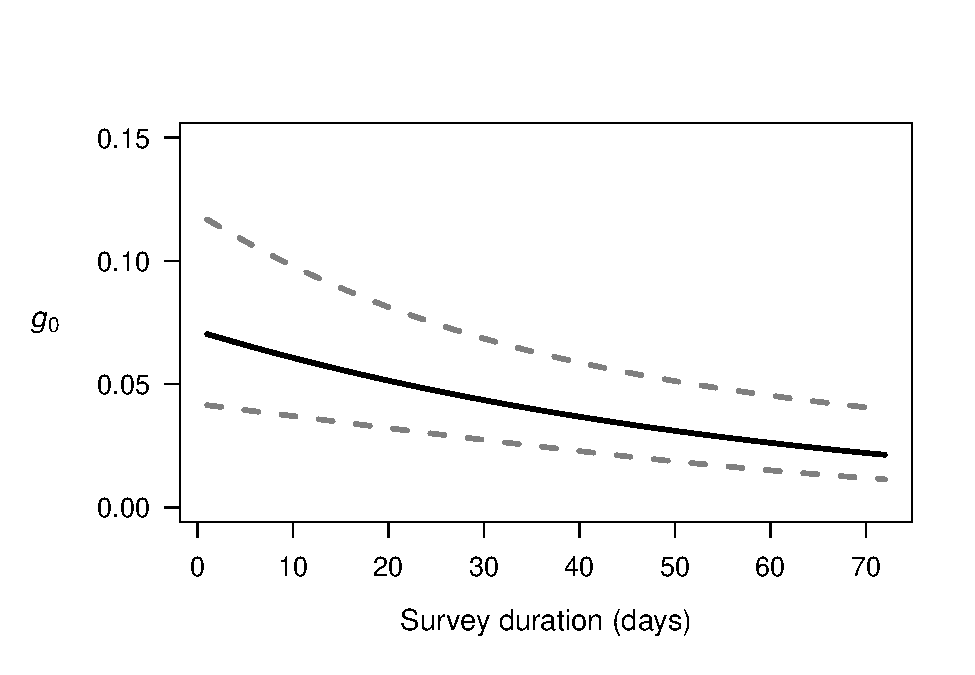
\includegraphics[width=0.7\linewidth]{figure/otways17-g0t-1} 

}

\caption{The AICc-best model linear trend in \textit{g}0 values (probability of daily detection in activity centre) throughout the survey. Grey dashed lines indicate 95\% confidence intervals.}\label{fig:otways17-g0t}
\end{figure}
\newpage

\(~\)

\(~\)

\(~\)

\begingroup\fontsize{10}{12}\selectfont
\begin{longtable}[t]{lrrrrrrr}
\caption{\label{tab:otways17-detfn}Model selection table and density estimates for different detection function shapes for spatial mark-resight models.}\\
\toprule
\multicolumn{5}{c}{Model comparison} & \multicolumn{3}{c}{Density estimate (cats km-2)} \\
\cmidrule(l{3pt}r{3pt}){1-5} \cmidrule(l{3pt}r{3pt}){6-8}
Detector function & K & AICc & dAICc & AICcwt & estimate & lcl & ucl\\
\midrule
\endfirsthead
\caption[]{\label{tab:otways17-detfn}Model selection table and density estimates for different detection function shapes for spatial mark-resight models. \textit{(continued)}}\\
\toprule
\multicolumn{5}{c}{Model comparison} & \multicolumn{3}{c}{Density estimate (cats km-2)} \\
\cmidrule(l{3pt}r{3pt}){1-5} \cmidrule(l{3pt}r{3pt}){6-8}
Detector function & K & AICc & dAICc & AICcwt & estimate & lcl & ucl\\
\midrule
\endhead

\endfoot
\bottomrule
\multicolumn{8}{l}{\rule{0pt}{1em}K - number of parameters}\\
\multicolumn{8}{l}{\rule{0pt}{1em}AICc - Akaike's Information Criterion with small-sample adjustment}\\
\multicolumn{8}{l}{\rule{0pt}{1em}dAICc - difference between AICc of this model and the model with smallest AICc}\\
\multicolumn{8}{l}{\rule{0pt}{1em}AICcwt - AICc model weight}\\
\multicolumn{8}{l}{\rule{0pt}{1em}lcl – lower 95\% confidence limit}\\
\multicolumn{8}{l}{\rule{0pt}{1em}ucl – upper 95\% confidence limit}\\
\endlastfoot
hazard-rate & 4 & 2359.59 & 0.00 & 0.7 & 1.15 & 0.93 & 1.42\\
exponential & 3 & 2361.25 & 1.66 & 0.3 & 1.19 & 0.96 & 1.49\\
halfnormal & 3 & 2373.30 & 13.72 & 0.0 & 1.12 & 0.93 & 1.35\\*
\end{longtable}
\endgroup{}

\hypertarget{occ-app}{%
\chapter{Supporting Information: Chapter \ref{occ}}\label{occ-app}}

\newpage

\begingroup\fontsize{10}{12}\selectfont
\begin{longtable}[t]{llrrrrrr}
\caption{\label{tab:occ-naive}Number of camera-trap sites, total deployments and naive occupancy rates for red foxes, feral cats, southern brown bandicoots (SBB) and long-nosed potoroos (LNP) within Ecological Vegetation Class groups across two broad regions in south-west Victoria, Australia.}\\
\toprule
Vegetation & Region & Sites & Deployments & Fox & Cat & SBB & LNP\\
\midrule
Dry Forest & Glenelg & 25 & 69 & 0.65 & 0.10 & 0.06 & 0.01\\
 & Otway & 111 & 314 & 0.42 & 0.28 & 0.02 & 0.06\\
Heathland & Glenelg & 40 & 119 & 0.43 & 0.34 & 0.14 & 0.18\\
 & Otway & 3 & 9 & 0.22 & 0.44 & 0.11 & 0.33\\
Heathy Woodland & Glenelg & 154 & 424 & 0.31 & 0.14 & 0.29 & 0.19\\
\addlinespace
 & Otway & 82 & 255 & 0.29 & 0.15 & 0.15 & 0.12\\
Herb-rich Woodland & Glenelg & 59 & 373 & 0.50 & 0.27 & 0.02 & 0.12\\
 & Otway & 2 & 6 & 0.33 & 0.17 & 0.00 & 0.00\\
Lowland Forest & Glenelg & 383 & 1046 & 0.46 & 0.18 & 0.17 & 0.05\\
 & Otway & 52 & 163 & 0.42 & 0.14 & 0.04 & 0.10\\
\addlinespace
Swampy Scrub & Glenelg & 4 & 10 & 0.60 & 0.50 & 0.00 & 0.00\\
 & Otway & 36 & 98 & 0.32 & 0.33 & 0.08 & 0.09\\
Wet Forest & Otway & 281 & 780 & 0.31 & 0.54 & 0.01 & 0.07\\
\bottomrule
\end{longtable}
\endgroup{}

\newpage
\begin{figure}

{\centering 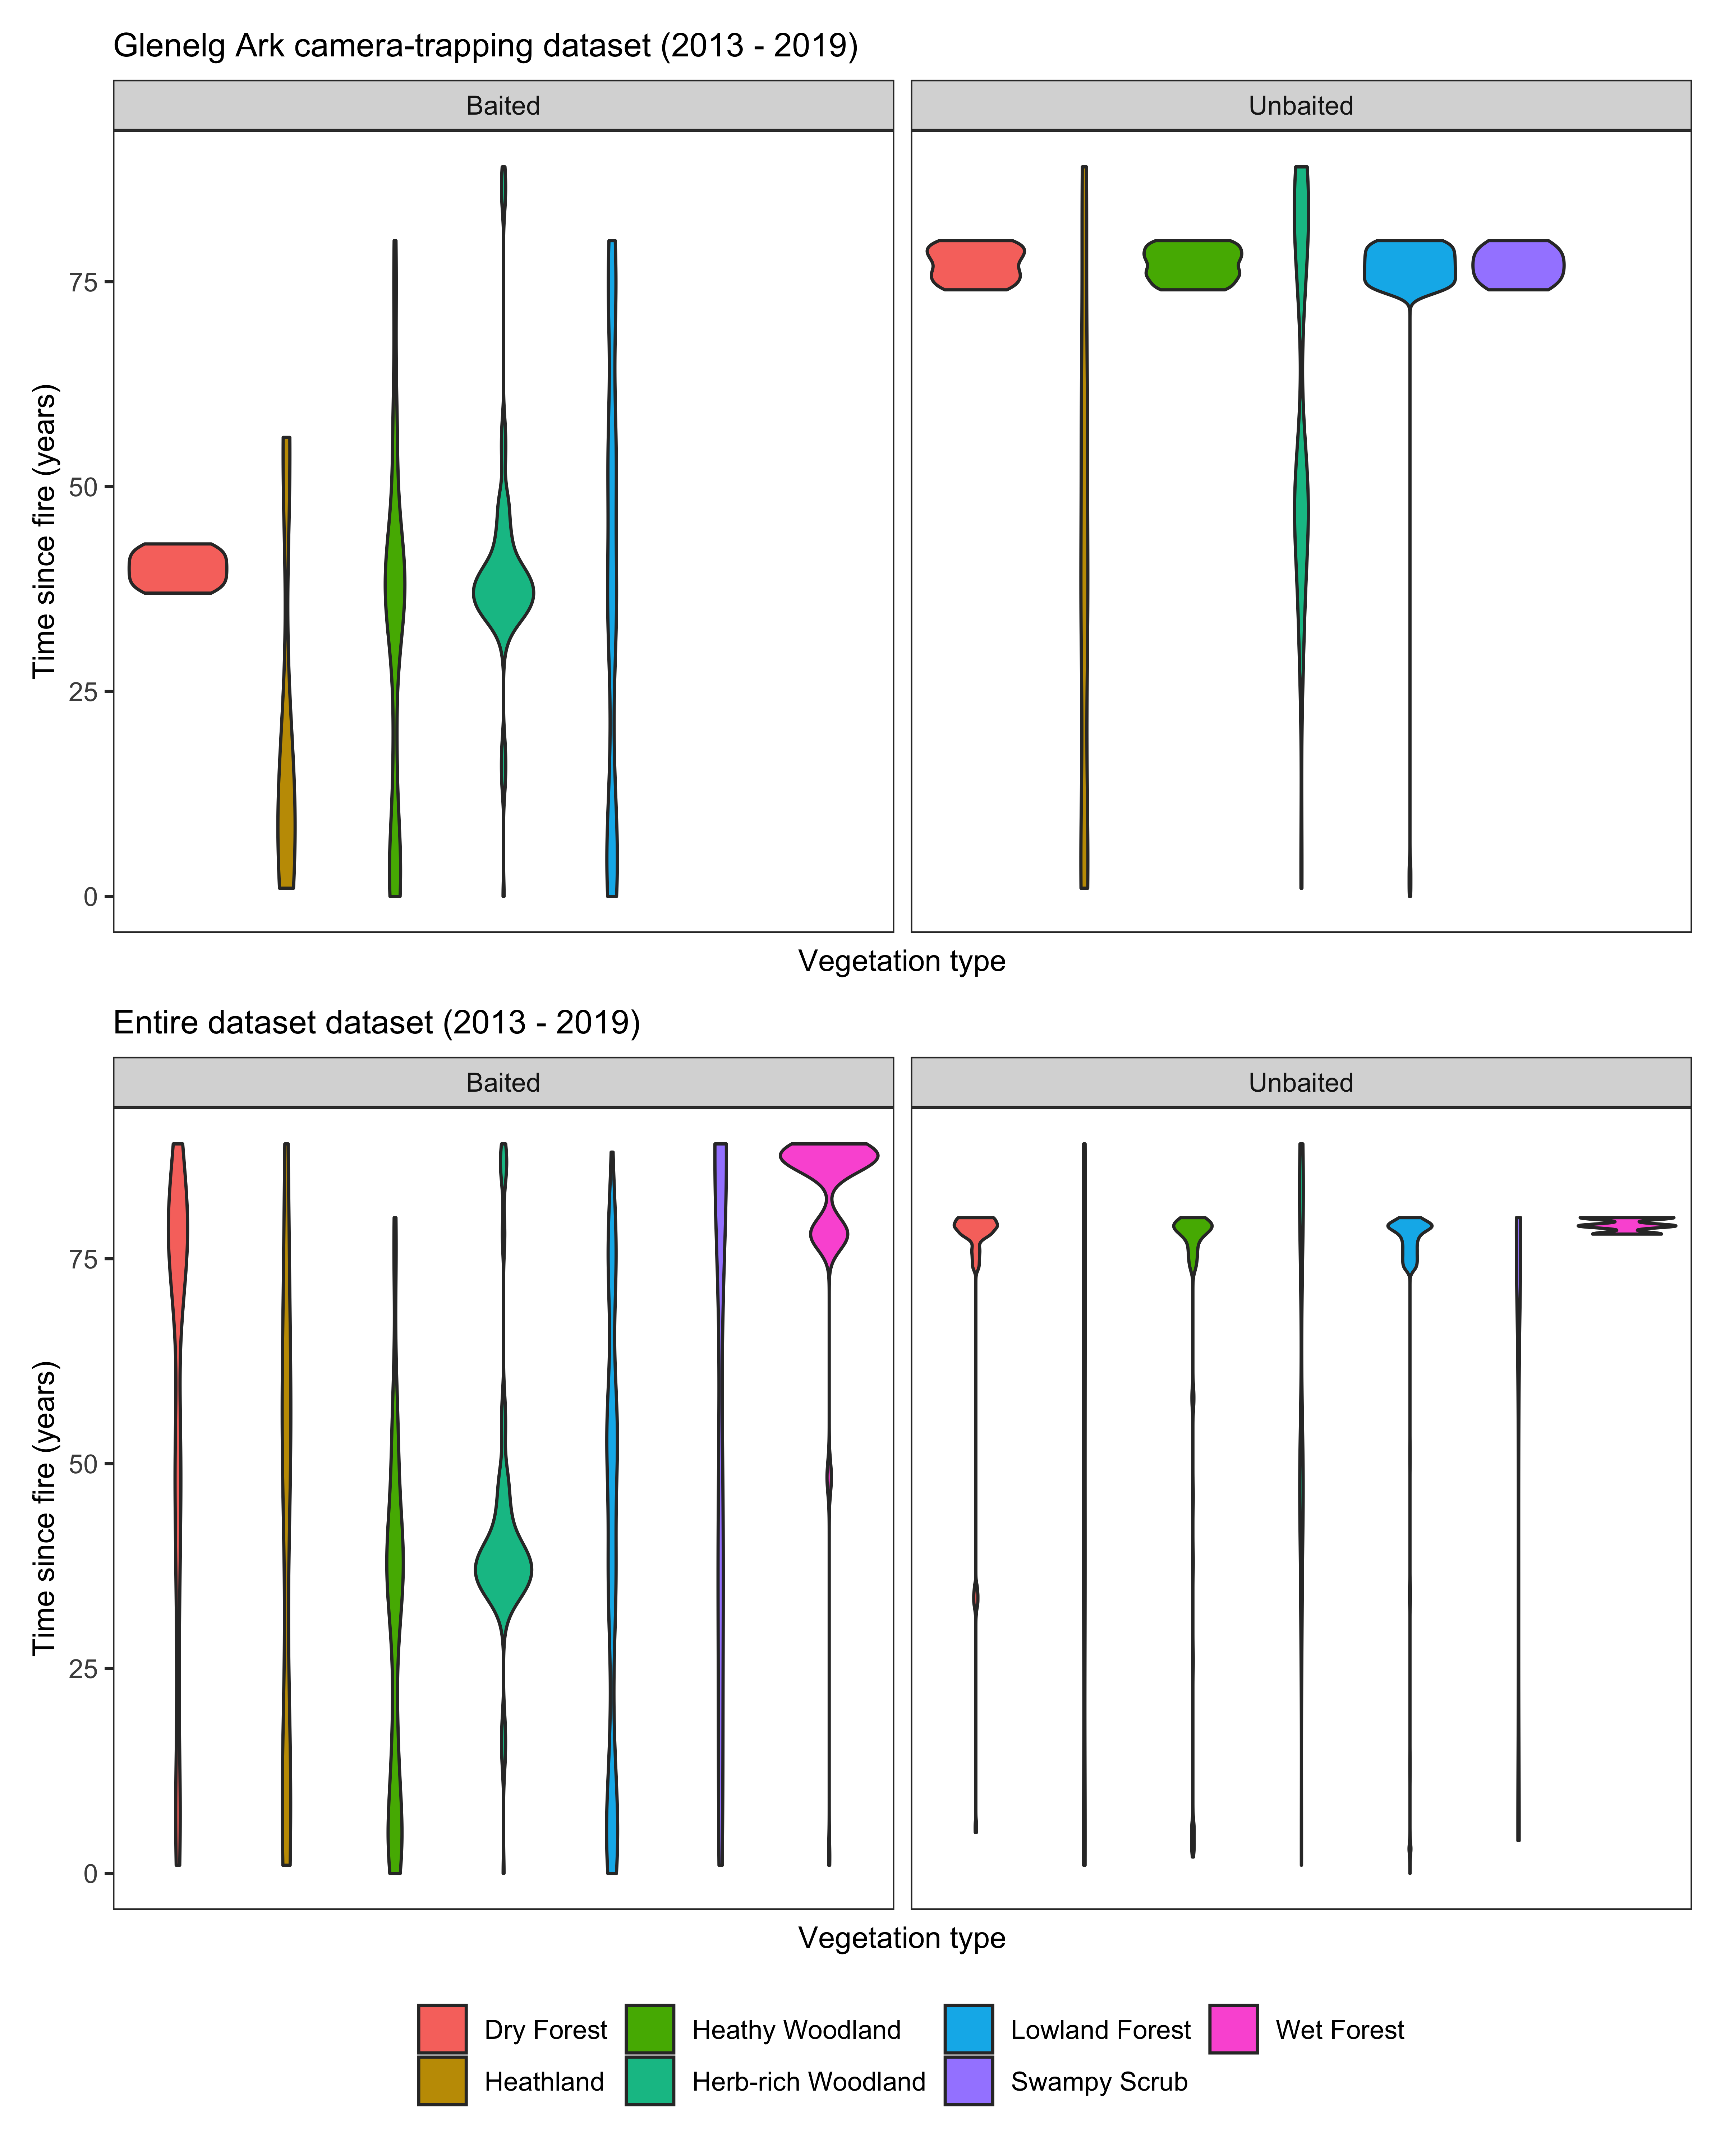
\includegraphics[width=1\linewidth]{figure/raw_data_tsf_veg} 

}

\caption{Range and distribution of time since fire values across the surveyed vegetation types in baited and unbaited sites. In the Glenelg Ark camera-trapping dataset, where most sites in the baited landscapes are relatively recently burnt, and most sites are long-unburnt in the unbaited landscapes. Combining M.W.R PhD and Otway Ark surveys provides a wider range of fire history patterns in each vegetation type with and without fox control.}\label{fig:veg-tsf-violin}
\end{figure}
\newpage
\begin{figure}

{\centering 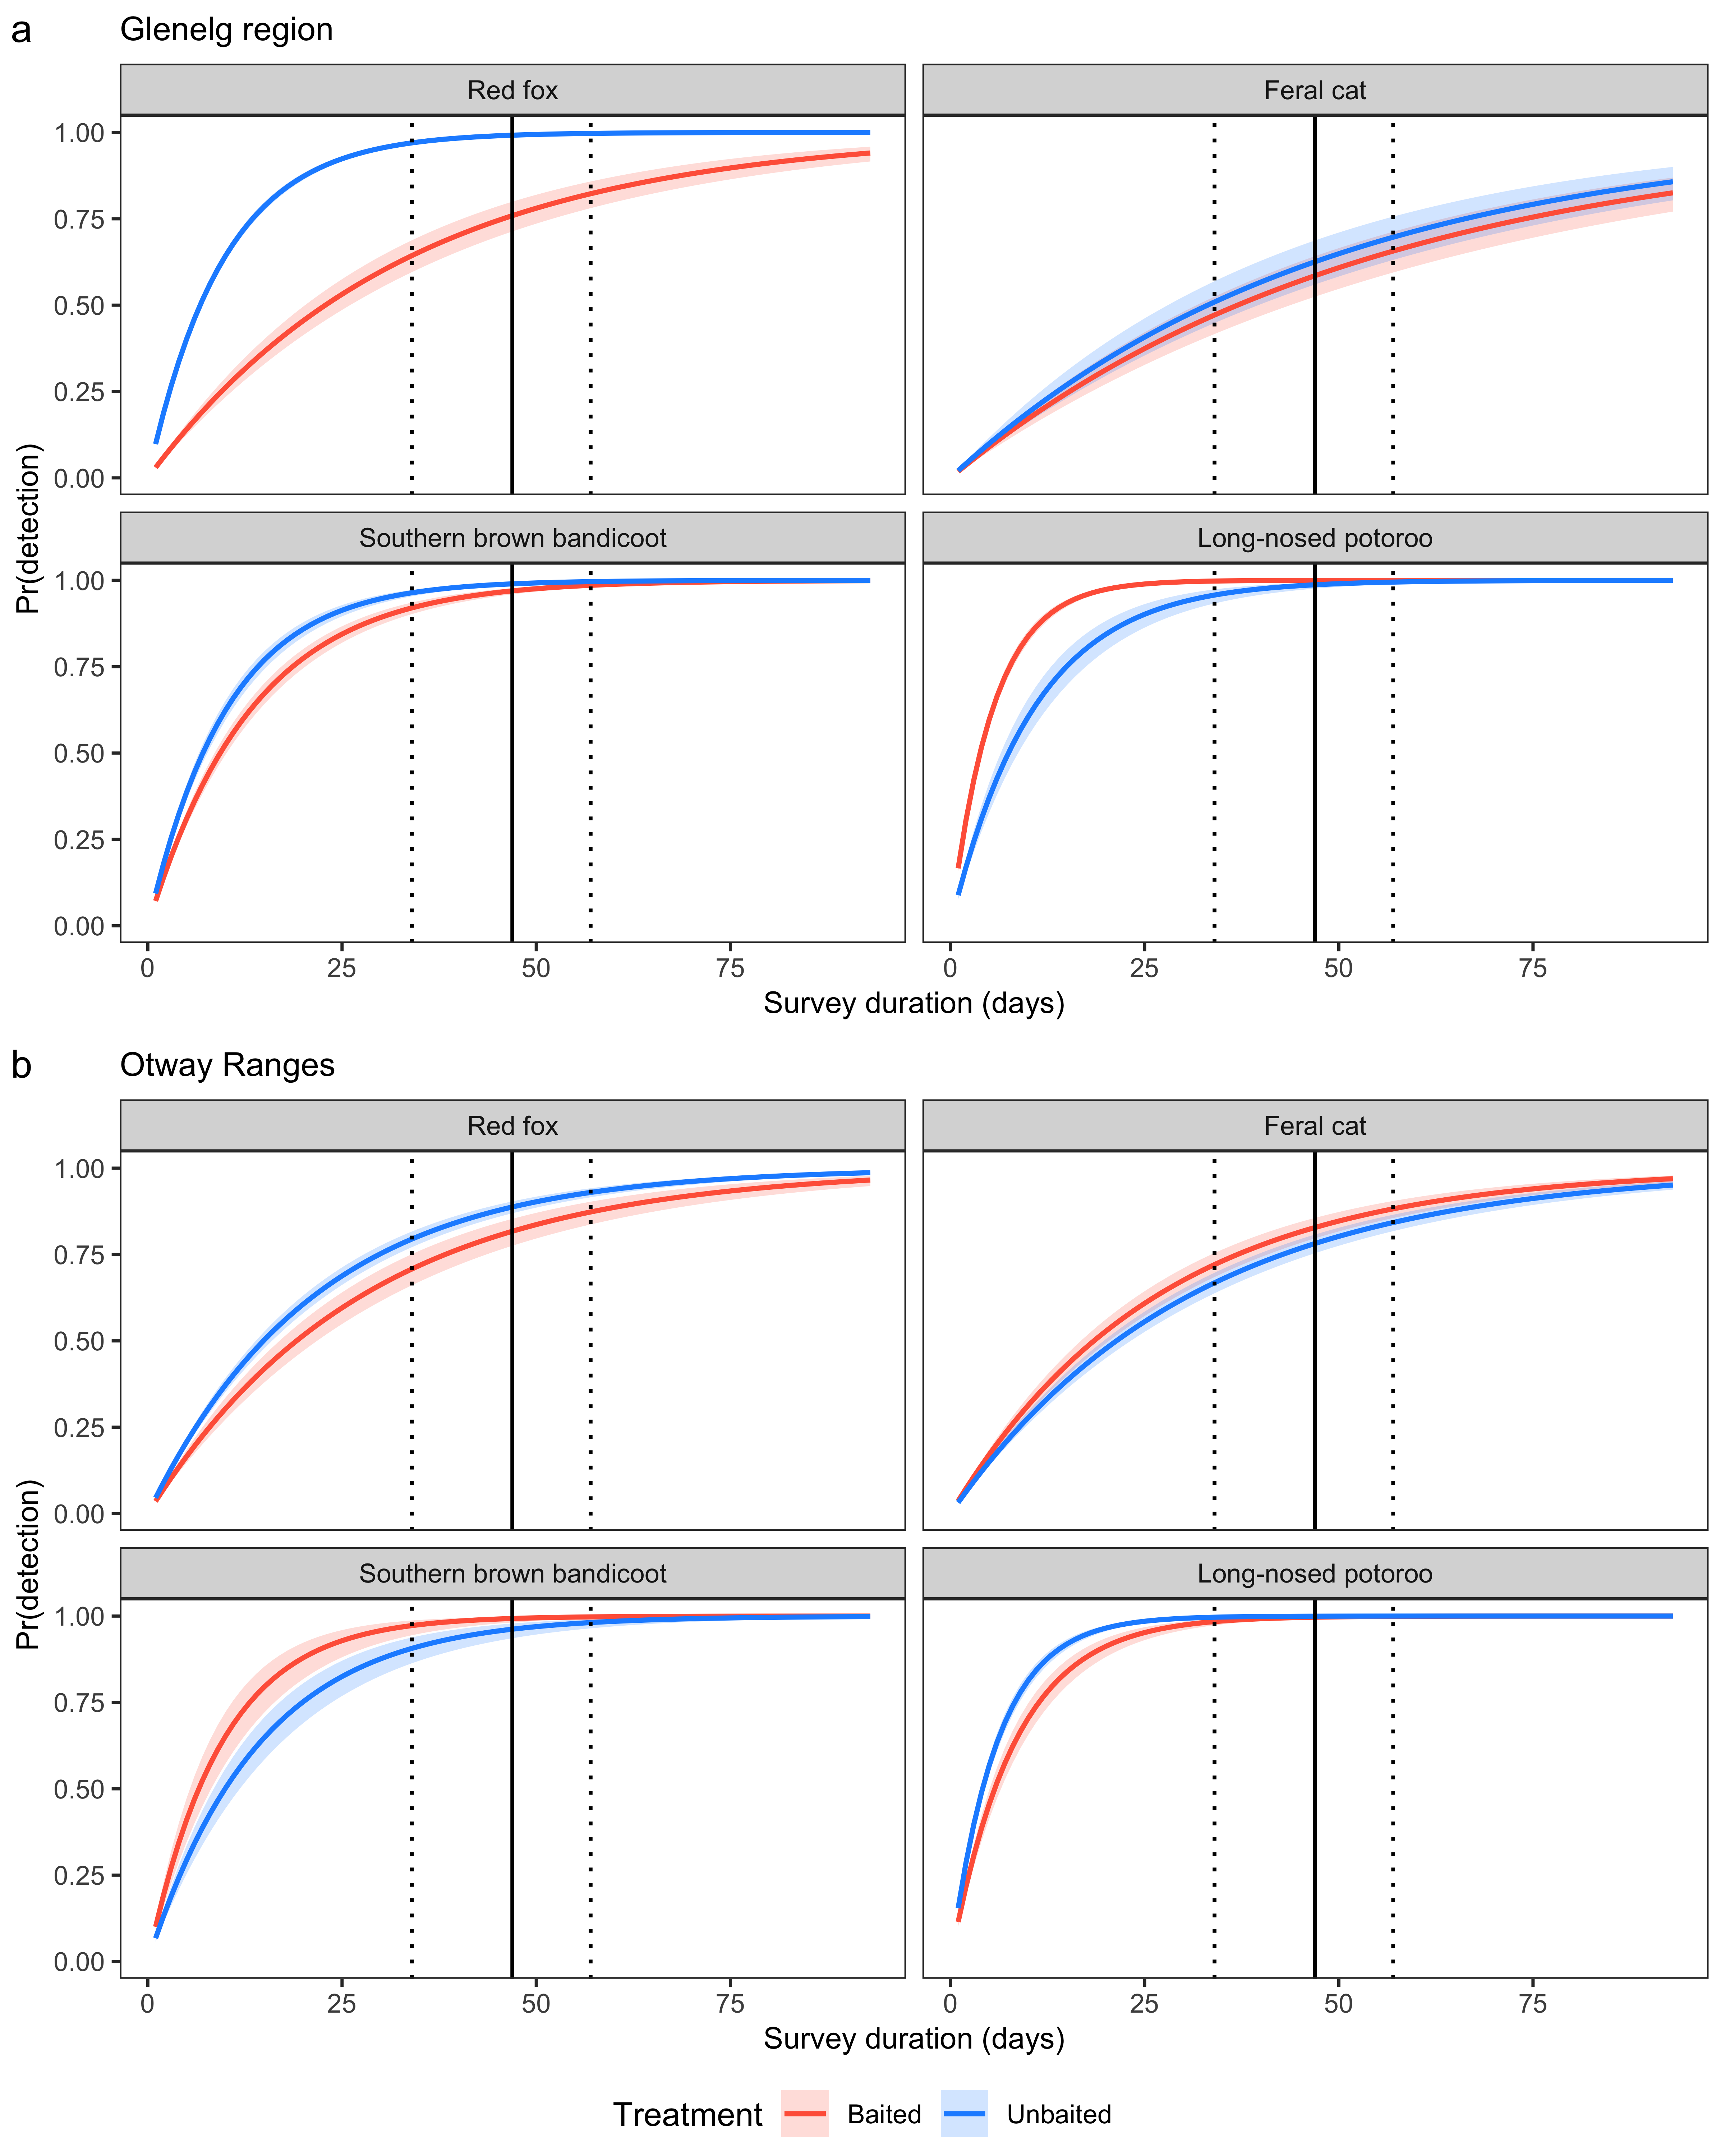
\includegraphics[width=1\linewidth]{figure/cumulative_detectability} 

}

\caption{Cumulative detection probabilities of species in landscapes with fox control (red) and without fox control (blue) in the Glenelg region (a) and Otway Ranges, south-west Victoria, Australia. Fox control had occurred in The Glenelg region for 8 - 13 years and was monitored with a control-impact design. The Otway Ranges was monitored using a before-after-control-impact experimental design; surveyed approximately 1 year prior and 2 years following the commencement of fox-baiting. Vertical grey lines represent mean (solid) as well as 25\% and 75\% quantiles (dotted) of days camera-traps were active for. Shaded bands represent 95\% Bayesian credible intervals. Estimates derived from Bayesian occupancy-detection models.}\label{fig:occ-cumdet}
\end{figure}
\newpage

\begingroup\fontsize{10}{12}\selectfont
\begin{longtable}[t]{lrrr}
\caption{\label{tab:occ-rain-aic}Akaike's Information Criterion values for generalised additive models with different rainfall periods.}\\
\toprule
Species & Months & AIC & dAIC\\
\midrule
Red fox & 6 & 4150.14 & 0.00\\
Red fox & 18 & 4151.57 & 1.43\\
Red fox & 24 & 4156.49 & 6.35\\
Red fox & 12 & 4158.20 & 8.06\\
Feral cat & 6 & 3732.68 & 0.00\\
\addlinespace
Feral cat & 12 & 3733.39 & 0.71\\
Feral cat & 18 & 3733.39 & 0.71\\
Feral cat & 24 & 3733.39 & 0.71\\
Southern brown bandicoot & 6 & 1868.55 & 0.00\\
Southern brown bandicoot & 24 & 1868.56 & 0.00\\
\addlinespace
Southern brown bandicoot & 18 & 1874.10 & 5.54\\
Southern brown bandicoot & 12 & 1877.49 & 8.94\\
Long-nosed potoroo & 12 & 1577.71 & 0.00\\
Long-nosed potoroo & 18 & 1581.19 & 3.48\\
Long-nosed potoroo & 24 & 1581.34 & 3.62\\
\addlinespace
Long-nosed potoroo & 6 & 1582.96 & 5.25\\
\bottomrule
\multicolumn{4}{l}{\rule{0pt}{1em}\textit{Note: }}\\
\multicolumn{4}{l}{\rule{0pt}{1em}AIC - Akaike's Information Criterion score}\\
\multicolumn{4}{l}{\rule{0pt}{1em}dAIC - difference between AIC of this model and the model with smallest AIC}\\
\end{longtable}
\endgroup{}

\newpage
\begin{figure}

{\centering 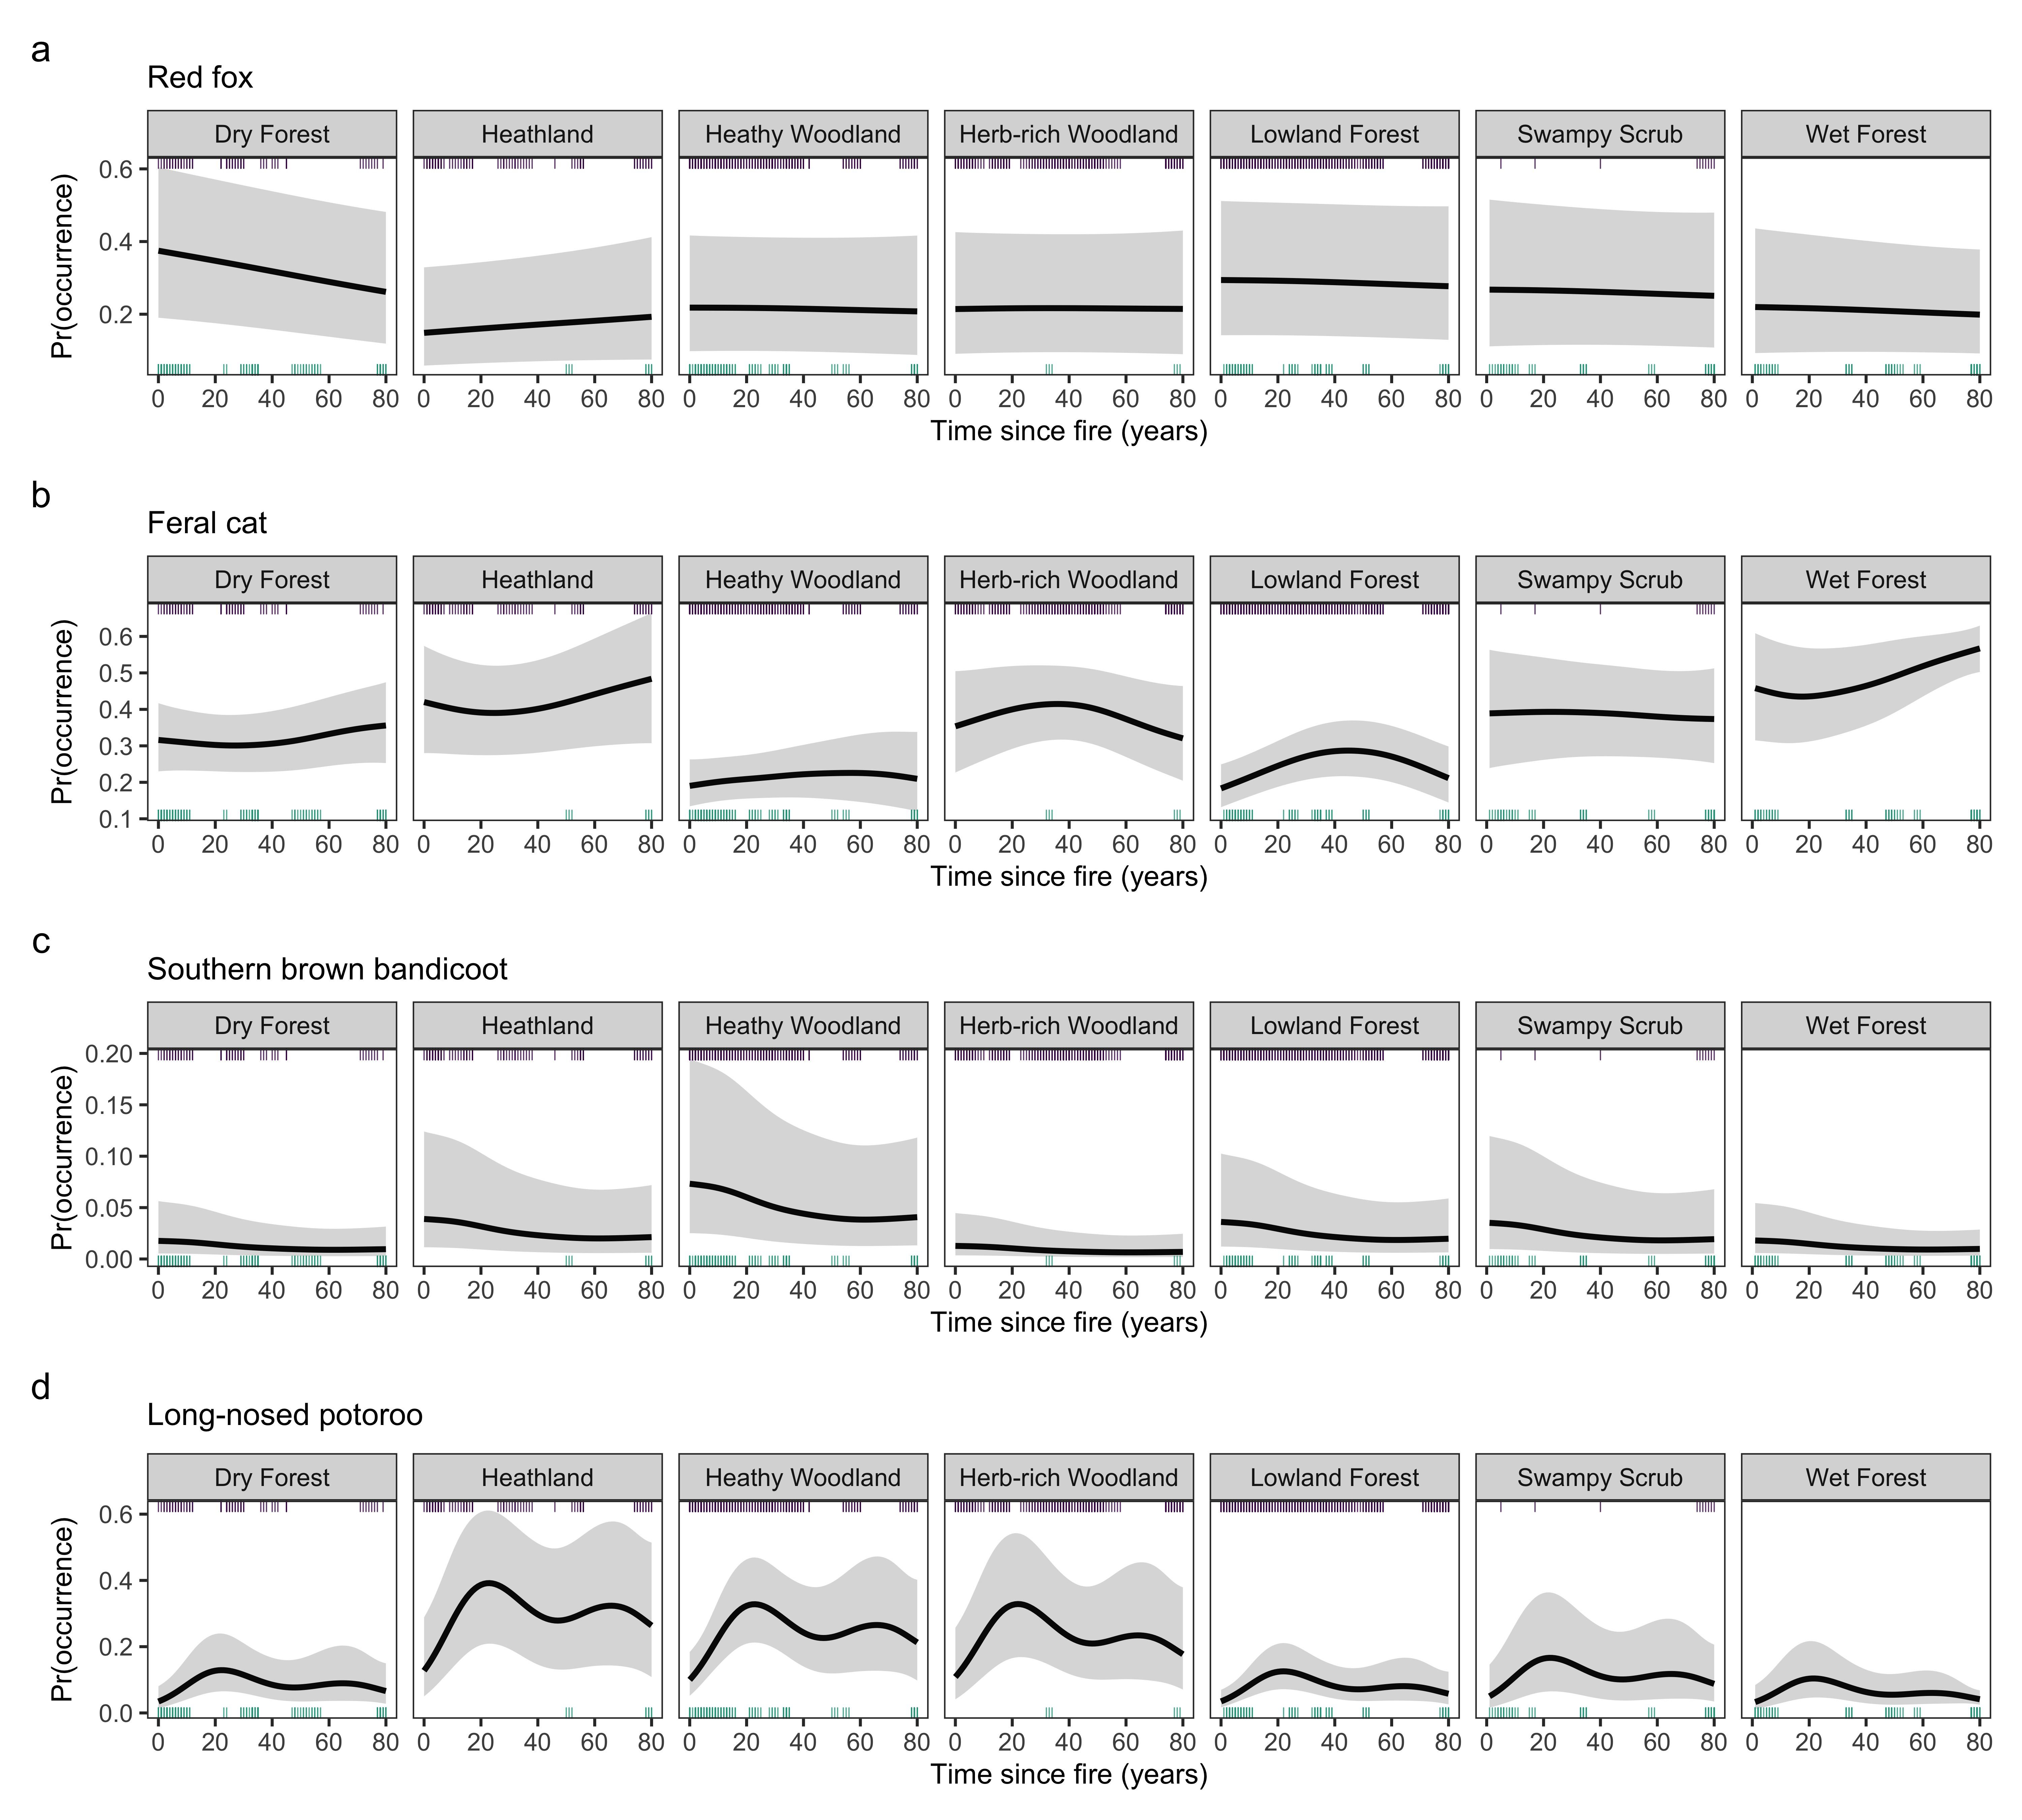
\includegraphics[width=1\linewidth]{figure/tsf} 

}

\caption{Time since fire had a weak impact on fox (a) and feral cat (b) occupancy probability in south-west Victoria, Australia. Southern brown bandicoot occupancy probability (c) peaked around 15 and 75 years following fire, although, the magnitude of both peaks differed across Ecological Vegetation Class groups. Long-nosed potoroo occupancy probability (d) linearly increased with time since fire in heathy vegetation groups, but linearly decreased with years post-fire in Herb-Rich Woodlands. Estimates derived from generalised additive models (assuming perfect detection). Shaded regions indicate 95\% confidence intervals. Rug ticks representing the distribution of time since fire data for the Glenelg region (brown) is shown on the inside of the top axis, Otway Ranges distribution shown on the inside of the bottom axis (navy).}\label{fig:occ-tsf}
\end{figure}
\hypertarget{density-app}{%
\chapter{Supporting Information: Chapter \ref{density}}\label{density-app}}

\newpage

\hypertarget{density-app-field}{%
\section{Field surveys}\label{density-app-field}}

In the Glenelg region, we deployed camera-traps once at a unique sites once. In the Otway region, we redeployed camera-traps in sites three times annually. All 2017 camera-sites were resurveyed each year, except for four logistically challenging sites in the southern grid. In 2018, we added 16 additional sites in the southern grid, as well as 36 additional sites in the northern grid. These additional sites were resurveyed in 2019.

At each site, we deployed a singular remote trail camera with infrared flash and temperature-in-motion detector. The vast majority of camera-traps were Reconyx Hyperfire HC600, but a small portion was made up of both PC900 and HF2X infrared models (Reconyx, Holmen, Wisconsin). We programmed camera's to the highest sensitivity and to take five consecutive photographs when triggered (no quiet period). We attached each camera to a tree, approximately 30 cm above the ground, and facing toward a lure 2 - 2.5 metres away. The lure comprised an oil-absorbing cloth doused in tuna oil and placed inside a PVC pipe container with a mesh top. We secured each lure to the top of a 1 metre wooden stake and attached a handful of small white feathers to the outside of the PVC pipe container. Feathers were not used in the Lower Glenelg National Park survey. We cleared vegetation in the camera's line-of-sight to reduce false triggers and avoid obscuring cat coat markings in images.

\newpage

\(~\)

\(~\)

\(~\)
\begin{figure}

{\centering 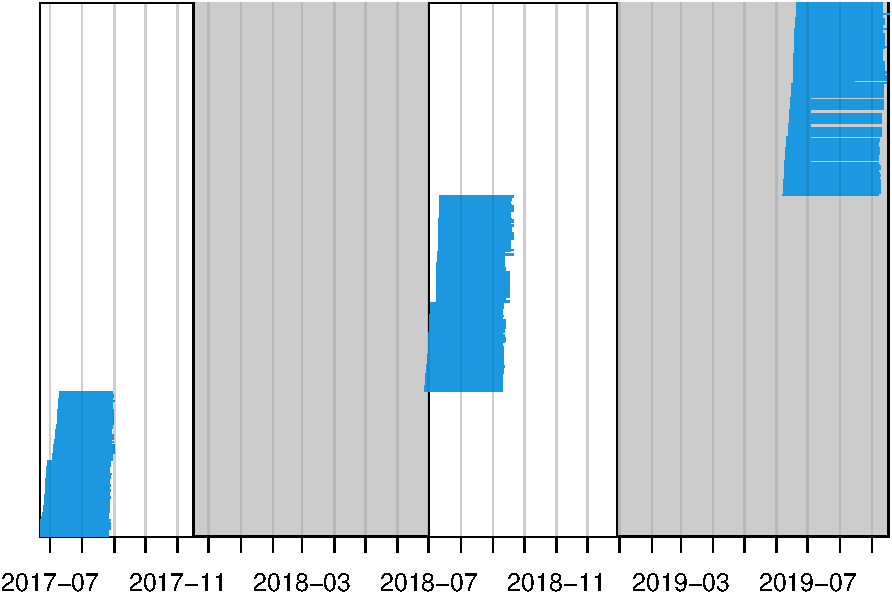
\includegraphics[width=1\linewidth]{figure/density-camop-1} 

}

\caption{Camera-trap operation times in the Otway region, Australia. Each blue horizontal line represents one camera-trap deployment. Grey shading indicates periods of fox control in the impact landscape.}\label{fig:density-camop}
\end{figure}
\newpage

\(~\)

\(~\)

\(~\)
\begin{figure}

{\centering 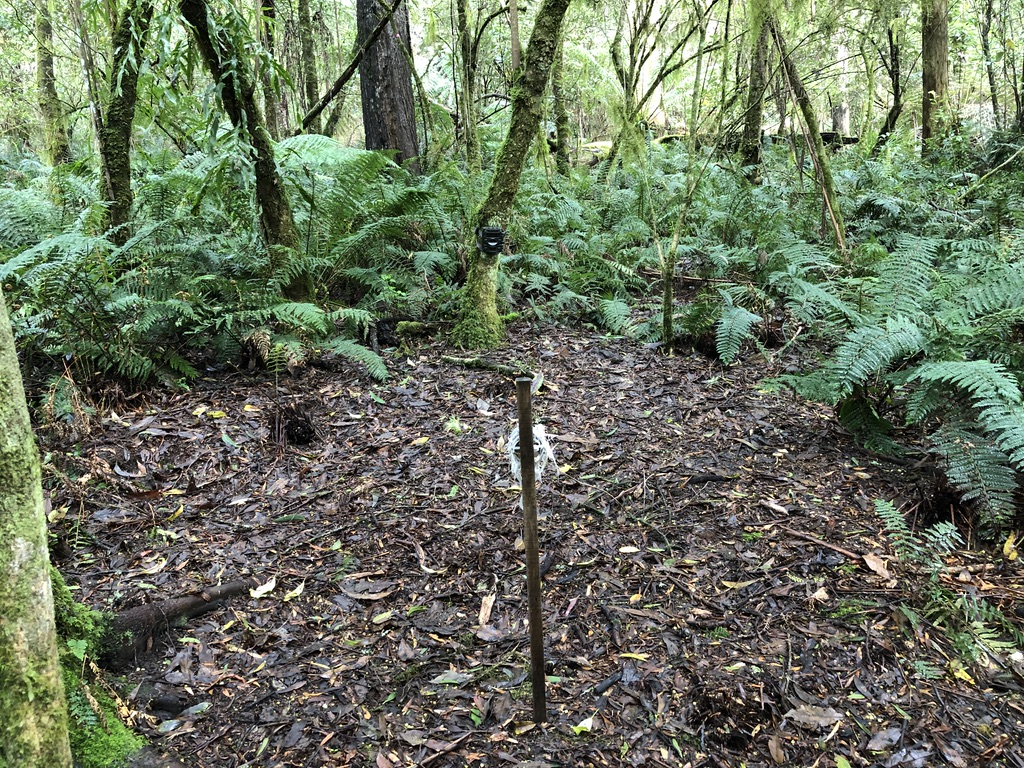
\includegraphics[width=1\linewidth]{figure/camtrap1} 

}

\caption{Example of a typical camera-trap set-up in the Otway region, Australia.}\label{fig:density-cam-photo}
\end{figure}
\newpage

\hypertarget{density-app-id}{%
\section{Individual cat identification}\label{density-app-id}}

We first labelled every camera-trap image with a species metadata tag using \href{https://www.digikam.org}{DigiKam software}. We also added metadata tags for each cat coat type: black, mackerel tabby, classic tabby, ginger and other (coats with multiple colour blends; Fig. 3). This allowed us to summarise species records and extract cat images using the `camtrapR' R-package (Niedballa \emph{et al.} 2016).

We considered all black cats to be of the `unmarked' category in spatial mark-resight models - even the few with white splotches on their underside (as these couldn't always be seen as cats move with their head down).

In the remaining coat categories where possible, we identified individual cats based on their unique coat markings. The ability to identify individuals substantially increased as the image library for each cat increased. Therefore we made the easiest identifications first to build up these libraries, before making decisions on the less obvious detections. We examined and matched all coat markings seen between two particular defections. Markings on the front legs were the most useful for ID's as the patterns do not skew as much with different body positions. On the whole, unidentifiable detections were mainly due to only part of a cat appearing in the frame, or because photos were blurry (because of cat movement or a foggy camera lens).

We were left with a small number of instances (less than ten) where only left or right flanks could be seen. In this case, the side with the most repeat detections was labelled as an individual, whereas the side with the least number of detections was considered unidentifiable. Additionally, an extremely small portion of cats in the Otways had ginger coats. When ginger coats are photographed with an infrared flash, they become overexposed and no markings can be seen (see the image in bottom-right corner in Fig. S3). We only had one detection of a ginger cat without an infrared coat. Therefore, if there were multiple ginger cat detections in a single grid, we treated them in the same way as one-sided flank detections.

One observer identified the 2018 feral cats in the Glenelg region (MR) and the 2021 Lower Glenelg National Park cats (Luke Woodford). In the 2017 and 2018 Otway datasets (where there were substantially more cat detections and fewer distinct coat patterns) two independent observers identified individual cats and discrepancies between observers were reviewed together until consensus was reached (MR, MLP, BH). If no consensus was reached, the cat was considered unidentifiable. In the 2019 Otway dataset, many of the identified cats were sighted in the previous surveys -- these larger individual libraries meant that cats could be identified more easily so only one observer was necessary (MR). We also made use of additional cat images taken within the Otway region grids (just before each of our surveys) by white flash camera-traps from another study (Zoï Banikos, unpublished data). This provided additional and higher quality images (due to the white flash) of individuals in the photo library for identifications.

We were therefore left with three groups of cats: unmarked (black cats), marked (cats which could be identified to the individual-level with complete certainty) and mark status unknown (cats which were not black, but couldn't be identified to the individual level with complete certainty).

We ignored the few detections of cats which were obviously young enough to be dependent on a parent, as these kittens do not have independent activity centres or movements and were not yet recruited into the adult population.

\newpage

\(~\)

\(~\)

\(~\)
\begin{figure}

{\centering 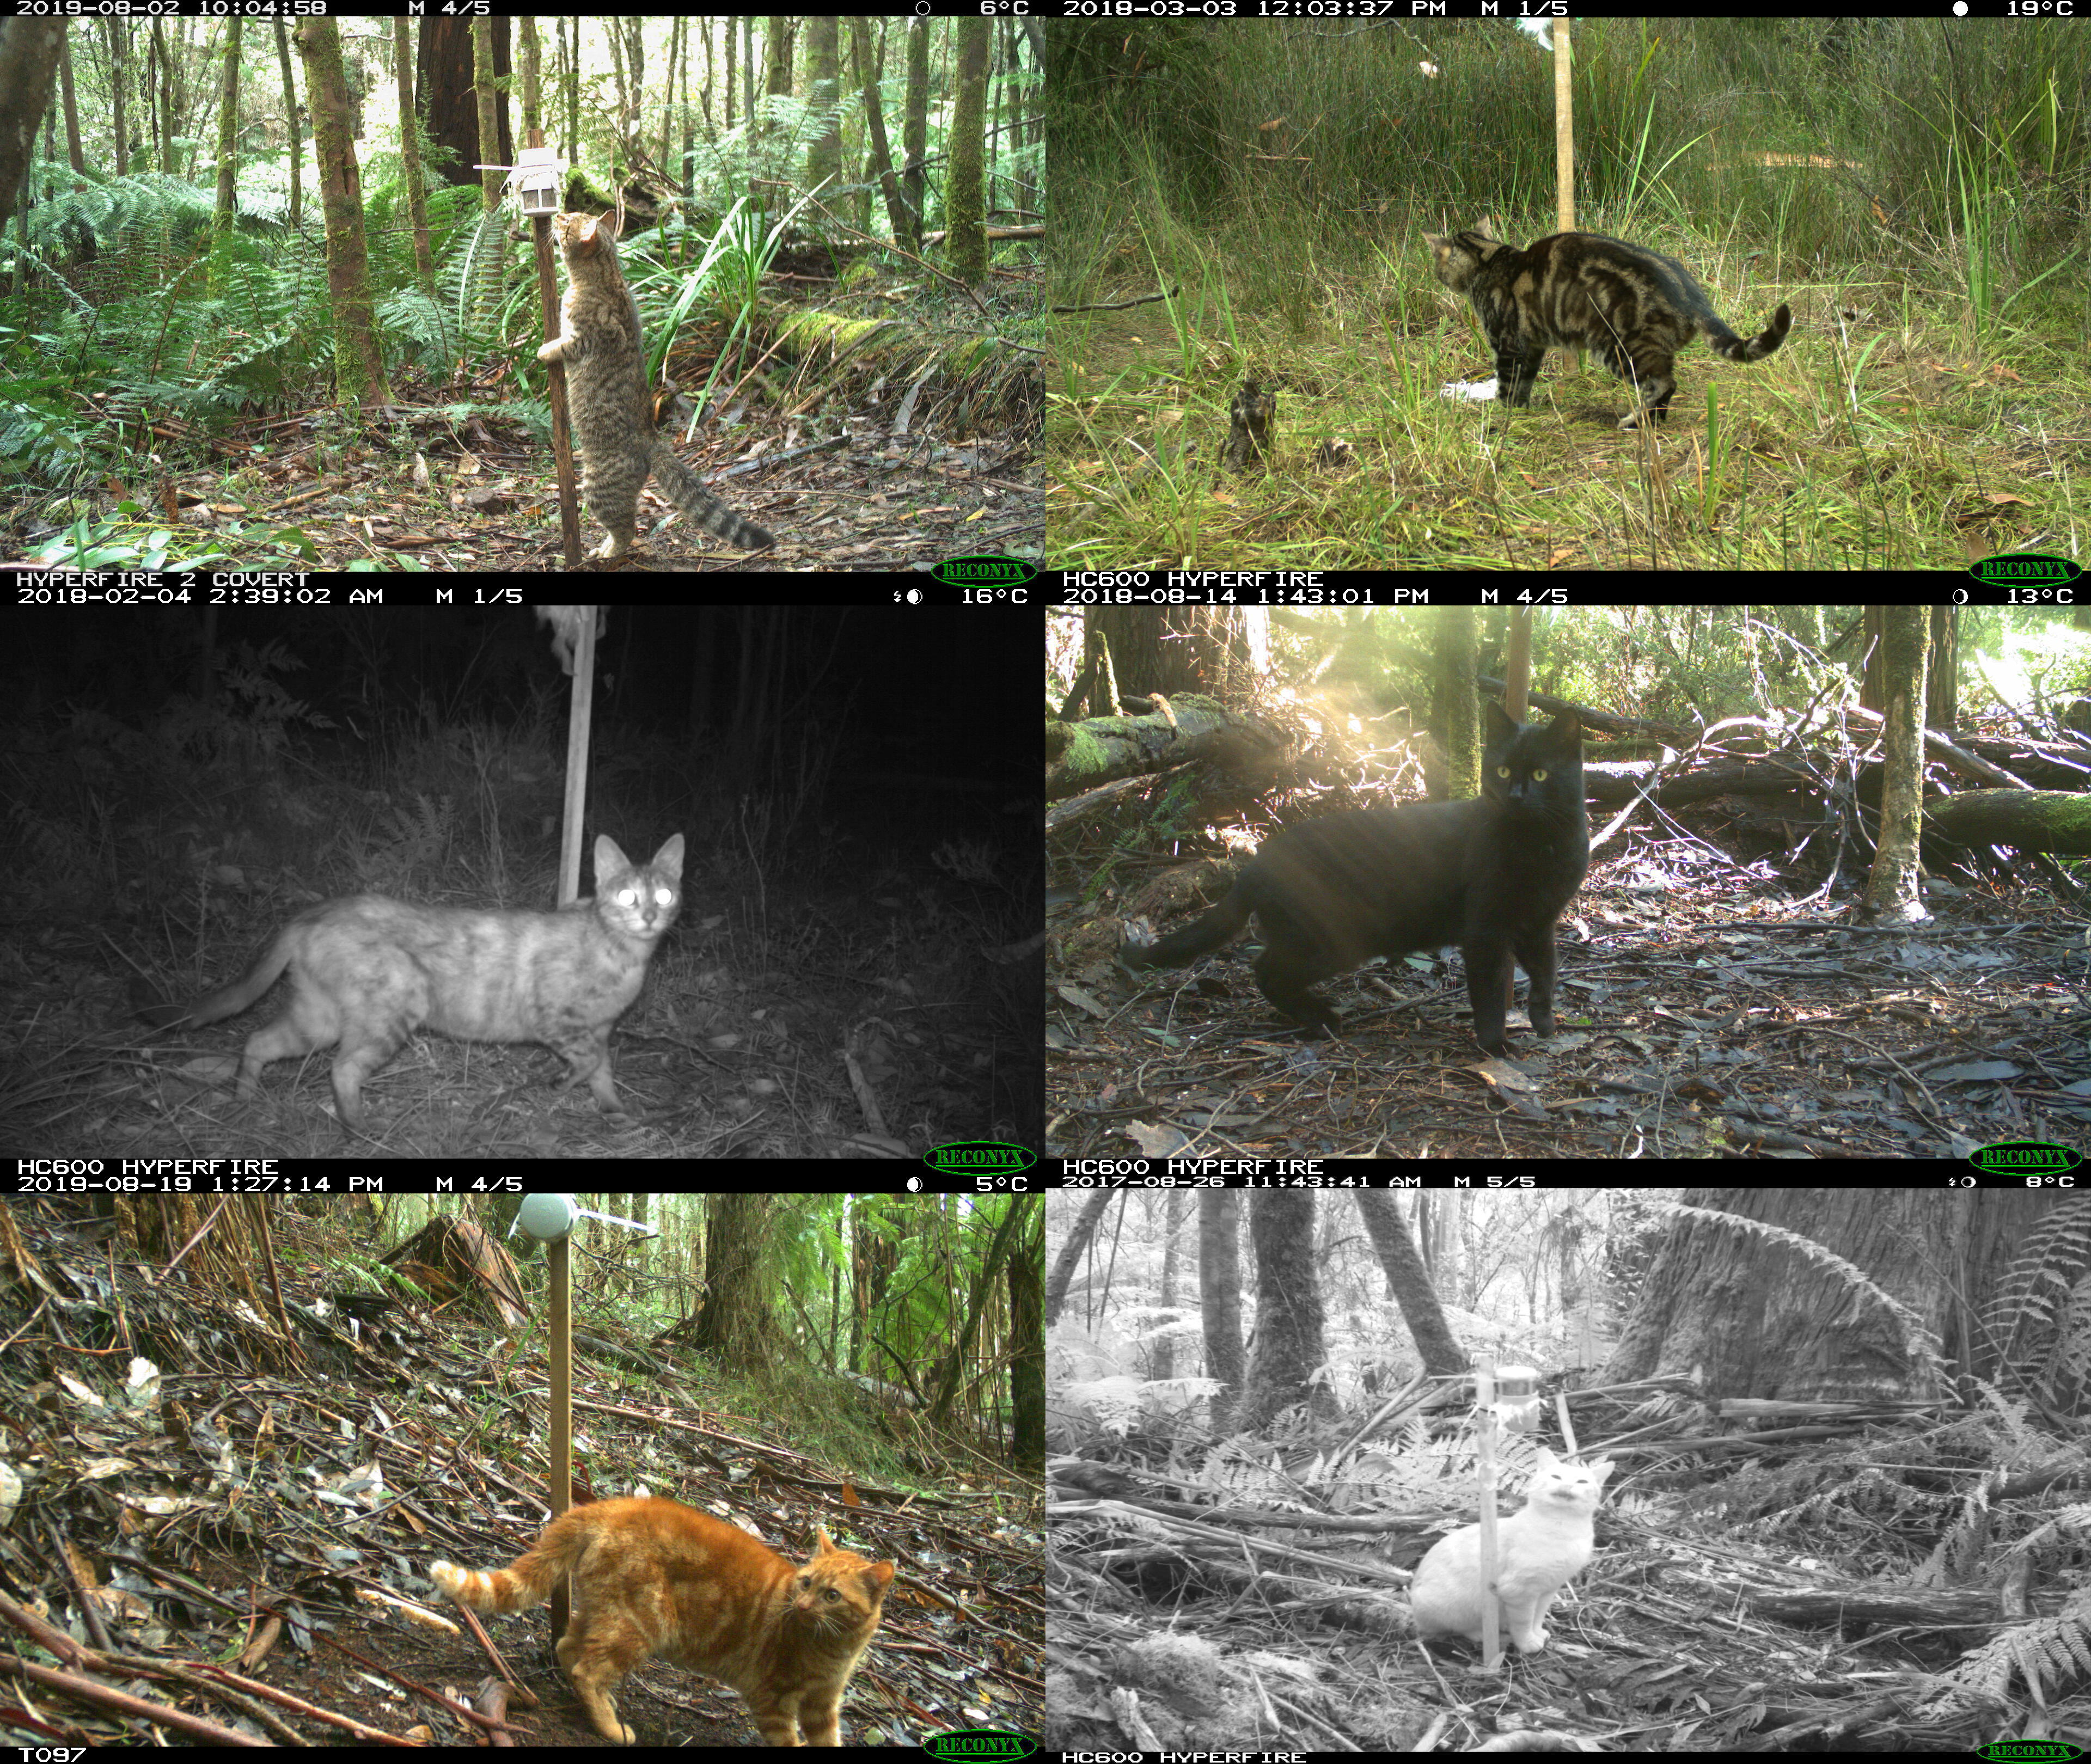
\includegraphics[width=1\linewidth]{figure/cat_coats} 

}

\caption{Feral cat coat categories from left-right, top-bottom: black, mackerel tabby, classic tabby, other, black, ginger and ginger with infrared flash.}\label{fig:density-cat-photo}
\end{figure}
\newpage

\hypertarget{summary-statistics}{%
\section{Summary statistics}\label{summary-statistics}}

\(~\)

\(~\)

\(~\)

\begingroup\fontsize{10}{12}\selectfont
\begin{longtable}[t]{lrrrrrrr}
\caption{\label{tab:density-stats}Summary of camera-trap survey effort and feral cat detections.}\\
\toprule
\multicolumn{5}{c}{ } & \multicolumn{3}{c}{Detections (max. 1 per 24-hr)} \\
\cmidrule(l{3pt}r{3pt}){6-8}
Landscape & Cameras & Trapnights & Cats & Moves & Identified & Unidentified & Unmarked\\
\midrule
\endfirsthead
\caption[]{\label{tab:density-stats}Summary of camera-trap survey effort and feral cat detections. \textit{(continued)}}\\
\toprule
\multicolumn{5}{c}{ } & \multicolumn{3}{c}{Detections (max. 1 per 24-hr)} \\
\cmidrule(l{3pt}r{3pt}){6-8}
Landscape & Cameras & Trapnights & Cats & Moves & Identified & Unidentified & Unmarked\\
\midrule
\endhead

\endfoot
\bottomrule
\endlastfoot
Annya & 110 & 8000 & 9 & 11 & 23 & 3 & 20\\
Cobbob & 110 & 7752 & 13 & 19 & 35 & 9 & 37\\
Hotspur & 99 & 6085 & 8 & 12 & 22 & 3 & 13\\
Mt Clay & 106 & 5451 & 10 & 16 & 33 & 5 & 0\\
LGNP north & 49 & 2102 & 6 & 3 & 11 & 0 & 0\\
\addlinespace
LGNP south & 64 & 2842 & 21 & 4 & 37 & 0 & 0\\
North 2017 & 67 & 3565 & 26 & 12 & 60 & 8 & 46\\
South 2017 & 73 & 7099 & 20 & 18 & 62 & 4 & 48\\
North 2018 & 103 & 7838 & 30 & 32 & 90 & 12 & 62\\
South 2018 & 85 & 4543 & 24 & 37 & 75 & 17 & 59\\
\addlinespace
North 2019 & 99 & 6077 & 27 & 39 & 90 & 22 & 101\\
South 2019 & 86 & 7150 & 25 & 69 & 133 & 23 & 58\\*
\end{longtable}
\endgroup{}

\newpage

\hypertarget{feral-cat-detection-plots}{%
\section{Feral cat detection plots}\label{feral-cat-detection-plots}}

\hypertarget{glenelg-region-3}{%
\subsection{Glenelg region}\label{glenelg-region-3}}

\hypertarget{replicate-1}{%
\subsubsection{Replicate 1}\label{replicate-1}}

\(~\)

\(~\)

\(~\)
\begin{figure}

{\centering 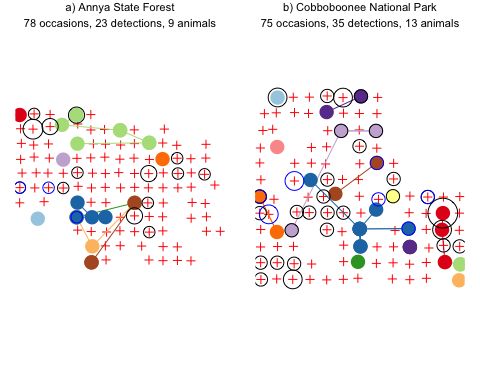
\includegraphics[width=1\linewidth]{figure/density-plot-ch-1-1} 

}

\caption{Feral cat detections in the first replicate grid pair in the Glenelg region, Australia. Camera-traps are indicated by red crosses. Solid fill coloured circles represent identified cats with lines indicating observed movements. Black open circles indicate black cat detections; blue circles indicate unidentifiable tabby cat detections, with circle radius scaling positively with the number of daily detections. Fox control does not occur in Annya (a) but does in Cobboboonee (b).}\label{fig:density-plot-ch-1}
\end{figure}
\newpage

\hypertarget{replicate-2}{%
\subsubsection{Replicate 2}\label{replicate-2}}

\(~\)

\(~\)

\(~\)
\begin{figure}

{\centering 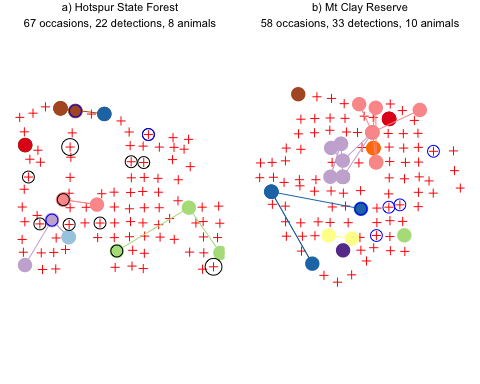
\includegraphics[width=1\linewidth]{figure/density-plot-ch-2-1} 

}

\caption{Feral cat detections in the second replicate grid pair in the Glenelg region, Australia. Camera-traps are indicated by red crosses. Solid fill coloured circles represent identified cats with lines indicating observed movements. Black open circles indicate black cat detections; blue circles indicate unidentifiable tabby cat detections, with circle radius scaling positively with the number of daily detections. Fox control does not occur in Hotspur (a) but does in Mt Clay (b).}\label{fig:density-plot-ch-2}
\end{figure}
\newpage

\hypertarget{replicate-3}{%
\subsubsection{Replicate 3}\label{replicate-3}}

\(~\)

\(~\)

\(~\)
\begin{figure}

{\centering 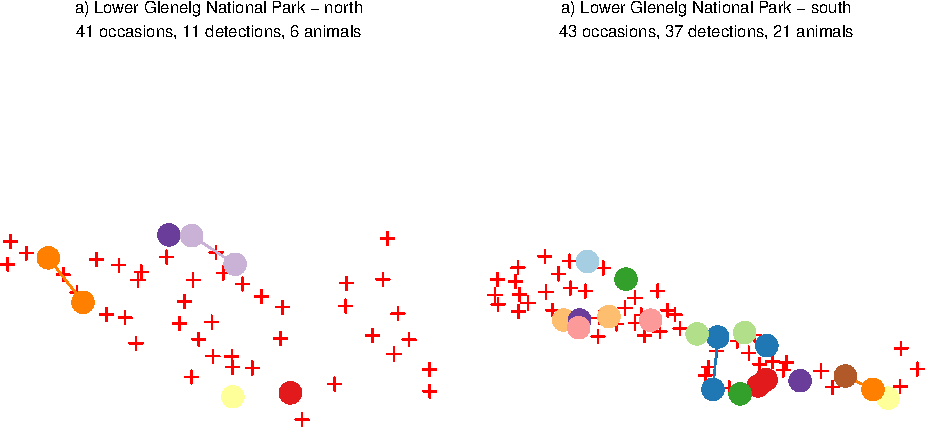
\includegraphics[width=1\linewidth]{figure/density-plot-ch-3-1} 

}

\caption{Feral cat detections in the third replicate grid pair in the Glenelg region, Australia. Camera-traps are indicated by red crosses. Solid fill coloured circles represent identified cats with lines indicating observed movements. Black open circles indicate black cat detections; blue circles indicate unidentifiable tabby cat detections, with circle radius scaling positively with the number of daily detections. Fox control does not occur in the north (a) but does in the south (b).}\label{fig:density-plot-ch-3}
\end{figure}
\newpage

\hypertarget{otway-region}{%
\subsection{Otway region}\label{otway-region}}

\hypertarget{section}{%
\subsubsection{2017}\label{section}}

\(~\)

\(~\)

\(~\)
\begin{figure}

{\centering 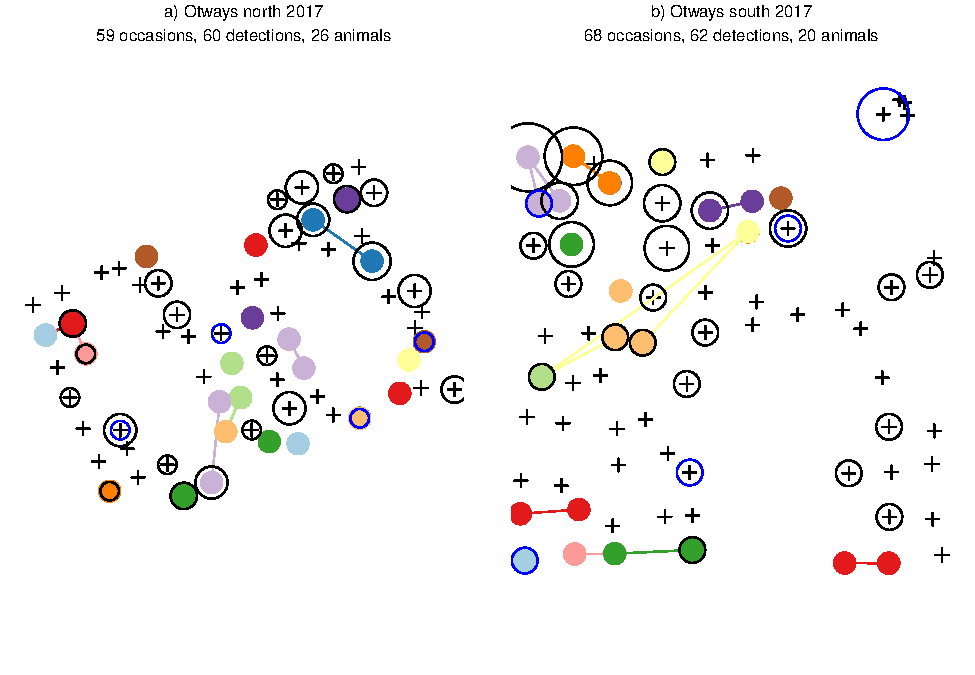
\includegraphics[width=1\linewidth]{figure/density-plot-ch-4-1} 

}

\caption{Feral cat detections in the Otway region, Australia, 2017. Solid fill coloured circles represent identified cats with lines indicating observed movements. Black open circles indicate black cat detections; blue circles indicate unidentifiable tabby cat detections, with circle radius scaling positively with the number of daily detections. Fox control did not occur in either of the landscapes during this time.}\label{fig:density-plot-ch-4}
\end{figure}
\newpage

\hypertarget{section-1}{%
\subsubsection{2018}\label{section-1}}

\(~\)

\(~\)

\(~\)
\begin{figure}

{\centering 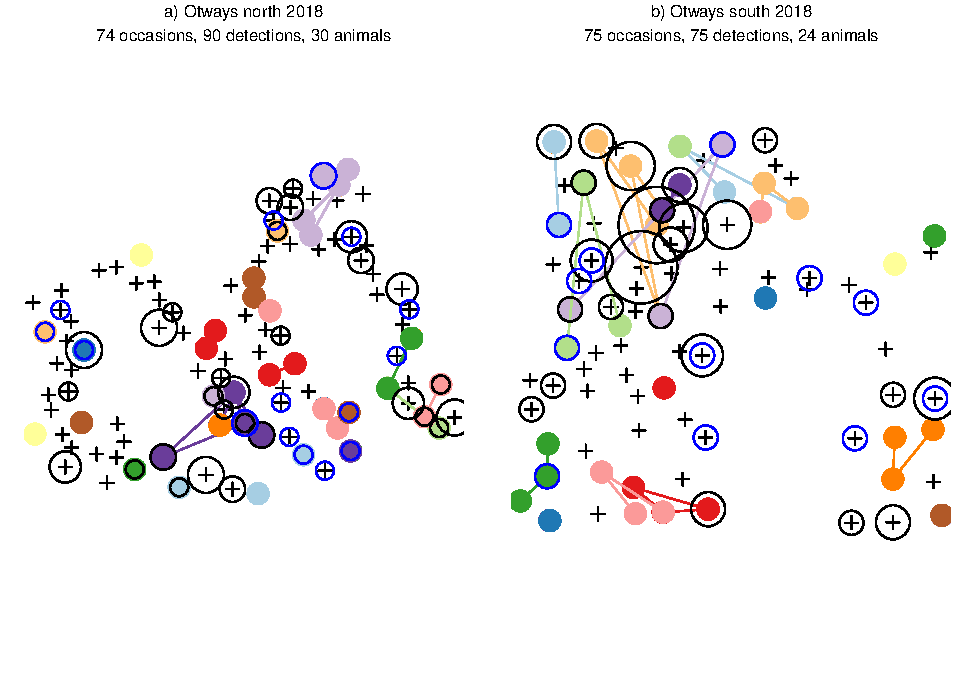
\includegraphics[width=1\linewidth]{figure/density-plot-ch-5-1} 

}

\caption{Feral cat detections in the Otway region, Australia, 2018. Solid fill coloured circles represent identified cats with lines indicating observed movements. Black open circles indicate black cat detections; blue circles indicate unidentifiable tabby cat detections, with circle radius scaling positively with the number of daily detections. Fox control had occurred, but lapsed just prior to the survey in the northern landscape (a), and did not occur in the southern landscape (b).}\label{fig:density-plot-ch-5}
\end{figure}
\newpage

\hypertarget{section-2}{%
\subsubsection{2019}\label{section-2}}

\(~\)

\(~\)

\(~\)
\begin{figure}

{\centering 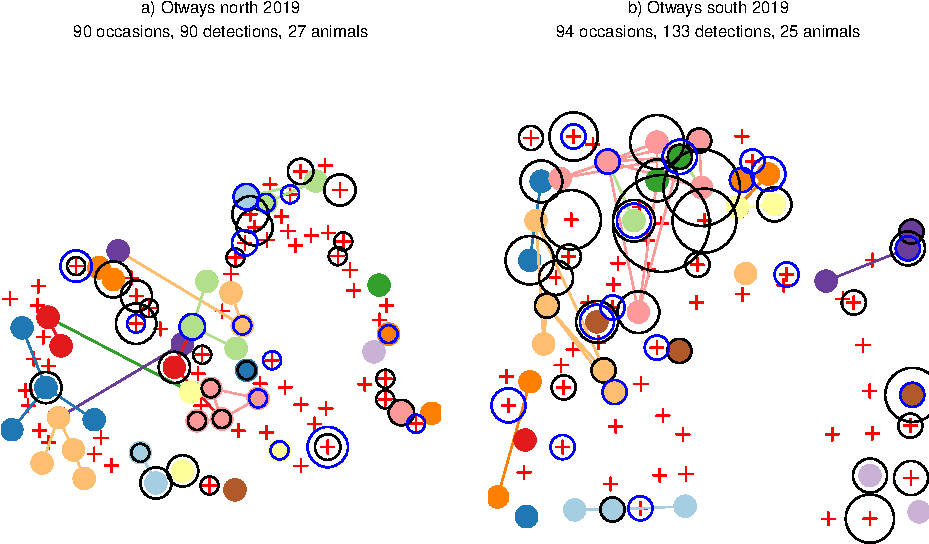
\includegraphics[width=1\linewidth]{figure/density-plot-ch-6-1} 

}

\caption{Feral cat detections in the Otway region, Australia, 2019. Solid fill coloured circles represent identified cats with lines indicating observed movements. Black open circles indicate black cat detections; blue circles indicate unidentifiable tabby cat detections, with circle radius scaling positively with the number of daily detections. Fox control occurred in the northern landscape (a) during this survey, but not the southern landscape (b).}\label{fig:density-plot-ch-6}
\end{figure}
\newpage

\hypertarget{density-app-fox}{%
\section{Fox spatial occurrence}\label{density-app-fox}}

\hypertarget{glenelg-region-4}{%
\subsection{Glenelg region}\label{glenelg-region-4}}

\(~\)

\(~\)

\(~\)
\begin{verbatim}

Family: binomial 
Link function: logit 

Formula:
fox ~ s(x, y, bs = "ds", m = c(1, 0.5), k = 200) + offset(log(survey_duration))

Parametric coefficients:
            Estimate Std. Error z value Pr(>|z|)    
(Intercept) -4.53965    0.09293  -48.85   <2e-16 ***
---
Signif. codes:  0 '***' 0.001 '**' 0.01 '*' 0.05 '.' 0.1 ' ' 1

Approximate significance of smooth terms:
         edf Ref.df Chi.sq  p-value    
s(x,y) 25.58    199  61.78 9.75e-07 ***
---
Signif. codes:  0 '***' 0.001 '**' 0.01 '*' 0.05 '.' 0.1 ' ' 1

R-sq.(adj) =  0.126   Deviance explained = 13.1%
fREML = 845.52  Scale est. = 1         n = 538
\end{verbatim}
\newpage

\(~\)

\(~\)

\(~\)
\begin{figure}

{\centering 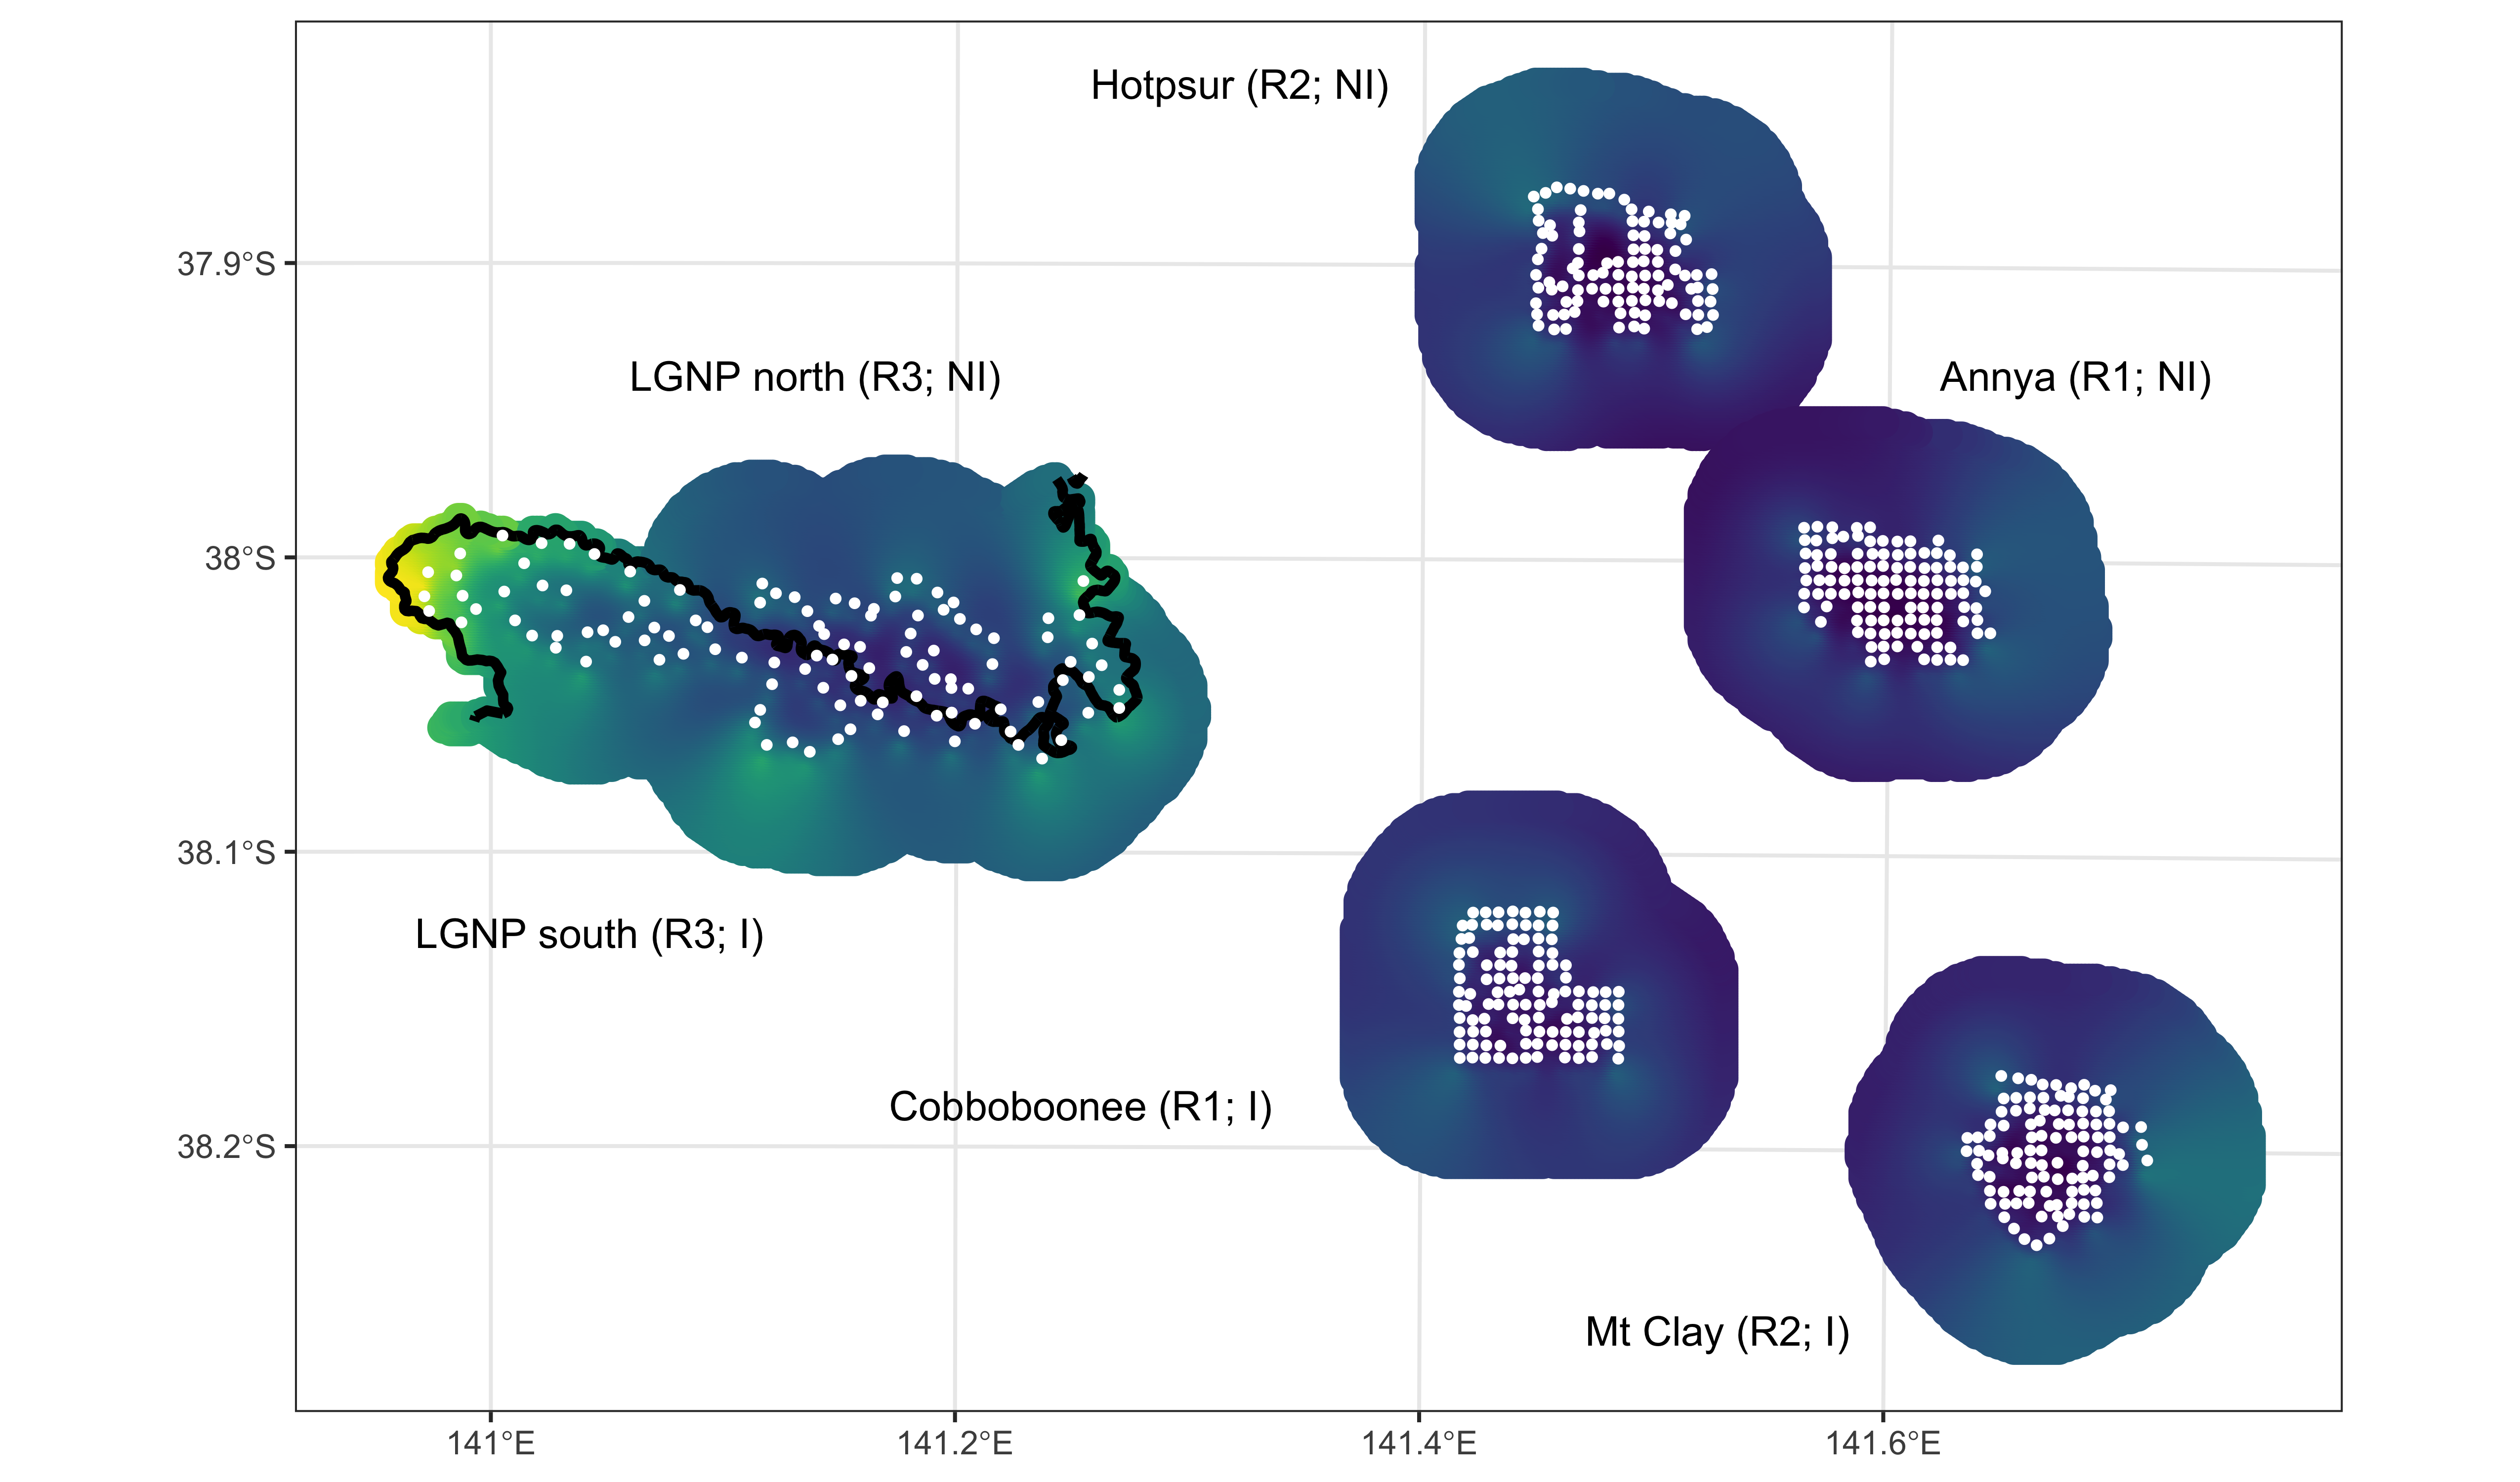
\includegraphics[width=1\linewidth]{figure/fox_occ_se_glenelg_600dpi} 

}

\caption{Standard error estimate of log fox occurrence probability derived from generalised additive models within each impact (I) and associated non-impact (NI) landscape in the Glenelg region, Australia.}\label{fig:density-fox-se-g}
\end{figure}
\newpage

\hypertarget{otway-region-1}{%
\subsection{Otway Region}\label{otway-region-1}}

\(~\)

\(~\)

\(~\)
\begin{verbatim}

Family: binomial 
Link function: logit 

Formula:
fox ~ year + s(x, y, by = year, bs = "ds", m = c(1, 0.5), k = 100) + 
    s(station, bs = "re") + offset(log(survey_duration))

Parametric coefficients:
             Estimate Std. Error z value Pr(>|z|)    
(Intercept) -5.283154   0.230023 -22.968   <2e-16 ***
year2018     0.004643   0.277696   0.017    0.987    
year2019     0.037119   0.282270   0.132    0.895    
---
Signif. codes:  0 '***' 0.001 '**' 0.01 '*' 0.05 '.' 0.1 ' ' 1

Approximate significance of smooth terms:
                      edf Ref.df Chi.sq  p-value    
s(x,y):year2017 2.688e+00     99  8.096 0.010597 *  
s(x,y):year2018 2.494e-05     99  0.000 0.506341    
s(x,y):year2019 6.148e+00     99 22.262 0.000380 ***
s(station)      5.366e+01    194 75.723 0.000116 ***
---
Signif. codes:  0 '***' 0.001 '**' 0.01 '*' 0.05 '.' 0.1 ' ' 1

R-sq.(adj) =   0.24   Deviance explained = 27.8%
fREML = 763.36  Scale est. = 1         n = 513
\end{verbatim}
\newpage

\(~\)

\(~\)

\(~\)
\begin{figure}

{\centering 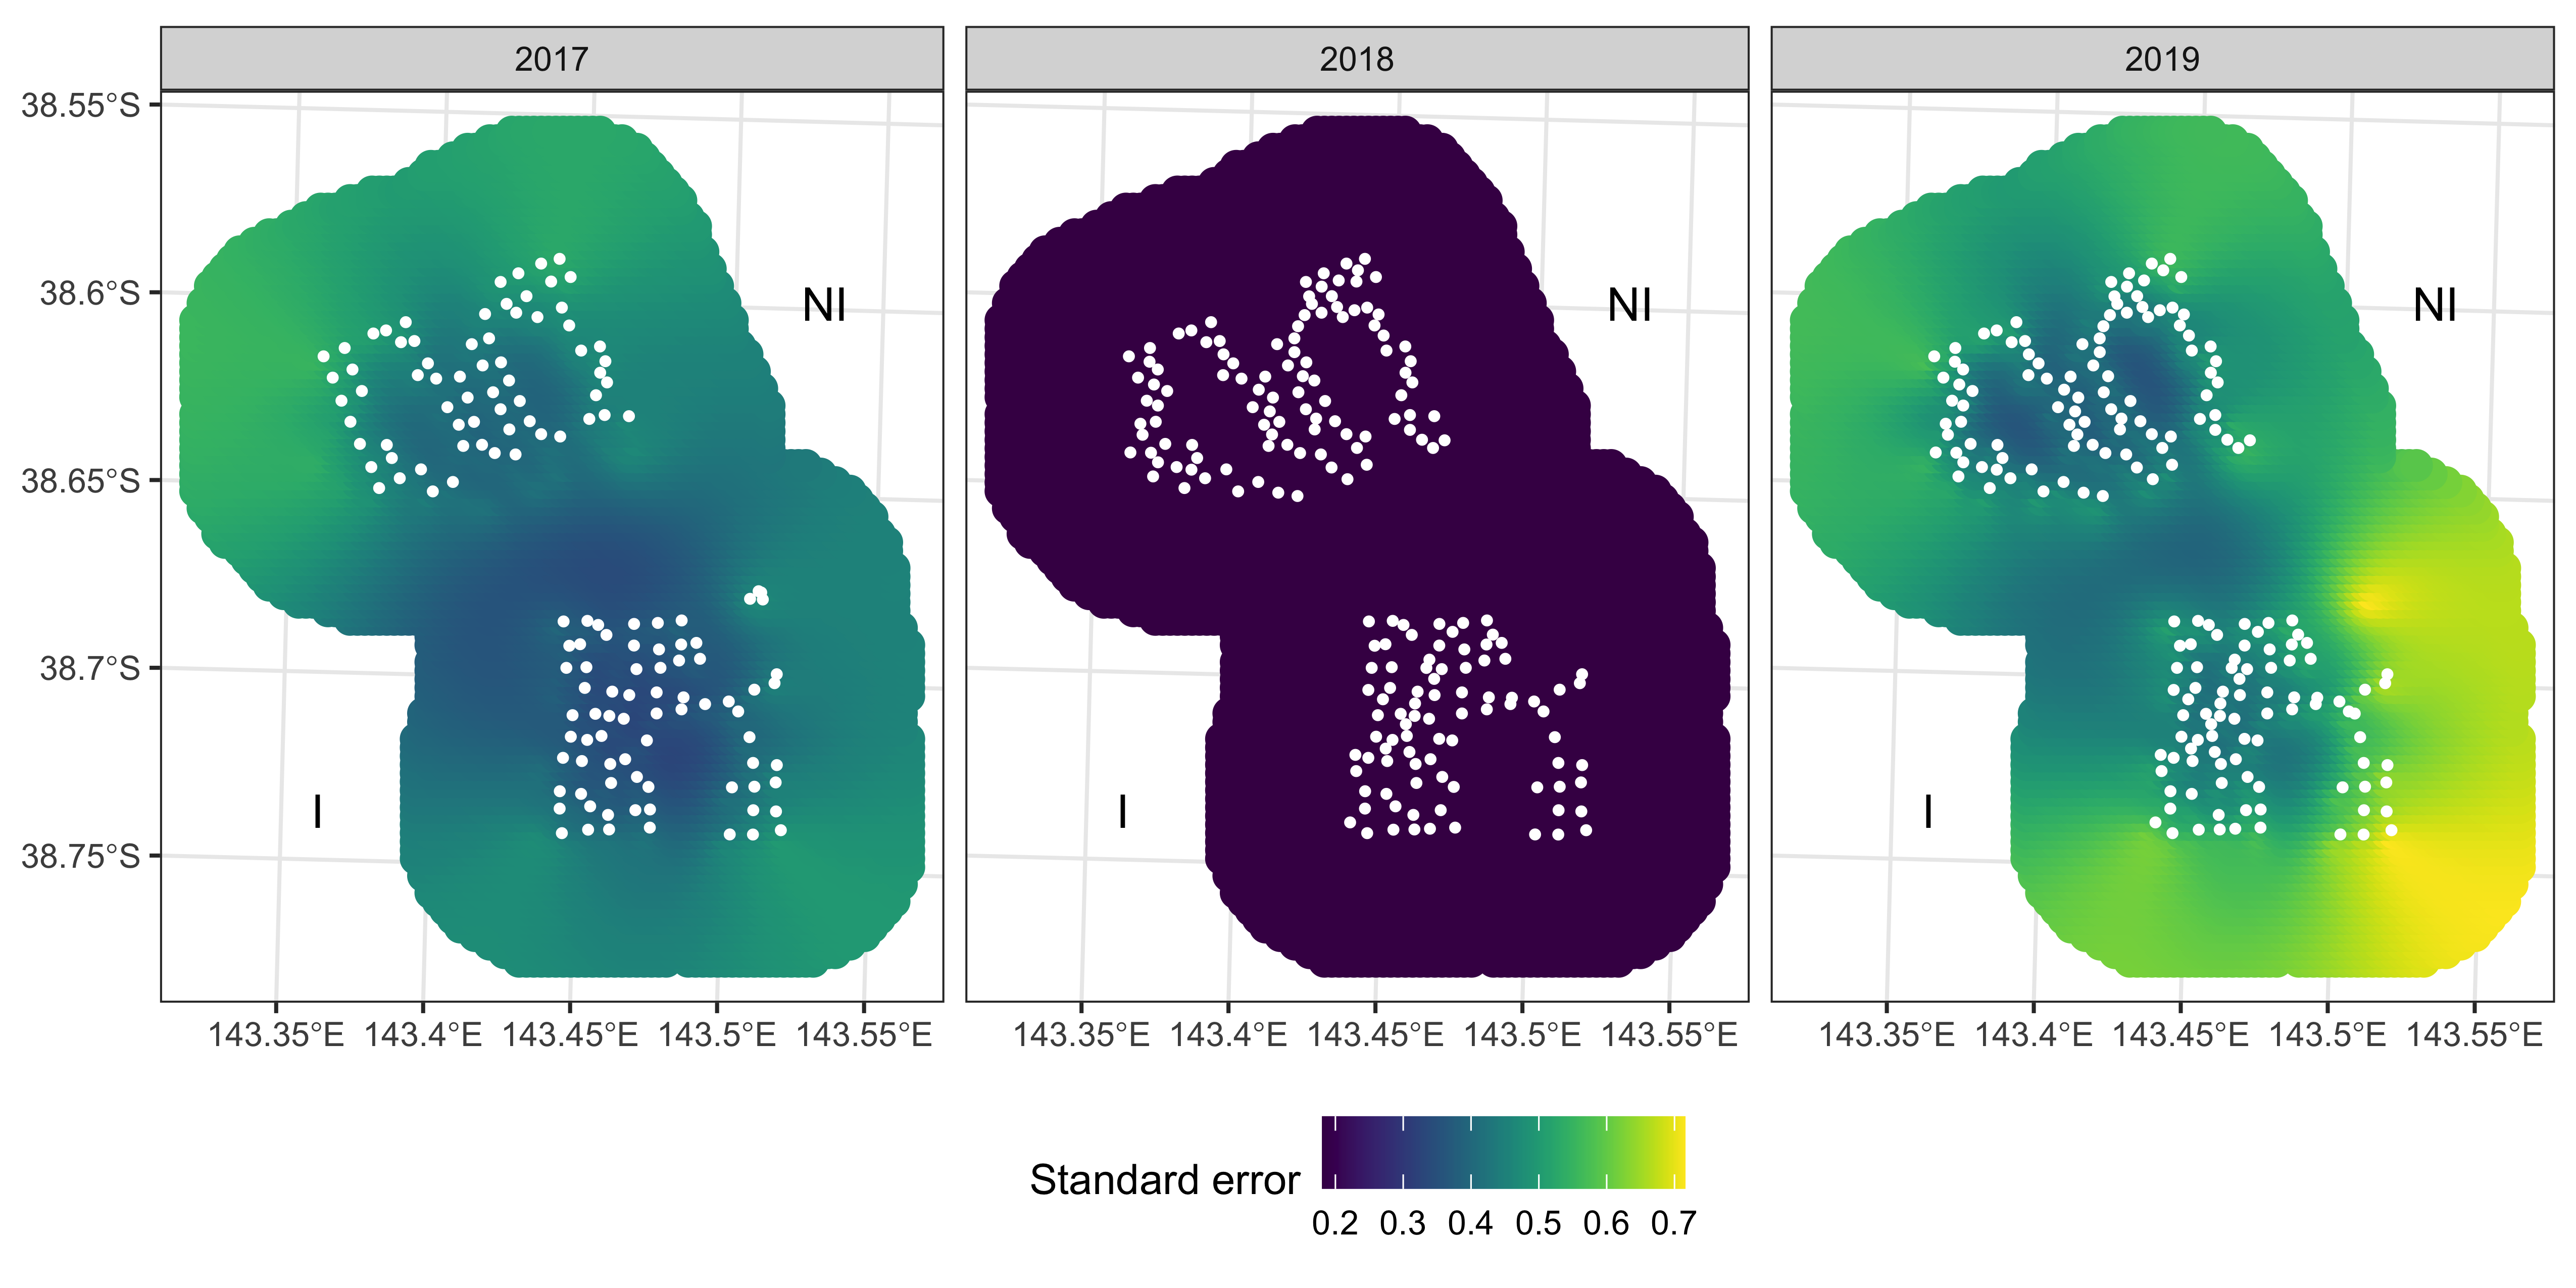
\includegraphics[width=1\linewidth]{figure/fox_occ_se_otways_600dpi} 

}

\caption{Standard error estimate of log fox occurrence probability derived from generalised additive models within each impact (I) and associated non-impact (NI) landscape in the Otway region, Australia.}\label{fig:density-fox-se-o}
\end{figure}
\newpage

\hypertarget{density-app-veg}{%
\section{Vegetation categories}\label{density-app-veg}}

We condensed the main Ecological Vegetation Class groupings ({\textbf{???}}) present into three categories for each region: cleared land, heathy woodlands, lowland forests (Glenelg region only) and wet forests (Otways region only). We merged similar groups to reduce the number of categories for each region. In the Glenelg region, we merged dry forests with lowland forests. In the Otway region, we merged rainforests with wet forests, as well as merged dry forests and heathy woodlands.

A very small proportion of other Ecological Vegetation Class groupings were present in the habitat masks: riparian scrubs or swampy scrubs and woodlands, coastal scrubs grasslands and woodlands, wetlands, riverine grassy woodlands or forests, plains woodlands or forests, herb-rich woodlands. We removed these groups, and interpolated cell values from the nearest of the three vegetation categories.

\newpage

\(~\)

\(~\)

\(~\)
\begin{figure}

{\centering 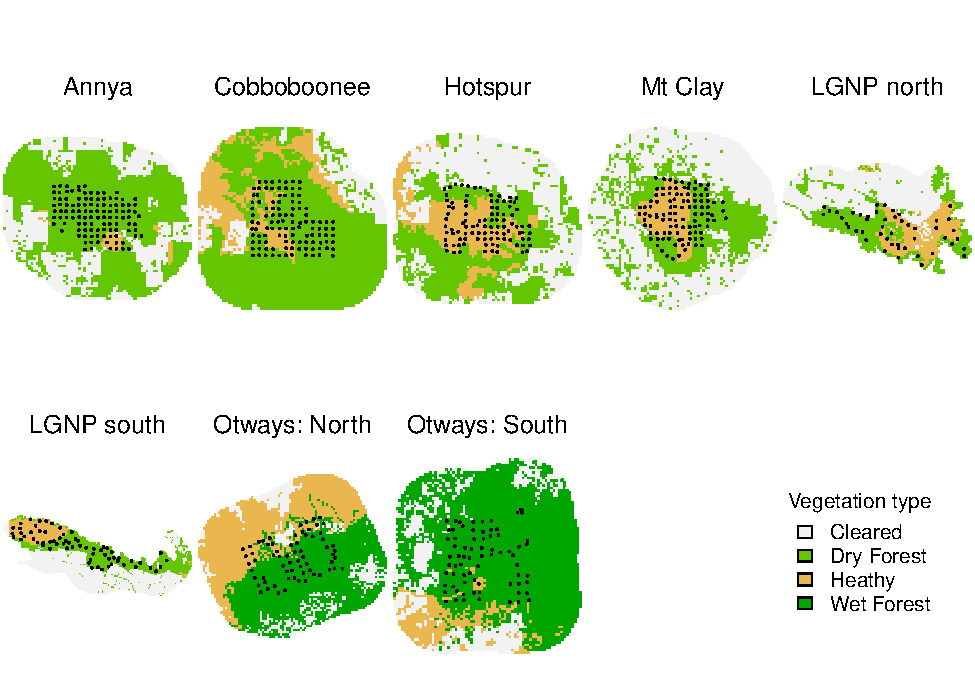
\includegraphics[width=1\linewidth]{figure/density-veg-1} 

}

\caption{Condensed Ecological Vegetation Class groups used as habitat mask covariates in spatial mark-resight models.}\label{fig:density-veg}
\end{figure}
\newpage

\hypertarget{spatial-mark-resight-models}{%
\section{Spatial mark-resight models}\label{spatial-mark-resight-models}}

\hypertarget{glenelg-region-5}{%
\subsection{Glenelg region}\label{glenelg-region-5}}

\(~\)

\(~\)

\(~\)

\begingroup\fontsize{10}{12}\selectfont
\begin{longtable}[t]{lrrrrrr}
\caption{\label{tab:density-aic-g-1}Akaike's Information Criterion values adjusted for small sample size for feral cat density models in the Glenelg region; model set 1.}\\
\toprule
Detector function & K & logLik & AIC & AICc & dAICc & AICcwt\\
\midrule
exponential & 3 & -1745.99 & 3497.99 & 3498.37 & 0.00 & 1\\
half-normal & 3 & -1763.02 & 3532.05 & 3532.43 & 34.06 & 0\\
\bottomrule
\multicolumn{7}{l}{\rule{0pt}{1em}K - number of parameters}\\
\multicolumn{7}{l}{\rule{0pt}{1em}AICc - Akaike's Information Criterion with small-sample adjustment}\\
\multicolumn{7}{l}{\rule{0pt}{1em}dAICc - difference between AICc of this model and the model with smallest AICc}\\
\multicolumn{7}{l}{\rule{0pt}{1em}AICcwt - AICc model weight}\\
\end{longtable}
\endgroup{}

\newpage

\(~\)

\(~\)

\(~\)

\begingroup\fontsize{10}{12}\selectfont
\begin{longtable}[t]{lrrrrrr}
\caption{\label{tab:density-aic-g-2}Akaike's Information Criterion values adjusted for small sample size for feral cat density models in the Glenelg region; model set 2.}\\
\toprule
Model & K & logLik & AIC & AICc & dAICc & AICcwt\\
\midrule
D\textasciitilde{}1 g0\textasciitilde{}1 sigma\textasciitilde{}1 & 3 & -1309.93 & 2625.85 & 2626.23 & 0.00 & 0.32\\
D\textasciitilde{}vegetation g0\textasciitilde{}1 sigma\textasciitilde{}1 & 5 & -1307.68 & 2625.37 & 2626.35 & 0.12 & 0.30\\
D\textasciitilde{}vegetation g0\textasciitilde{}T sigma\textasciitilde{}1 & 6 & -1306.89 & 2625.77 & 2627.17 & 0.94 & 0.20\\
D\textasciitilde{}1 g0\textasciitilde{}T sigma\textasciitilde{}1 & 4 & -1309.32 & 2626.65 & 2627.29 & 1.06 & 0.19\\
\bottomrule
\multicolumn{7}{l}{\rule{0pt}{1em}K - number of parameters}\\
\multicolumn{7}{l}{\rule{0pt}{1em}AICc - Akaike's Information Criterion with small-sample adjustment}\\
\multicolumn{7}{l}{\rule{0pt}{1em}dAICc - difference between AICc of this model and the model with smallest AICc}\\
\multicolumn{7}{l}{\rule{0pt}{1em}AICcwt - AICc model weight}\\
\multicolumn{7}{l}{\rule{0pt}{1em}T - linear time trend (g0 only)}\\
\end{longtable}
\endgroup{}

\newpage

\(~\)

\(~\)

\(~\)

\begingroup\fontsize{10}{12}\selectfont
\begin{longtable}[t]{lrrrrrr}
\caption{\label{tab:density-aic-g-3}Akaike's Information Criterion values adjusted for small sample size for feral cat density models in the Glenelg region; model set 3.}\\
\toprule
Model & K & logLik & AIC & AICc & dAICc & AICcwt\\
\midrule
D\textasciitilde{}fox\_occ g0\textasciitilde{}1 sigma\textasciitilde{}1 & 4 & -1306.67 & 2621.33 & 2621.98 & 0.00 & 0.49\\
D\textasciitilde{}fox\_occ g0\textasciitilde{}fox\_occ sigma\textasciitilde{}fox\_occ & 6 & -1304.97 & 2621.94 & 2623.34 & 1.36 & 0.25\\
D\textasciitilde{}s(fox\_occ) g0\textasciitilde{}1 sigma\textasciitilde{}1 & 5 & -1306.61 & 2623.21 & 2624.20 & 2.22 & 0.16\\
D\textasciitilde{}1 g0\textasciitilde{}1 sigma\textasciitilde{}1 & 3 & -1309.93 & 2625.85 & 2626.23 & 4.26 & 0.06\\
D\textasciitilde{}s(fox\_occ) g0\textasciitilde{}s(fox\_occ) sigma\textasciitilde{}s(fox\_occ) & 9 & -1303.41 & 2624.81 & 2627.97 & 5.99 & 0.02\\
\addlinespace
D\textasciitilde{}1 g0\textasciitilde{}fox\_occ sigma\textasciitilde{}fox\_occ & 5 & -1309.41 & 2628.82 & 2629.80 & 7.82 & 0.01\\
D\textasciitilde{}1 g0\textasciitilde{}s(fox\_occ) sigma\textasciitilde{}s(fox\_occ) & 7 & -1307.91 & 2629.81 & 2631.71 & 9.73 & 0.00\\
\bottomrule
\multicolumn{7}{l}{\rule{0pt}{1em}K - number of parameters}\\
\multicolumn{7}{l}{\rule{0pt}{1em}AICc - Akaike's Information Criterion with small-sample adjustment}\\
\multicolumn{7}{l}{\rule{0pt}{1em}dAICc - difference between AICc of this model and the model with smallest AICc}\\
\multicolumn{7}{l}{\rule{0pt}{1em}AICcwt - AICc model weight}\\
\multicolumn{7}{l}{\rule{0pt}{1em}fox\_occ - fine-scale occurrence probability of foxes derived from generalised additive models}\\
\multicolumn{7}{l}{\rule{0pt}{1em}s(fox\_occ) - non-linear smooth of fox\_occ with three knots}\\
\end{longtable}
\endgroup{}

\newpage

\(~\)

\(~\)

\(~\)

\begingroup\fontsize{10}{12}\selectfont
\begin{longtable}[t]{lrrrrrr}
\caption{\label{tab:density-aic-g-4}Akaike's Information Criterion values adjusted for small sample size for feral cat density models in the Glenelg region; model set 4.}\\
\toprule
Model & K & logLik & AIC & AICc & dAICc & AICcwt\\
\midrule
D\textasciitilde{}session g0\textasciitilde{}fox\_occ sigma\textasciitilde{}fox\_occ & 10 & -1297.46 & 2614.93 & 2618.86 & 0.00 & 0.62\\
D\textasciitilde{}session g0\textasciitilde{}1 sigma\textasciitilde{}1 & 8 & -1300.66 & 2617.32 & 2619.80 & 0.95 & 0.38\\
\bottomrule
\multicolumn{7}{l}{\rule{0pt}{1em}K - number of parameters}\\
\multicolumn{7}{l}{\rule{0pt}{1em}AICc - Akaike's Information Criterion with small-sample adjustment}\\
\multicolumn{7}{l}{\rule{0pt}{1em}dAICc - difference between AICc of this model and the model with smallest AICc}\\
\multicolumn{7}{l}{\rule{0pt}{1em}AICcwt - AICc model weight}\\
\multicolumn{7}{l}{\rule{0pt}{1em}fox\_occ - fine-scale occurrence probability of foxes derived from generalised additive models}\\
\multicolumn{7}{l}{\rule{0pt}{1em}session - landscape (n = 6)}\\
\end{longtable}
\endgroup{}

\newpage

\(~\)

\(~\)

\(~\)

\begingroup\fontsize{10}{12}\selectfont
\begin{longtable}[t]{lrrrll}
\caption{\label{tab:density-landscape-est}Feral cat density per square kilometre as estimated by the AICc top-ranked model in the Glenelg region, Australia.}\\
\toprule
Landscape & Estimate & 5\% CI & 95\% CI & Treatment & Replicate\\
\midrule
Annya & 0.24 & 0.17 & 0.34 & Non-impact & 1\\
Cobboboonee & 0.60 & 0.40 & 0.88 & Impact & 1\\
Hotspur & 0.22 & 0.14 & 0.33 & Non-impact & 2\\
Mt Clay & 0.24 & 0.18 & 0.31 & Impact & 2\\
LGNP north & 0.15 & 0.07 & 0.35 & Non-impact & 3\\
\addlinespace
LGNP south & 0.56 & 0.34 & 0.90 & Impact & 3\\
\bottomrule
\end{longtable}
\endgroup{}

\newpage

\hypertarget{otway-region-2}{%
\subsection{Otway region}\label{otway-region-2}}

\(~\)

\(~\)

\(~\)

\begingroup\fontsize{10}{12}\selectfont
\begin{longtable}[t]{lrrrrrr}
\caption{\label{tab:density-aic-o-1}Akaike's Information Criterion values for detector functions in the Otway region, Australia; model set 1.}\\
\toprule
Detector function & K & logLik & AIC & AICc & dAICc & AICcwt\\
\midrule
exponential & 3 & -5591.00 & 11188.01 & 11188.17 & 0.00 & 1\\
half-normal & 3 & -5743.26 & 11492.52 & 11492.69 & 304.52 & 0\\
\bottomrule
\multicolumn{7}{l}{\rule{0pt}{1em}K - number of parameters}\\
\multicolumn{7}{l}{\rule{0pt}{1em}AICc - Akaike's Information Criterion with small-sample adjustment}\\
\multicolumn{7}{l}{\rule{0pt}{1em}dAICc - difference between AICc of this model and the model with smallest AICc}\\
\multicolumn{7}{l}{\rule{0pt}{1em}AICcwt - AICc model weight}\\
\end{longtable}
\endgroup{}

\newpage

\(~\)

\(~\)

\(~\)

\begingroup\fontsize{10}{12}\selectfont
\begin{longtable}[t]{lrrrrrr}
\caption{\label{tab:density-aic-o-2}Akaike's Information Criterion values adjusted for small sample size for feral cat density models in the Otway region; model set 2.}\\
\toprule
Model & K & logLik & AIC & AICc & dAICc & AICcwt\\
\midrule
D\textasciitilde{}year g0\textasciitilde{}1 sigma\textasciitilde{}1 & 5 & -3550.63 & 7111.26 & 7111.67 & 0.00 & 0.48\\
D\textasciitilde{}year g0\textasciitilde{}T sigma\textasciitilde{}1 & 6 & -3549.83 & 7111.67 & 7112.25 & 0.57 & 0.36\\
D\textasciitilde{}year + vegetation g0\textasciitilde{}1 sigma\textasciitilde{}1 & 7 & -3550.04 & 7114.08 & 7114.86 & 3.19 & 0.10\\
D\textasciitilde{}year + vegetation g0\textasciitilde{}T sigma\textasciitilde{}1 & 8 & -3549.24 & 7114.48 & 7115.49 & 3.82 & 0.07\\
\bottomrule
\multicolumn{7}{l}{\rule{0pt}{1em}K - number of parameters}\\
\multicolumn{7}{l}{\rule{0pt}{1em}AICc - Akaike's Information Criterion with small-sample adjustment}\\
\multicolumn{7}{l}{\rule{0pt}{1em}dAICc - difference between AICc of this model and the model with smallest AICc}\\
\multicolumn{7}{l}{\rule{0pt}{1em}AICcwt - AICc model weight}\\
\multicolumn{7}{l}{\rule{0pt}{1em}T - linear time trend (g0 only)}\\
\end{longtable}
\endgroup{}

\newpage

\(~\)

\(~\)

\(~\)

\begingroup\fontsize{10}{12}\selectfont
\begin{longtable}[t]{lrrrrrr}
\caption{\label{tab:density-aic-o-3}Akaike's Information Criterion values adjusted for small sample size for feral cat density models in the Otway region; model set 3.}\\
\toprule
Model & K & logLik & AIC & AICc & dAICc & AICcwt\\
\midrule
D\textasciitilde{}year + fox\_occ g0\textasciitilde{}fox\_occ sigma\textasciitilde{}fox\_occ & 8 & -3541.80 & 7099.59 & 7100.60 & 0.00 & 0.33\\
D\textasciitilde{}year + s(fox\_occ) g0\textasciitilde{}s(fox\_occ) sigma\textasciitilde{}s(fox\_occ) & 11 & -3538.59 & 7099.19 & 7101.07 & 0.47 & 0.26\\
D\textasciitilde{}year g0\textasciitilde{}s(fox\_occ) sigma\textasciitilde{}s(fox\_occ) & 9 & -3541.07 & 7100.13 & 7101.40 & 0.80 & 0.22\\
D\textasciitilde{}year g0\textasciitilde{}fox\_occ sigma\textasciitilde{}fox\_occ & 7 & -3543.44 & 7100.87 & 7101.65 & 1.05 & 0.19\\
D\textasciitilde{}year + fox\_occ g0\textasciitilde{}1 sigma\textasciitilde{}1 & 6 & -3548.26 & 7108.51 & 7109.09 & 8.49 & 0.00\\
\addlinespace
D\textasciitilde{}year + s(fox\_occ) g0\textasciitilde{}1 sigma\textasciitilde{}1 & 7 & -3547.47 & 7108.94 & 7109.72 & 9.12 & 0.00\\
D\textasciitilde{}year g0\textasciitilde{}1 sigma\textasciitilde{}1 & 5 & -3550.63 & 7111.26 & 7111.67 & 11.07 & 0.00\\
\bottomrule
\multicolumn{7}{l}{\rule{0pt}{1em}K - number of parameters}\\
\multicolumn{7}{l}{\rule{0pt}{1em}AICc - Akaike's Information Criterion with small-sample adjustment}\\
\multicolumn{7}{l}{\rule{0pt}{1em}dAICc - difference between AICc of this model and the model with smallest AICc}\\
\multicolumn{7}{l}{\rule{0pt}{1em}AICcwt - AICc model weight}\\
\multicolumn{7}{l}{\rule{0pt}{1em}fox\_occ - fine-scale occurrence probability of foxes derived from generalised additive models}\\
\multicolumn{7}{l}{\rule{0pt}{1em}s(fox\_occ) - non-linear smooth of fox\_occ with three knots}\\
\end{longtable}
\endgroup{}

\newpage

\(~\)

\(~\)

\(~\)

\begingroup\fontsize{10}{12}\selectfont
\begin{longtable}[t]{lrrrrrr}
\caption{\label{tab:density-aic-o-4}Akaike's Information Criterion values adjusted for small sample size for feral cat density models in the Otway region; model set 4.}\\
\toprule
Model & K & logLik & AIC & AICc & dAICc & AICcwt\\
\midrule
D\textasciitilde{}session g0\textasciitilde{}fox\_occ sigma\textasciitilde{}fox\_occ & 10 & -3541.77 & 7103.55 & 7105.11 & 0.00 & 0.99\\
D\textasciitilde{}session g0\textasciitilde{}1 sigma\textasciitilde{}1 & 8 & -3548.37 & 7112.73 & 7113.74 & 8.63 & 0.01\\
\bottomrule
\multicolumn{7}{l}{\rule{0pt}{1em}K - number of parameters}\\
\multicolumn{7}{l}{\rule{0pt}{1em}AICc - Akaike's Information Criterion with small-sample adjustment}\\
\multicolumn{7}{l}{\rule{0pt}{1em}dAICc - difference between AICc of this model and the model with smallest AICc}\\
\multicolumn{7}{l}{\rule{0pt}{1em}AICcwt - AICc model weight}\\
\multicolumn{7}{l}{\rule{0pt}{1em}fox\_occ - fine-scale occurrence probability of foxes derived from generalised additive models}\\
\multicolumn{7}{l}{\rule{0pt}{1em}session - landscape by year (n = 6)}\\
\end{longtable}
\endgroup{}

\newpage

\(~\)

\(~\)

\(~\)

\begingroup\fontsize{10}{12}\selectfont
\begin{longtable}[t]{lrrrll}
\caption{\label{tab:density-aic-o-5}Feral cat density per square kilometre as estimated by the AICc top-ranked model in the Otway region, Australia.}\\
\toprule
Landscape & Estimate & 5\% CI & 95\% CI & Treatment & Year\\
\midrule
north 2017 & 1.00 & 0.74 & 1.35 & Non-impact & 2017\\
south 2017 & 0.74 & 0.52 & 1.05 & Impact & 2017\\
north 2018 & 0.81 & 0.64 & 1.02 & Non-impact & 2018\\
south 2018 & 0.82 & 0.63 & 1.06 & Impact & 2018\\
north 2019 & 0.73 & 0.55 & 0.95 & Non-impact & 2019\\
\addlinespace
south 2019 & 0.98 & 0.76 & 1.27 & Impact & 2019\\
\bottomrule
\end{longtable}
\endgroup{}

\newpage

\hypertarget{diel-app}{%
\chapter{Supporting Information: Chapter \ref{diel}}\label{diel-app}}

\newpage

\(~\)

\(~\)

\(~\)

\begingroup\fontsize{10}{12}\selectfont
\begin{longtable}[t]{llrrrr}
\caption{\label{tab:diel-tab1}Summary of the number of camera-trap deployments, unique survey sites and 'independent' counts of invasive predator detections across Ecological Vegetation Class groups within the Glenelg and Otway regions, south-west Victoria, Australia.}\\
\toprule
Vegetation & Region & Sites & Deployments & Fox counts & Cat counts\\
\midrule
Dry Forest & Glenelg & 25 & 69 & 347 & 9\\
 & Otways & 111 & 314 & 341 & 158\\
Heathland & Glenelg & 40 & 119 & 265 & 59\\
 & Otways & 3 & 9 & 8 & 6\\
Heathy Woodland & Glenelg & 154 & 424 & 574 & 96\\
\addlinespace
 & Otways & 82 & 256 & 160 & 66\\
Herb-rich Woodland & Glenelg & 59 & 373 & 863 & 198\\
 & Otways & 2 & 6 & 3 & 2\\
Lowland Forest & Glenelg & 383 & 1046 & 1900 & 290\\
 & Otways & 52 & 163 & 190 & 35\\
\addlinespace
Swampy Scrub & Glenelg & 4 & 10 & 19 & 8\\
 & Otways & 36 & 98 & 64 & 88\\
Wet Forest & Otways & 281 & 780 & 715 & 1187\\
\textbf{Total} & \textbf{} & \textbf{1232} & \textbf{3667} & \textbf{5449} & \textbf{2202}\\
\bottomrule
\end{longtable}
\endgroup{}

\newpage

\begingroup\fontsize{10}{12}\selectfont
\begin{longtable}[t]{llrrr}
\caption{\label{tab:diel-tab-fits}Generalised additive model summaries for invasive predator spatiotemporal activity in south-west Victoria, Australia.}\\
\toprule
Species & Model & EDF & dev.expl & r.sq\\
\midrule
fox & 1\_spatial & 772.6469 & 0.3514 & 0.1170\\
fox & 2\_vegetation\_type & 766.1054 & 0.3498 & 0.1155\\
fox & 3\_habitat\_type & 768.2692 & 0.3487 & 0.1139\\
cat & 1\_spatial & 562.9236 & 0.2314 & 0.0772\\
cat & 2\_vegetation\_type & 566.7562 & 0.2300 & 0.0769\\
\addlinespace
cat & 3\_fox\_by\_habitat\_type & 587.9491 & 0.2322 & 0.0789\\
\bottomrule
\multicolumn{5}{l}{\rule{0pt}{1em}\textit{Note: }}\\
\multicolumn{5}{l}{\rule{0pt}{1em}EDF - estimated degrees of freedom of all model terms.}\\
\multicolumn{5}{l}{\rule{0pt}{1em}dev.expl - proportion of the null deviance explained by the model. }\\
\multicolumn{5}{l}{\rule{0pt}{1em}r.sq -  adjusted r-squared value.}\\
\end{longtable}
\endgroup{}

\newpage
\begin{figure}

{\centering 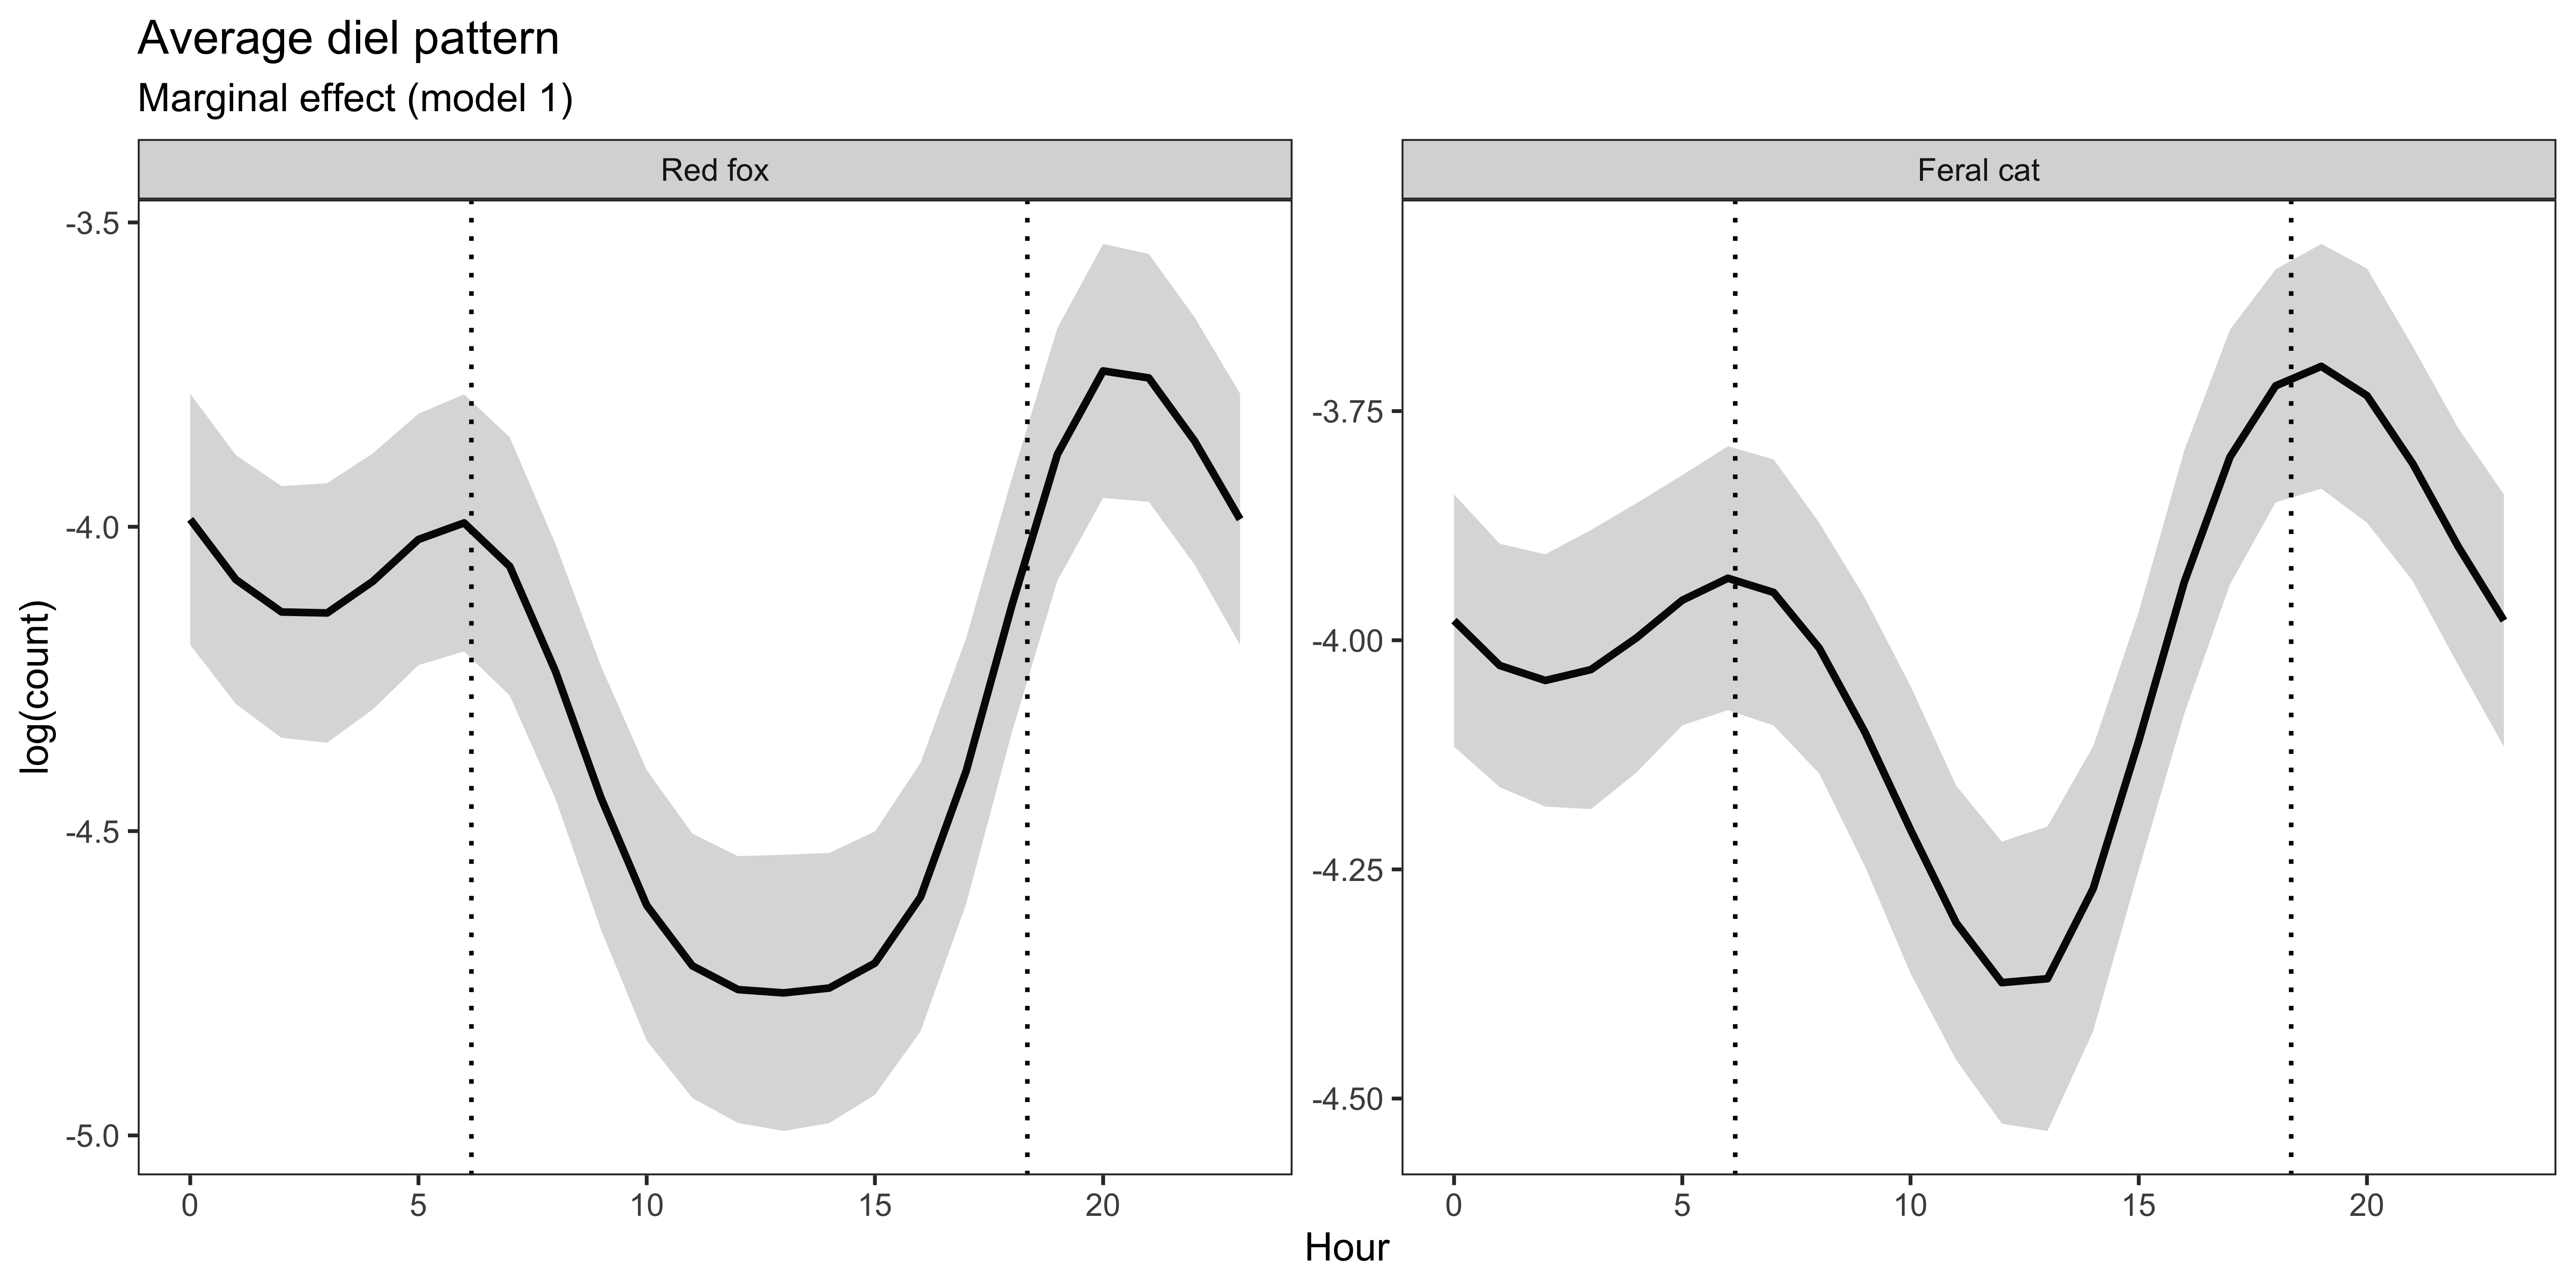
\includegraphics[width=1\linewidth]{figure/avg_diel_predator} 

}

\caption{Marginal effect of time (model 1) on predators across both study regions in south-west Victoria, Australia. White crosses depict unique camera-trap sites}\label{fig:diel-space-time-marginal}
\end{figure}
\newpage
\begin{center}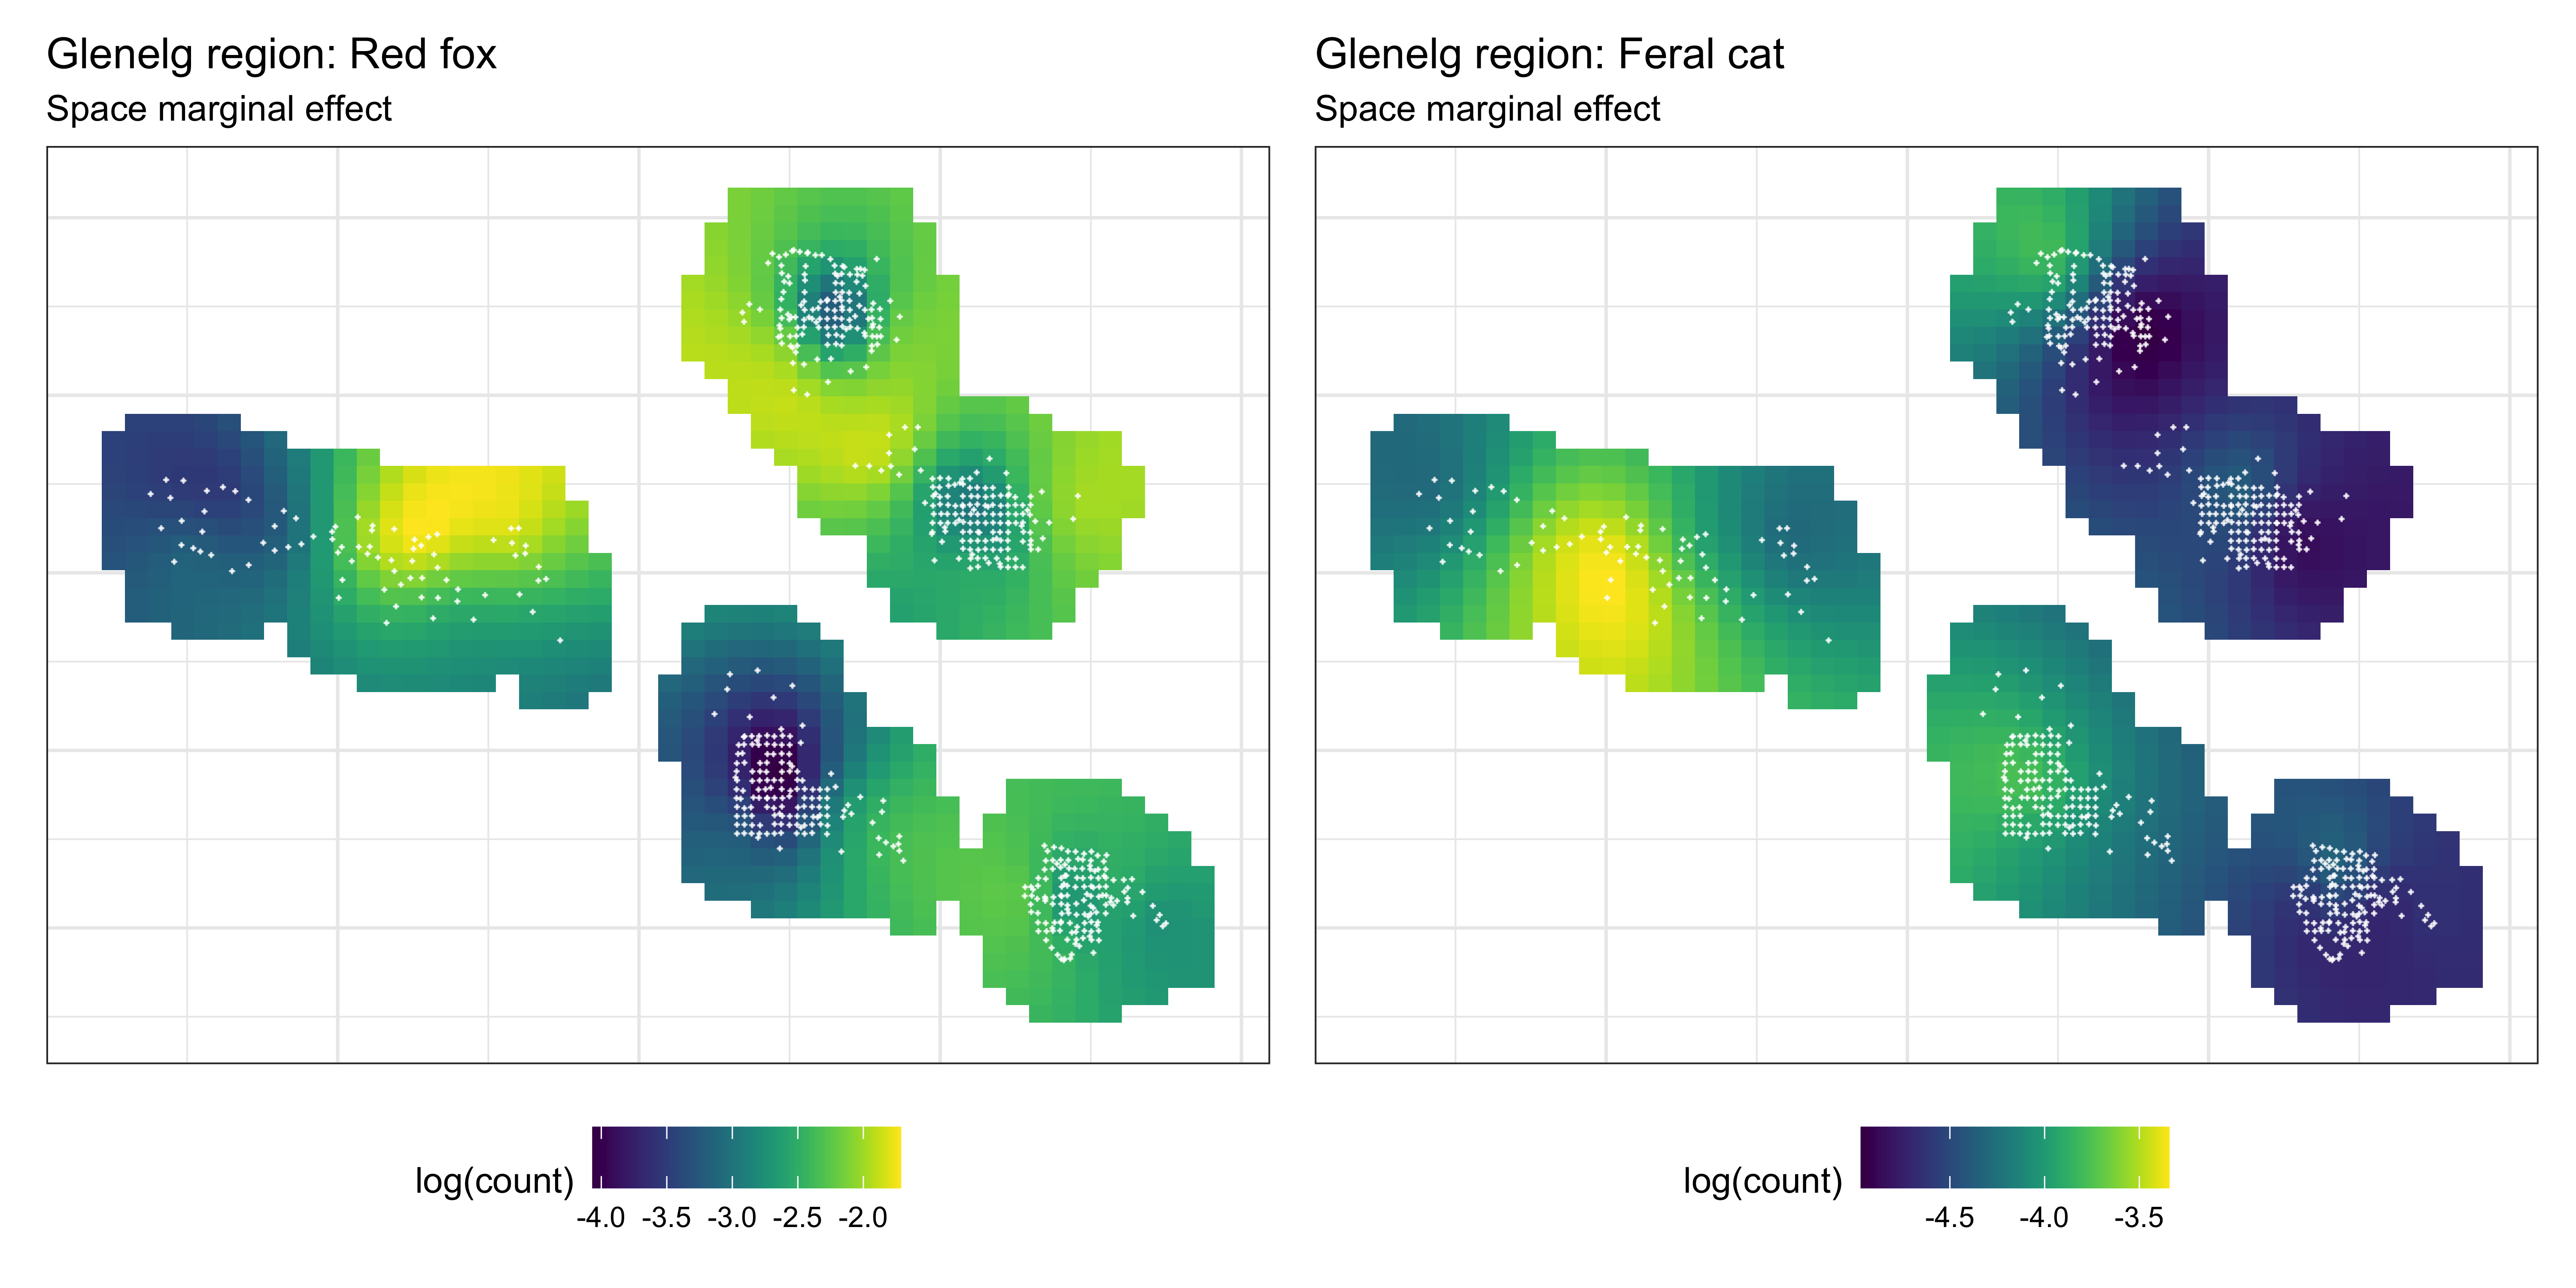
\includegraphics[width=1\linewidth]{figure/sp_marginal_g} \end{center}
\begin{figure}

{\centering 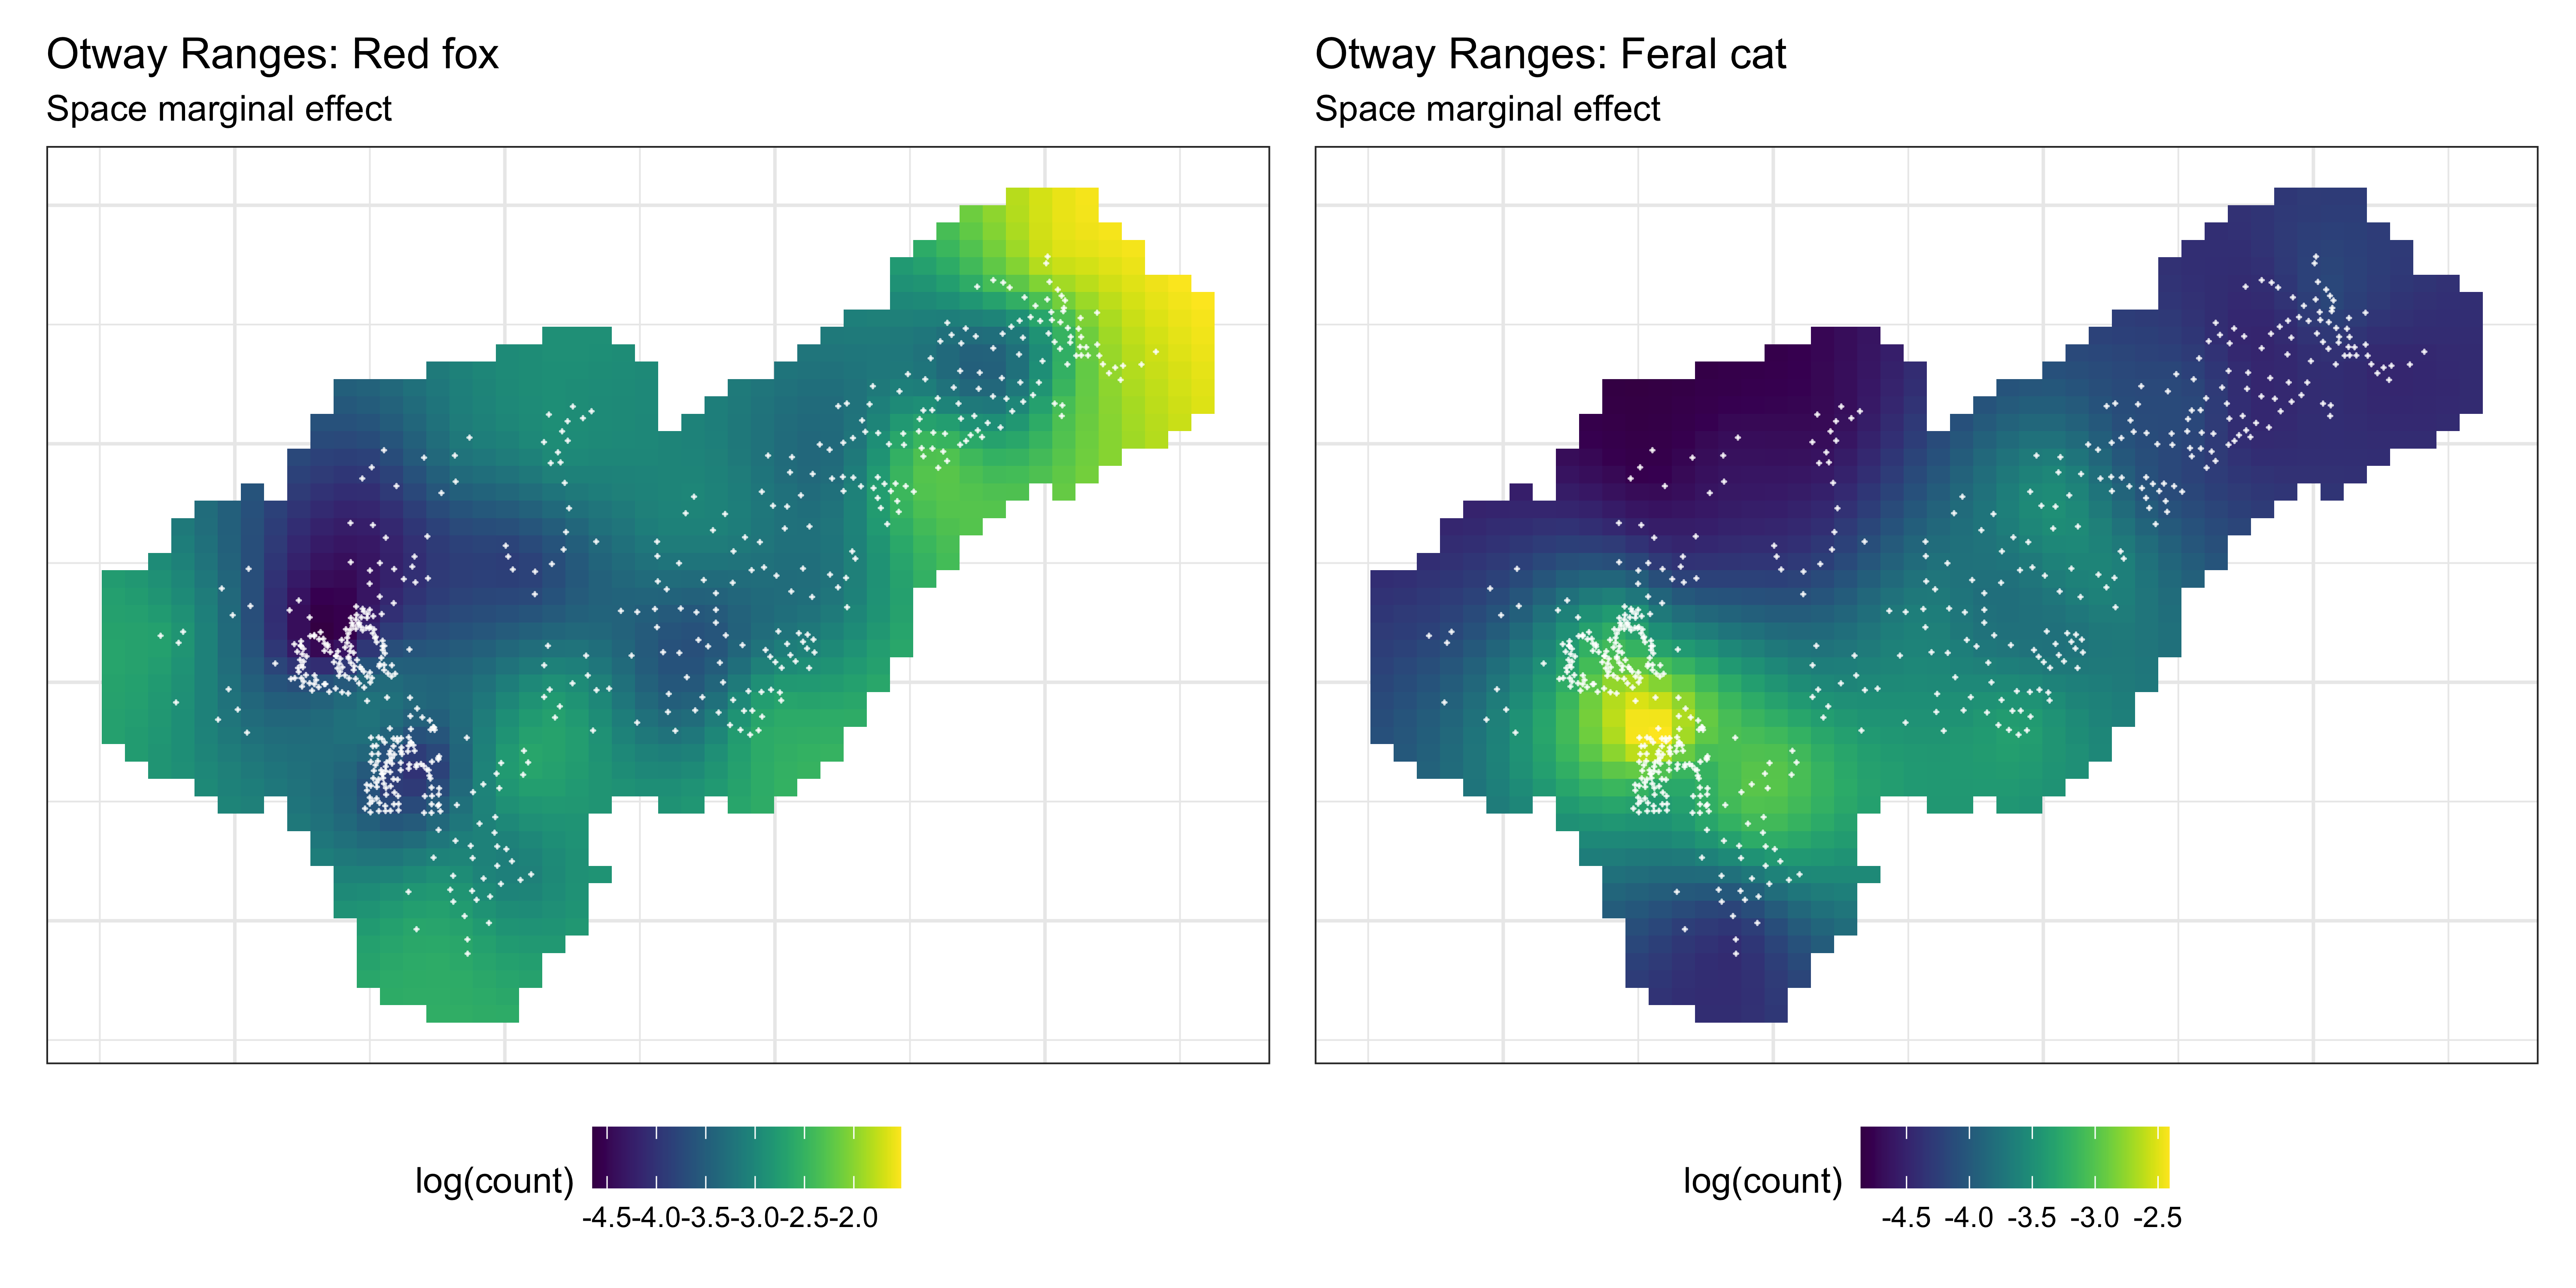
\includegraphics[width=1\linewidth]{figure/sp_marginal_o} 

}

\caption{Marginal effect of space on predators across south-west Victoria, Australia (model 1). White crosses depict unique camera-trap sites}\label{fig:diel-space-time-marginal-o}
\end{figure}
\newpage
\begin{figure}

{\centering 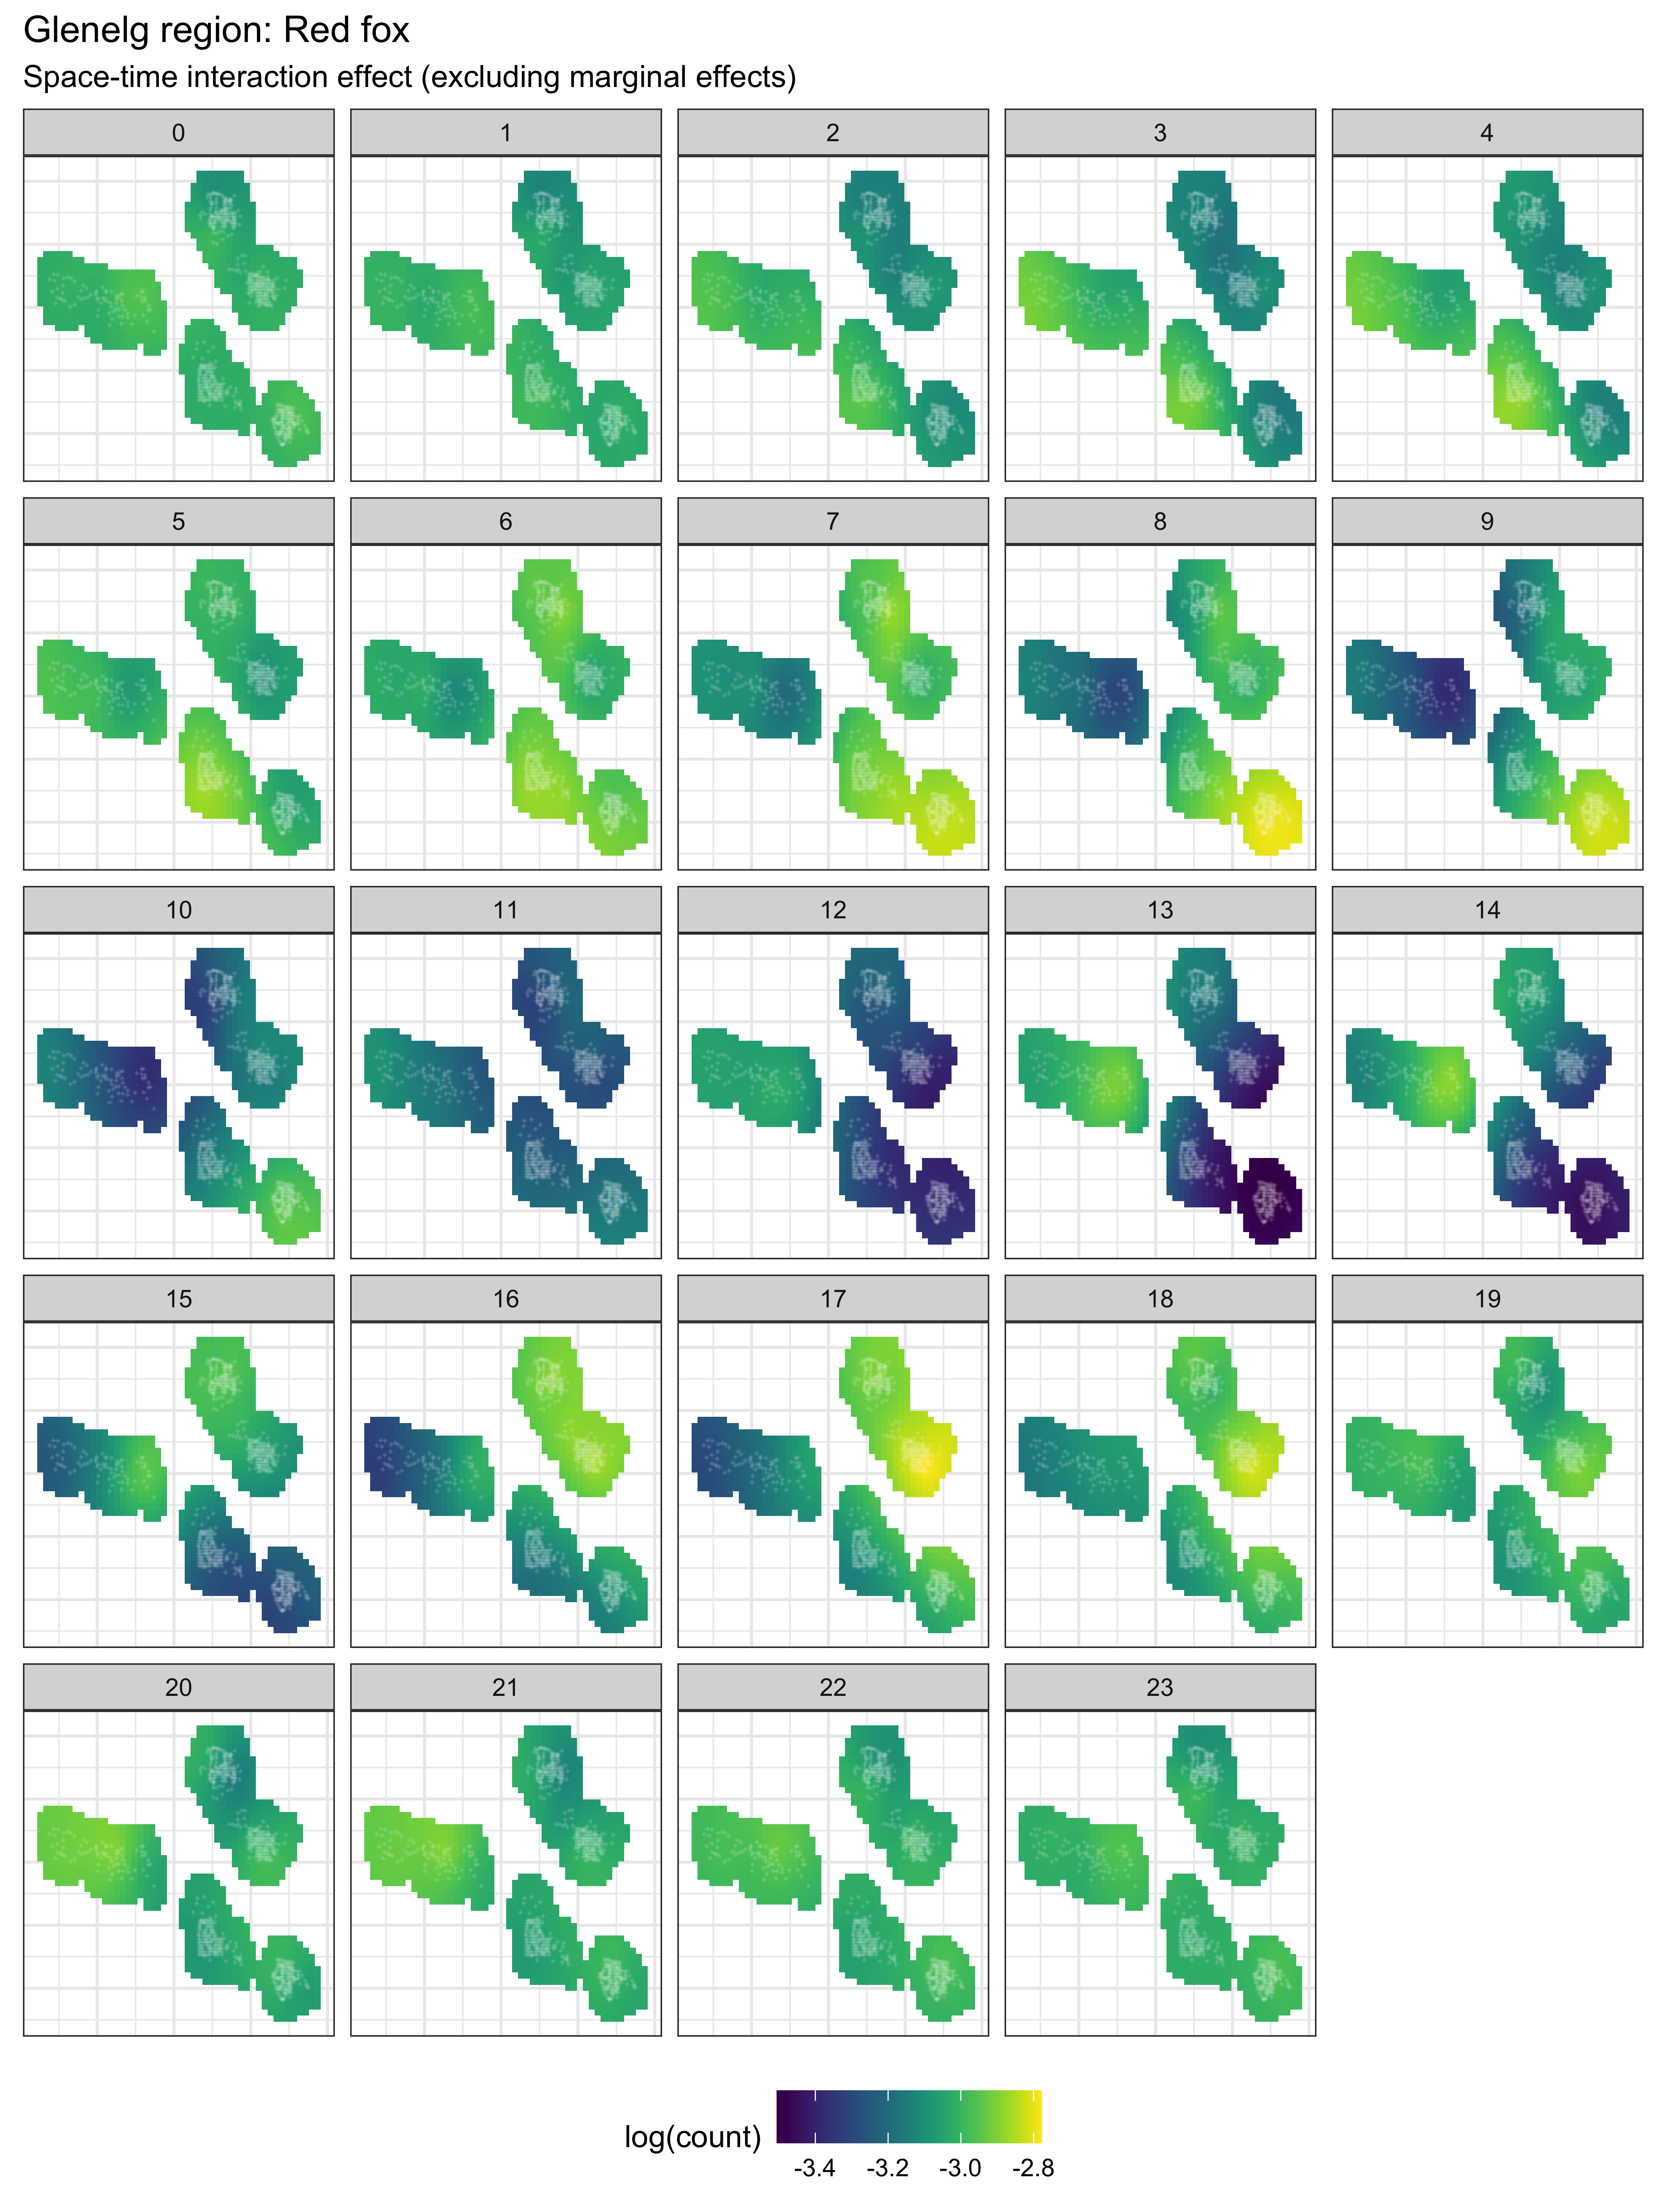
\includegraphics[width=1\linewidth]{figure/spte_diff_avg_g_fox} 

}

\caption{Interaction effect of space-time on feral cat \textit{Felis catus} activity across each hour of the day (0 - 23) in the Glenelg region, Australia (model 1). White crosses depict unique camera-trap sites. }\label{fig:diel-st-int-g-fox}
\end{figure}
\newpage
\begin{figure}

{\centering 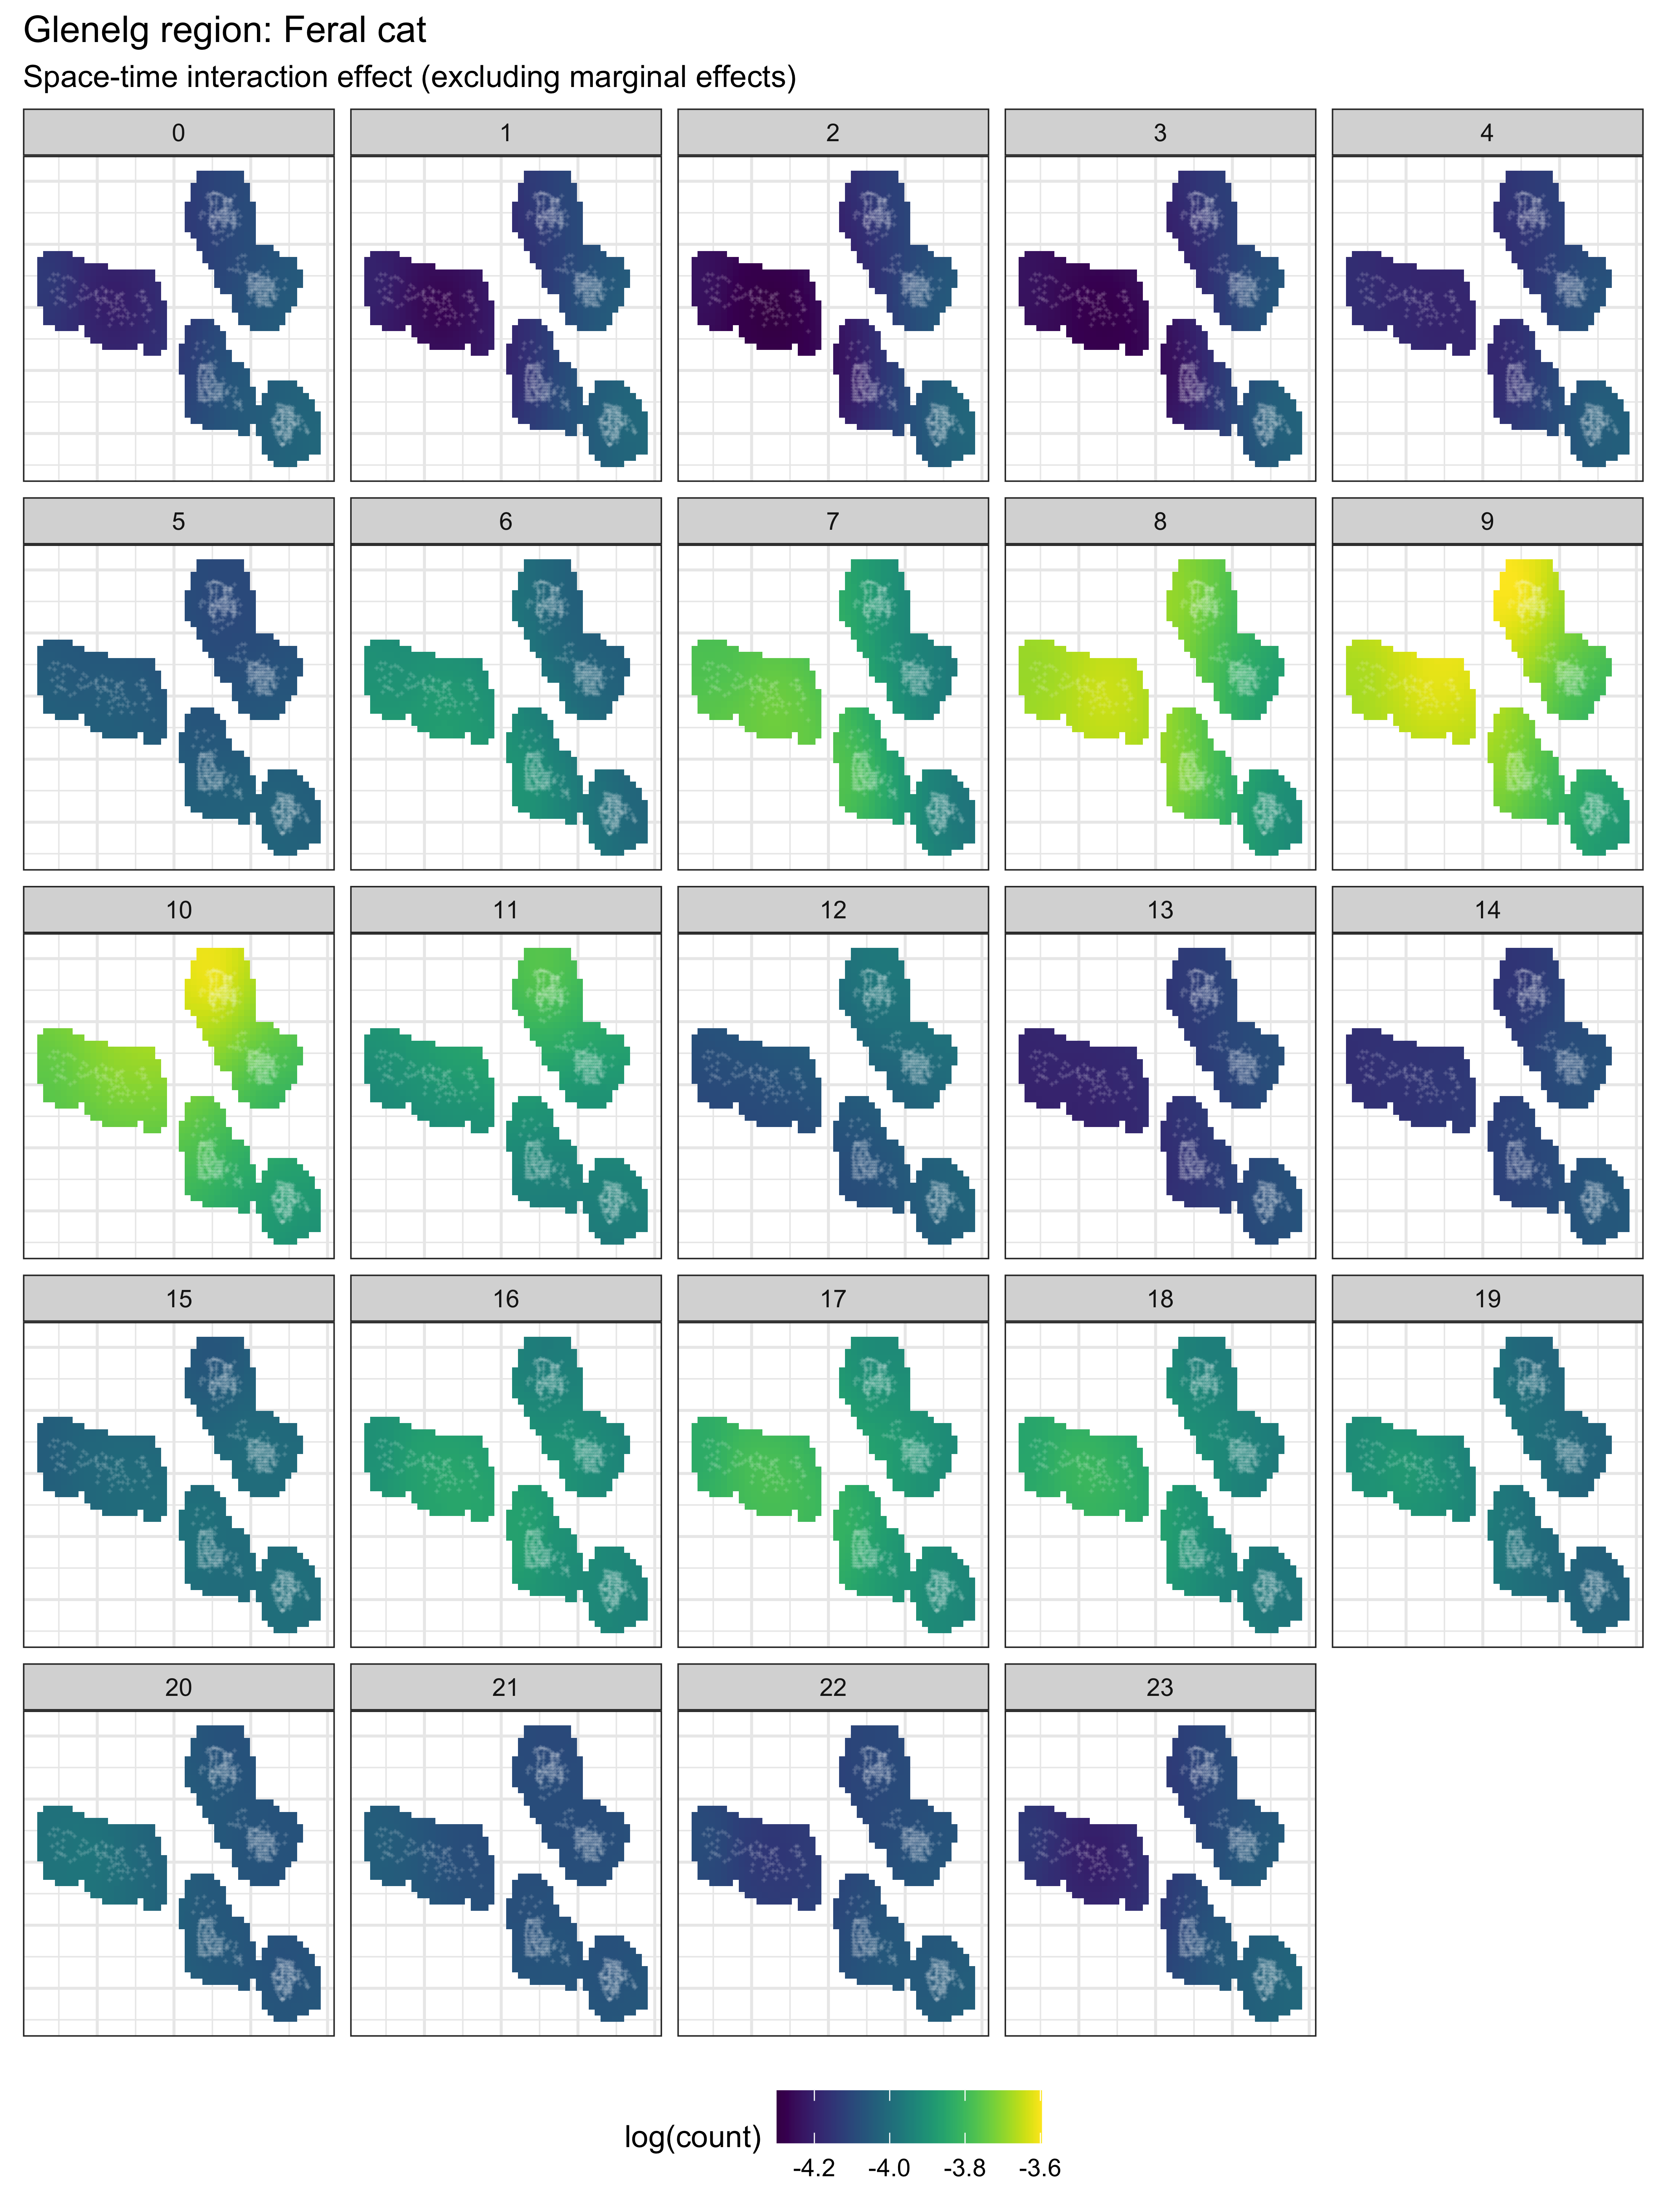
\includegraphics[width=1\linewidth]{figure/spte_diff_avg_g_cat} 

}

\caption{Interaction effect of space-time on feral cat \textit{Felis catus} activity across each hour of the day (0 - 23) in the Glenelg region, Australia (model 1). White crosses depict unique camera-trap sites. }\label{fig:diel-st-int-g-cat}
\end{figure}
\newpage
\begin{figure}

{\centering 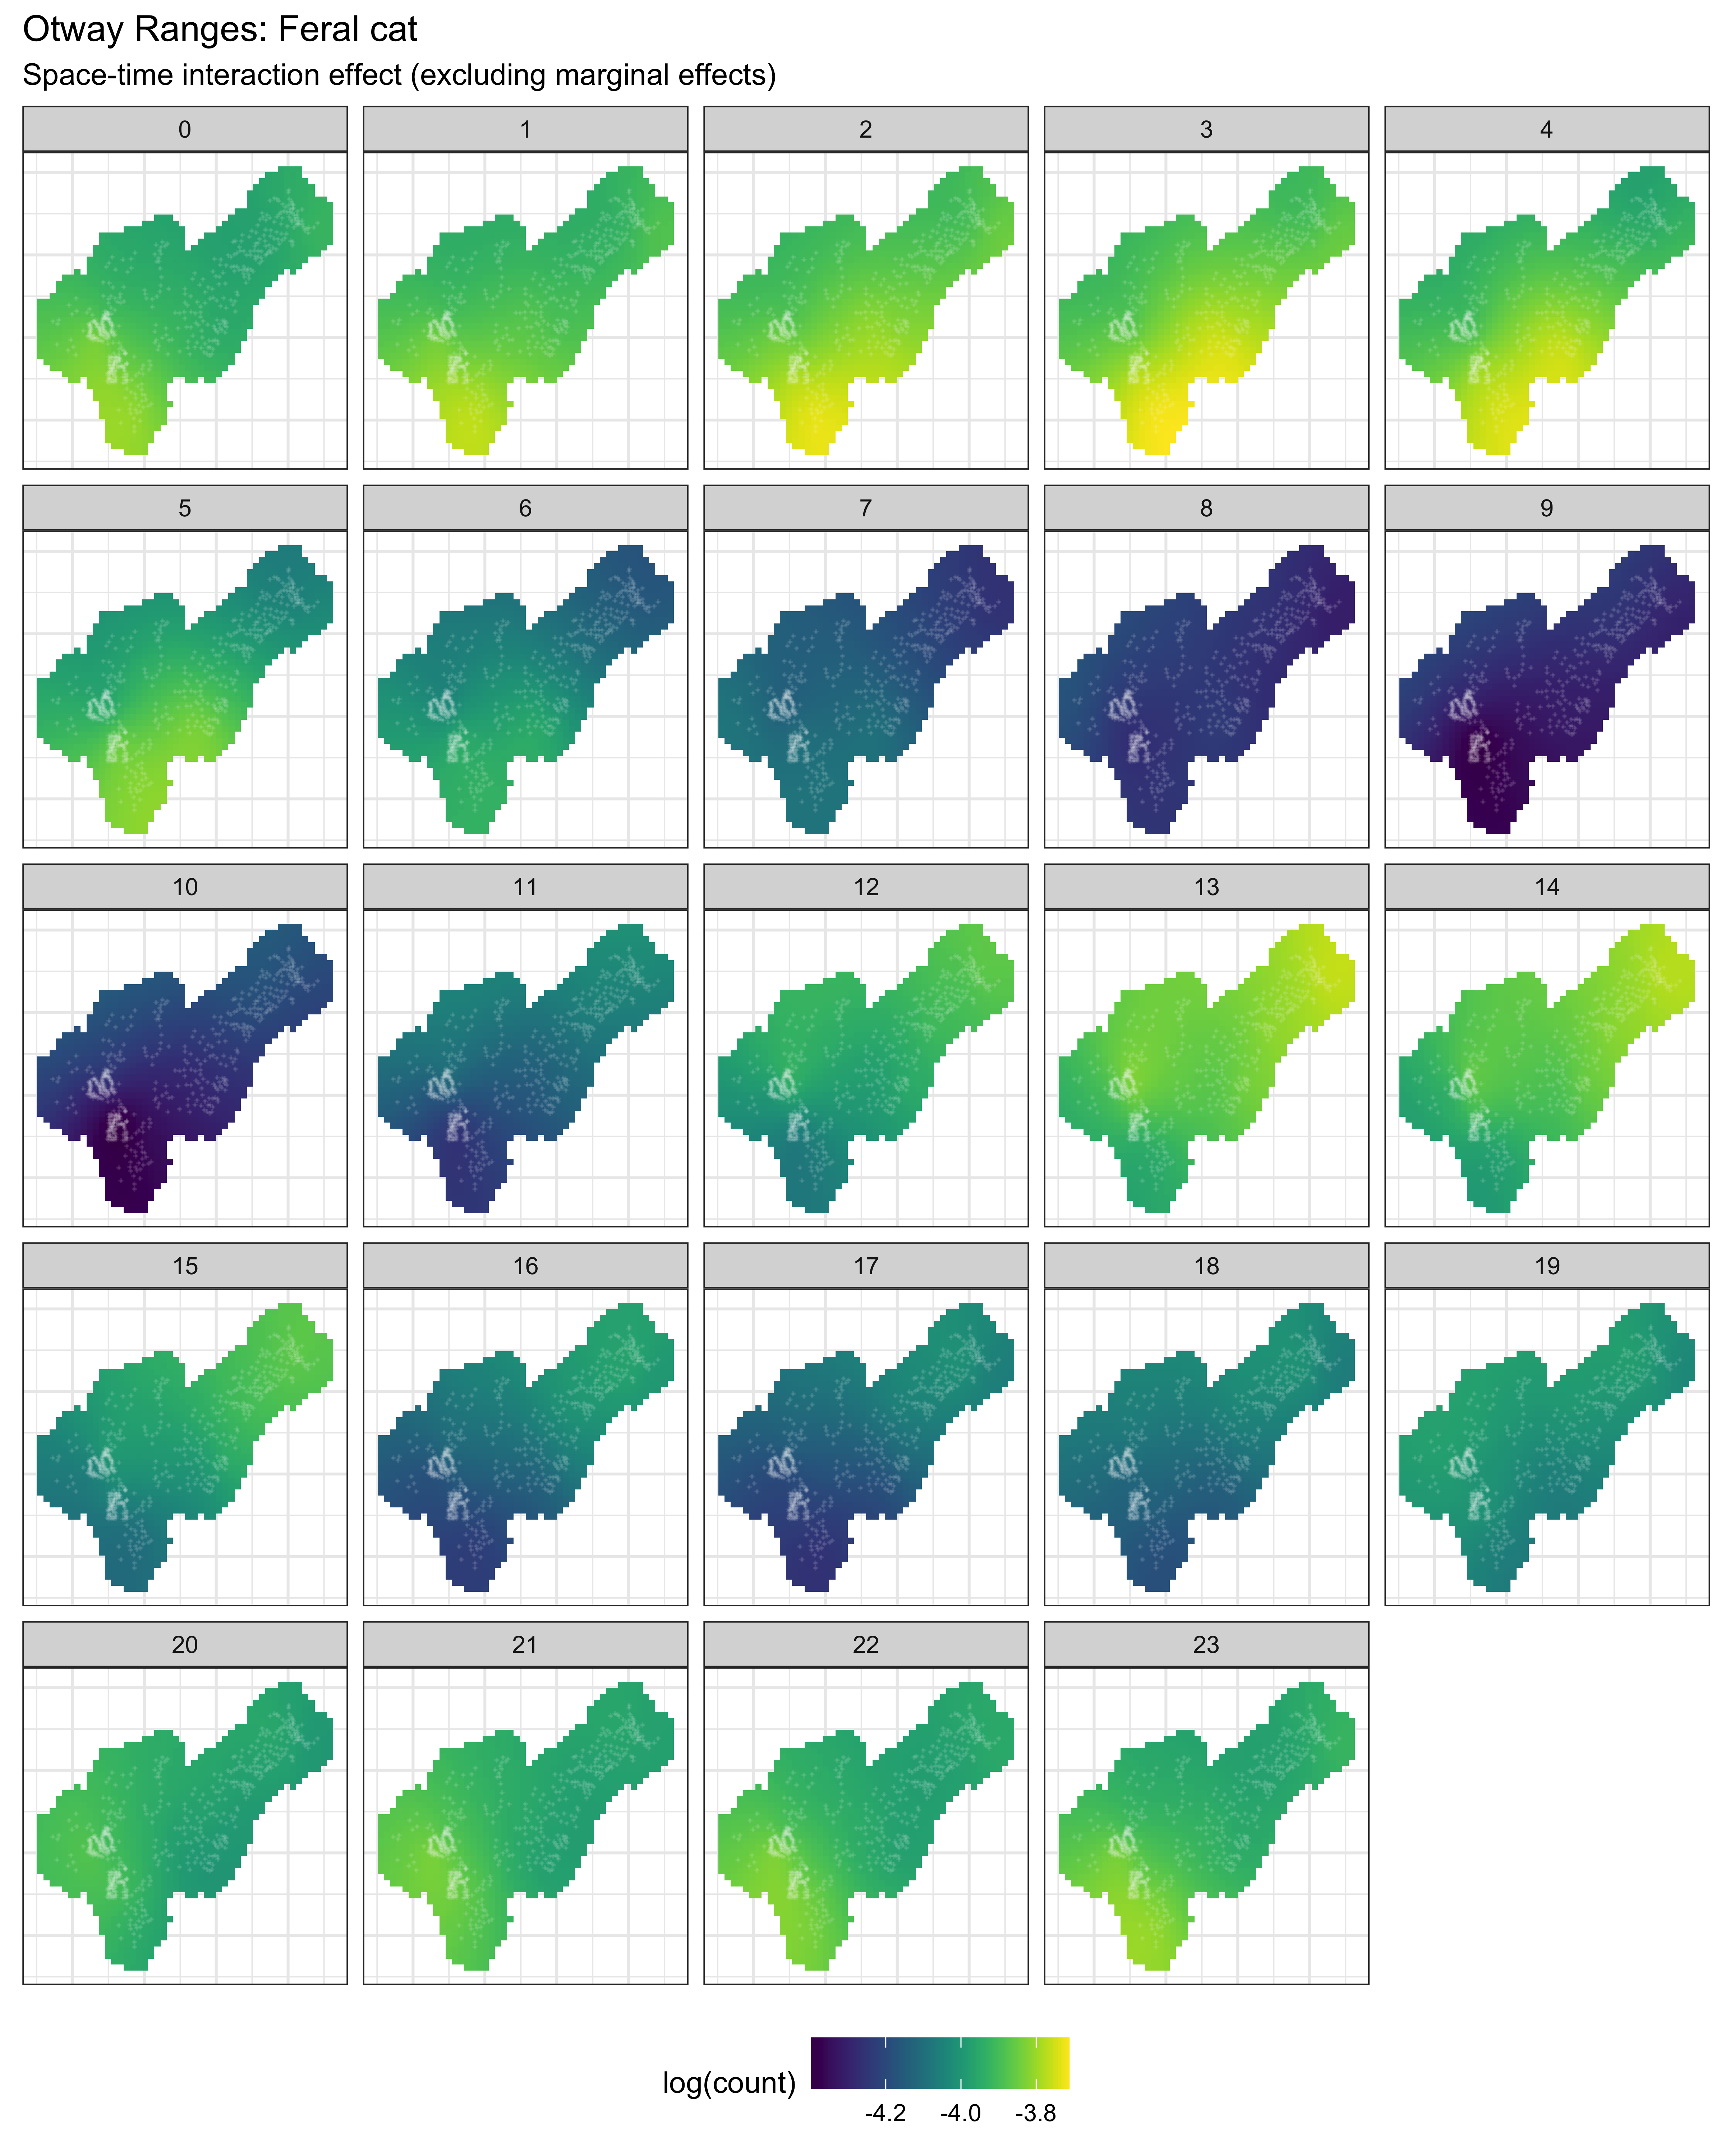
\includegraphics[width=1\linewidth]{figure/spte_diff_avg_o_cat} 

}

\caption{Interaction effect of space-time on feral cat \textit{Felis catus} activity across each hour of the day (0 - 23) in the Otway Ranges, Australia (model 1). White crosses depict unique camera-trap sites. }\label{fig:diel-st-int-o-cat}
\end{figure}
\newpage
\begin{figure}

{\centering 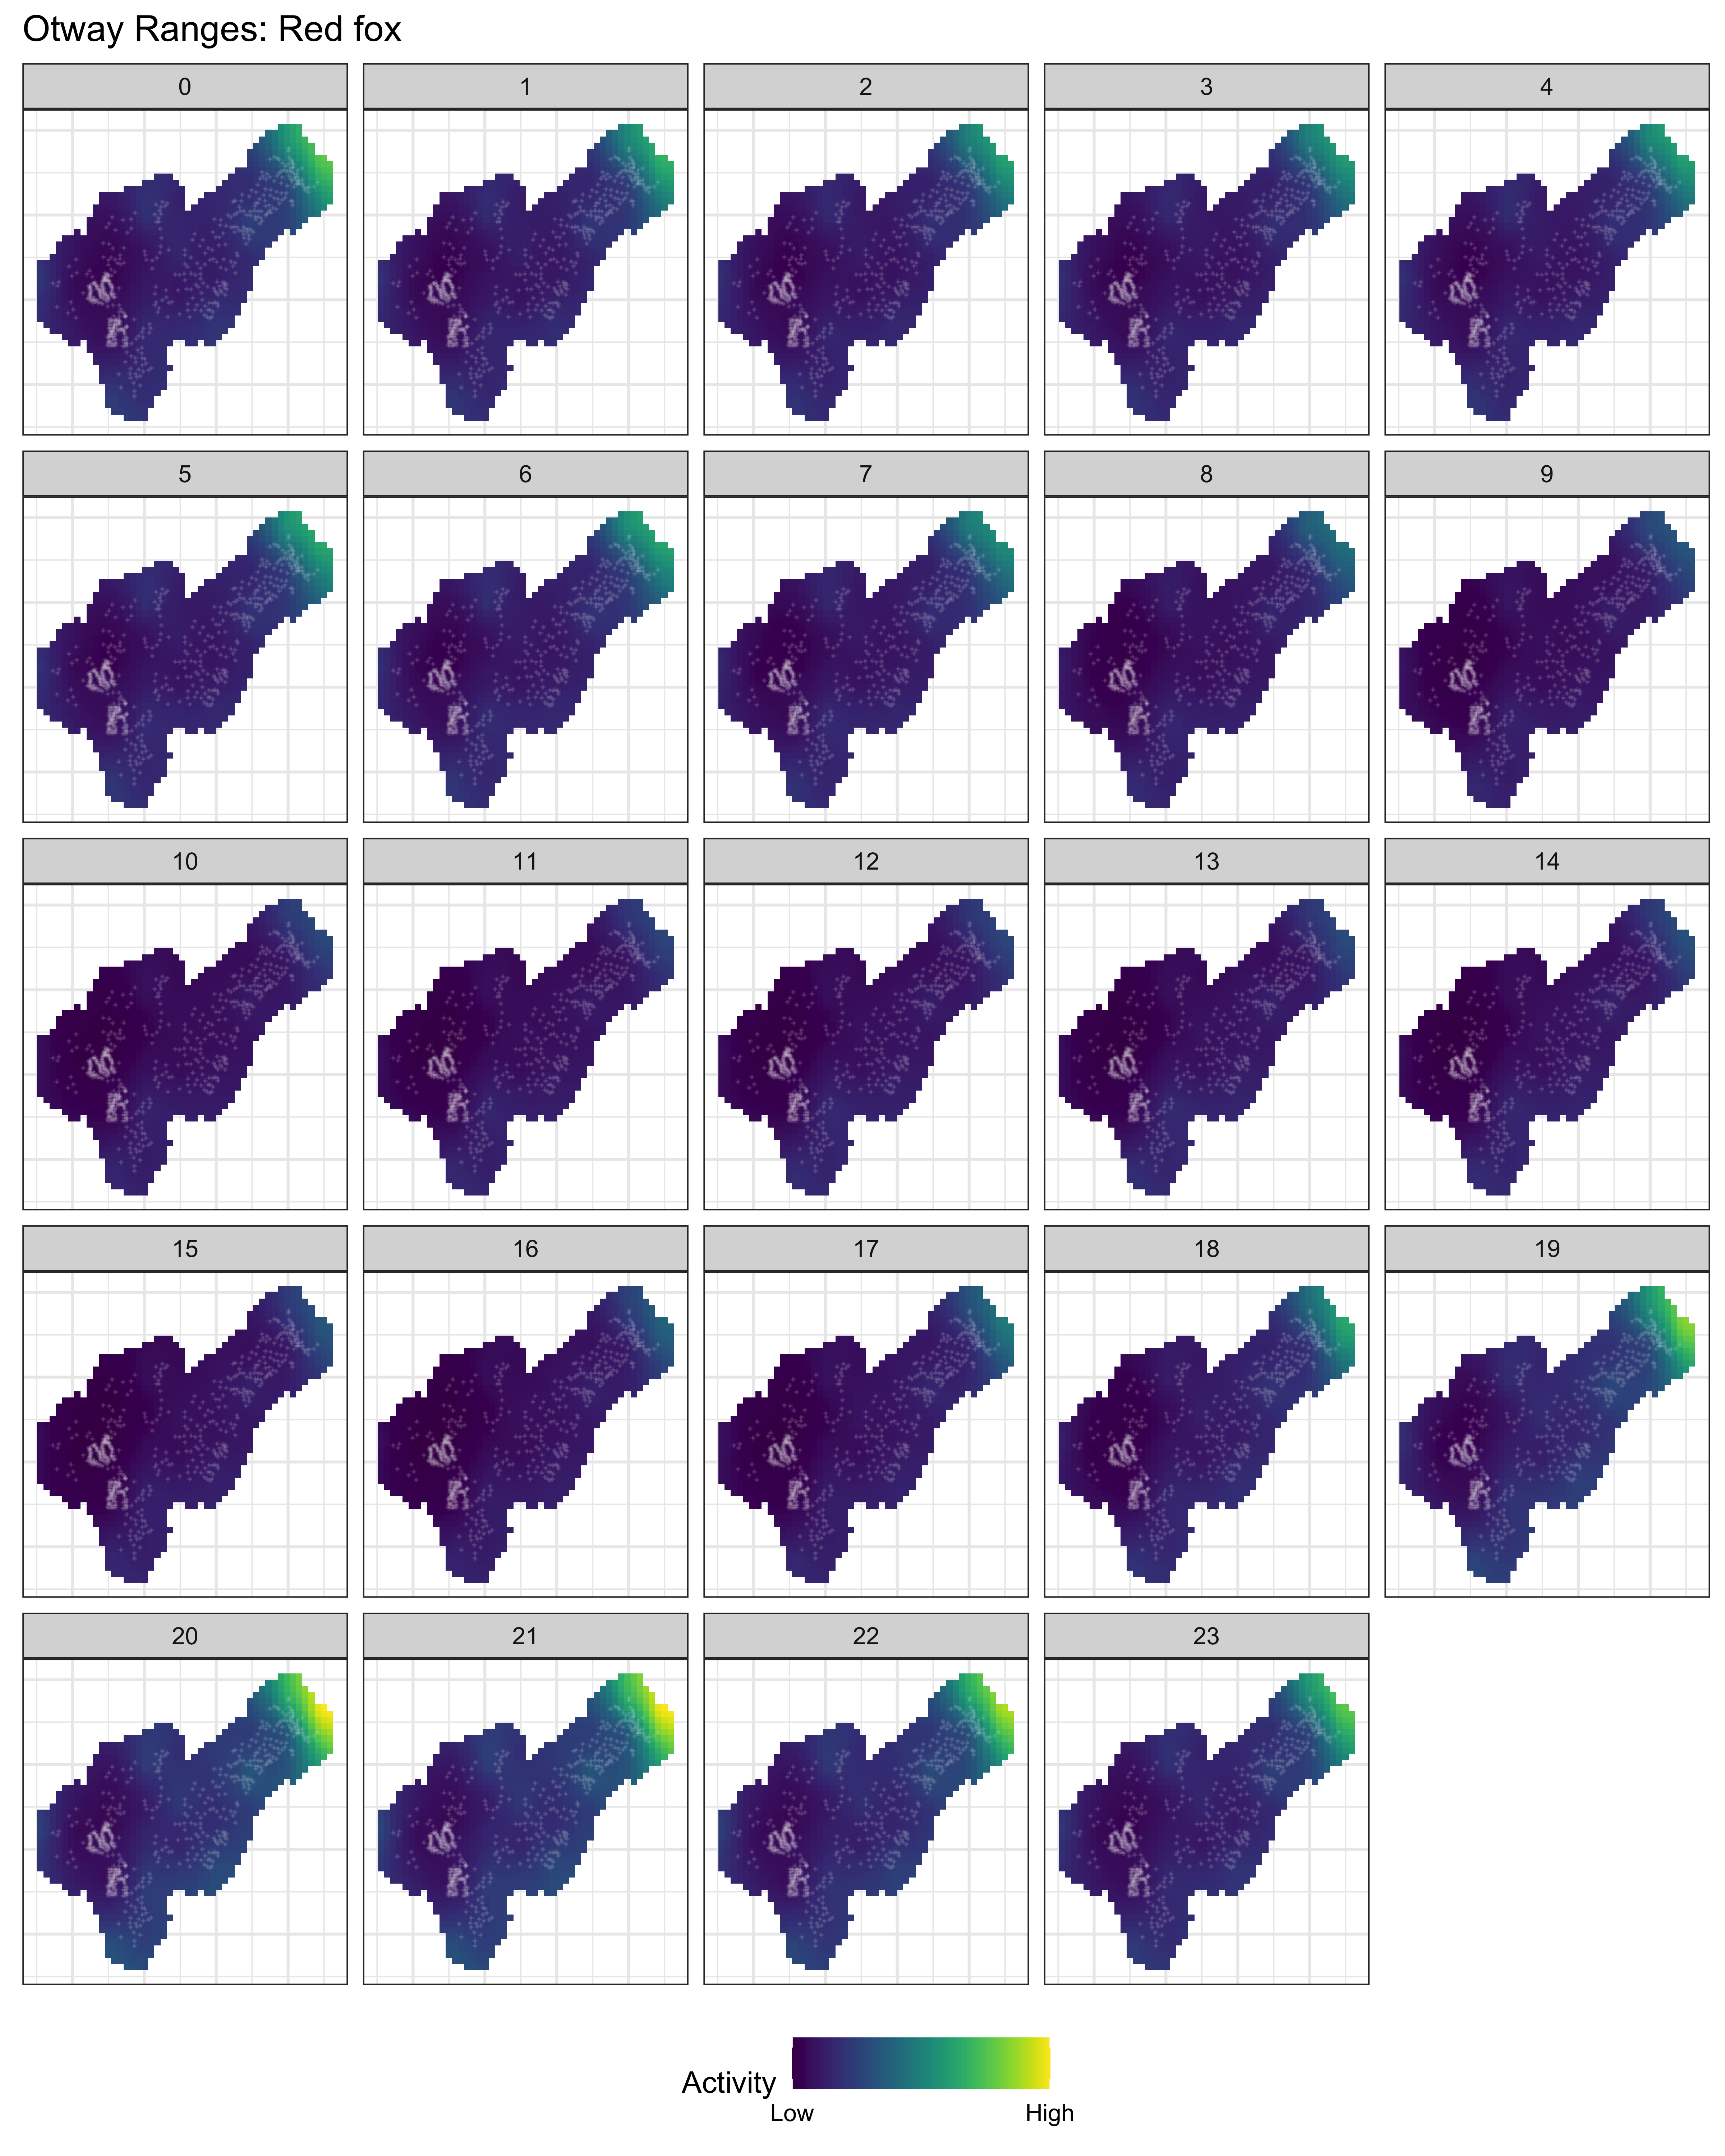
\includegraphics[width=1\linewidth]{figure/spte_facet_o_fox} 

}

\caption{Overall spatial activity of red foxes \textit{Vulpes vulpes} for each hour of the day (0 - 23) in the Glenelg region, Australia (model 1). White crosses depict unique camera-trap sites}\label{fig:diel-space-g-fox}
\end{figure}
\newpage
\begin{figure}

{\centering 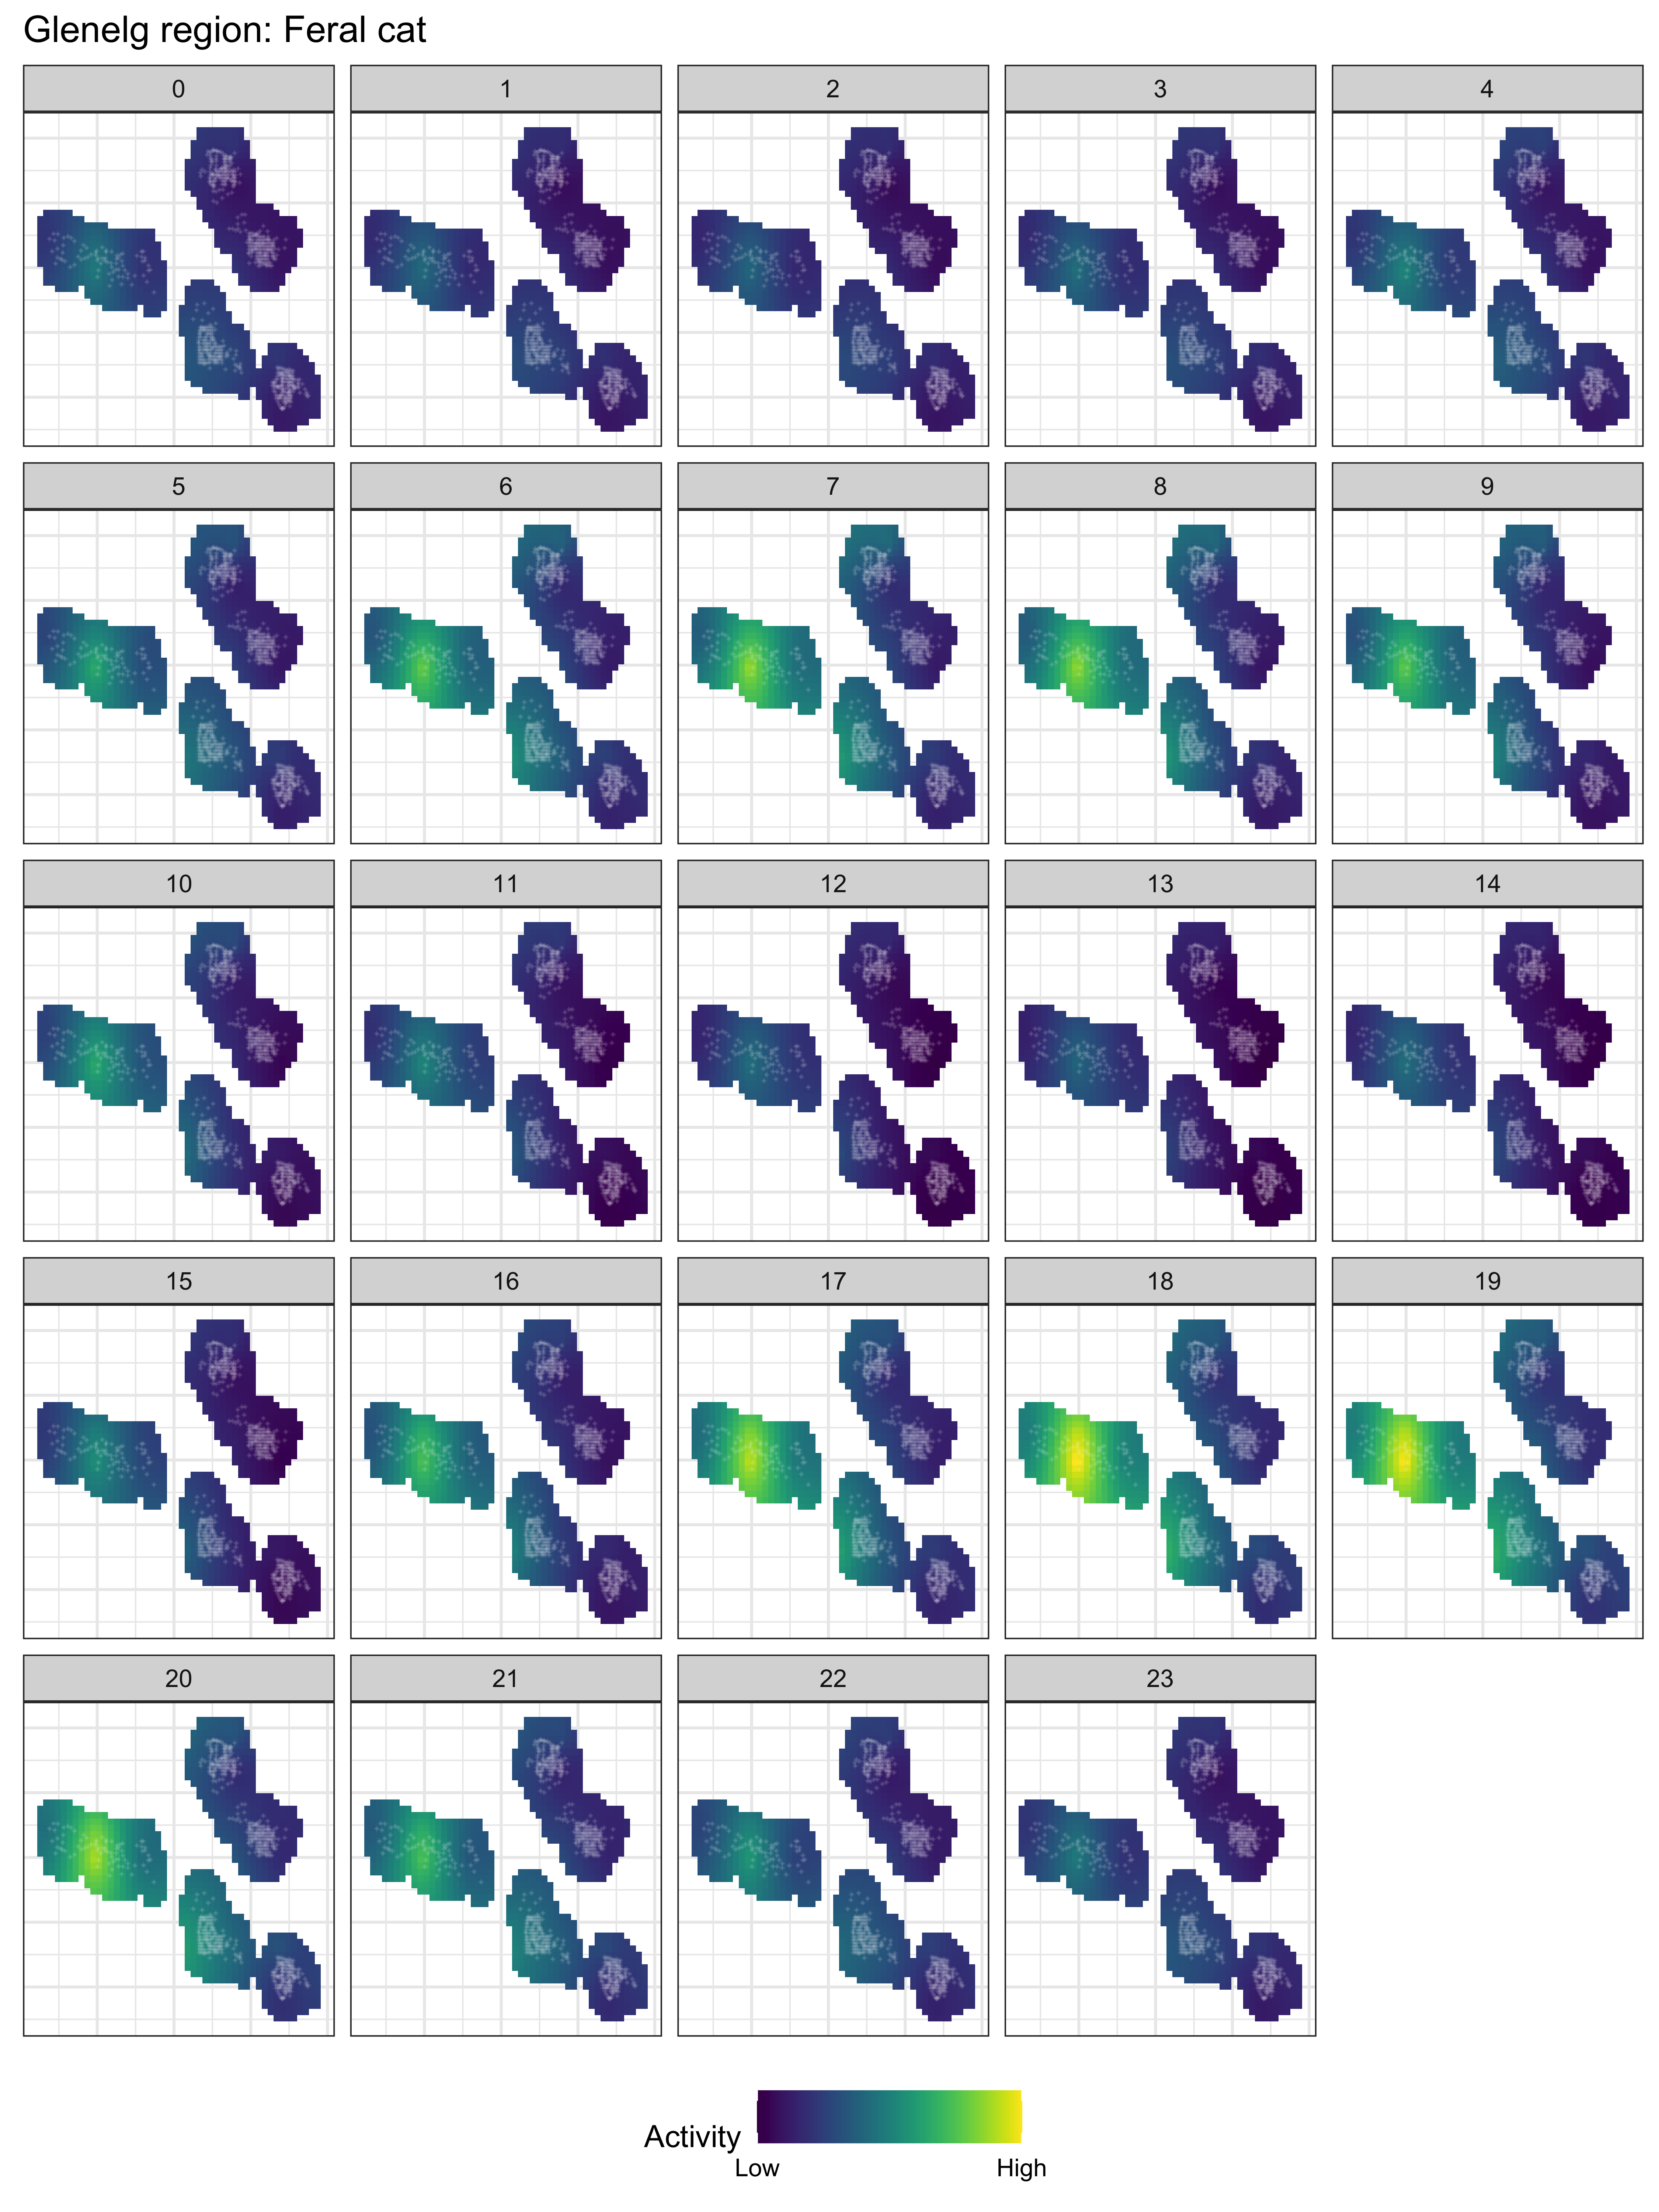
\includegraphics[width=1\linewidth]{figure/spte_facet_g_cat} 

}

\caption{Overall spatial activity of feral cats \textit{Felis catus} for each hour of the day (0 - 23) in the Glenelg region, Australia (model 1). White crosses depict unique camera-trap sites}\label{fig:diel-space-g-cat}
\end{figure}
\newpage
\begin{figure}

{\centering 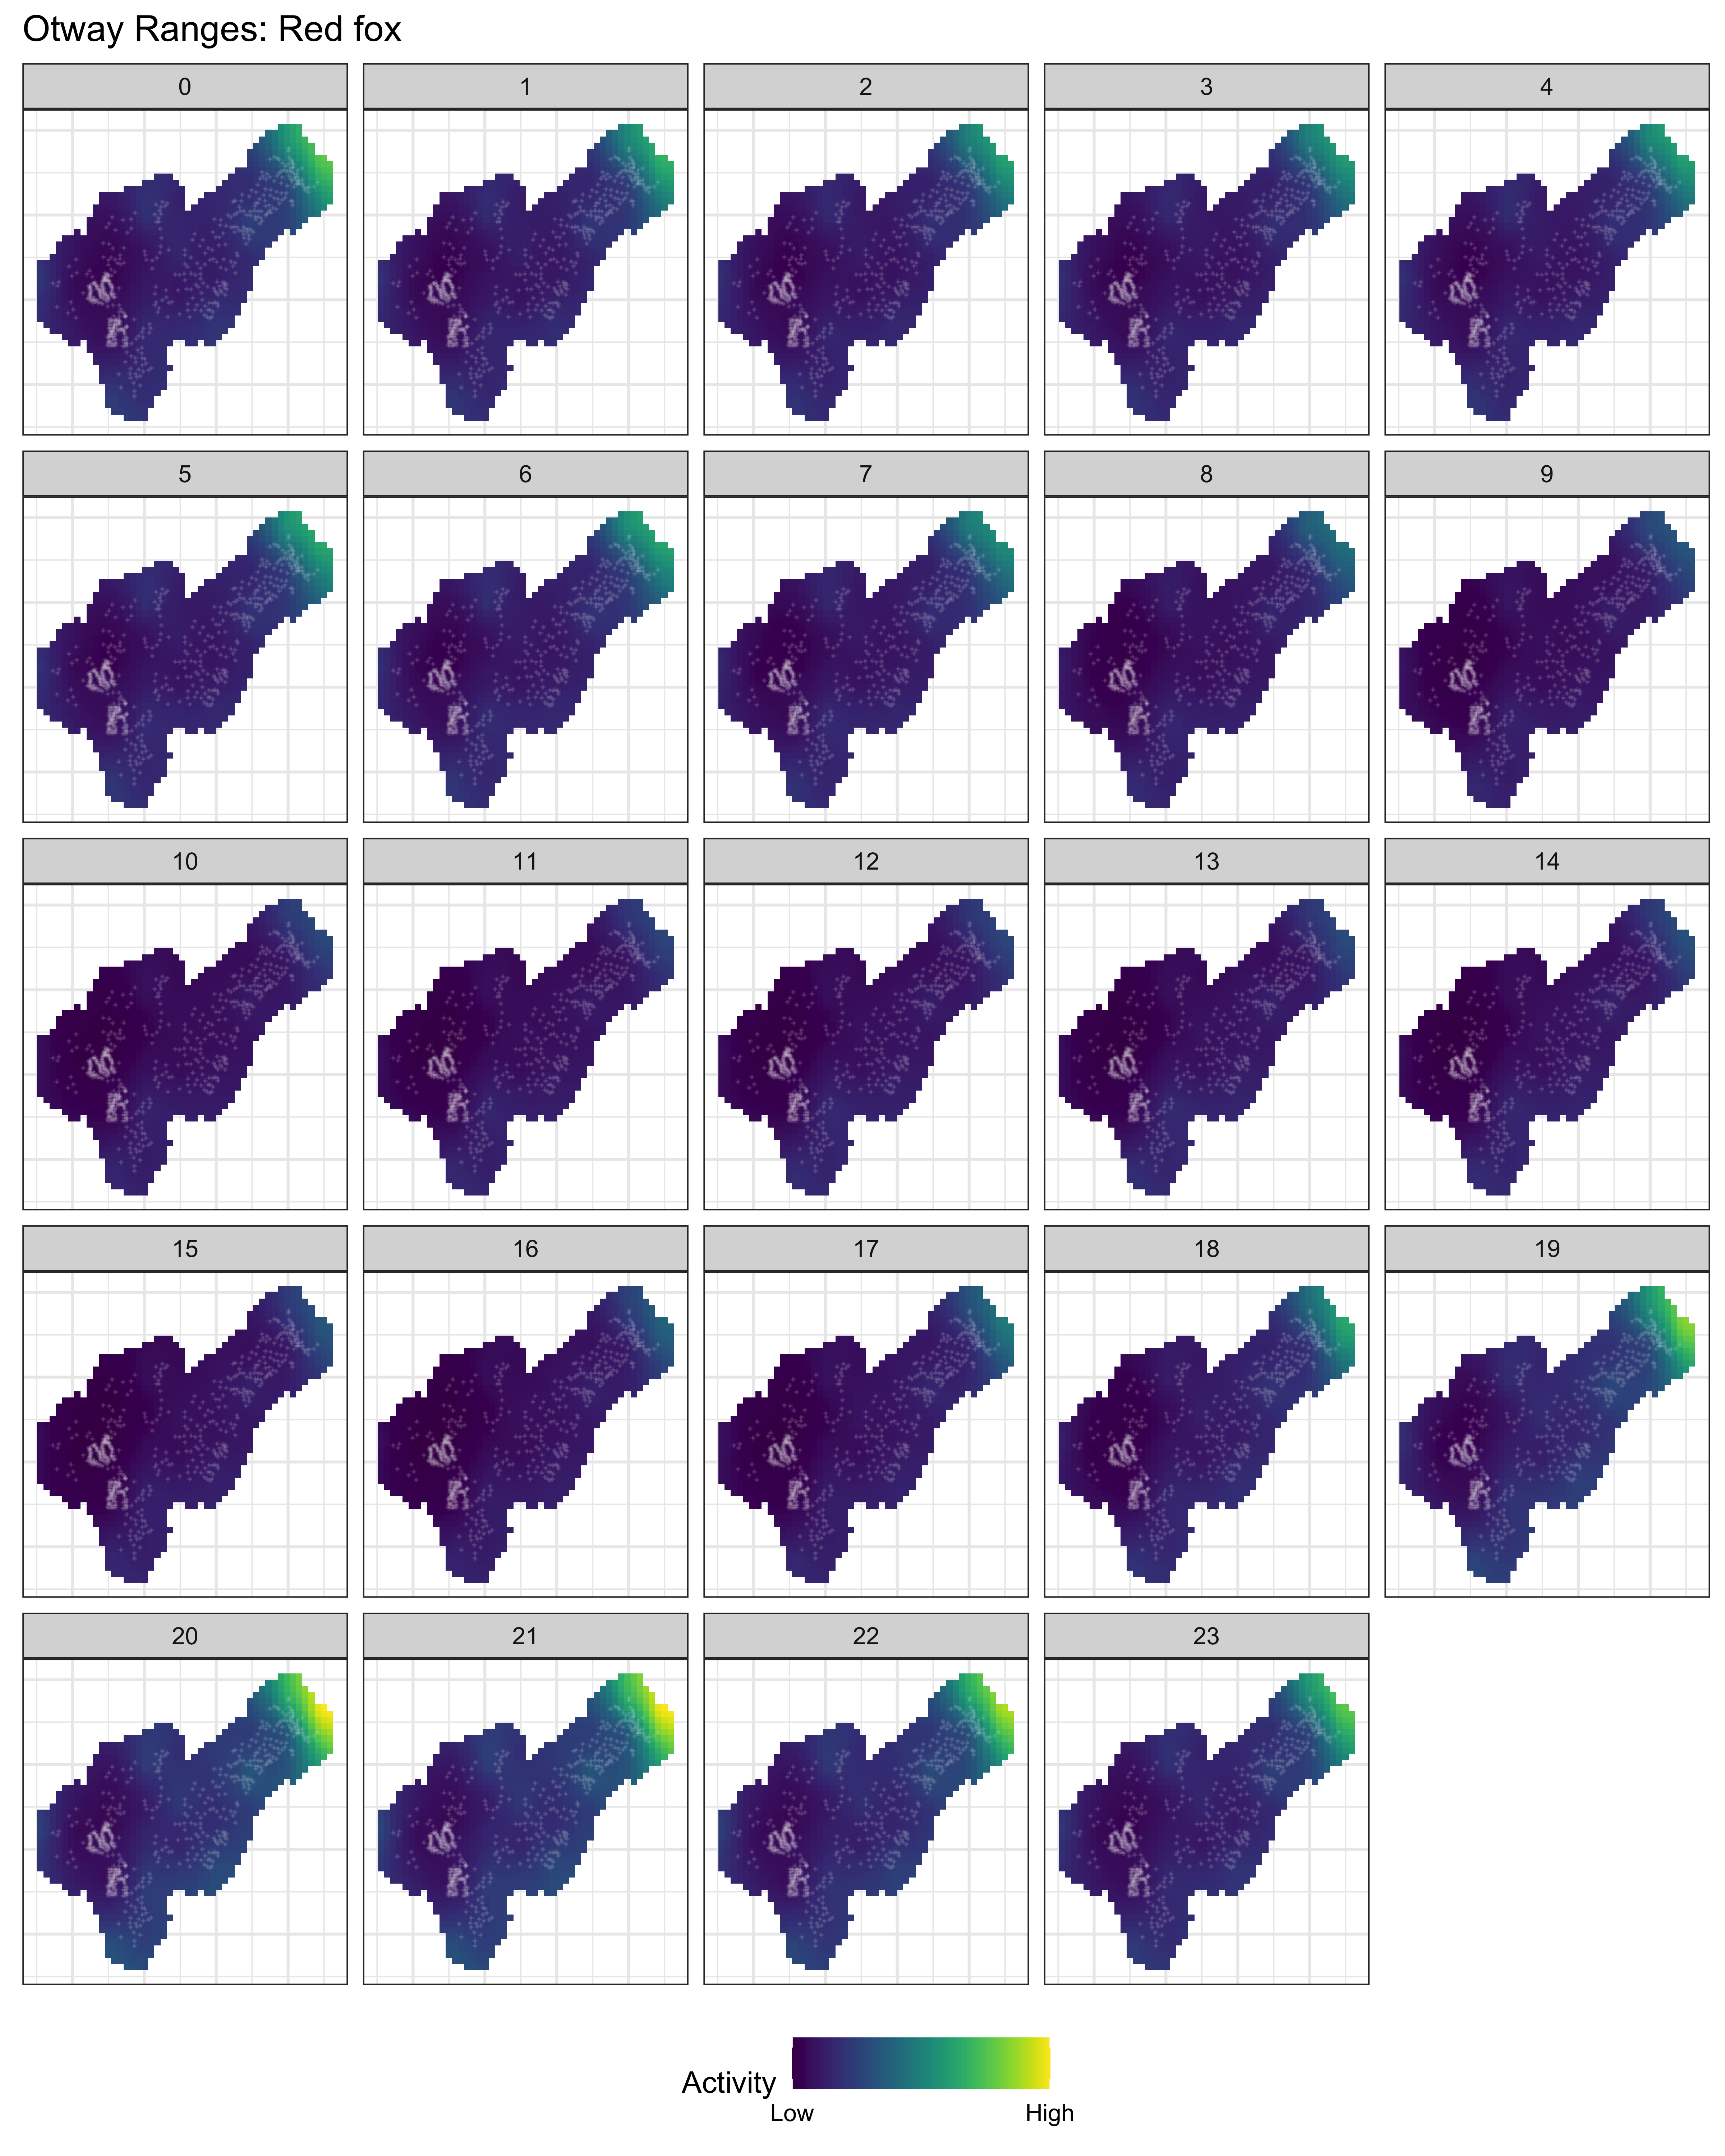
\includegraphics[width=1\linewidth]{figure/spte_facet_o_fox} 

}

\caption{Overall spatial activity of red foxes \textit{Vulpes vulpes} for each hour of the day (0 - 23) in the Otway Ranges, Australia (model 1). White crosses depict unique camera-trap sites}\label{fig:diel-space-o-fox}
\end{figure}
\newpage
\begin{figure}

{\centering 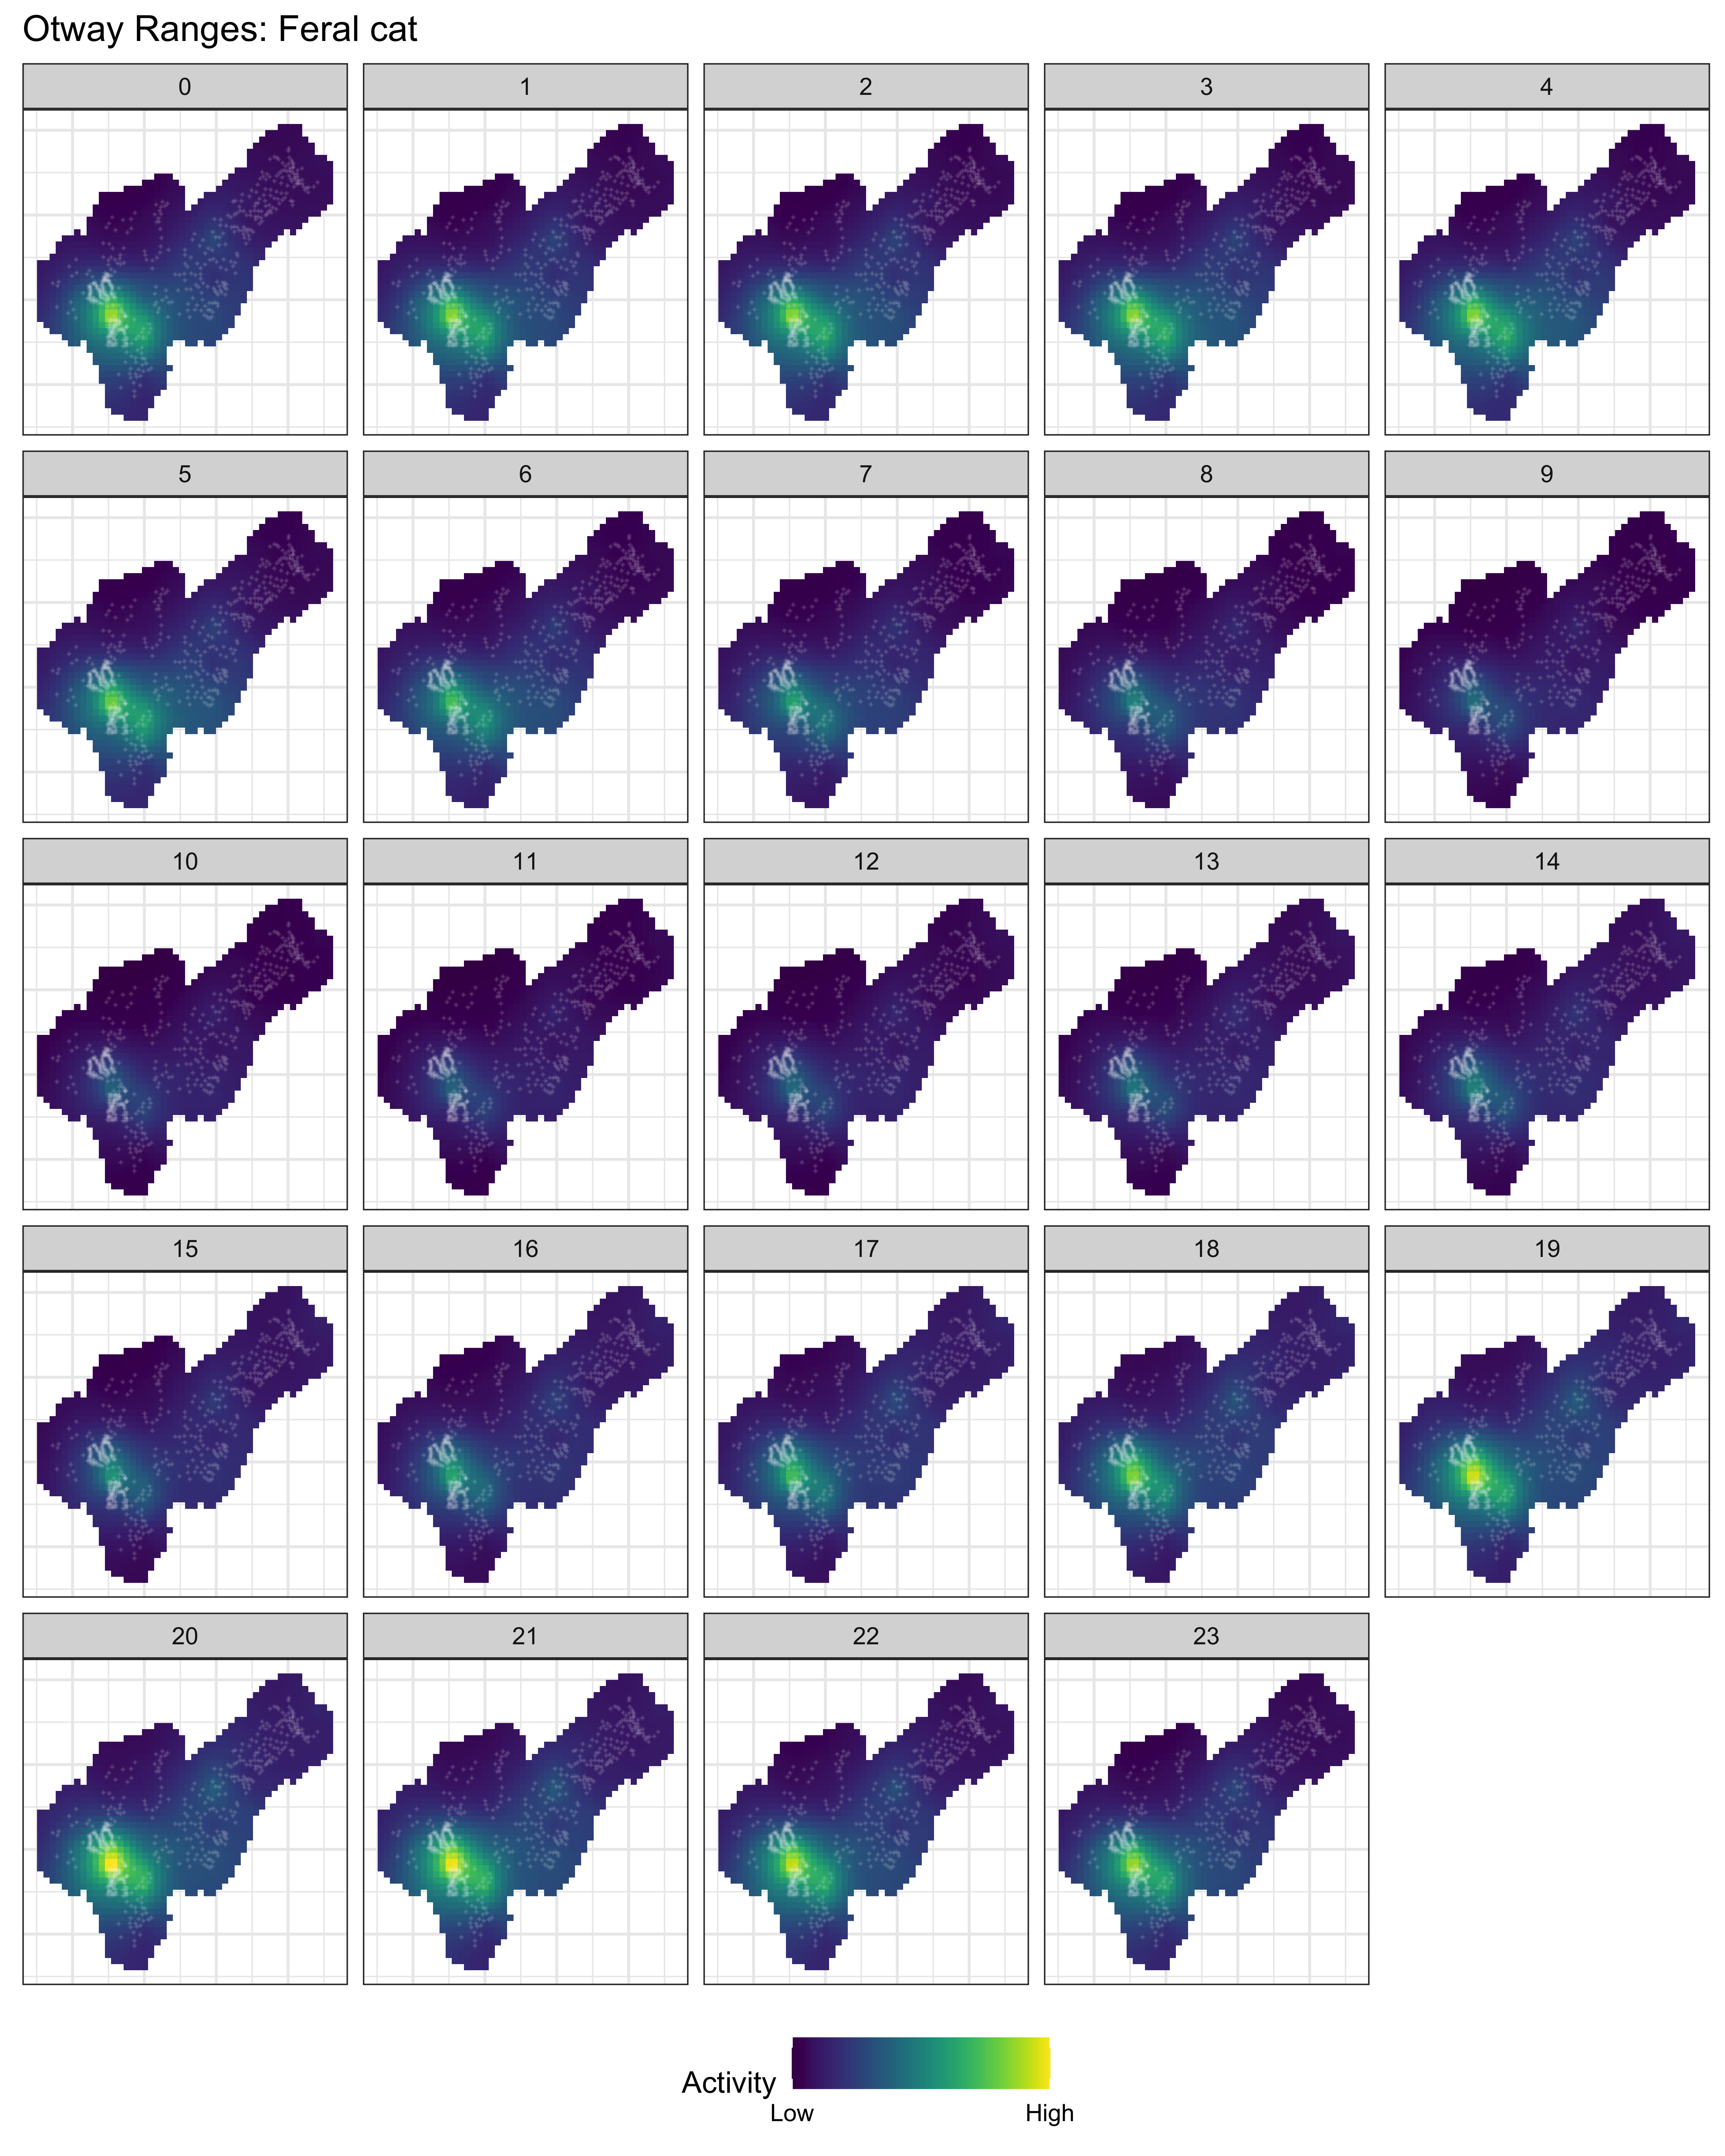
\includegraphics[width=1\linewidth]{figure/spte_facet_o_cat} 

}

\caption{Overall spatial activity of feral cats \textit{Felis catus} for each hour of the day (0 - 23) in the Otway Ranges, Australia (model 1). White crosses depict unique camera-trap sites}\label{fig:diel-space-o-cat}
\end{figure}
\end{mainmatter}
\end{document}
